\documentclass[xcolor=table]{beamer} % "Beamer" is a word used in Germany to mean video projector. 


%%%%%%%%%%%%%%%%%%%%%%%%%%%%%%%%%%%%%%%%%%%%%%%%%%
% N.B. : to compile these slides, you should use
%        lualatex -shell-escape ot_lddmm.tex
%        bibtex ot_lddmm
%        lualatex -shell-escape ot_lddmm.tex
%
% Don't forget to install the 'metropolis' theme from github.
% If the file is a tad too heavy, you can try
% to use the pre-rendered 'pdfpc' for display.
%
% Cheers,
%                    Jean.
%%%%%%%%%%%%%%%%%%%%%%%%%%%%%%%%%%%%%%%%%%%%%%%%%%




\RequirePackage{luatex85}

\usetheme{metropolis} % Search online for beamer themes to find your favorite or use the Berkeley theme as in this file.

\setsansfont{Overlock} % cute !
%\setsansfont{Alegraya Sans}

\usepackage{color} % It may be necessary to set PCTeX or whatever program you are using to output a .pdf instead of a .dvi file in order to see color on your screen.
\usepackage[utf8x]{inputenc}   % LaTeX, comprends les accents !
%\usepackage[T1]{fontenc}      % Police contenant les caractères français
\usepackage[english]{babel}  % Placez ici une liste de langues, la
                              % dernière étant la langue principale
\usepackage{marginnote}
\usepackage{graphicx}
\usepackage{multimedia}

\usepackage{tikz}
\usepackage{pgffor}
\newcommand\mytikzmark[3][]{%
  \tikz[remember picture,baseline=(#2.base)]{\node(#2)[outer sep=0pt,#1]{#3};}%
}
\usepackage{adjustbox}

\usepackage{minted}

\usepackage{float}
\usepackage{amsmath}
\usepackage{amsfonts}
\usepackage{amssymb}
\usepackage{amsthm}
\usepackage{mathtools}
\usepackage{subcaption}
\usepackage{hyperref}
\usepackage[normalem]{ulem}
\usepackage{makecell}
% \usepackage{enumitem}
\usepackage{tikz,float}
\usetikzlibrary{fit,shapes.misc}
\usepackage{centernot}
\usepackage{nccmath}

\newcommand\marktopleft[1]{%
    \tikz[overlay,remember picture] 
        \node (marker-#1-a) at (0,1.0ex) {};%
}
\newcommand\markbottomright[1]{%
    \tikz[overlay,remember picture] 
        \node (marker-#1-b) at (0,0) {};%
    \tikz[overlay,remember picture,thick,dashed,inner sep=3pt]
        \node[draw,rounded rectangle,fit=(marker-#1-a.center) (marker-#1-b.center)] {};%
}
% \usepackage[dvipsnames]{xcolor}

\newcommand\marktopleftone[1]{%
    \tikz[overlay,remember picture] 
        \node (marker-#1-a) at (0,1.5ex) {};%
}

\newcommand\markbottomrightone[1]{%
    \tikz[overlay,remember picture] 
        \node (marker-#1-b) at (0,0) {};%
    \tikz[overlay,remember picture,thick,dashed,inner sep=3pt]
        \node[draw,rounded rectangle,fit=(marker-#1-a.center) (marker-#1-b.center)] {};%
}

\DeclarePairedDelimiterX{\norm}[1]{\lVert}{\rVert}{#1}

% \setbeamercolor{itemize item}{fg=NavyBlue}
\setbeamertemplate{itemize item}[triangle]

\usepackage{todonotes}
\presetkeys{todonotes}{inline}{}

\usepackage{blkarray}% http://ctan.org/pkg/blkarray
\newcommand{\matindex}[1]{ {\scriptstyle #1}}% Matrix index


\usepackage{nicefrac} % 1/2 symbol
\newcommand{\unsdeux}{\nicefrac{1}{2}}

\renewcommand{\epsilon}{\varepsilon}
\newcommand*{\QEDA}{\hfill\ensuremath{\blacksquare}}%

\NewDocumentCommand{\statcirc}{ O{#2} m }{%
    \begin{tikzpicture}
    \fill[#2] (0,0) circle (0.75ex); % Fill circle with base colour (arg#2)
    \fill[#1] (0,0) -- (180:0.75ex) arc (180:0:0.75ex) -- cycle; % Fill a half circle filled with second colour (arg#1), if specified
    \end{tikzpicture}
}


\newcommand{\mine}[1]{\underset{#1~}{\text{\upshape{min}}^\epsilon}~}
\definecolor{oma}{RGB}{0,100,0}
\newcommand{\oma}[1]{\textcolor{oma}{#1}}
\definecolor{omb}{RGB}{0,0,200}
\newcommand{\omb}[1]{\textcolor{omb}{#1}}


\renewcommand{\d}{\text{d}}
\newcommand{\R}{\mathbb{R}}
\newcommand{\Q}{\mathbb{Q}}
\newcommand{\Z}{\mathbb{Z}}
\newcommand{\N}{\mathbb{N}}
%\newcommand{\C}{\mathbb{C}}
\newcommand{\telque}{~|~}
\newcommand{\ilexiste}{\exists~}
\newcommand{\pourtout}{\forall~}
\newcommand{\non}{\neg\,}
\newcommand{\conv}{\star}
\renewcommand{\t}[1]{#1^{\mathsf{T}}}
\renewcommand{\phi}{\varphi}
\newcommand{\fou}[1]{\widehat{#1}}
\newcommand{\zp}[2][p]{%
  \!\IfStrEqCase{#1}{%
    {p}{\left(}%
    {c}{\:\left[}%
    {a}{\left\{}%
    {abs}{\left|}%
    {n}{\left\|}%
    {s}{\left<}%
    {i}{\left[\!\left[}%
  }[\left(]%
    #2%
  \IfStrEqCase{#1}{%
    {p}{\right)}%
    {c}{\right]}%
    {a}{\right\}}%
    {abs}{\right|}%
    {n}{\right\|}%
    {s}{\right>}%
    {i}{\right]\!\right]}%
  }[\right)]%
} 

\theoremstyle{definition}
%\newtheorem{definition}{Définition}
\newtheorem{dfn}{Définition}

\theoremstyle{plain}
\newtheorem{theoreme}{Theorem}
% \newtheorem{lemma}{Lemma}

\theoremstyle{remark}
\newtheorem{rque}{Remarque}



\usepackage{algorithm}
\usepackage[noend]{algpseudocode}
\algtext*{EndWhile}% Remove "end while" text
\algtext*{EndIf}% Remove "end if" text
\usepackage{caption}
\DeclareCaptionFormat{myformat}{#3}
% \captionsetup[algorithm]{format=myformat}


\usepackage{appendixnumberbeamer}

\usepackage{booktabs}
\usepackage[scale=2]{ccicons}

\usepackage{pgfplots}
\usepgfplotslibrary{dateplot}

\usepackage{xspace}
\newcommand{\themename}{\textbf{\textsc{metropolis}}\xspace}

\definecolor{x}{RGB}{8,8,153}
\definecolor{y}{RGB}{153,8,8}
\definecolor{c}{RGB}{0,100,0}
\definecolor{k}{RGB}{0,100,0}
\definecolor{q}{RGB}{60,60,200}
\definecolor{v}{RGB}{60,180,200}
\definecolor{p}{RGB}{30,140,210}
%\definecolor{phi}{RGB}{130,130,130}
\definecolor{phi}{RGB}{100,123,139}


\definecolor{gamma}{RGB}{100,123,139}


\definecolor{dblue}{RGB}{0,0,200}
\definecolor{dred} {RGB}{200,0,0}
\definecolor{dgreen} {RGB}{0,150,0}
\definecolor{b}{RGB}{0,0,255}
\definecolor{a} {RGB}{255,0,0}
\definecolor{grayish}{RGB}{150,150,150}

\definecolor{om}{RGB}{0,0,200}
\newcommand{\om}[1]{\textcolor{om}{#1}}

\newcommand{\xc}[1]{\textcolor{x}{#1}}
\newcommand{\yc}[1]{\textcolor{y}{#1}}

\renewcommand{\a}[1]{\textcolor{dred}{#1}}
\renewcommand{\b}[1]{\textcolor{dblue}{#1}}
\renewcommand{\v}[1]{\textcolor{dgreen}{#1}}
\newcommand{\p}[1]{\textcolor{phi}{#1}}

\title{Integrality Gap Instances and Combinatorial Structure of Gilmore-Gomory LP for Bin Packing}
% \title{Thigh gap instances and Cunnilingal Satisfaction of Gilmore-Girls LP for Ass Spanking}
%\subtitle{Les questions à poser}
\date{Masters Thesis Seminar Talk -- 21st January, 2019}
\author{Yash Patel}
\institute{Rheinische Friedrich-Wilhelms-Universität Bonn\\
Thesis Supervisor: Dr. Heiko R{\"o}glin, Dr. Rolf Klein}

\metroset{subsectionpage=progressbar,
          progressbar=frametitle,
          block=fill}

\begin{document}

\maketitle

\begin{frame}{Bin Packing: Definition}

\onslide<1->{\textbf{\b{Input:}} Items with sizes $s_1, s_2, \ldots, s_n \in (0,1]$ with their multiplicities $b_1, b_2, \ldots, b_n \in \mathbb{Z}_{\geq 0}$.}

\onslide<2->{\textbf{\b{Goal:}} Pack items into minimum number of bins of size 1.}\\~\\
% \vspace{0.1cm}
    % \onslide<1->{\begin{center}
    %         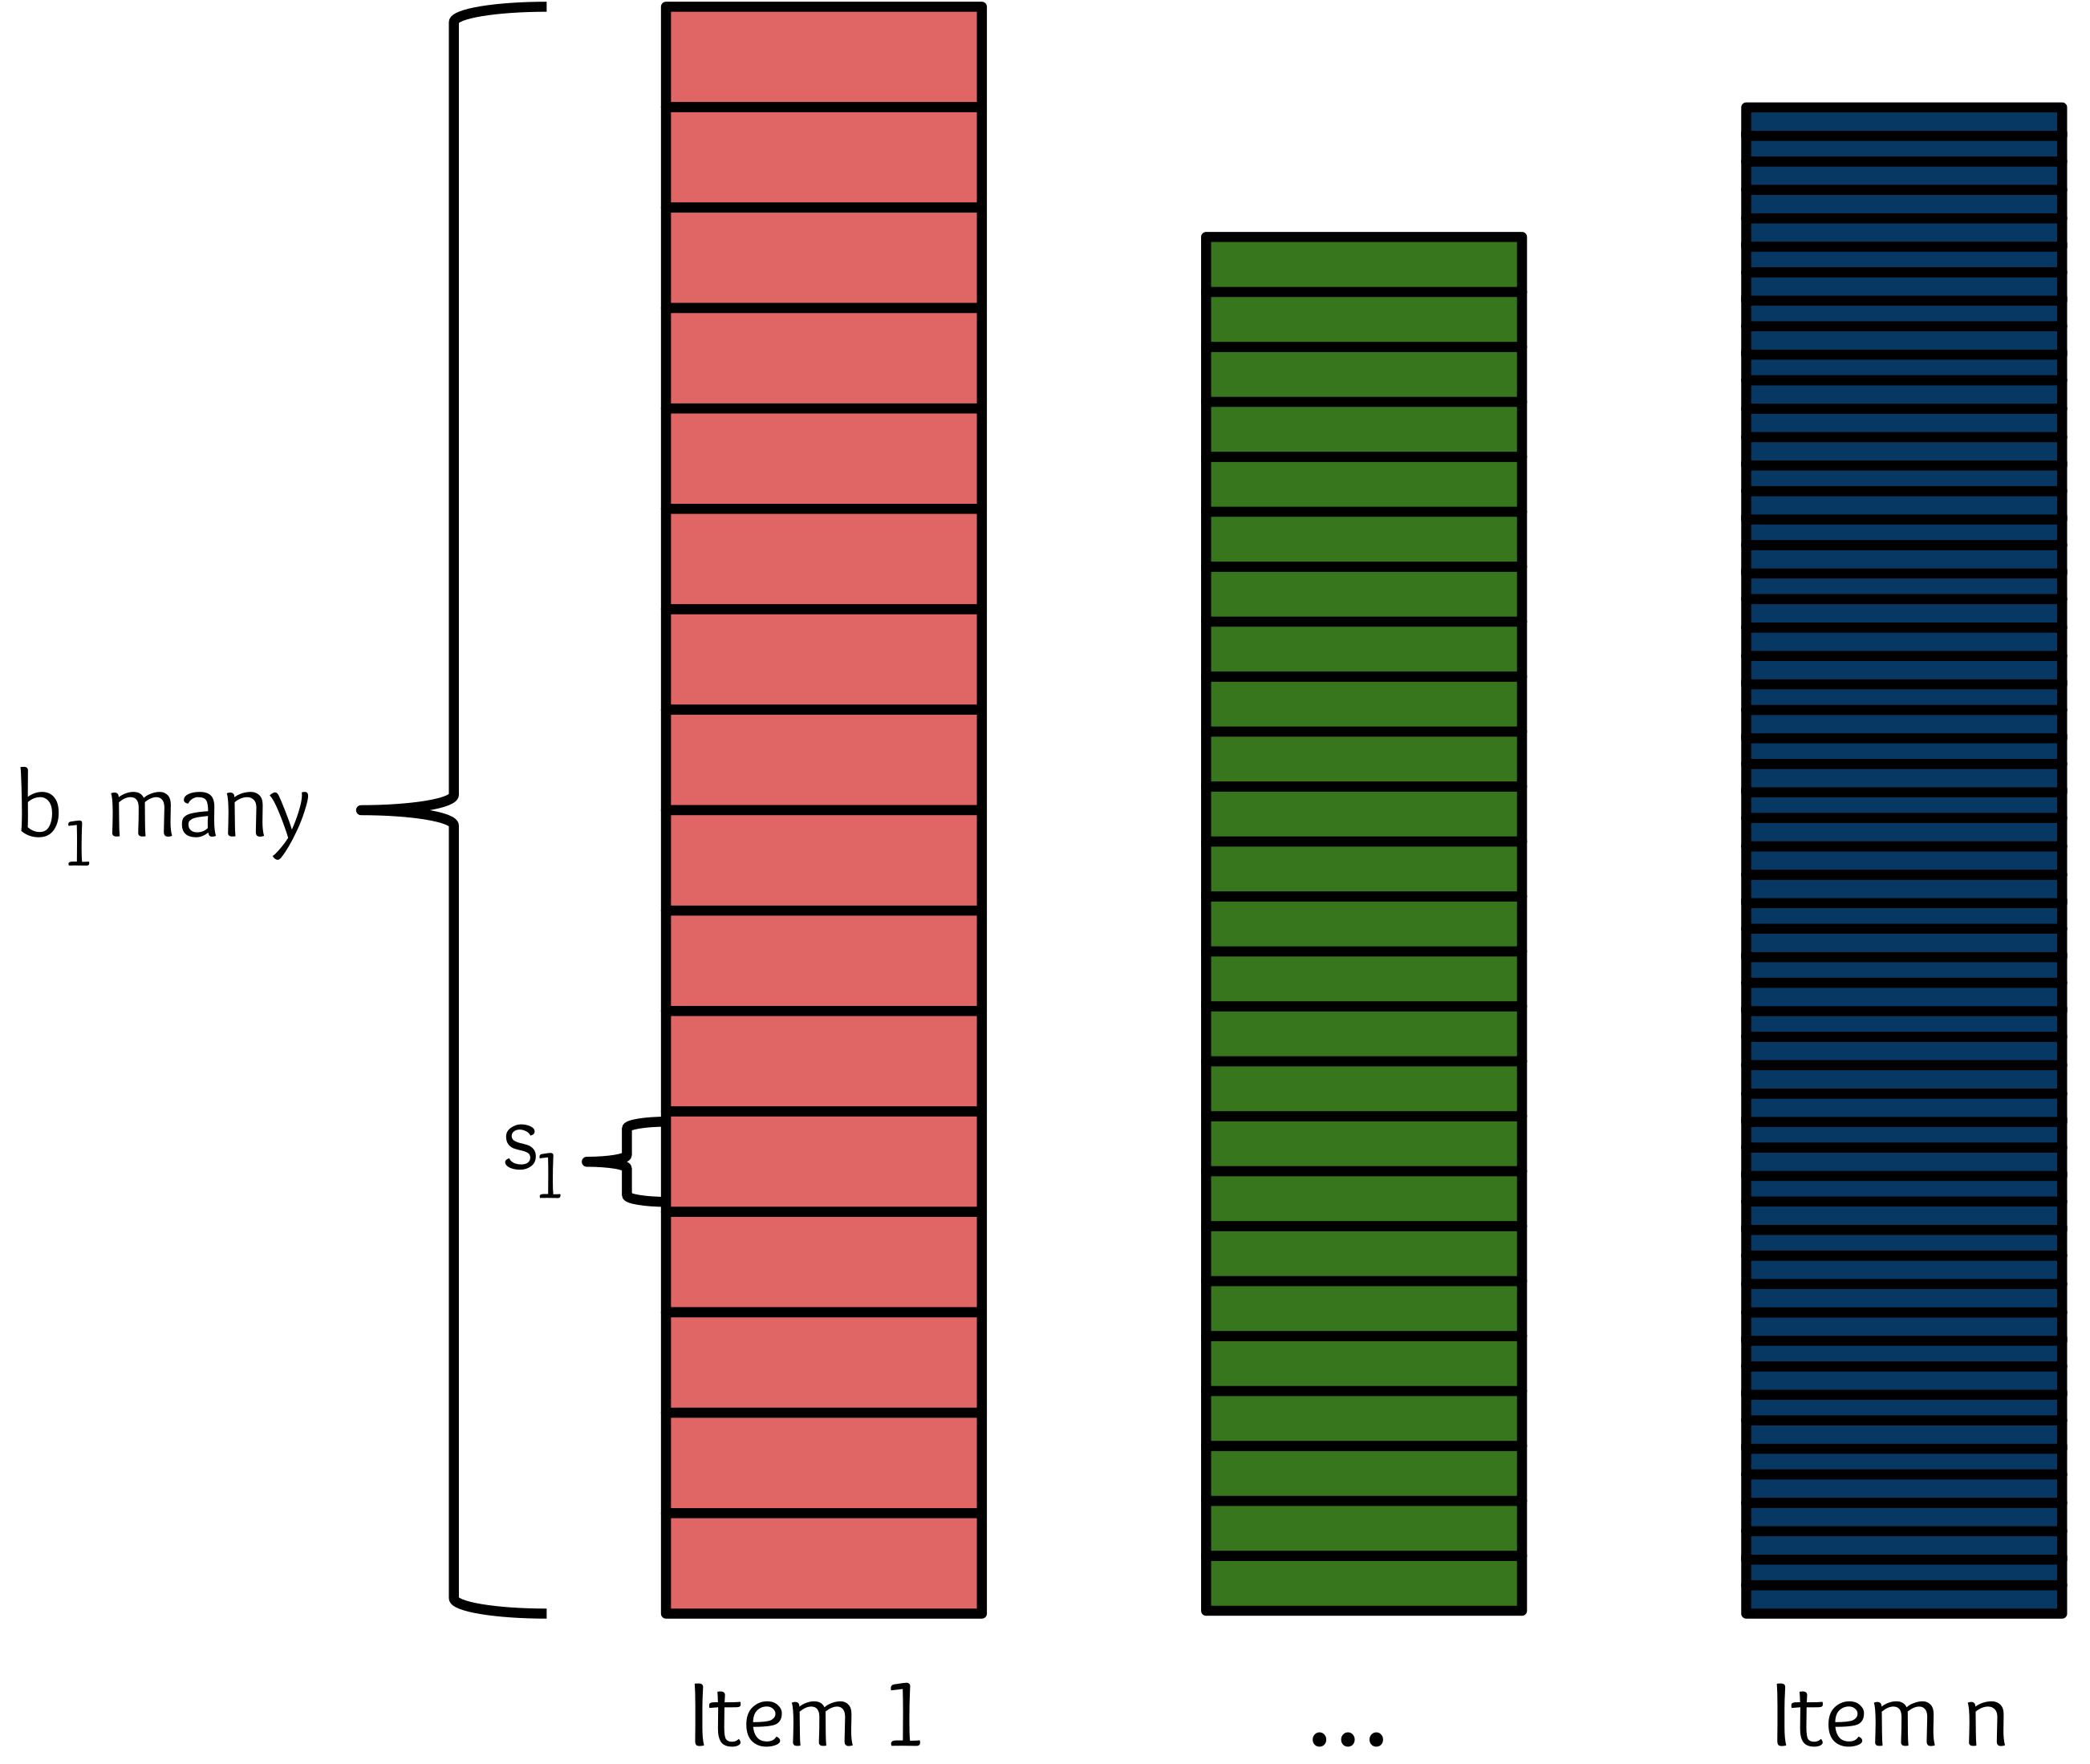
\includegraphics[scale=0.4]{figure/input_bp_tight1.png}
    % \end{center}}
{\begin{tabular}{cl}  
         \begin{tabular}{c}
          \parbox{0.15\linewidth}{%  change the parbox width as appropiate
            \onslide<1->{\textbf{\b{Input:}}}
    }

           \end{tabular}
           & \begin{tabular}{l}
           \centering
            \includegraphics<1,2>[scale=0.4]{figure/input_bp_tight1.png}
            \includegraphics<3>[scale=0.4]{figure/input_bp_pink_empty.png}
            \includegraphics<4>[scale=0.4]{figure/input_bp_pink_green_empty.png}
            \includegraphics<5>[scale=0.4]{figure/input_bp_pink_green_blue_empty.png}
         \end{tabular}  \\
\end{tabular}}
    
    % \begin{center}
    %         \includegraphics<2>[scale=0.4]{figure/empty_bin.png}
    % \end{center}
    
\begin{tabular}{cl}  
         \begin{tabular}{c}
          \parbox{0.15\linewidth}{%  change the parbox width as appropiate
            \onslide<2->{\textbf{\b{Solution:}}}
    }

           \end{tabular}
           & \begin{tabular}{l}
           \centering
            \includegraphics<2>[scale=0.4]{figure/empty_bin.png}
            \includegraphics<3>[scale=0.4]{figure/bin_pink_filled.png}
            \includegraphics<4>[scale=0.4]{figure/bin_pink_green_filled.png}
            \includegraphics<5>[scale=0.4]{figure/bin_pink_green__bluefilled.png}
         \end{tabular}  \\
\end{tabular}




% 	\begin{center}
% 		Source $\a{A}$, target $\b{B}$, \onslide<2->{mapping $\p{\phi}$}

% 		\onslide<5>{
% 		$\a{A}~ \underset{\text{Model}\vphantom{\textbf{Loss}}}{\xrightarrow{~~~~\p{\phi}~~~~}}~\p{\phi(\a{A})}~=~ \a{A'} \underset{\textbf{Loss}}{~\rightleftarrows~} \b{B}$
% 		}
% 		\vspace*{-.2cm}

% 		\only<1>{\includegraphics[height=.75\textheight]{images/registration/frame_0.png}}%
% 		\only<2>{\includegraphics[height=.75\textheight]{images/registration/frame_1.png}}%
% 		\only<3>{\includegraphics[height=.75\textheight]{images/registration/frame_2.png}}%
% 		\only<4>{\includegraphics[height=.75\textheight]{images/registration/frame_3.png}}%
% 		\only<5>{\includegraphics[height=.75\textheight]{images/registration/frame_4.png}}%
% 	\end{center}
\end{frame}

\begin{frame}{Bin Packing: Polynomial Time Algorithms}
\textbf{\b{For general $n$:}}

\begin{itemize}
    
    \item  First Fit Decreasing~\cite{johnson1974worst}: $APX \leq \frac{11}{9}\mathsf{OPT} + 4$
    \pause
    \item  Asymptotic PTAS~\cite{de1981bin}: \\
    $APX \leq (1+\epsilon)\mathsf{OPT} + O(\frac{1}{{\epsilon}^2})$
    \pause
    \item  Asymptotic FPTAS:
    \\
    $APX \leq \mathsf{OPT} + O({\log}^2 n)$~\cite{karmarkar1982efficient} \\
    $APX \leq \mathsf{OPT} + O(\log \cdot \log \log n)$~\cite{rothvoss2013approximating}
    \\
    $APX \leq \mathsf{OPT} + O(\log n)$~\cite{hoberg2017logarithmic}
    % \\
    % (Running time $poly(\sum_{i=1}^n b_i)$, hence pseudo-polynomial)
    \pause
    \item  Strongly $\mathsf{NP}$-hard even if $s_i \in (\frac{1}{4}, \frac{1}{2})$ \a{(3-Partition Case)}
    
\end{itemize}

\end{frame}


\begin{frame}{The Gilmore-Gomory LP Relaxation}
    
    \begin{itemize}
        
        \onslide<1->{\item  Recall that $b_i = \#$ of items of size $s_i$.}
        
        \onslide<1->{\item  \textbf{\b{Feasible Patterns:}}
           
            \begin{center}
                $\mathcal{P} = \{p \in \mathbb{Z}^n_{\geq 0} \mid \sum_{i=1}^{n} s_i \ p_i \leq 1\}$
            \end{center}
            
                \only<1>{\begin{center}
                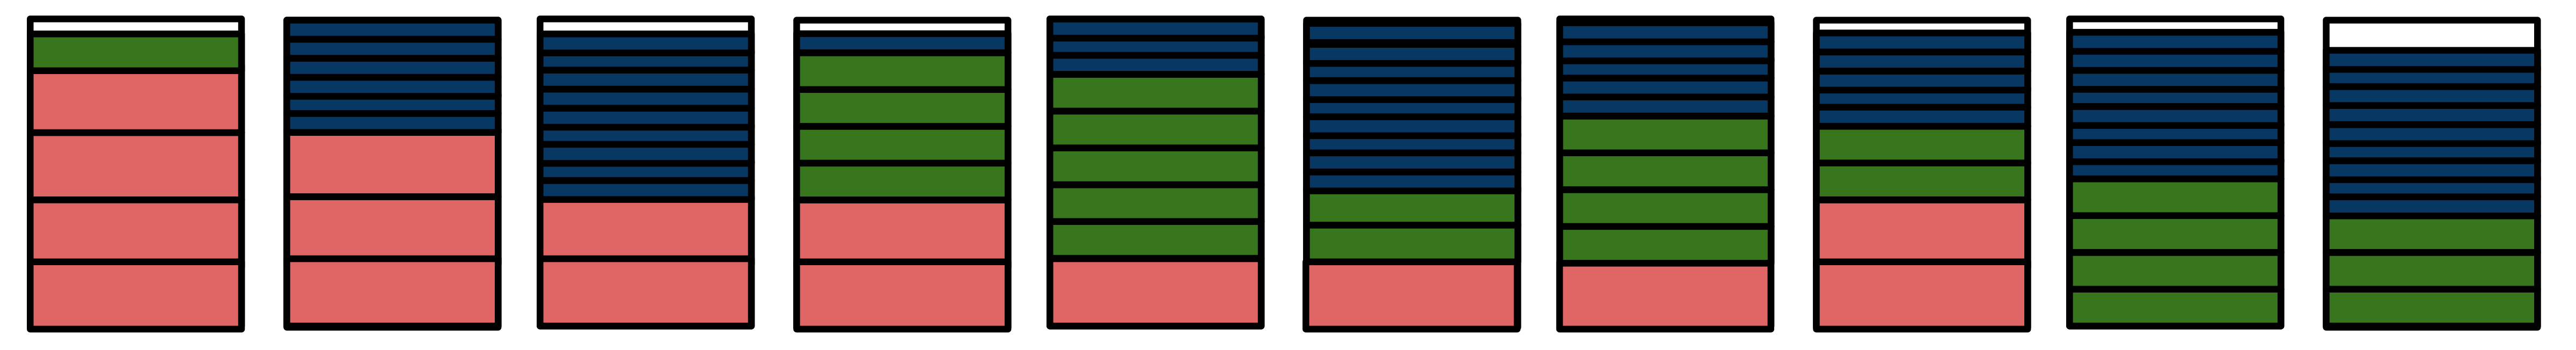
\includegraphics[scale=0.4]{figure/bins-pattern-explain.png}
                \end{center}}
            }
        
        \onslide<2->{\item  \textbf{\b{Gilmore-Gomory LP Relaxation:}}}
                
                \only<2>{\begin{equation*}
                    \begin{aligned}
                        & {\text{min}}
                        & & \sum_{p \in \mathcal{P}} \ x_p &&&& \a{\leftarrow \text{pattern multiplicity}} \\
                        & \text{s.t.} & & \sum_{p \in \mathcal{P}} \ x_p \ p_i = b_i &&&& \forall \ i \in [n] \\
                        & & & x_p \in \mathbb{R}_{\geq 0} &&&& \forall \ p \in \mathcal{P} 
                    \end{aligned}
                \end{equation*}}
                \only<3>{\begin{equation*}
                    \begin{aligned}
                        & {\text{min}}
                        & & \mathbf{1}^{\text{T}} \ x \\
                        & \text{s.t.} & & \mathsf{A} \ x = b \\
                        & & & x_p \in \mathbb{R}_{\geq 0} &&&& \forall \ p \in \mathcal{P} 
                    \end{aligned}
                \end{equation*}}
    
    \end{itemize}
    
\end{frame}


% \begin{frame}{The Gilmore-Gomory LP Relaxation}
    
%     \begin{itemize}
        
%         \item  Recall that $b_i = \#$ of items of size $s_i$
        
%         \item  \textbf{\b{Feasible Patterns:}}
           
%             \begin{center}
%                 $\mathcal{P} = \{p \in \mathbb{Z}^n_{\geq 0} \mid \sum_{i=1}^{n} s_i \ p_i \leq 1\}$
%             \end{center}
        
%         \item  \textbf{\b{Gilmore-Gomory LP Relaxation:}}
                
%                 \begin{equation*}\label{eqn:GGIP}
%                     \begin{aligned}
%                         & {\text{min}}
%                         & & \mathbf{1}^{\text{T}} \ x \\
%                         & \text{s.t.} & & A \ x = b \\
%                         & & & x_p \in \mathbb{R}_{\geq 0} &&&& \forall \ p \in \mathcal{P} 
%                     \end{aligned}
%                 \end{equation*}
    
%     \end{itemize}
    
% \end{frame}


% \begin{frame}{The Gilmore-Gomory LP Relaxation: Example}
    
% \end{frame}

\begin{frame}{The Gilmore-Gomory LP Relaxation: Integrality Gap}
    % \begin{itemize}
        
    %     {\item  \textbf{\b{Gilmore-Gomory LP Relaxation:}}
    %         \begin{equation*}
    %             \begin{aligned}
    %                  \bigg\{{\text{min}}
    %                  \sum_{p \in \mathcal{P}} \ x_p 
    %                  \mid \sum_{p \in \mathcal{P}} \ x_p \ p_i = b_i, \forall \ i \in [n];
    %                 \ x_p \in \mathbb{R}_{\geq 0}, \forall \ p \in \mathcal{P}\bigg\} 
    %             \end{aligned}
    %         \end{equation*}}
                
    % \end{itemize}
    
    {\begin{alertblock}{Modified Integer Round Up Conjecture (MIRUP)}
        $\mathsf{OPT} - \lceil \mathsf{OPT_f} \rceil \leq 1$
    \end{alertblock}}
    
    \begin{itemize}
        \item  {\color{green}True}, if $\#$ of different item types $n \leq  6$\only<1>{\footnote{~\cite{sebo2009proof} claimed to prove for $n \leq 7$, but no manuscript!}}
        
        \item  Best known upper bound: $\mathsf{OPT} - \mathsf{OPT_f} \leq O(\log n)$
        
        \onslide<2->{\item  \textbf{\b{Additive Integrality Gap}} $= \mathsf{OPT} - \mathsf{OPT_f}$}
        
    \end{itemize}    
    
    \onslide<2->{\begin{alertblock}{Question~\cite{williamson2011design}}
        Is \emph{additive integrality gap} constant for GGLP?
    \end{alertblock}}
    
\end{frame}


% \begin{frame}{The Gilmore-Gomory LP Relaxation: Integrality Gap}
%     \begin{itemize}
        
%         \item  \textbf{\b{Gilmore-Gomory LP Relaxation:}}
%             \begin{equation*}
%                 \begin{aligned}
%                      \bigg\{{\text{min}}
%                      \sum_{p \in \mathcal{P}} \ x_p 
%                      \mid \sum_{p \in \mathcal{P}} \ x_p \ p_i \geq b_i, \forall \ i \in [n];
%                     \ x_p \in \mathbb{R}_{\geq 0}, \forall \ p \in \mathcal{P}\bigg\} 
%                 \end{aligned}
%             \end{equation*}
                
%     \end{itemize}
    
%     \begin{block}{Modified Integer Round Up Conjecture~\cite{scheithauer1997theoretical}}
%         $\mathsf{OPT} - \lceil \mathsf{OPT_f} \rceil \leq 1$
%     \end{block}
    
%     \begin{itemize}
%         \item  {\color{green}True}, if $\#$ of different item types $n \leq  6$~\cite{nitsche1998new}
        
%         \item  Best known bound: $\mathsf{OPT} - \mathsf{OPT_f} \leq O(\log n)$
        
%         \item  \textbf{\b{Additive Integrality Gap}} $= \mathsf{OPT} - \mathsf{OPT_f}$
        
%     \end{itemize}
    
%     \begin{alertblock}{Question~\cite{williamson2011design}}
%         Is \emph{additive integrality gap} constant for GGLP?
%     \end{alertblock}
    
% \end{frame}


\begin{frame}{Why Integrality Gaps from lens of GGLP?: Motivation}

    \begin{itemize}
    
        \onslide<1->{\item  \emph{Crucial} for the size of search trees in branch-and-bound.}
        
        \onslide<2->{\item  Stronger formulations perform better than weaker ones as the instances grow.}
        
        \onslide<3->{\item  In practice, largest known gap is 1.1.}
        
        \onslide<4->{\item  Hence, there is a dire need to address this difference between the bounds in theory and practice.}
    \end{itemize}

\end{frame}

\begin{frame}{Research Goals}
    \begin{itemize}
        \onslide<1->{\item Perform theoretical investigations on special class of instances and obtain meaningful bounds on their integrality gaps.}
        
        \onslide<2->{\item Analyze the distribution of integrality gaps on discrepancy theory inspired 3-Partition instances.} 
        
        \onslide<3->{\item Examine structural properties of GGLP in the context of approximation solutions and design an approximate algorithm.}
    \end{itemize}
\end{frame}

\section{Theoretical investigations on special class of instances}

\begin{frame}{Structural Properties to MIRUP Counterexamples}

    \begin{alertblock}{Theorem~\cite{shmonin2007parameterised}}
        For an instance $I = (n,s,b)$ the following properties are true:
        
        \begin{enumerate}
            \onslide<1->{\item[(a)] Modify $I$ to $I' = (n,s,b')$ (\emph{residual}) by updating $b' = \sum_{p \in \mathcal{P}} \{x_p\} \ p$, 
            % where $\{x_p\} = x_p - \lfloor x_p \rfloor$, 
            then \a{$\mathsf{OPT}(I) - \mathsf{OPT_f}(I) \leq  \mathsf{OPT}(I') - \mathsf{OPT_f}(I')$}.}
            
            % \item[(b)] $\text{size}(I) = s^\text{T} b \leq \mathsf{OPT_f}(I) \leq \lceil \mathsf{OPT_f}(I) \rceil \leq \mathsf{OPT}(I) \leq n$.
            
            \onslide<2->{\item[(b)] Modify $I'$ to $I''$ by deleting all items of $s_i \leq \frac{1}{s^{\text{T}}b}$, then \a{$\mathsf{OPT}(I') - \lceil \mathsf{OPT_f}(I') \rceil \leq \max\{\mathsf{OPT}(I'') - \lceil \mathsf{OPT_f}(I'') \rceil, 1\}$}.}
            
            % \onslide<3->{\item[(c)] If $I$ is a counterexample to MIRUP conjecture, then there also exists an $I'$ derived from $I$ where item sizes $s_i > \frac{1}{n} (\forall i \in [n])$, that also violates MIRUP conjecture.}
            
            \onslide<3->{\item[(c)] A counterexample instance $I$ to MIRUP conjecture still holds even if items with $s_i > \frac{1}{n}$ are eliminated.}
        \end{enumerate}
    \end{alertblock}
    
\end{frame}

\subsection{IRUP Property of Large Items}


\begin{frame}{Special instances adhering to MIRUP conjecture: Large Item sizes}
    
    \begin{block}{Theorem}
        Given an instance $I = (n,s)$ with $s_i \in (\frac{1}{3}, 1]$. Then, integrality gap for $I$ is either 0 or $\frac{1}{2}$.
    \end{block}
    
    \onslide<2->{\textbf{\b{Preliminaries:}}
    \begin{itemize}
        \item  $p_{\{i,j\}}$ denotes the pattern that packs item $i$ and $j$ in one bin.
        \item  $p_{i,1}$ and $p_{i,2}$ denote the pattern $p$ packing item $i$ once and twice resp.
        \item  Support graph $G = (V,E)$ where $V = [n]$ and $E = \{\{i,j\} \mid x^{*}_{p_{\{i,j\}}} > 0\}$.
    \end{itemize}}
    
\end{frame}

\begin{frame}{Large Item sizes: Useful Lemma}

\begin{itemize}
    \item<1->  $x^*$ is an optimal basic solution to GGLP such that $\forall p \in \text{supp}(x^*)$ it holds that $\mathbf{1}^T p \leq 2$. 
    \item<2->  By \a{residual instance} $\implies x^*_p < 1 \ \forall p \in \mathcal{P}$.
\end{itemize}

% \textbf{\b{Properties:}}
%     \begin{itemize}
%         \item[1)] There exists at most one $i \in$ [$n$] such that $x^{*}_{p_{i,2}} > 0$.
%         \item[2)] $G$ comprises of disjoint cycles and at most one isolated vertex.
%         \item[3)] $G$ does not contain any cycles of even length.
%         \item[4)] For all cycles of odd length $C \in G$, it holds that $x^*_{p_e} = \frac{1}{2} \ \forall e \in C$.
%         \item[5)] $G$ has at most one cycle of odd length.
%         \item[6)] $G$ is either an isolated vertex or a cycle of odd length.
%     \end{itemize}

\onslide<3->{\begin{block}{Black box Lemma}
$x^*$ can be modified without changing the objective function value so that the support graph $G$ is either a cycle of odd length or an isolated vertex.
\end{block}}

\end{frame}

\begin{frame}{Large Item sizes: Theorem Proof}

    \textbf{Proof.} \onslide<1->{Can formulate an integral solution $x$ that uses $\lceil \mathsf{OPT_f}(I)\rceil$ bins. \vspace{0.1cm}}
    
    \onslide<2->{By Properties, $\exists$ a cycle $C$ with edges $e_1, \ldots, e_n$ and $|C| = \text{odd}$.}
    \begin{itemize}
        \item<2->  Define integral solution $x$ as:
            \[
                x_p = \begin{cases}
                \a{1}, & \text{for all $p_{e_i}$, if $i$ is even} \\
                    \b{1}, & \text{for all $p_{v,1}$, if $v = e_1 \cap e_n$ }\\
                    0, & \text{otherwise}
                \end{cases}
            \]
            $\implies \mathsf{OPT}(I) \leq \a{\frac{n-1}{2}} + \b{1} = \frac{n}{2} + \frac{1}{2} = \lceil \mathsf{OPT_f}(I)\rceil$.
        
        \item<3->  Since, $\sum_{e \in \delta(v)} x^*_{p_e} = 1$, we know that $2\cdot \sum_{i=1}^{n} x^*_{p_{e_i}} = n$. Therefore,  the gap is either $\frac{1}{2}$ or $0$.
        
        \item<4->  $G$ is an isolated vertex $\implies \mathsf{OPT_f}(I) = \frac{1}{2}$ and $\mathsf{OPT}(I) = 1$. 
    \end{itemize}
    \onslide<4->{\QEDA}
\end{frame}


% \begin{frame}{Large Item sizes: Property 1-at most one isolated vertex}
%     If $\exists \ i,j \in [n], i \neq j$ with $0 < x^{*}_{p_{i,2}} \leq x^{*}_{p_{j,2}}$, then $s_i + s_j \leq 1$.
    
%     \begin{itemize}
%         \item  Modify $x^*$ to $\overline{x}^*$:
        
%           \onslide<2>{\[
%                 \overline{x}^*_p = \begin{cases}
%                 2\cdot x^{*}_{p_{i,2}}, & \text{for all $p_{\{i,j\}}$} \\
%                     x^{*}_{p_{j,2}} - x^{*}_{p_{i,2}}, & \text{for all $p_{j,2}$} \\
%                     0, & \text{for all $p_{i,2}$}\\
%                     {x}^*_p, & \text{otherwise}
%                 \end{cases}
%             \]}
%     \end{itemize}
    

%         \begin{center}
%             \only<1>{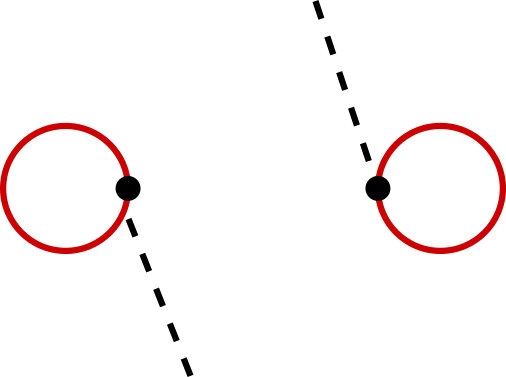
\includegraphics[scale=1]{figure/li_property_1.png}}%
%             \only<2>{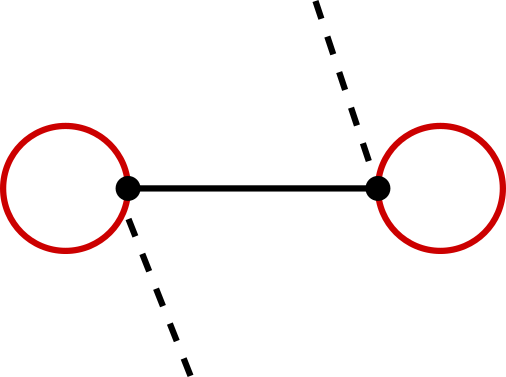
\includegraphics[scale=1]{figure/chap5-step1.png}}%
%         \end{center}

% \end{frame}


% \begin{frame}{Large Item sizes: Property 2-one isolated vertex and disjoint cycles}
%     Suppose $S \subseteq V$ such that $S = \{i \in V \mid x^{*}_{p_{i,1}} > 0 \ \text{or} \ x^{*}_{p_{i,2}} > 0\}$.
    
%     \begin{itemize}
%         \item  Recall that $x^*_p < 1 \ \forall p \in \mathcal{P}$, hence $\forall j \notin S$ we have,
            
%             \[1 = b_j = \sum_{i \in \delta(j)} x^*(p_{\{i,j\}}) < \sum_{i \in \delta(j)} 1 = |\delta(j)| \implies |\delta(j)| \geq 2 \; \forall j \notin S\] 
            
%         \item  By simple graph property,
%         \begin{equation*}
%             |E| = \frac{1}{2} \sum_{i=1}^{n} |\delta(i)| \geq \frac{1}{2} (2n - 2|S|) = n - |S|.
%         \end{equation*}
        
%         \item  Since $|E| = |\text{supp}(x^*)| - |S| \leq n - |S|$, there must be an equality. 
%             $\implies$ inequalities $|\delta(i)| \geq 0 \ \forall i \in S$ and $|\delta(j)| \geq 2  \ \forall j \notin S$ are also satisfied with equality.
            
%         \item  $\forall i \in V$ with $x^{*}_{p_{i,1}} > 0$ are isolated in $G \implies x^{*}_{p_{i,1}} = 1$ (\a{omitted due to residual instance}).
            
%     \end{itemize}
% \end{frame}


% \begin{frame}{Large Item sizes: Property 3-no even cycle}
%     Let $e_1,\ldots,e_{2k}$ be the edges of an even cycle such that $e_i \cap e_{i+1} \neq \varnothing \; \forall i \in\: [2k-1]$ and $e_1 \cap e_{2k} \neq \varnothing$.
    
%     \begin{itemize}
%         \item  Assume $x^*_{p_{{e}_1}} = \min_{i \in [2k]} x^*(p_{{e}_i})$.
        
%         \item  Modify $x^*$ to $\overline{x}^*$:
        
%             \[
%                 \overline{x}^*_p = \begin{cases}
%                     x^{*}_{p_{e_{2i}}} - x^{*}_{p_{e_{1}}}, & \text{for all $p_{e_{2i}}$} \\
%                     x^{*}_{p_{e_{2i+1}}} + x^{*}_{p_{e_{1}}}, & \text{for all $p_{e_{2i+1}}$} \\
%                     {x}^*_p, & \text{otherwise}
%                 \end{cases}
%              \]
             
%         \item  Since $\overline{x}^*_{p_{e_{1}}} = 0$, no even cycle.
%     \end{itemize}
% \end{frame}


% \begin{frame}{Large Item sizes: Property 4-odd cycle edge is half}
%     Let $e_1,\ldots,e_{2k+1}$ be the edges of an odd cycle.
    
%     \begin{itemize}
%         \item  It follows that $\forall i \in [2k]$, $x^*_{p_{{e}_i}} + x^*_{p_{{e}_{i+1}}} = 1$.
%         $\implies \forall i \in [k], x^*_{p_{{e}_1}} = x^*_{p_{{e}_{2i+1}}} \implies x^*_{p_{{e}_1}} = x^*_{p_{{e}_{2k+1}}}$.
        
%         \item  But $x^*_{p_{{e}_1}}$ and $x^*_{p_{{e}_{2k+1}}}$ are incident to one vertex.
        
%         $\implies \forall e \in C: x^*_{p_{{e}}} = \frac{1}{2}$.
        
%         \item  \textbf{\b{Claim}:} $\exists$ an edge $e = \{i,j\} \in C$ with $s_i \leq \frac{1}{2}$ and $s_j \leq \frac{1}{2}$.
        
%         \begin{center}
%             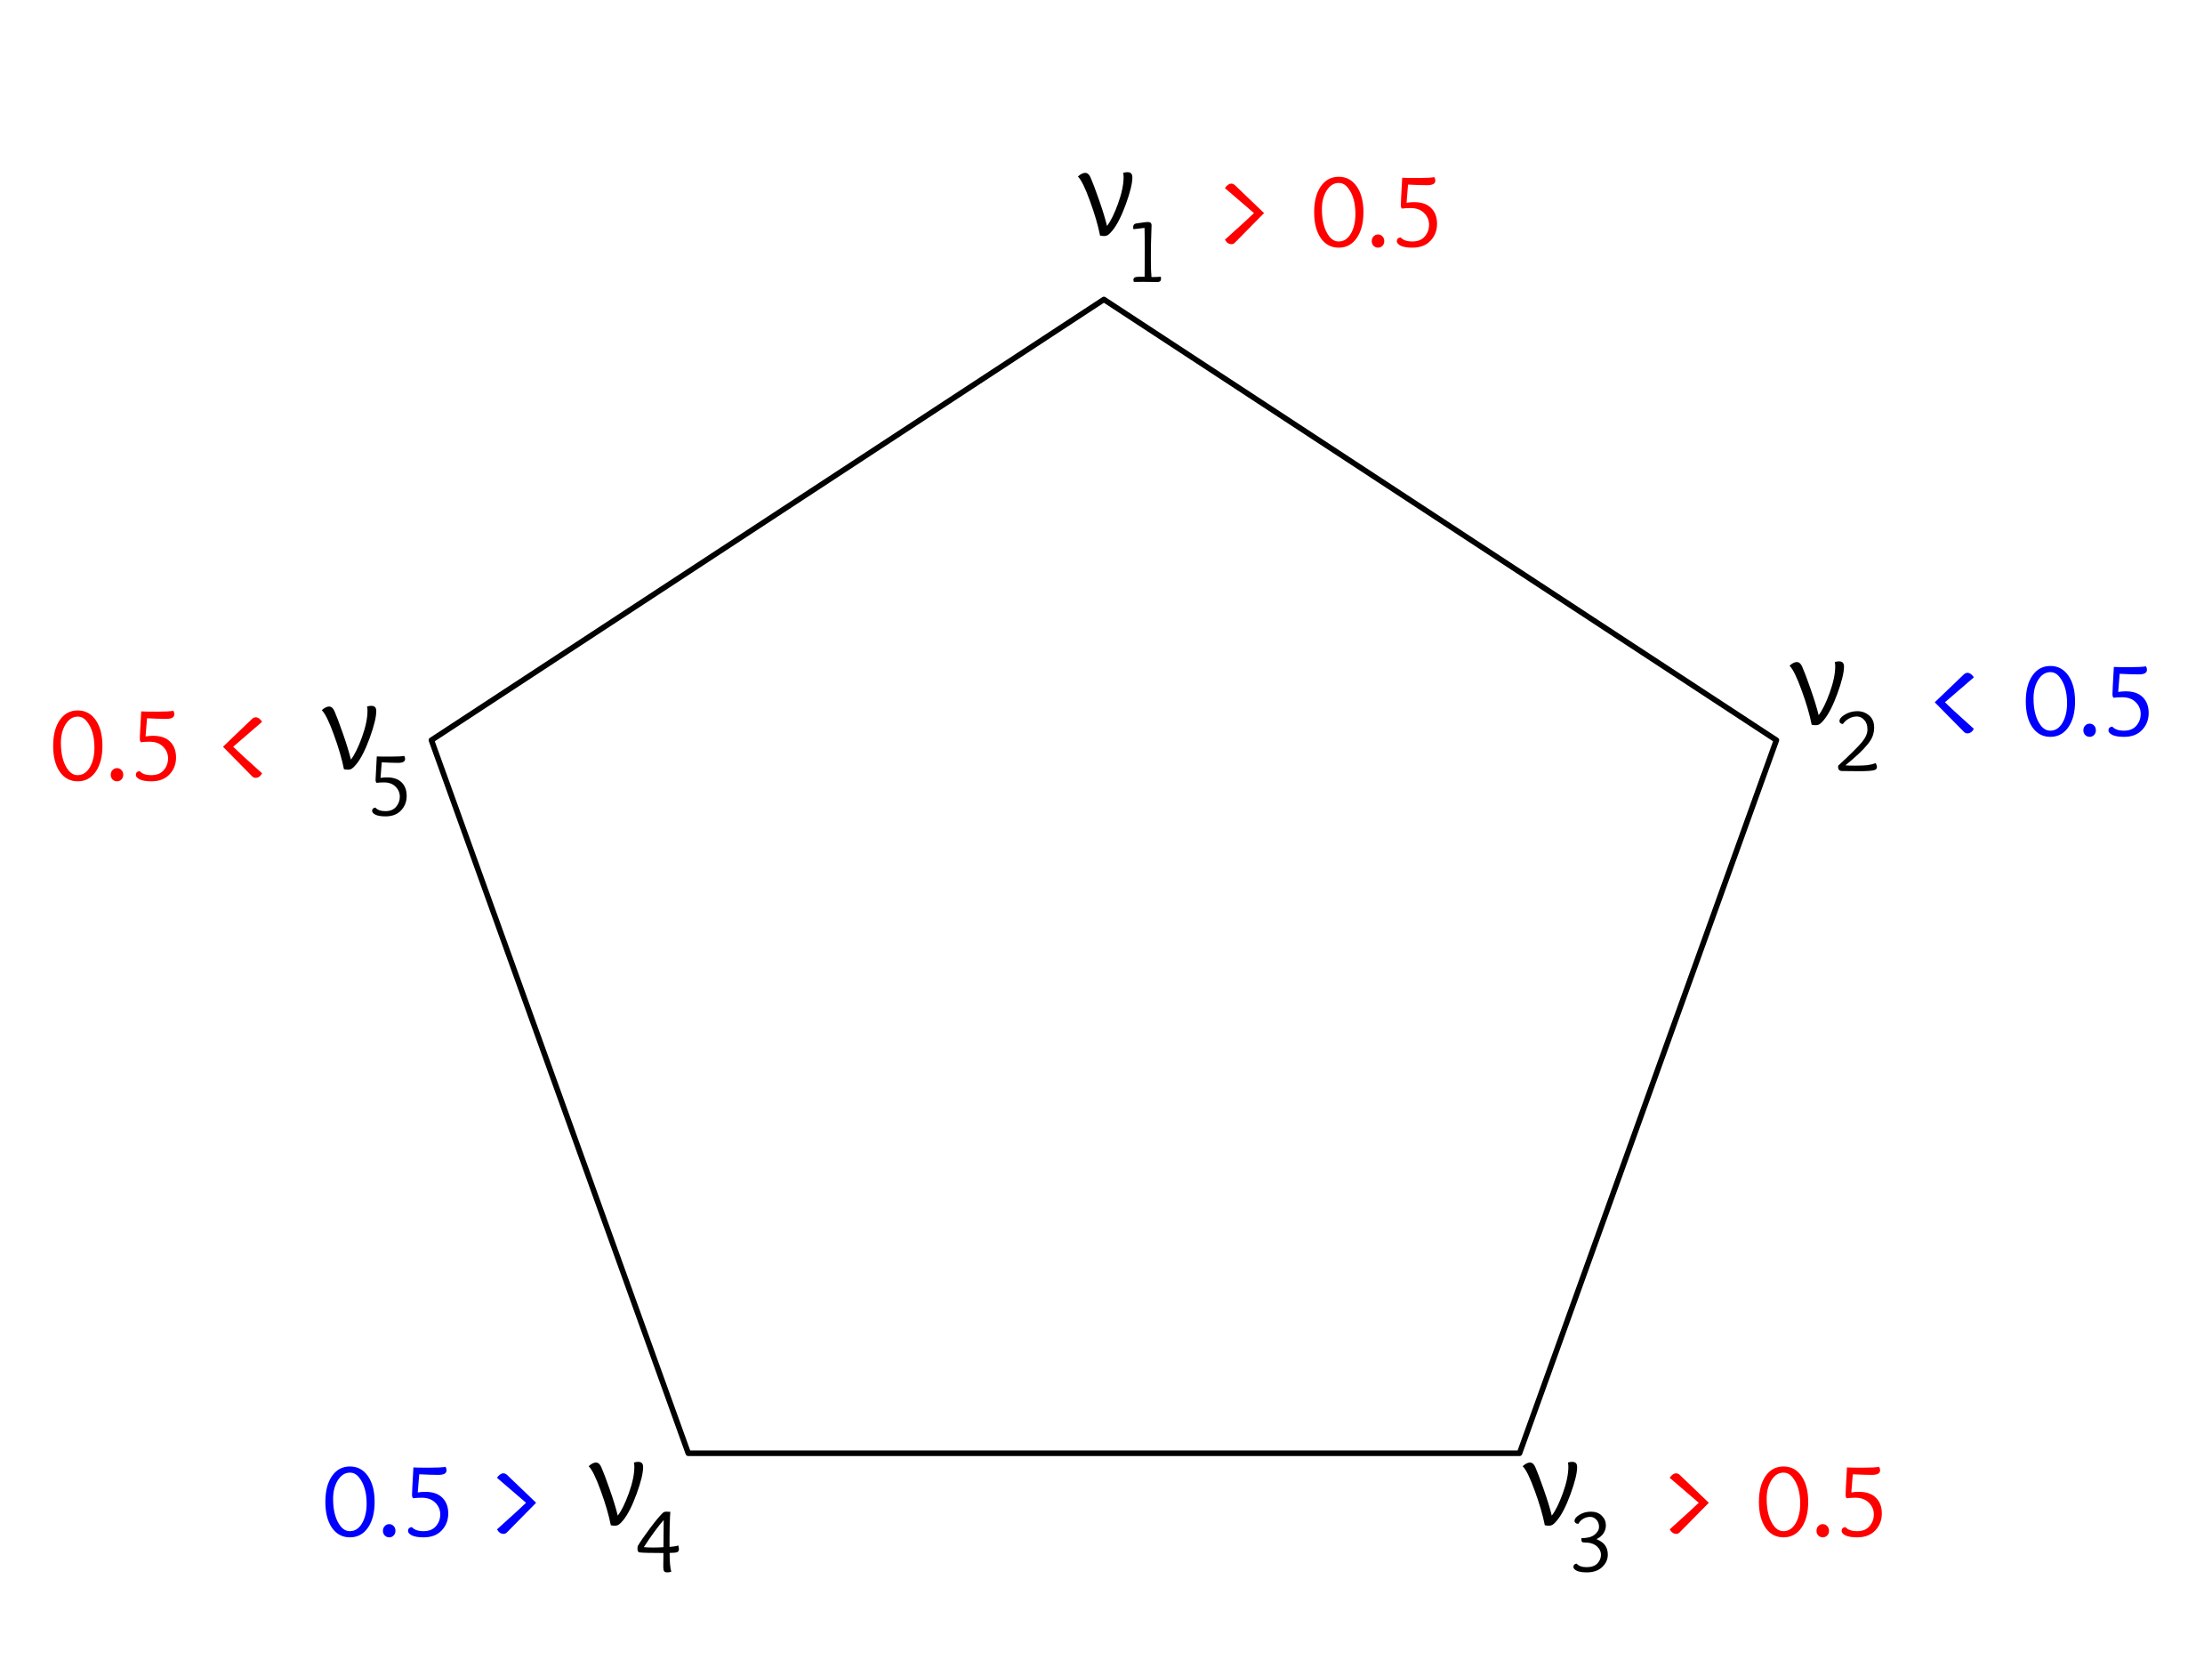
\includegraphics[scale=0.4]{figure/li_property_4_all_v_google.png}
%         \end{center}
%     \end{itemize}
    
% \end{frame}


% \begin{frame}{Large Item sizes: Property 5-at most one odd cycle}
%     \onslide<1>{Suppose $G$ has two cycles $C$ and $C'$ of odd length with edges $e_1,\ldots,e_{2k+1}$ and $e'_1,\ldots,e'_{2l+1}$.}
    
%     \begin{itemize}
%         \onslide<2>{\item From Property 4, we have that $x^*_{p_{e}} = x^*_{p_{e'}} =\frac{1}{2} \ \forall e \in C$ and $e' \in C'$.} 
        
%         \onslide<3>{\item Moreover, there exists $e =\{i,j\} \in C$ and $e' =\{i',j'\} \in C'$ such that $s_i, s_j, s_{i'}, s_{j'} \leq \frac{1}{2}$.} 
        
%             \onslide<4>{$\implies p_{\{i,i'\}}$ and $p_{\{j,j'\}}$ are feasible patterns.}
        
%         \onslide<5>{\item Modify $x^*$ to $x^*_p$ as 
        
%                 \[
%                     \overline{x}^*_p = \begin{cases}
%                     \frac{1}{2}, & \text{for all $p_{i,i'}$} \\
%                     \frac{1}{2}, & \text{for all $p_{j,j'}$} \\
%                     0, & \text{for all $p_e$}\\
%                     0, & \text{for all $p_{e'}$}\\
%                     {x}^*_p, & \text{otherwise}
%                     \end{cases}
%                 \]}
%     \end{itemize}
    
%             \begin{center}
%             \only<1-3>{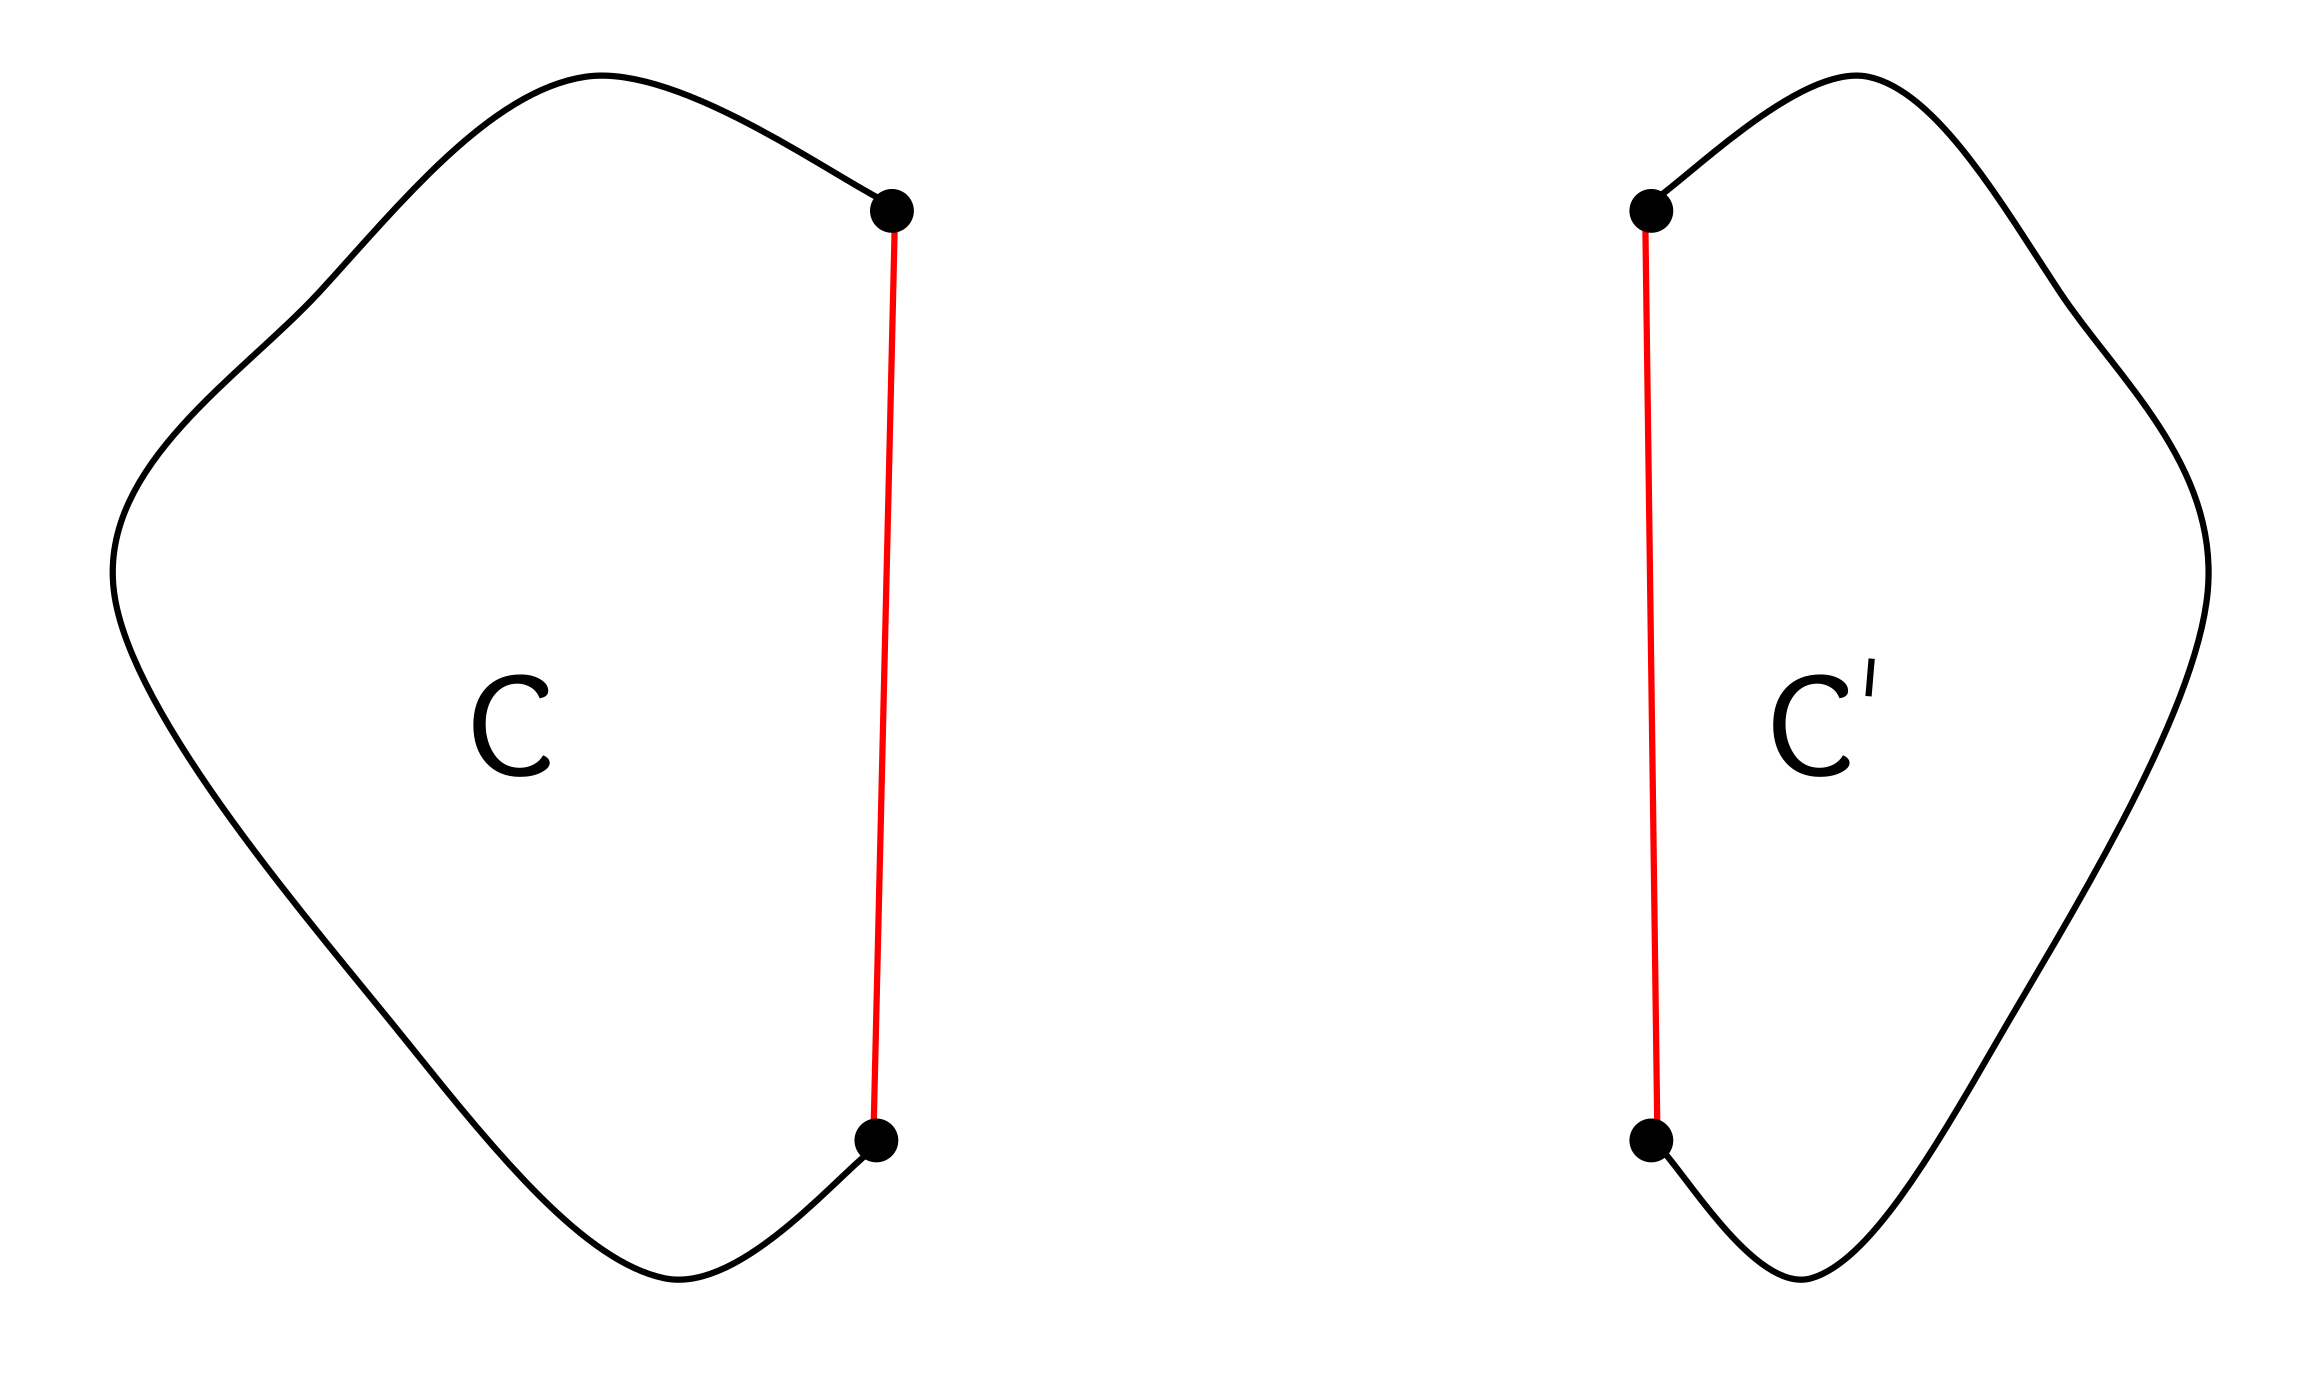
\includegraphics[scale=0.5]{figure/li_property_5_odd_cycle_1.png}}%
%             \only<4-5>{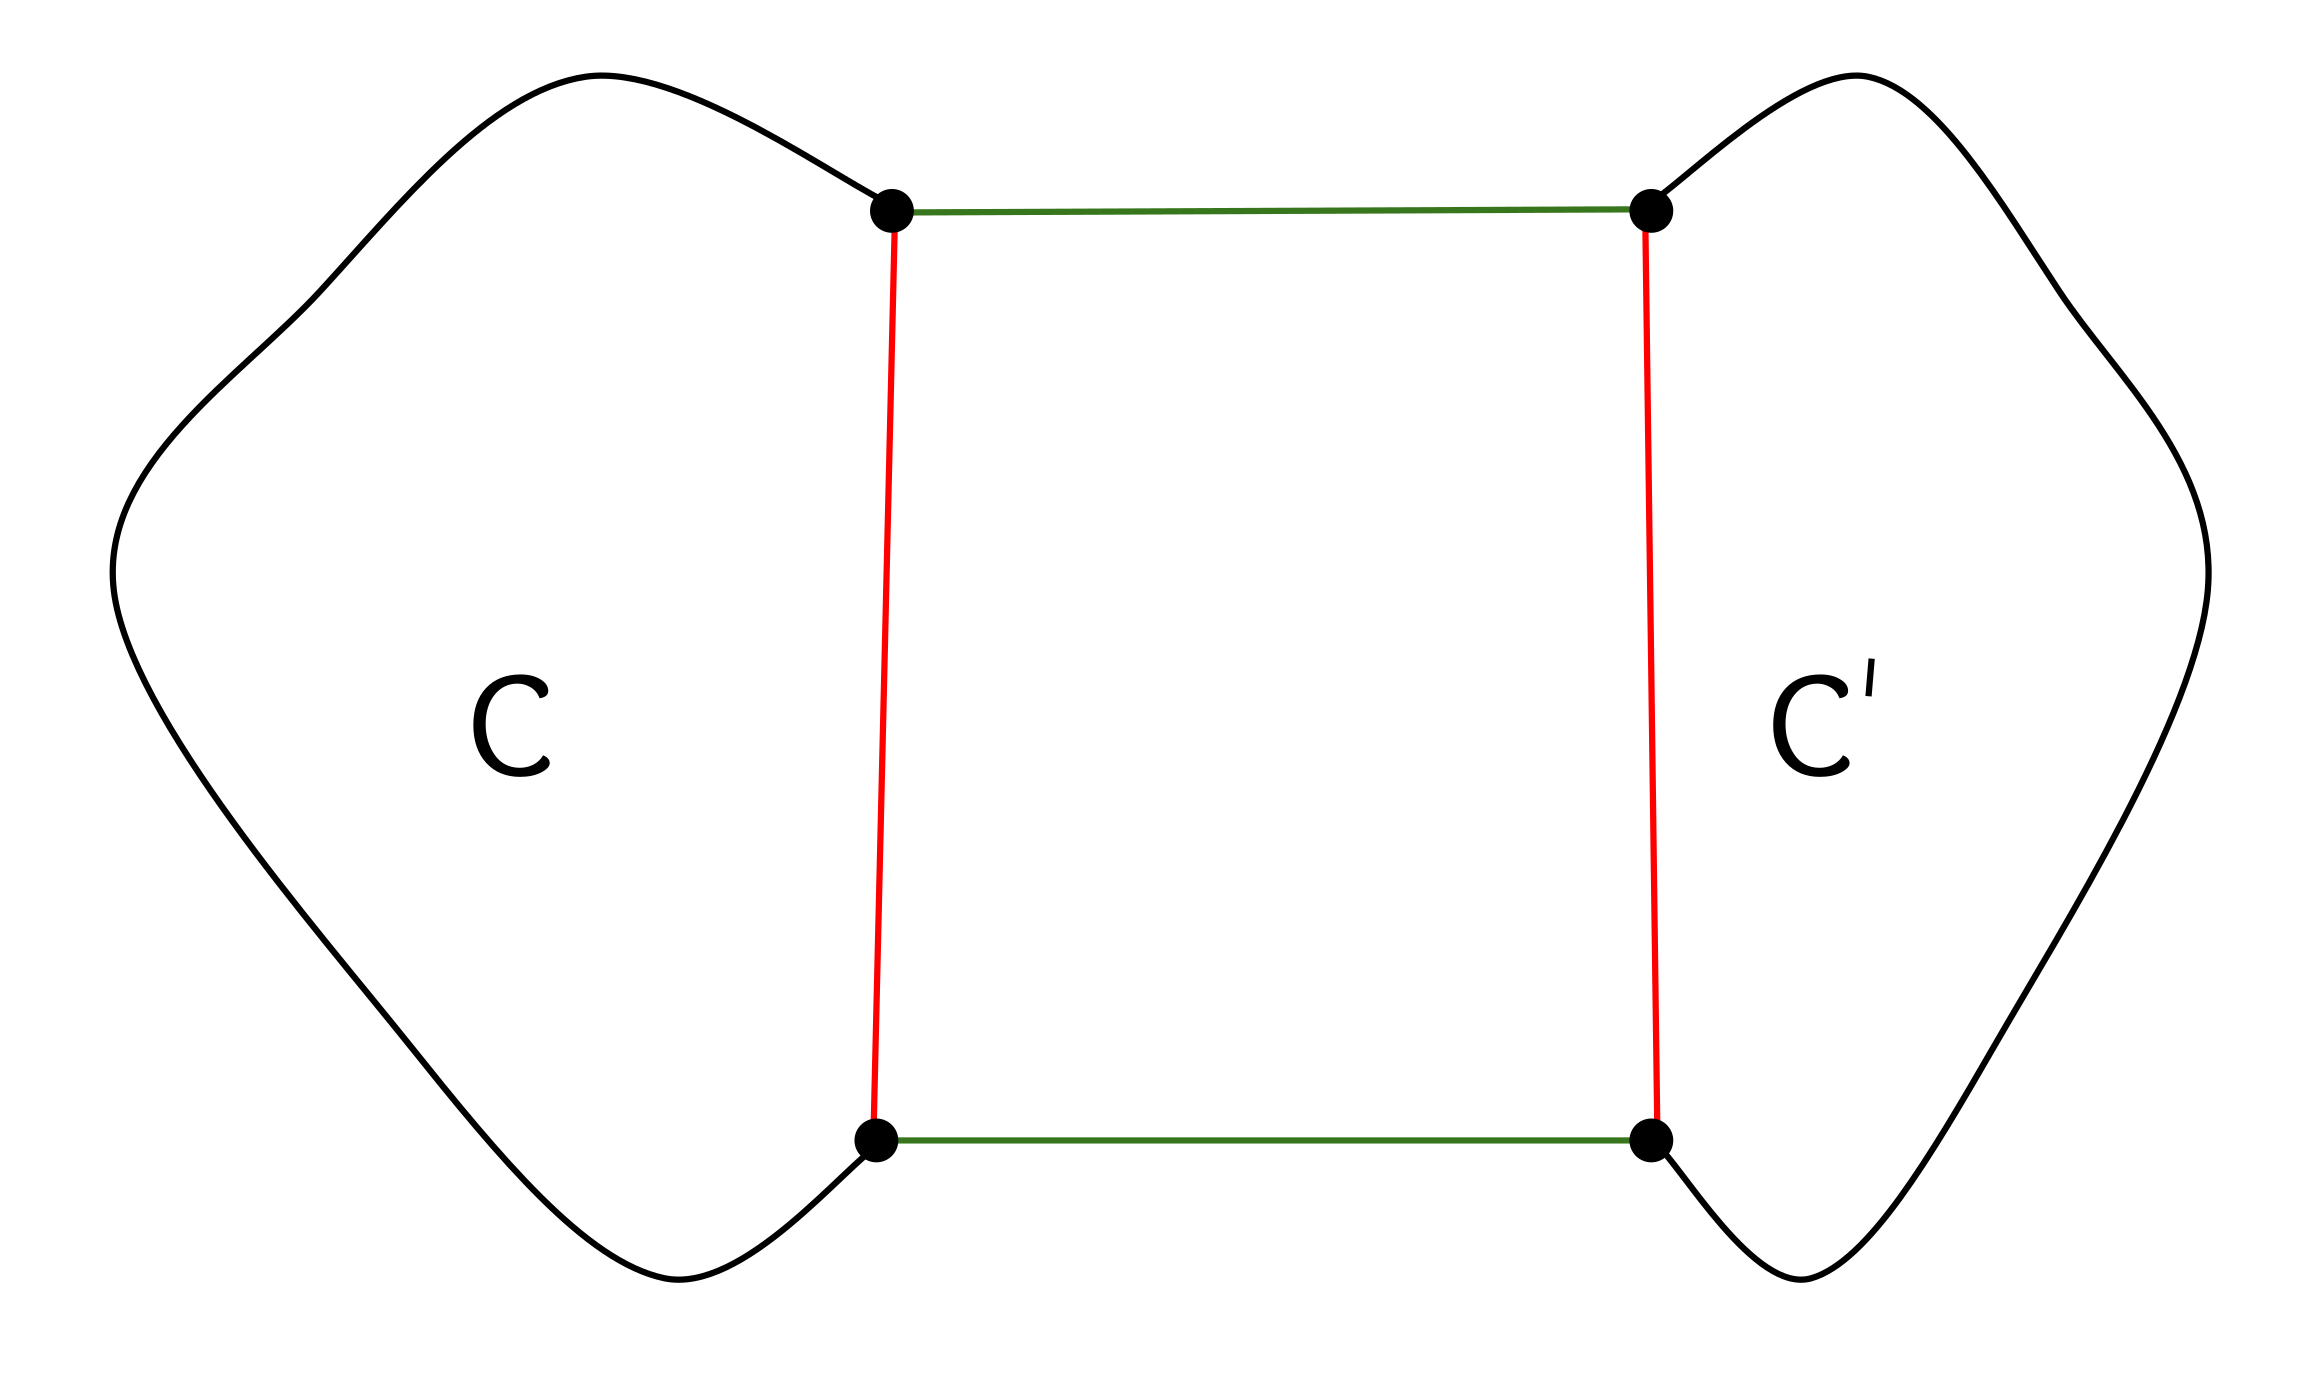
\includegraphics[scale=0.5]{figure/li_property_5_odd_cycle_final.png}}%
%         \end{center}
% \end{frame}


% \begin{frame}{Large Item sizes: Property 6-one odd cycle or one isolated vertex}

% Let $G$ consist of an isolated vertex $i$ and an odd cycle $C$ and there exists an edge $e = \{v,w\}$ s.t. $s_v, s_w \leq \frac{1}{2}$. 

%     \begin{itemize}
%         \item $i$ is an isolated vertex $\implies x^*(p_{i,2}) = \frac{1}{2}$, and $s_i \leq \frac{1}{2}$ as $p_{i,2}$ is a feasible pattern.
        
%         \item $p_{v,i}$ and $p_{w,i}$ are feasible patterns and modify $x^*$ to $\overline{x}^*_p$ as
        
%              \[
%                 \overline{x}^*_p = \begin{cases}
%                 \frac{1}{2}, & \text{for all $p_{\{v,i\}}$} \\
%                 \frac{1}{2}, & \text{for all $p_{\{w,i\}}$} \\
%                 0, & \text{for all $p_{v,2}$}\\
%                 {x}^*_p, & \text{otherwise}
%                 \end{cases}
%              \]

%     \end{itemize}
        
%         \begin{center}
%             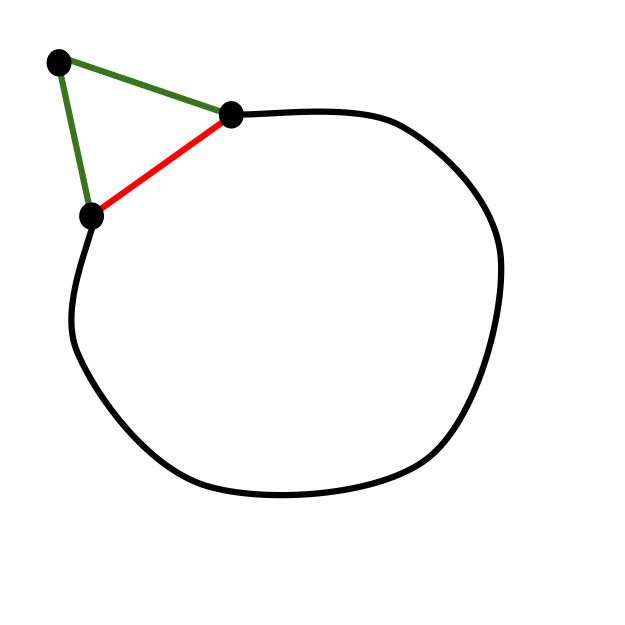
\includegraphics[scale=0.75]{figure/li_property_6_final.png}
%         \end{center}
% \end{frame}
\subsection{MIRUP Property of Instances with 7 different items}

\begin{frame}{Special instances adhering to MIRUP conjecture: $n \leq 7$}
    
    \onslide<1->{\begin{alertblock}{Theorem~\cite{nitsche1998new}}
        For all instances $I = (\a{6},s,b)$, $\mathsf{OPT}(I) \leq \lceil \mathsf{OPT_f}(I) \rceil + 1$.
    \end{alertblock}}
    
    \onslide<2->{Recall that,
    \begin{equation*}
        \begin{aligned}
        & & & \a{\text{Residual instance}} \implies \mathsf{OPT}(I) \leq n \\
        & & & \a{\text{Small items deleted}} \implies s_i > \frac{1}{\text{size}(I)} = \frac{1}{s^T \ b} \geq \frac{1}{\mathsf{OPT}(I)} \geq \frac{1}{n}
        \end{aligned}
    \end{equation*}}
\end{frame}

\begin{frame}{Special instances adhering to MIRUP conjecture: $n \leq 7$}

    \onslide<1->{\begin{theorem}
        For all instances $I = (\a{7},s,b)$, $\mathsf{OPT}(I) \leq \lceil \mathsf{OPT_f}(I) \rceil + 1$.
    \end{theorem}}
    
    \onslide<2->{\textbf{Proof.} Suppose optimum solution $\mathsf{OPT}(I) = m+2$ with the smallest item $s_s$ in the last bin.} 
    \onslide<3->{By employing LP duality, we construct a modified instance $I'$ such that $size(I')$ is maximized. That is, \vspace{0.2cm}
    
    Assign \a{weights} $w_1, w_2, \ldots, w_n$ such that:}
    
    \begin{itemize}
        
        \item<4->  $w^{\text{T}} \ p \leq 1 \ \text{wherever} \ s^{\text{T}} \ p \leq 1$.
                
                $\implies$ \emph{"patterns remains patterns"} \\
                $\implies \mathsf{OPT_f}(I') \geq \mathsf{OPT}(I)$ (Property of Duality)
        
        \item<5->  $size(I') = w^{\text{T}} \ b > m \implies$ \a{MIRUP instance} ($size(I') \leq \mathsf{OPT_f}(I')$) \QEDA
        
    \end{itemize}
    
\end{frame}


\begin{frame}{Special instances adhering to MIRUP conjecture: $n \leq 7$}

    % \textbf{Remark 1.} $s_i \geq \frac{1}{m-1}$ and all bins contain at most $m-2$ items. \newline
    % \textbf{Remark 2.} All $(m-2)$-bins are packed according to FFD heuristic. \QEDA
    
    \onslide<1->{\textbf{Example for $\mathsf{OPT_f} = 4$:} \newline
    By \a{\emph{residual instances}:} need to verify if $\lceil \mathsf{OPT_f}(I) \rceil = 1,2,3,4,5,6,7$ \vspace{0.2cm}}
    
    \onslide<2->{By \a{\emph{small items}:} all sizes $s_i > \frac{1}{3}$ \vspace{0.2cm}}
    
    \onslide<3->{\b{Optimum solution:} $\mathsf{OPT}(I) = p_1 + p_2 + p_3 + p_4 + \mathsf{R}$}
    
    \begin{itemize}
        \item<3-> either $\norm[]{p_i}_1 = 1$ or $\norm[]{p_i}_1 = 2$.
        
        \item<3-> $\norm[]{\mathsf{R}}_1 = 3$ and it contains the \a{smallest item}.
    \end{itemize}
    
    \onslide<4->{\b{Weights:}}
        \begin{itemize}
            \item<4->  \a{1} to 1-bins.
            \item<4->  \a{$\frac{1}{2}$} to 2-bins and largest item in $\mathsf{R}$.
        \end{itemize}

\end{frame}


\section{Discrepancy Theory Inspired Instances}

\begin{frame}{Beck's Conjecture}
    
    \begin{alertblock}{Beck's 3-permutation Conjecture}
        Given any \b{\emph{three permutations}} on $m$ elements, one can always find a color assignment such that in every interval of each of those permutations, the number of red and blue colored elements differ by a constant.
    \end{alertblock}
  
\only<2>{  
\begin{table}[]
\centering
\hskip-0.9cm
\small
{\renewcommand{\arraystretch}{0.8}
\begin{tabular}{ccccccccccccccccc}
{\color[HTML]{000000} permutation 1:} & {\color[HTML]{000000} } & \cellcolor[HTML]{C0C0C0}{\color[HTML]{000000} \begin{tabular}[c]{@{}l@{}}4\\ \statcirc{gray}\end{tabular}} & \cellcolor[HTML]{C0C0C0}{\color[HTML]{000000} } & \cellcolor[HTML]{C0C0C0}{\color[HTML]{000000} \begin{tabular}[c]{@{}l@{}}6\\ \statcirc{gray}\end{tabular}} & \cellcolor[HTML]{C0C0C0}{\color[HTML]{000000} } & \cellcolor[HTML]{C0C0C0}{\color[HTML]{000000} \begin{tabular}[c]{@{}l@{}}1\\ \statcirc{gray}\end{tabular}} & \cellcolor[HTML]{C0C0C0}{\color[HTML]{000000} } & \cellcolor[HTML]{C0C0C0}{\color[HTML]{000000} \begin{tabular}[c]{@{}l@{}}5\\ \statcirc{gray}\end{tabular}} & \cellcolor[HTML]{C0C0C0}{\color[HTML]{000000} } & \cellcolor[HTML]{C0C0C0}{\color[HTML]{000000} \begin{tabular}[c]{@{}l@{}}7\\ \statcirc{gray}\end{tabular}} & \cellcolor[HTML]{C0C0C0}{\color[HTML]{000000} } & \cellcolor[HTML]{C0C0C0}{\color[HTML]{000000} \begin{tabular}[c]{@{}l@{}}2\\ \statcirc{gray}\end{tabular}} & \cellcolor[HTML]{C0C0C0}{\color[HTML]{000000} } & \cellcolor[HTML]{C0C0C0}{\color[HTML]{000000} \begin{tabular}[c]{@{}l@{}}8\\ \statcirc{gray}\end{tabular}} & \cellcolor[HTML]{C0C0C0}{\color[HTML]{000000} } & \cellcolor[HTML]{C0C0C0}{\color[HTML]{000000} \begin{tabular}[c]{@{}l@{}}3\\ \statcirc{gray}\end{tabular}} \\
{\color[HTML]{000000} } & {\color[HTML]{000000} } & {\color[HTML]{000000} } & {\color[HTML]{000000} } & {\color[HTML]{000000} } & {\color[HTML]{000000} } & {\color[HTML]{000000} } & {\color[HTML]{000000} } & {\color[HTML]{000000} } & {\color[HTML]{000000} } & {\color[HTML]{000000} } & {\color[HTML]{000000} } & {\color[HTML]{000000} } & {\color[HTML]{000000} } & {\color[HTML]{000000} } & {\color[HTML]{000000} } & {\color[HTML]{000000} } \\
{\color[HTML]{000000} permutation 2:} & {\color[HTML]{000000} } & \cellcolor[HTML]{C0C0C0}{\color[HTML]{000000} \begin{tabular}[c]{@{}l@{}}7\\ \statcirc{gray}\end{tabular}} & \cellcolor[HTML]{C0C0C0}{\color[HTML]{000000} } & \cellcolor[HTML]{C0C0C0}{\color[HTML]{000000} \begin{tabular}[c]{@{}l@{}}8\\ \statcirc{gray}\end{tabular}} & \cellcolor[HTML]{C0C0C0}{\color[HTML]{000000} } & \cellcolor[HTML]{C0C0C0}{\color[HTML]{000000} \begin{tabular}[c]{@{}l@{}}2\\ \statcirc{gray}\end{tabular}} & \cellcolor[HTML]{C0C0C0}{\color[HTML]{000000} } & \cellcolor[HTML]{C0C0C0}{\color[HTML]{000000} \begin{tabular}[c]{@{}l@{}}5\\ \statcirc{gray}\end{tabular}} & \cellcolor[HTML]{C0C0C0}{\color[HTML]{000000} } & \cellcolor[HTML]{C0C0C0}{\color[HTML]{000000} \begin{tabular}[c]{@{}l@{}}3\\ \statcirc{gray}\end{tabular}} & \cellcolor[HTML]{C0C0C0}{\color[HTML]{000000} } & \cellcolor[HTML]{C0C0C0}{\color[HTML]{000000} \begin{tabular}[c]{@{}l@{}}4\\ \statcirc{gray}\end{tabular}} & \cellcolor[HTML]{C0C0C0}{\color[HTML]{000000} } & \cellcolor[HTML]{C0C0C0}{\color[HTML]{000000} \begin{tabular}[c]{@{}l@{}}1\\ \statcirc{gray}\end{tabular}} & \cellcolor[HTML]{C0C0C0}{\color[HTML]{000000} } & \cellcolor[HTML]{C0C0C0}{\color[HTML]{000000} \begin{tabular}[c]{@{}l@{}}6\\ \statcirc{gray}\end{tabular}} \\
{\color[HTML]{000000} } & {\color[HTML]{000000} } & {\color[HTML]{000000} } & {\color[HTML]{000000} } & {\color[HTML]{000000} } & {\color[HTML]{000000} } & {\color[HTML]{000000} } & {\color[HTML]{000000} } & {\color[HTML]{000000} } & {\color[HTML]{000000} } & {\color[HTML]{000000} } & {\color[HTML]{000000} } & {\color[HTML]{000000} } & {\color[HTML]{000000} } & {\color[HTML]{000000} } & {\color[HTML]{000000} } & {\color[HTML]{000000} } \\
{\color[HTML]{000000} permutation 3:} & {\color[HTML]{000000} } & \cellcolor[HTML]{C0C0C0}{\color[HTML]{000000} \begin{tabular}[c]{@{}l@{}}2\\ \statcirc{gray}\end{tabular}} & \cellcolor[HTML]{C0C0C0}{\color[HTML]{000000} } & \cellcolor[HTML]{C0C0C0}{\color[HTML]{000000} \begin{tabular}[c]{@{}l@{}}1\\ \statcirc{gray}\end{tabular}} & \cellcolor[HTML]{C0C0C0}{\color[HTML]{000000} } & \cellcolor[HTML]{C0C0C0}{\color[HTML]{000000} \begin{tabular}[c]{@{}l@{}}6\\ \statcirc{gray}\end{tabular}} & \cellcolor[HTML]{C0C0C0}{\color[HTML]{000000} } & \cellcolor[HTML]{C0C0C0}{\color[HTML]{000000} \begin{tabular}[c]{@{}l@{}}4\\ \statcirc{gray}\end{tabular}} & \cellcolor[HTML]{C0C0C0}{\color[HTML]{000000} } & \cellcolor[HTML]{C0C0C0}{\color[HTML]{000000} \begin{tabular}[c]{@{}l@{}}8\\ \statcirc{gray}\end{tabular}} & \cellcolor[HTML]{C0C0C0}{\color[HTML]{000000} } & \cellcolor[HTML]{C0C0C0}{\color[HTML]{000000} \begin{tabular}[c]{@{}l@{}}5\\ \statcirc{gray}\end{tabular}} & \cellcolor[HTML]{C0C0C0}{\color[HTML]{000000} } & \cellcolor[HTML]{C0C0C0}{\color[HTML]{000000} \begin{tabular}[c]{@{}l@{}}3\\ \statcirc{gray}\end{tabular}} & \cellcolor[HTML]{C0C0C0}{\color[HTML]{000000} } & \cellcolor[HTML]{C0C0C0}{\color[HTML]{000000} \begin{tabular}[c]{@{}l@{}}7\\ \statcirc{gray}\end{tabular}}
\end{tabular}}
\end{table}
}

\only<3>{
\begin{table}[]
\centering
\hskip-0.9cm
\small
{\renewcommand{\arraystretch}{0.8}
\begin{tabular}{ccccccccccccccccc}
{\color[HTML]{000000} permutation 1:} & {\color[HTML]{000000} } & \cellcolor[HTML]{C0C0C0}{\color[HTML]{000000} \begin{tabular}[c]{@{}l@{}}4\\ \statcirc{gray}\end{tabular}} & \cellcolor[HTML]{C0C0C0}{\color[HTML]{000000} } & \cellcolor[HTML]{C0C0C0}{\color[HTML]{000000} \begin{tabular}[c]{@{}l@{}}6\\ \statcirc{gray}\end{tabular}} & \cellcolor[HTML]{C0C0C0}{\color[HTML]{000000} } & \cellcolor[HTML]{C0C0C0}{\color[HTML]{000000} \begin{tabular}[c]{@{}l@{}}1\\ \statcirc{red}\end{tabular}} & \cellcolor[HTML]{C0C0C0}{\color[HTML]{000000} } & \cellcolor[HTML]{C0C0C0}{\color[HTML]{000000} \begin{tabular}[c]{@{}l@{}}5\\ \statcirc{gray}\end{tabular}} & \cellcolor[HTML]{C0C0C0}{\color[HTML]{000000} } & \cellcolor[HTML]{C0C0C0}{\color[HTML]{000000} \begin{tabular}[c]{@{}l@{}}7\\ \statcirc{gray}\end{tabular}} & \cellcolor[HTML]{C0C0C0}{\color[HTML]{000000} } & \cellcolor[HTML]{C0C0C0}{\color[HTML]{000000} \begin{tabular}[c]{@{}l@{}}2\\ \statcirc{gray}\end{tabular}} & \cellcolor[HTML]{C0C0C0}{\color[HTML]{000000} } & \cellcolor[HTML]{C0C0C0}{\color[HTML]{000000} \begin{tabular}[c]{@{}l@{}}8\\ \statcirc{gray}\end{tabular}} & \cellcolor[HTML]{C0C0C0}{\color[HTML]{000000} } & \cellcolor[HTML]{C0C0C0}{\color[HTML]{000000} \begin{tabular}[c]{@{}l@{}}3\\ \statcirc{gray}\end{tabular}} \\
{\color[HTML]{000000} } & {\color[HTML]{000000} } & {\color[HTML]{000000} } & {\color[HTML]{000000} } & {\color[HTML]{000000} } & {\color[HTML]{000000} } & {\color[HTML]{000000} } & {\color[HTML]{000000} } & {\color[HTML]{000000} } & {\color[HTML]{000000} } & {\color[HTML]{000000} } & {\color[HTML]{000000} } & {\color[HTML]{000000} } & {\color[HTML]{000000} } & {\color[HTML]{000000} } & {\color[HTML]{000000} } & {\color[HTML]{000000} } \\
{\color[HTML]{000000} permutation 2:} & {\color[HTML]{000000} } & \cellcolor[HTML]{C0C0C0}{\color[HTML]{000000} \begin{tabular}[c]{@{}l@{}}7\\ \statcirc{gray}\end{tabular}} & \cellcolor[HTML]{C0C0C0}{\color[HTML]{000000} } & \cellcolor[HTML]{C0C0C0}{\color[HTML]{000000} \begin{tabular}[c]{@{}l@{}}8\\ \statcirc{gray}\end{tabular}} & \cellcolor[HTML]{C0C0C0}{\color[HTML]{000000} } & \cellcolor[HTML]{C0C0C0}{\color[HTML]{000000} \begin{tabular}[c]{@{}l@{}}2\\ \statcirc{gray}\end{tabular}} & \cellcolor[HTML]{C0C0C0}{\color[HTML]{000000} } & \cellcolor[HTML]{C0C0C0}{\color[HTML]{000000} \begin{tabular}[c]{@{}l@{}}5\\ \statcirc{gray}\end{tabular}} & \cellcolor[HTML]{C0C0C0}{\color[HTML]{000000} } & \cellcolor[HTML]{C0C0C0}{\color[HTML]{000000} \begin{tabular}[c]{@{}l@{}}3\\ \statcirc{gray}\end{tabular}} & \cellcolor[HTML]{C0C0C0}{\color[HTML]{000000} } & \cellcolor[HTML]{C0C0C0}{\color[HTML]{000000} \begin{tabular}[c]{@{}l@{}}4\\ \statcirc{gray}\end{tabular}} & \cellcolor[HTML]{C0C0C0}{\color[HTML]{000000} } & \cellcolor[HTML]{C0C0C0}{\color[HTML]{000000} \begin{tabular}[c]{@{}l@{}}1\\ \statcirc{red}\end{tabular}} & \cellcolor[HTML]{C0C0C0}{\color[HTML]{000000} } & \cellcolor[HTML]{C0C0C0}{\color[HTML]{000000} \begin{tabular}[c]{@{}l@{}}6\\ \statcirc{gray}\end{tabular}} \\
{\color[HTML]{000000} } & {\color[HTML]{000000} } & {\color[HTML]{000000} } & {\color[HTML]{000000} } & {\color[HTML]{000000} } & {\color[HTML]{000000} } & {\color[HTML]{000000} } & {\color[HTML]{000000} } & {\color[HTML]{000000} } & {\color[HTML]{000000} } & {\color[HTML]{000000} } & {\color[HTML]{000000} } & {\color[HTML]{000000} } & {\color[HTML]{000000} } & {\color[HTML]{000000} } & {\color[HTML]{000000} } & {\color[HTML]{000000} } \\
{\color[HTML]{000000} permutation 3:} & {\color[HTML]{000000} } & \cellcolor[HTML]{C0C0C0}{\color[HTML]{000000} \begin{tabular}[c]{@{}l@{}}2\\ \statcirc{gray}\end{tabular}} & \cellcolor[HTML]{C0C0C0}{\color[HTML]{000000} } & \cellcolor[HTML]{C0C0C0}{\color[HTML]{000000} \begin{tabular}[c]{@{}l@{}}1\\ \statcirc{red}\end{tabular}} & \cellcolor[HTML]{C0C0C0}{\color[HTML]{000000} } & \cellcolor[HTML]{C0C0C0}{\color[HTML]{000000} \begin{tabular}[c]{@{}l@{}}6\\ \statcirc{gray}\end{tabular}} & \cellcolor[HTML]{C0C0C0}{\color[HTML]{000000} } & \cellcolor[HTML]{C0C0C0}{\color[HTML]{000000} \begin{tabular}[c]{@{}l@{}}4\\ \statcirc{gray}\end{tabular}} & \cellcolor[HTML]{C0C0C0}{\color[HTML]{000000} } & \cellcolor[HTML]{C0C0C0}{\color[HTML]{000000} \begin{tabular}[c]{@{}l@{}}8\\ \statcirc{gray}\end{tabular}} & \cellcolor[HTML]{C0C0C0}{\color[HTML]{000000} } & \cellcolor[HTML]{C0C0C0}{\color[HTML]{000000} \begin{tabular}[c]{@{}l@{}}5\\ \statcirc{gray}\end{tabular}} & \cellcolor[HTML]{C0C0C0}{\color[HTML]{000000} } & \cellcolor[HTML]{C0C0C0}{\color[HTML]{000000} \begin{tabular}[c]{@{}l@{}}3\\ \statcirc{gray}\end{tabular}} & \cellcolor[HTML]{C0C0C0}{\color[HTML]{000000} } & \cellcolor[HTML]{C0C0C0}{\color[HTML]{000000} \begin{tabular}[c]{@{}l@{}}7\\ \statcirc{gray}\end{tabular}}
\end{tabular}}
\end{table}
}

\only<4>{
\begin{table}[]
\centering
\hskip-0.9cm
\small
{\renewcommand{\arraystretch}{0.8}
\begin{tabular}{ccccccccccccccccc}
{\color[HTML]{000000} permutation 1:} & {\color[HTML]{000000} } & \cellcolor[HTML]{C0C0C0}{\color[HTML]{000000} \begin{tabular}[c]{@{}l@{}}4\\ \statcirc{gray}\end{tabular}} & \cellcolor[HTML]{C0C0C0}{\color[HTML]{000000} } & \cellcolor[HTML]{C0C0C0}{\color[HTML]{000000} \begin{tabular}[c]{@{}l@{}}6\\ \statcirc{gray}\end{tabular}} & \cellcolor[HTML]{C0C0C0}{\color[HTML]{000000} } & \cellcolor[HTML]{C0C0C0}{\color[HTML]{000000} \begin{tabular}[c]{@{}l@{}}1\\ \statcirc{red}\end{tabular}} & \cellcolor[HTML]{C0C0C0}{\color[HTML]{000000} } & \cellcolor[HTML]{C0C0C0}{\color[HTML]{000000} \begin{tabular}[c]{@{}l@{}}5\\ \statcirc{gray}\end{tabular}} & \cellcolor[HTML]{C0C0C0}{\color[HTML]{000000} } & \cellcolor[HTML]{C0C0C0}{\color[HTML]{000000} \begin{tabular}[c]{@{}l@{}}7\\ \statcirc{gray}\end{tabular}} & \cellcolor[HTML]{C0C0C0}{\color[HTML]{000000} } & \cellcolor[HTML]{C0C0C0}{\color[HTML]{000000} \begin{tabular}[c]{@{}l@{}}2\\ \statcirc{blue}\end{tabular}} & \cellcolor[HTML]{C0C0C0}{\color[HTML]{000000} } & \cellcolor[HTML]{C0C0C0}{\color[HTML]{000000} \begin{tabular}[c]{@{}l@{}}8\\ \statcirc{gray}\end{tabular}} & \cellcolor[HTML]{C0C0C0}{\color[HTML]{000000} } & \cellcolor[HTML]{C0C0C0}{\color[HTML]{000000} \begin{tabular}[c]{@{}l@{}}3\\ \statcirc{gray}\end{tabular}} \\
{\color[HTML]{000000} } & {\color[HTML]{000000} } & {\color[HTML]{000000} } & {\color[HTML]{000000} } & {\color[HTML]{000000} } & {\color[HTML]{000000} } & {\color[HTML]{000000} } & {\color[HTML]{000000} } & {\color[HTML]{000000} } & {\color[HTML]{000000} } & {\color[HTML]{000000} } & {\color[HTML]{000000} } & {\color[HTML]{000000} } & {\color[HTML]{000000} } & {\color[HTML]{000000} } & {\color[HTML]{000000} } & {\color[HTML]{000000} } \\
{\color[HTML]{000000} permutation 2:} & {\color[HTML]{000000} } & \cellcolor[HTML]{C0C0C0}{\color[HTML]{000000} \begin{tabular}[c]{@{}l@{}}7\\ \statcirc{gray}\end{tabular}} & \cellcolor[HTML]{C0C0C0}{\color[HTML]{000000} } & \cellcolor[HTML]{C0C0C0}{\color[HTML]{000000} \begin{tabular}[c]{@{}l@{}}8\\ \statcirc{gray}\end{tabular}} & \cellcolor[HTML]{C0C0C0}{\color[HTML]{000000} } & \cellcolor[HTML]{C0C0C0}{\color[HTML]{000000} \begin{tabular}[c]{@{}l@{}}2\\ \statcirc{blue}\end{tabular}} & \cellcolor[HTML]{C0C0C0}{\color[HTML]{000000} } & \cellcolor[HTML]{C0C0C0}{\color[HTML]{000000} \begin{tabular}[c]{@{}l@{}}5\\ \statcirc{gray}\end{tabular}} & \cellcolor[HTML]{C0C0C0}{\color[HTML]{000000} } & \cellcolor[HTML]{C0C0C0}{\color[HTML]{000000} \begin{tabular}[c]{@{}l@{}}3\\ \statcirc{gray}\end{tabular}} & \cellcolor[HTML]{C0C0C0}{\color[HTML]{000000} } & \cellcolor[HTML]{C0C0C0}{\color[HTML]{000000} \begin{tabular}[c]{@{}l@{}}4\\ \statcirc{gray}\end{tabular}} & \cellcolor[HTML]{C0C0C0}{\color[HTML]{000000} } & \cellcolor[HTML]{C0C0C0}{\color[HTML]{000000} \begin{tabular}[c]{@{}l@{}}1\\ \statcirc{red}\end{tabular}} & \cellcolor[HTML]{C0C0C0}{\color[HTML]{000000} } & \cellcolor[HTML]{C0C0C0}{\color[HTML]{000000} \begin{tabular}[c]{@{}l@{}}6\\ \statcirc{gray}\end{tabular}} \\
{\color[HTML]{000000} } & {\color[HTML]{000000} } & {\color[HTML]{000000} } & {\color[HTML]{000000} } & {\color[HTML]{000000} } & {\color[HTML]{000000} } & {\color[HTML]{000000} } & {\color[HTML]{000000} } & {\color[HTML]{000000} } & {\color[HTML]{000000} } & {\color[HTML]{000000} } & {\color[HTML]{000000} } & {\color[HTML]{000000} } & {\color[HTML]{000000} } & {\color[HTML]{000000} } & {\color[HTML]{000000} } & {\color[HTML]{000000} } \\
{\color[HTML]{000000} permutation 3:} & {\color[HTML]{000000} } & \cellcolor[HTML]{C0C0C0}{\color[HTML]{000000} \begin{tabular}[c]{@{}l@{}}2\\ \statcirc{blue}\end{tabular}} & \cellcolor[HTML]{C0C0C0}{\color[HTML]{000000} } & \cellcolor[HTML]{C0C0C0}{\color[HTML]{000000} \begin{tabular}[c]{@{}l@{}}1\\ \statcirc{red}\end{tabular}} & \cellcolor[HTML]{C0C0C0}{\color[HTML]{000000} } & \cellcolor[HTML]{C0C0C0}{\color[HTML]{000000} \begin{tabular}[c]{@{}l@{}}6\\ \statcirc{gray}\end{tabular}} & \cellcolor[HTML]{C0C0C0}{\color[HTML]{000000} } & \cellcolor[HTML]{C0C0C0}{\color[HTML]{000000} \begin{tabular}[c]{@{}l@{}}4\\ \statcirc{gray}\end{tabular}} & \cellcolor[HTML]{C0C0C0}{\color[HTML]{000000} } & \cellcolor[HTML]{C0C0C0}{\color[HTML]{000000} \begin{tabular}[c]{@{}l@{}}8\\ \statcirc{gray}\end{tabular}} & \cellcolor[HTML]{C0C0C0}{\color[HTML]{000000} } & \cellcolor[HTML]{C0C0C0}{\color[HTML]{000000} \begin{tabular}[c]{@{}l@{}}5\\ \statcirc{gray}\end{tabular}} & \cellcolor[HTML]{C0C0C0}{\color[HTML]{000000} } & \cellcolor[HTML]{C0C0C0}{\color[HTML]{000000} \begin{tabular}[c]{@{}l@{}}3\\ \statcirc{gray}\end{tabular}} & \cellcolor[HTML]{C0C0C0}{\color[HTML]{000000} } & \cellcolor[HTML]{C0C0C0}{\color[HTML]{000000} \begin{tabular}[c]{@{}l@{}}7\\ \statcirc{gray}\end{tabular}}
\end{tabular}}
\end{table}
}

\only<5>{
\begin{table}[]
\centering
\hskip-0.9cm
\small
{\renewcommand{\arraystretch}{0.8}
\begin{tabular}{ccccccccccccccccc}
{\color[HTML]{000000} permutation 1:} & {\color[HTML]{000000} } & \cellcolor[HTML]{C0C0C0}{\color[HTML]{000000} \begin{tabular}[c]{@{}l@{}}4\\ \statcirc{gray}\end{tabular}} & \cellcolor[HTML]{C0C0C0}{\color[HTML]{000000} } & \cellcolor[HTML]{C0C0C0}{\color[HTML]{000000} \begin{tabular}[c]{@{}l@{}}6\\ \statcirc{gray}\end{tabular}} & \cellcolor[HTML]{C0C0C0}{\color[HTML]{000000} } & \cellcolor[HTML]{C0C0C0}{\color[HTML]{000000} \begin{tabular}[c]{@{}l@{}}1\\ \statcirc{red}\end{tabular}} & \cellcolor[HTML]{C0C0C0}{\color[HTML]{000000} } & \cellcolor[HTML]{C0C0C0}{\color[HTML]{000000} \begin{tabular}[c]{@{}l@{}}5\\ \statcirc{gray}\end{tabular}} & \cellcolor[HTML]{C0C0C0}{\color[HTML]{000000} } & \cellcolor[HTML]{C0C0C0}{\color[HTML]{000000} \begin{tabular}[c]{@{}l@{}}7\\ \statcirc{gray}\end{tabular}} & \cellcolor[HTML]{C0C0C0}{\color[HTML]{000000} } & \cellcolor[HTML]{C0C0C0}{\color[HTML]{000000} \begin{tabular}[c]{@{}l@{}}2\\ \statcirc{blue}\end{tabular}} & \cellcolor[HTML]{C0C0C0}{\color[HTML]{000000} } & \cellcolor[HTML]{C0C0C0}{\color[HTML]{000000} \begin{tabular}[c]{@{}l@{}}8\\ \statcirc{gray}\end{tabular}} & \cellcolor[HTML]{C0C0C0}{\color[HTML]{000000} } & \cellcolor[HTML]{C0C0C0}{\color[HTML]{000000} \begin{tabular}[c]{@{}l@{}}3\\ \statcirc{blue}\end{tabular}} \\
{\color[HTML]{000000} } & {\color[HTML]{000000} } & {\color[HTML]{000000} } & {\color[HTML]{000000} } & {\color[HTML]{000000} } & {\color[HTML]{000000} } & {\color[HTML]{000000} } & {\color[HTML]{000000} } & {\color[HTML]{000000} } & {\color[HTML]{000000} } & {\color[HTML]{000000} } & {\color[HTML]{000000} } & {\color[HTML]{000000} } & {\color[HTML]{000000} } & {\color[HTML]{000000} } & {\color[HTML]{000000} } & {\color[HTML]{000000} } \\
{\color[HTML]{000000} permutation 2:} & {\color[HTML]{000000} } & \cellcolor[HTML]{C0C0C0}{\color[HTML]{000000} \begin{tabular}[c]{@{}l@{}}7\\ \statcirc{gray}\end{tabular}} & \cellcolor[HTML]{C0C0C0}{\color[HTML]{000000} } & \cellcolor[HTML]{C0C0C0}{\color[HTML]{000000} \begin{tabular}[c]{@{}l@{}}8\\ \statcirc{gray}\end{tabular}} & \cellcolor[HTML]{C0C0C0}{\color[HTML]{000000} } & \cellcolor[HTML]{C0C0C0}{\color[HTML]{000000} \begin{tabular}[c]{@{}l@{}}2\\ \statcirc{blue}\end{tabular}} & \cellcolor[HTML]{C0C0C0}{\color[HTML]{000000} } & \cellcolor[HTML]{C0C0C0}{\color[HTML]{000000} \begin{tabular}[c]{@{}l@{}}5\\ \statcirc{gray}\end{tabular}} & \cellcolor[HTML]{C0C0C0}{\color[HTML]{000000} } & \cellcolor[HTML]{C0C0C0}{\color[HTML]{000000} \begin{tabular}[c]{@{}l@{}}3\\ \statcirc{blue}\end{tabular}} & \cellcolor[HTML]{C0C0C0}{\color[HTML]{000000} } & \cellcolor[HTML]{C0C0C0}{\color[HTML]{000000} \begin{tabular}[c]{@{}l@{}}4\\ \statcirc{gray}\end{tabular}} & \cellcolor[HTML]{C0C0C0}{\color[HTML]{000000} } & \cellcolor[HTML]{C0C0C0}{\color[HTML]{000000} \begin{tabular}[c]{@{}l@{}}1\\ \statcirc{red}\end{tabular}} & \cellcolor[HTML]{C0C0C0}{\color[HTML]{000000} } & \cellcolor[HTML]{C0C0C0}{\color[HTML]{000000} \begin{tabular}[c]{@{}l@{}}6\\ \statcirc{gray}\end{tabular}} \\
{\color[HTML]{000000} } & {\color[HTML]{000000} } & {\color[HTML]{000000} } & {\color[HTML]{000000} } & {\color[HTML]{000000} } & {\color[HTML]{000000} } & {\color[HTML]{000000} } & {\color[HTML]{000000} } & {\color[HTML]{000000} } & {\color[HTML]{000000} } & {\color[HTML]{000000} } & {\color[HTML]{000000} } & {\color[HTML]{000000} } & {\color[HTML]{000000} } & {\color[HTML]{000000} } & {\color[HTML]{000000} } & {\color[HTML]{000000} } \\
{\color[HTML]{000000} permutation 3:} & {\color[HTML]{000000} } & \cellcolor[HTML]{C0C0C0}{\color[HTML]{000000} \begin{tabular}[c]{@{}l@{}}2\\ \statcirc{blue}\end{tabular}} & \cellcolor[HTML]{C0C0C0}{\color[HTML]{000000} } & \cellcolor[HTML]{C0C0C0}{\color[HTML]{000000} \begin{tabular}[c]{@{}l@{}}1\\ \statcirc{red}\end{tabular}} & \cellcolor[HTML]{C0C0C0}{\color[HTML]{000000} } & \cellcolor[HTML]{C0C0C0}{\color[HTML]{000000} \begin{tabular}[c]{@{}l@{}}6\\ \statcirc{gray}\end{tabular}} & \cellcolor[HTML]{C0C0C0}{\color[HTML]{000000} } & \cellcolor[HTML]{C0C0C0}{\color[HTML]{000000} \begin{tabular}[c]{@{}l@{}}4\\ \statcirc{gray}\end{tabular}} & \cellcolor[HTML]{C0C0C0}{\color[HTML]{000000} } & \cellcolor[HTML]{C0C0C0}{\color[HTML]{000000} \begin{tabular}[c]{@{}l@{}}8\\ \statcirc{gray}\end{tabular}} & \cellcolor[HTML]{C0C0C0}{\color[HTML]{000000} } & \cellcolor[HTML]{C0C0C0}{\color[HTML]{000000} \begin{tabular}[c]{@{}l@{}}5\\ \statcirc{gray}\end{tabular}} & \cellcolor[HTML]{C0C0C0}{\color[HTML]{000000} } & \cellcolor[HTML]{C0C0C0}{\color[HTML]{000000} \begin{tabular}[c]{@{}l@{}}3\\ \statcirc{blue}\end{tabular}} & \cellcolor[HTML]{C0C0C0}{\color[HTML]{000000} } & \cellcolor[HTML]{C0C0C0}{\color[HTML]{000000} \begin{tabular}[c]{@{}l@{}}7\\ \statcirc{gray}\end{tabular}}
\end{tabular}}
\end{table}
}

\only<6>{
\begin{table}[]
\centering
\hskip-0.9cm
\small
{\renewcommand{\arraystretch}{0.8}
\begin{tabular}{ccccccccccccccccc}
{\color[HTML]{000000} permutation 1:} & {\color[HTML]{000000} } & \cellcolor[HTML]{C0C0C0}{\color[HTML]{000000} \begin{tabular}[c]{@{}l@{}}4\\ \statcirc{red}\end{tabular}} & \cellcolor[HTML]{C0C0C0}{\color[HTML]{000000} } & \cellcolor[HTML]{C0C0C0}{\color[HTML]{000000} \begin{tabular}[c]{@{}l@{}}6\\ \statcirc{gray}\end{tabular}} & \cellcolor[HTML]{C0C0C0}{\color[HTML]{000000} } & \cellcolor[HTML]{C0C0C0}{\color[HTML]{000000} \begin{tabular}[c]{@{}l@{}}1\\ \statcirc{red}\end{tabular}} & \cellcolor[HTML]{C0C0C0}{\color[HTML]{000000} } & \cellcolor[HTML]{C0C0C0}{\color[HTML]{000000} \begin{tabular}[c]{@{}l@{}}5\\ \statcirc{gray}\end{tabular}} & \cellcolor[HTML]{C0C0C0}{\color[HTML]{000000} } & \cellcolor[HTML]{C0C0C0}{\color[HTML]{000000} \begin{tabular}[c]{@{}l@{}}7\\ \statcirc{gray}\end{tabular}} & \cellcolor[HTML]{C0C0C0}{\color[HTML]{000000} } & \cellcolor[HTML]{C0C0C0}{\color[HTML]{000000} \begin{tabular}[c]{@{}l@{}}2\\ \statcirc{blue}\end{tabular}} & \cellcolor[HTML]{C0C0C0}{\color[HTML]{000000} } & \cellcolor[HTML]{C0C0C0}{\color[HTML]{000000} \begin{tabular}[c]{@{}l@{}}8\\ \statcirc{gray}\end{tabular}} & \cellcolor[HTML]{C0C0C0}{\color[HTML]{000000} } & \cellcolor[HTML]{C0C0C0}{\color[HTML]{000000} \begin{tabular}[c]{@{}l@{}}3\\ \statcirc{blue}\end{tabular}} \\
{\color[HTML]{000000} } & {\color[HTML]{000000} } & {\color[HTML]{000000} } & {\color[HTML]{000000} } & {\color[HTML]{000000} } & {\color[HTML]{000000} } & {\color[HTML]{000000} } & {\color[HTML]{000000} } & {\color[HTML]{000000} } & {\color[HTML]{000000} } & {\color[HTML]{000000} } & {\color[HTML]{000000} } & {\color[HTML]{000000} } & {\color[HTML]{000000} } & {\color[HTML]{000000} } & {\color[HTML]{000000} } & {\color[HTML]{000000} } \\
{\color[HTML]{000000} permutation 2:} & {\color[HTML]{000000} } & \cellcolor[HTML]{C0C0C0}{\color[HTML]{000000} \begin{tabular}[c]{@{}l@{}}7\\ \statcirc{gray}\end{tabular}} & \cellcolor[HTML]{C0C0C0}{\color[HTML]{000000} } & \cellcolor[HTML]{C0C0C0}{\color[HTML]{000000} \begin{tabular}[c]{@{}l@{}}8\\ \statcirc{gray}\end{tabular}} & \cellcolor[HTML]{C0C0C0}{\color[HTML]{000000} } & \cellcolor[HTML]{C0C0C0}{\color[HTML]{000000} \begin{tabular}[c]{@{}l@{}}2\\ \statcirc{blue}\end{tabular}} & \cellcolor[HTML]{C0C0C0}{\color[HTML]{000000} } & \cellcolor[HTML]{C0C0C0}{\color[HTML]{000000} \begin{tabular}[c]{@{}l@{}}5\\ \statcirc{gray}\end{tabular}} & \cellcolor[HTML]{C0C0C0}{\color[HTML]{000000} } & \cellcolor[HTML]{C0C0C0}{\color[HTML]{000000} \begin{tabular}[c]{@{}l@{}}3\\ \statcirc{blue}\end{tabular}} & \cellcolor[HTML]{C0C0C0}{\color[HTML]{000000} } & \cellcolor[HTML]{C0C0C0}{\color[HTML]{000000} \begin{tabular}[c]{@{}l@{}}4\\ \statcirc{red}\end{tabular}} & \cellcolor[HTML]{C0C0C0}{\color[HTML]{000000} } & \cellcolor[HTML]{C0C0C0}{\color[HTML]{000000} \begin{tabular}[c]{@{}l@{}}1\\ \statcirc{red}\end{tabular}} & \cellcolor[HTML]{C0C0C0}{\color[HTML]{000000} } & \cellcolor[HTML]{C0C0C0}{\color[HTML]{000000} \begin{tabular}[c]{@{}l@{}}6\\ \statcirc{gray}\end{tabular}} \\
{\color[HTML]{000000} } & {\color[HTML]{000000} } & {\color[HTML]{000000} } & {\color[HTML]{000000} } & {\color[HTML]{000000} } & {\color[HTML]{000000} } & {\color[HTML]{000000} } & {\color[HTML]{000000} } & {\color[HTML]{000000} } & {\color[HTML]{000000} } & {\color[HTML]{000000} } & {\color[HTML]{000000} } & {\color[HTML]{000000} } & {\color[HTML]{000000} } & {\color[HTML]{000000} } & {\color[HTML]{000000} } & {\color[HTML]{000000} } \\
{\color[HTML]{000000} permutation 3:} & {\color[HTML]{000000} } & \cellcolor[HTML]{C0C0C0}{\color[HTML]{000000} \begin{tabular}[c]{@{}l@{}}2\\ \statcirc{blue}\end{tabular}} & \cellcolor[HTML]{C0C0C0}{\color[HTML]{000000} } & \cellcolor[HTML]{C0C0C0}{\color[HTML]{000000} \begin{tabular}[c]{@{}l@{}}1\\ \statcirc{red}\end{tabular}} & \cellcolor[HTML]{C0C0C0}{\color[HTML]{000000} } & \cellcolor[HTML]{C0C0C0}{\color[HTML]{000000} \begin{tabular}[c]{@{}l@{}}6\\ \statcirc{gray}\end{tabular}} & \cellcolor[HTML]{C0C0C0}{\color[HTML]{000000} } & \cellcolor[HTML]{C0C0C0}{\color[HTML]{000000} \begin{tabular}[c]{@{}l@{}}4\\ \statcirc{red}\end{tabular}} & \cellcolor[HTML]{C0C0C0}{\color[HTML]{000000} } & \cellcolor[HTML]{C0C0C0}{\color[HTML]{000000} \begin{tabular}[c]{@{}l@{}}8\\ \statcirc{gray}\end{tabular}} & \cellcolor[HTML]{C0C0C0}{\color[HTML]{000000} } & \cellcolor[HTML]{C0C0C0}{\color[HTML]{000000} \begin{tabular}[c]{@{}l@{}}5\\ \statcirc{gray}\end{tabular}} & \cellcolor[HTML]{C0C0C0}{\color[HTML]{000000} } & \cellcolor[HTML]{C0C0C0}{\color[HTML]{000000} \begin{tabular}[c]{@{}l@{}}3\\ \statcirc{blue}\end{tabular}} & \cellcolor[HTML]{C0C0C0}{\color[HTML]{000000} } & \cellcolor[HTML]{C0C0C0}{\color[HTML]{000000} \begin{tabular}[c]{@{}l@{}}7\\ \statcirc{gray}\end{tabular}}
\end{tabular}}
\end{table}
}

\only<7>{
\begin{table}[]
\centering
\hskip-0.9cm
\small
{\renewcommand{\arraystretch}{0.8}
\begin{tabular}{ccccccccccccccccc}
{\color[HTML]{000000} permutation 1:} & {\color[HTML]{000000} } & \cellcolor[HTML]{C0C0C0}{\color[HTML]{000000} \begin{tabular}[c]{@{}l@{}}4\\ \statcirc{red}\end{tabular}} & \cellcolor[HTML]{C0C0C0}{\color[HTML]{000000} } & \cellcolor[HTML]{C0C0C0}{\color[HTML]{000000} \begin{tabular}[c]{@{}l@{}}6\\ \statcirc{gray}\end{tabular}} & \cellcolor[HTML]{C0C0C0}{\color[HTML]{000000} } & \cellcolor[HTML]{C0C0C0}{\color[HTML]{000000} \begin{tabular}[c]{@{}l@{}}1\\ \statcirc{red}\end{tabular}} & \cellcolor[HTML]{C0C0C0}{\color[HTML]{000000} } & \cellcolor[HTML]{C0C0C0}{\color[HTML]{000000} \begin{tabular}[c]{@{}l@{}}5\\ \statcirc{blue}\end{tabular}} & \cellcolor[HTML]{C0C0C0}{\color[HTML]{000000} } & \cellcolor[HTML]{C0C0C0}{\color[HTML]{000000} \begin{tabular}[c]{@{}l@{}}7\\ \statcirc{gray}\end{tabular}} & \cellcolor[HTML]{C0C0C0}{\color[HTML]{000000} } & \cellcolor[HTML]{C0C0C0}{\color[HTML]{000000} \begin{tabular}[c]{@{}l@{}}2\\ \statcirc{blue}\end{tabular}} & \cellcolor[HTML]{C0C0C0}{\color[HTML]{000000} } & \cellcolor[HTML]{C0C0C0}{\color[HTML]{000000} \begin{tabular}[c]{@{}l@{}}8\\ \statcirc{gray}\end{tabular}} & \cellcolor[HTML]{C0C0C0}{\color[HTML]{000000} } & \cellcolor[HTML]{C0C0C0}{\color[HTML]{000000} \begin{tabular}[c]{@{}l@{}}3\\ \statcirc{blue}\end{tabular}} \\
{\color[HTML]{000000} } & {\color[HTML]{000000} } & {\color[HTML]{000000} } & {\color[HTML]{000000} } & {\color[HTML]{000000} } & {\color[HTML]{000000} } & {\color[HTML]{000000} } & {\color[HTML]{000000} } & {\color[HTML]{000000} } & {\color[HTML]{000000} } & {\color[HTML]{000000} } & {\color[HTML]{000000} } & {\color[HTML]{000000} } & {\color[HTML]{000000} } & {\color[HTML]{000000} } & {\color[HTML]{000000} } & {\color[HTML]{000000} } \\
{\color[HTML]{000000} permutation 2:} & {\color[HTML]{000000} } & \cellcolor[HTML]{C0C0C0}{\color[HTML]{000000} \begin{tabular}[c]{@{}l@{}}7\\ \statcirc{gray}\end{tabular}} & \cellcolor[HTML]{C0C0C0}{\color[HTML]{000000} } & \cellcolor[HTML]{C0C0C0}{\color[HTML]{000000} \begin{tabular}[c]{@{}l@{}}8\\ \statcirc{gray}\end{tabular}} & \cellcolor[HTML]{C0C0C0}{\color[HTML]{000000} } & \cellcolor[HTML]{C0C0C0}{\color[HTML]{000000} \begin{tabular}[c]{@{}l@{}}2\\ \statcirc{blue}\end{tabular}} & \cellcolor[HTML]{C0C0C0}{\color[HTML]{000000} } & \cellcolor[HTML]{C0C0C0}{\color[HTML]{000000} \begin{tabular}[c]{@{}l@{}}5\\ \statcirc{blue}\end{tabular}} & \cellcolor[HTML]{C0C0C0}{\color[HTML]{000000} } & \cellcolor[HTML]{C0C0C0}{\color[HTML]{000000} \begin{tabular}[c]{@{}l@{}}3\\ \statcirc{blue}\end{tabular}} & \cellcolor[HTML]{C0C0C0}{\color[HTML]{000000} } & \cellcolor[HTML]{C0C0C0}{\color[HTML]{000000} \begin{tabular}[c]{@{}l@{}}4\\ \statcirc{red}\end{tabular}} & \cellcolor[HTML]{C0C0C0}{\color[HTML]{000000} } & \cellcolor[HTML]{C0C0C0}{\color[HTML]{000000} \begin{tabular}[c]{@{}l@{}}1\\ \statcirc{red}\end{tabular}} & \cellcolor[HTML]{C0C0C0}{\color[HTML]{000000} } & \cellcolor[HTML]{C0C0C0}{\color[HTML]{000000} \begin{tabular}[c]{@{}l@{}}6\\ \statcirc{gray}\end{tabular}} \\
{\color[HTML]{000000} } & {\color[HTML]{000000} } & {\color[HTML]{000000} } & {\color[HTML]{000000} } & {\color[HTML]{000000} } & {\color[HTML]{000000} } & {\color[HTML]{000000} } & {\color[HTML]{000000} } & {\color[HTML]{000000} } & {\color[HTML]{000000} } & {\color[HTML]{000000} } & {\color[HTML]{000000} } & {\color[HTML]{000000} } & {\color[HTML]{000000} } & {\color[HTML]{000000} } & {\color[HTML]{000000} } & {\color[HTML]{000000} } \\
{\color[HTML]{000000} permutation 3:} & {\color[HTML]{000000} } & \cellcolor[HTML]{C0C0C0}{\color[HTML]{000000} \begin{tabular}[c]{@{}l@{}}2\\ \statcirc{blue}\end{tabular}} & \cellcolor[HTML]{C0C0C0}{\color[HTML]{000000} } & \cellcolor[HTML]{C0C0C0}{\color[HTML]{000000} \begin{tabular}[c]{@{}l@{}}1\\ \statcirc{red}\end{tabular}} & \cellcolor[HTML]{C0C0C0}{\color[HTML]{000000} } & \cellcolor[HTML]{C0C0C0}{\color[HTML]{000000} \begin{tabular}[c]{@{}l@{}}6\\ \statcirc{gray}\end{tabular}} & \cellcolor[HTML]{C0C0C0}{\color[HTML]{000000} } & \cellcolor[HTML]{C0C0C0}{\color[HTML]{000000} \begin{tabular}[c]{@{}l@{}}4\\ \statcirc{red}\end{tabular}} & \cellcolor[HTML]{C0C0C0}{\color[HTML]{000000} } & \cellcolor[HTML]{C0C0C0}{\color[HTML]{000000} \begin{tabular}[c]{@{}l@{}}8\\ \statcirc{gray}\end{tabular}} & \cellcolor[HTML]{C0C0C0}{\color[HTML]{000000} } & \cellcolor[HTML]{C0C0C0}{\color[HTML]{000000} \begin{tabular}[c]{@{}l@{}}5\\ \statcirc{blue}\end{tabular}} & \cellcolor[HTML]{C0C0C0}{\color[HTML]{000000} } & \cellcolor[HTML]{C0C0C0}{\color[HTML]{000000} \begin{tabular}[c]{@{}l@{}}3\\ \statcirc{blue}\end{tabular}} & \cellcolor[HTML]{C0C0C0}{\color[HTML]{000000} } & \cellcolor[HTML]{C0C0C0}{\color[HTML]{000000} \begin{tabular}[c]{@{}l@{}}7\\ \statcirc{gray}\end{tabular}}
\end{tabular}}
\end{table}
}

\only<8>{
\begin{table}[]
\centering
\hskip-0.9cm
\small
{\renewcommand{\arraystretch}{0.8}
\begin{tabular}{ccccccccccccccccc}
{\color[HTML]{000000} permutation 1:} & {\color[HTML]{000000} } & \cellcolor[HTML]{C0C0C0}{\color[HTML]{000000} \begin{tabular}[c]{@{}l@{}}4\\ \statcirc{red}\end{tabular}} & \cellcolor[HTML]{C0C0C0}{\color[HTML]{000000} } & \cellcolor[HTML]{C0C0C0}{\color[HTML]{000000} \begin{tabular}[c]{@{}l@{}}6\\ \statcirc{blue}\end{tabular}} & \cellcolor[HTML]{C0C0C0}{\color[HTML]{000000} } & \cellcolor[HTML]{C0C0C0}{\color[HTML]{000000} \begin{tabular}[c]{@{}l@{}}1\\ \statcirc{red}\end{tabular}} & \cellcolor[HTML]{C0C0C0}{\color[HTML]{000000} } & \cellcolor[HTML]{C0C0C0}{\color[HTML]{000000} \begin{tabular}[c]{@{}l@{}}5\\ \statcirc{blue}\end{tabular}} & \cellcolor[HTML]{C0C0C0}{\color[HTML]{000000} } & \cellcolor[HTML]{C0C0C0}{\color[HTML]{000000} \begin{tabular}[c]{@{}l@{}}7\\ \statcirc{gray}\end{tabular}} & \cellcolor[HTML]{C0C0C0}{\color[HTML]{000000} } & \cellcolor[HTML]{C0C0C0}{\color[HTML]{000000} \begin{tabular}[c]{@{}l@{}}2\\ \statcirc{blue}\end{tabular}} & \cellcolor[HTML]{C0C0C0}{\color[HTML]{000000} } & \cellcolor[HTML]{C0C0C0}{\color[HTML]{000000} \begin{tabular}[c]{@{}l@{}}8\\ \statcirc{gray}\end{tabular}} & \cellcolor[HTML]{C0C0C0}{\color[HTML]{000000} } & \cellcolor[HTML]{C0C0C0}{\color[HTML]{000000} \begin{tabular}[c]{@{}l@{}}3\\ \statcirc{blue}\end{tabular}} \\
{\color[HTML]{000000} } & {\color[HTML]{000000} } & {\color[HTML]{000000} } & {\color[HTML]{000000} } & {\color[HTML]{000000} } & {\color[HTML]{000000} } & {\color[HTML]{000000} } & {\color[HTML]{000000} } & {\color[HTML]{000000} } & {\color[HTML]{000000} } & {\color[HTML]{000000} } & {\color[HTML]{000000} } & {\color[HTML]{000000} } & {\color[HTML]{000000} } & {\color[HTML]{000000} } & {\color[HTML]{000000} } & {\color[HTML]{000000} } \\
{\color[HTML]{000000} permutation 2:} & {\color[HTML]{000000} } & \cellcolor[HTML]{C0C0C0}{\color[HTML]{000000} \begin{tabular}[c]{@{}l@{}}7\\ \statcirc{gray}\end{tabular}} & \cellcolor[HTML]{C0C0C0}{\color[HTML]{000000} } & \cellcolor[HTML]{C0C0C0}{\color[HTML]{000000} \begin{tabular}[c]{@{}l@{}}8\\ \statcirc{gray}\end{tabular}} & \cellcolor[HTML]{C0C0C0}{\color[HTML]{000000} } & \cellcolor[HTML]{C0C0C0}{\color[HTML]{000000} \begin{tabular}[c]{@{}l@{}}2\\ \statcirc{blue}\end{tabular}} & \cellcolor[HTML]{C0C0C0}{\color[HTML]{000000} } & \cellcolor[HTML]{C0C0C0}{\color[HTML]{000000} \begin{tabular}[c]{@{}l@{}}5\\ \statcirc{blue}\end{tabular}} & \cellcolor[HTML]{C0C0C0}{\color[HTML]{000000} } & \cellcolor[HTML]{C0C0C0}{\color[HTML]{000000} \begin{tabular}[c]{@{}l@{}}3\\ \statcirc{blue}\end{tabular}} & \cellcolor[HTML]{C0C0C0}{\color[HTML]{000000} } & \cellcolor[HTML]{C0C0C0}{\color[HTML]{000000} \begin{tabular}[c]{@{}l@{}}4\\ \statcirc{red}\end{tabular}} & \cellcolor[HTML]{C0C0C0}{\color[HTML]{000000} } & \cellcolor[HTML]{C0C0C0}{\color[HTML]{000000} \begin{tabular}[c]{@{}l@{}}1\\ \statcirc{red}\end{tabular}} & \cellcolor[HTML]{C0C0C0}{\color[HTML]{000000} } & \cellcolor[HTML]{C0C0C0}{\color[HTML]{000000} \begin{tabular}[c]{@{}l@{}}6\\ \statcirc{blue}\end{tabular}} \\
{\color[HTML]{000000} } & {\color[HTML]{000000} } & {\color[HTML]{000000} } & {\color[HTML]{000000} } & {\color[HTML]{000000} } & {\color[HTML]{000000} } & {\color[HTML]{000000} } & {\color[HTML]{000000} } & {\color[HTML]{000000} } & {\color[HTML]{000000} } & {\color[HTML]{000000} } & {\color[HTML]{000000} } & {\color[HTML]{000000} } & {\color[HTML]{000000} } & {\color[HTML]{000000} } & {\color[HTML]{000000} } & {\color[HTML]{000000} } \\
{\color[HTML]{000000} permutation 3:} & {\color[HTML]{000000} } & \cellcolor[HTML]{C0C0C0}{\color[HTML]{000000} \begin{tabular}[c]{@{}l@{}}2\\ \statcirc{blue}\end{tabular}} & \cellcolor[HTML]{C0C0C0}{\color[HTML]{000000} } & \cellcolor[HTML]{C0C0C0}{\color[HTML]{000000} \begin{tabular}[c]{@{}l@{}}1\\ \statcirc{red}\end{tabular}} & \cellcolor[HTML]{C0C0C0}{\color[HTML]{000000} } & \cellcolor[HTML]{C0C0C0}{\color[HTML]{000000} \begin{tabular}[c]{@{}l@{}}6\\ \statcirc{blue}\end{tabular}} & \cellcolor[HTML]{C0C0C0}{\color[HTML]{000000} } & \cellcolor[HTML]{C0C0C0}{\color[HTML]{000000} \begin{tabular}[c]{@{}l@{}}4\\ \statcirc{red}\end{tabular}} & \cellcolor[HTML]{C0C0C0}{\color[HTML]{000000} } & \cellcolor[HTML]{C0C0C0}{\color[HTML]{000000} \begin{tabular}[c]{@{}l@{}}8\\ \statcirc{gray}\end{tabular}} & \cellcolor[HTML]{C0C0C0}{\color[HTML]{000000} } & \cellcolor[HTML]{C0C0C0}{\color[HTML]{000000} \begin{tabular}[c]{@{}l@{}}5\\ \statcirc{blue}\end{tabular}} & \cellcolor[HTML]{C0C0C0}{\color[HTML]{000000} } & \cellcolor[HTML]{C0C0C0}{\color[HTML]{000000} \begin{tabular}[c]{@{}l@{}}3\\ \statcirc{blue}\end{tabular}} & \cellcolor[HTML]{C0C0C0}{\color[HTML]{000000} } & \cellcolor[HTML]{C0C0C0}{\color[HTML]{000000} \begin{tabular}[c]{@{}l@{}}7\\ \statcirc{gray}\end{tabular}}
\end{tabular}}
\end{table}
}

\only<9>{
\begin{table}[]
\centering
\hskip-0.9cm
\small
{\renewcommand{\arraystretch}{0.8}
\begin{tabular}{ccccccccccccccccc}
{\color[HTML]{000000} permutation 1:} & {\color[HTML]{000000} } & \cellcolor[HTML]{C0C0C0}{\color[HTML]{000000} \begin{tabular}[c]{@{}l@{}}4\\ \statcirc{red}\end{tabular}} & \cellcolor[HTML]{C0C0C0}{\color[HTML]{000000} } & \cellcolor[HTML]{C0C0C0}{\color[HTML]{000000} \begin{tabular}[c]{@{}l@{}}6\\ \statcirc{blue}\end{tabular}} & \cellcolor[HTML]{C0C0C0}{\color[HTML]{000000} } & \cellcolor[HTML]{C0C0C0}{\color[HTML]{000000} \begin{tabular}[c]{@{}l@{}}1\\ \statcirc{red}\end{tabular}} & \cellcolor[HTML]{C0C0C0}{\color[HTML]{000000} } & \cellcolor[HTML]{C0C0C0}{\color[HTML]{000000} \begin{tabular}[c]{@{}l@{}}5\\ \statcirc{blue}\end{tabular}} & \cellcolor[HTML]{C0C0C0}{\color[HTML]{000000} } & \cellcolor[HTML]{C0C0C0}{\color[HTML]{000000} \begin{tabular}[c]{@{}l@{}}7\\ \statcirc{red}\end{tabular}} & \cellcolor[HTML]{C0C0C0}{\color[HTML]{000000} } & \cellcolor[HTML]{C0C0C0}{\color[HTML]{000000} \begin{tabular}[c]{@{}l@{}}2\\ \statcirc{blue}\end{tabular}} & \cellcolor[HTML]{C0C0C0}{\color[HTML]{000000} } & \cellcolor[HTML]{C0C0C0}{\color[HTML]{000000} \begin{tabular}[c]{@{}l@{}}8\\ \statcirc{gray}\end{tabular}} & \cellcolor[HTML]{C0C0C0}{\color[HTML]{000000} } & \cellcolor[HTML]{C0C0C0}{\color[HTML]{000000} \begin{tabular}[c]{@{}l@{}}3\\ \statcirc{blue}\end{tabular}} \\
{\color[HTML]{000000} } & {\color[HTML]{000000} } & {\color[HTML]{000000} } & {\color[HTML]{000000} } & {\color[HTML]{000000} } & {\color[HTML]{000000} } & {\color[HTML]{000000} } & {\color[HTML]{000000} } & {\color[HTML]{000000} } & {\color[HTML]{000000} } & {\color[HTML]{000000} } & {\color[HTML]{000000} } & {\color[HTML]{000000} } & {\color[HTML]{000000} } & {\color[HTML]{000000} } & {\color[HTML]{000000} } & {\color[HTML]{000000} } \\
{\color[HTML]{000000} permutation 2:} & {\color[HTML]{000000} } & \cellcolor[HTML]{C0C0C0}{\color[HTML]{000000} \begin{tabular}[c]{@{}l@{}}7\\ \statcirc{red}\end{tabular}} & \cellcolor[HTML]{C0C0C0}{\color[HTML]{000000} } & \cellcolor[HTML]{C0C0C0}{\color[HTML]{000000} \begin{tabular}[c]{@{}l@{}}8\\ \statcirc{gray}\end{tabular}} & \cellcolor[HTML]{C0C0C0}{\color[HTML]{000000} } & \cellcolor[HTML]{C0C0C0}{\color[HTML]{000000} \begin{tabular}[c]{@{}l@{}}2\\ \statcirc{blue}\end{tabular}} & \cellcolor[HTML]{C0C0C0}{\color[HTML]{000000} } & \cellcolor[HTML]{C0C0C0}{\color[HTML]{000000} \begin{tabular}[c]{@{}l@{}}5\\ \statcirc{blue}\end{tabular}} & \cellcolor[HTML]{C0C0C0}{\color[HTML]{000000} } & \cellcolor[HTML]{C0C0C0}{\color[HTML]{000000} \begin{tabular}[c]{@{}l@{}}3\\ \statcirc{blue}\end{tabular}} & \cellcolor[HTML]{C0C0C0}{\color[HTML]{000000} } & \cellcolor[HTML]{C0C0C0}{\color[HTML]{000000} \begin{tabular}[c]{@{}l@{}}4\\ \statcirc{red}\end{tabular}} & \cellcolor[HTML]{C0C0C0}{\color[HTML]{000000} } & \cellcolor[HTML]{C0C0C0}{\color[HTML]{000000} \begin{tabular}[c]{@{}l@{}}1\\ \statcirc{red}\end{tabular}} & \cellcolor[HTML]{C0C0C0}{\color[HTML]{000000} } & \cellcolor[HTML]{C0C0C0}{\color[HTML]{000000} \begin{tabular}[c]{@{}l@{}}6\\ \statcirc{blue}\end{tabular}} \\
{\color[HTML]{000000} } & {\color[HTML]{000000} } & {\color[HTML]{000000} } & {\color[HTML]{000000} } & {\color[HTML]{000000} } & {\color[HTML]{000000} } & {\color[HTML]{000000} } & {\color[HTML]{000000} } & {\color[HTML]{000000} } & {\color[HTML]{000000} } & {\color[HTML]{000000} } & {\color[HTML]{000000} } & {\color[HTML]{000000} } & {\color[HTML]{000000} } & {\color[HTML]{000000} } & {\color[HTML]{000000} } & {\color[HTML]{000000} } \\
{\color[HTML]{000000} permutation 3:} & {\color[HTML]{000000} } & \cellcolor[HTML]{C0C0C0}{\color[HTML]{000000} \begin{tabular}[c]{@{}l@{}}2\\ \statcirc{blue}\end{tabular}} & \cellcolor[HTML]{C0C0C0}{\color[HTML]{000000} } & \cellcolor[HTML]{C0C0C0}{\color[HTML]{000000} \begin{tabular}[c]{@{}l@{}}1\\ \statcirc{red}\end{tabular}} & \cellcolor[HTML]{C0C0C0}{\color[HTML]{000000} } & \cellcolor[HTML]{C0C0C0}{\color[HTML]{000000} \begin{tabular}[c]{@{}l@{}}6\\ \statcirc{blue}\end{tabular}} & \cellcolor[HTML]{C0C0C0}{\color[HTML]{000000} } & \cellcolor[HTML]{C0C0C0}{\color[HTML]{000000} \begin{tabular}[c]{@{}l@{}}4\\ \statcirc{red}\end{tabular}} & \cellcolor[HTML]{C0C0C0}{\color[HTML]{000000} } & \cellcolor[HTML]{C0C0C0}{\color[HTML]{000000} \begin{tabular}[c]{@{}l@{}}8\\ \statcirc{gray}\end{tabular}} & \cellcolor[HTML]{C0C0C0}{\color[HTML]{000000} } & \cellcolor[HTML]{C0C0C0}{\color[HTML]{000000} \begin{tabular}[c]{@{}l@{}}5\\ \statcirc{blue}\end{tabular}} & \cellcolor[HTML]{C0C0C0}{\color[HTML]{000000} } & \cellcolor[HTML]{C0C0C0}{\color[HTML]{000000} \begin{tabular}[c]{@{}l@{}}3\\ \statcirc{blue}\end{tabular}} & \cellcolor[HTML]{C0C0C0}{\color[HTML]{000000} } & \cellcolor[HTML]{C0C0C0}{\color[HTML]{000000} \begin{tabular}[c]{@{}l@{}}7\\ \statcirc{red}\end{tabular}}
\end{tabular}}
\end{table}
}

\only<10>{
\begin{table}[]
\centering
\hskip-0.9cm
\small
{\renewcommand{\arraystretch}{0.8}
\begin{tabular}{ccccccccccccccccc}
{\color[HTML]{000000} permutation 1:} & {\color[HTML]{000000} } & \cellcolor[HTML]{C0C0C0}{\color[HTML]{000000} \begin{tabular}[c]{@{}l@{}}4\\ \statcirc{red}\end{tabular}} & \cellcolor[HTML]{C0C0C0}{\color[HTML]{000000} } & \cellcolor[HTML]{C0C0C0}{\color[HTML]{000000} \begin{tabular}[c]{@{}l@{}}6\\ \statcirc{blue}\end{tabular}} & \cellcolor[HTML]{C0C0C0}{\color[HTML]{000000} } & \cellcolor[HTML]{C0C0C0}{\color[HTML]{000000} \begin{tabular}[c]{@{}l@{}}1\\ \statcirc{red}\end{tabular}} & \cellcolor[HTML]{C0C0C0}{\color[HTML]{000000} } & \cellcolor[HTML]{C0C0C0}{\color[HTML]{000000} \begin{tabular}[c]{@{}l@{}}5\\ \statcirc{blue}\end{tabular}} & \cellcolor[HTML]{C0C0C0}{\color[HTML]{000000} } & \cellcolor[HTML]{C0C0C0}{\color[HTML]{000000} \begin{tabular}[c]{@{}l@{}}7\\ \statcirc{red}\end{tabular}} & \cellcolor[HTML]{C0C0C0}{\color[HTML]{000000} } & \cellcolor[HTML]{C0C0C0}{\color[HTML]{000000} \begin{tabular}[c]{@{}l@{}}2\\ \statcirc{blue}\end{tabular}} & \cellcolor[HTML]{C0C0C0}{\color[HTML]{000000} } & \cellcolor[HTML]{C0C0C0}{\color[HTML]{000000} \begin{tabular}[c]{@{}l@{}}8\\ \statcirc{red}\end{tabular}} & \cellcolor[HTML]{C0C0C0}{\color[HTML]{000000} } & \cellcolor[HTML]{C0C0C0}{\color[HTML]{000000} \begin{tabular}[c]{@{}l@{}}3\\ \statcirc{blue}\end{tabular}} \\
{\color[HTML]{000000} } & {\color[HTML]{000000} } & {\color[HTML]{000000} } & {\color[HTML]{000000} } & {\color[HTML]{000000} } & {\color[HTML]{000000} } & {\color[HTML]{000000} } & {\color[HTML]{000000} } & {\color[HTML]{000000} } & {\color[HTML]{000000} } & {\color[HTML]{000000} } & {\color[HTML]{000000} } & {\color[HTML]{000000} } & {\color[HTML]{000000} } & {\color[HTML]{000000} } & {\color[HTML]{000000} } & {\color[HTML]{000000} } \\
{\color[HTML]{000000} permutation 2:} & {\color[HTML]{000000} } & \cellcolor[HTML]{C0C0C0}{\color[HTML]{000000} \begin{tabular}[c]{@{}l@{}}7\\ \statcirc{red}\end{tabular}} & \cellcolor[HTML]{C0C0C0}{\color[HTML]{000000} } & \cellcolor[HTML]{C0C0C0}{\color[HTML]{000000} \begin{tabular}[c]{@{}l@{}}8\\ \statcirc{red}\end{tabular}} & \cellcolor[HTML]{C0C0C0}{\color[HTML]{000000} } & \cellcolor[HTML]{C0C0C0}{\color[HTML]{000000} \begin{tabular}[c]{@{}l@{}}2\\ \statcirc{blue}\end{tabular}} & \cellcolor[HTML]{C0C0C0}{\color[HTML]{000000} } & \cellcolor[HTML]{C0C0C0}{\color[HTML]{000000} \begin{tabular}[c]{@{}l@{}}5\\ \statcirc{blue}\end{tabular}} & \cellcolor[HTML]{C0C0C0}{\color[HTML]{000000} } & \cellcolor[HTML]{C0C0C0}{\color[HTML]{000000} \begin{tabular}[c]{@{}l@{}}3\\ \statcirc{blue}\end{tabular}} & \cellcolor[HTML]{C0C0C0}{\color[HTML]{000000} } & \cellcolor[HTML]{C0C0C0}{\color[HTML]{000000} \begin{tabular}[c]{@{}l@{}}4\\ \statcirc{red}\end{tabular}} & \cellcolor[HTML]{C0C0C0}{\color[HTML]{000000} } & \cellcolor[HTML]{C0C0C0}{\color[HTML]{000000} \begin{tabular}[c]{@{}l@{}}1\\ \statcirc{red}\end{tabular}} & \cellcolor[HTML]{C0C0C0}{\color[HTML]{000000} } & \cellcolor[HTML]{C0C0C0}{\color[HTML]{000000} \begin{tabular}[c]{@{}l@{}}6\\ \statcirc{blue}\end{tabular}} \\
{\color[HTML]{000000} } & {\color[HTML]{000000} } & {\color[HTML]{000000} } & {\color[HTML]{000000} } & {\color[HTML]{000000} } & {\color[HTML]{000000} } & {\color[HTML]{000000} } & {\color[HTML]{000000} } & {\color[HTML]{000000} } & {\color[HTML]{000000} } & {\color[HTML]{000000} } & {\color[HTML]{000000} } & {\color[HTML]{000000} } & {\color[HTML]{000000} } & {\color[HTML]{000000} } & {\color[HTML]{000000} } & {\color[HTML]{000000} } \\
{\color[HTML]{000000} permutation 3:} & {\color[HTML]{000000} } & \cellcolor[HTML]{C0C0C0}{\color[HTML]{000000} \begin{tabular}[c]{@{}l@{}}2\\ \statcirc{blue}\end{tabular}} & \cellcolor[HTML]{C0C0C0}{\color[HTML]{000000} } & \cellcolor[HTML]{C0C0C0}{\color[HTML]{000000} \begin{tabular}[c]{@{}l@{}}1\\ \statcirc{red}\end{tabular}} & \cellcolor[HTML]{C0C0C0}{\color[HTML]{000000} } & \cellcolor[HTML]{C0C0C0}{\color[HTML]{000000} \begin{tabular}[c]{@{}l@{}}6\\ \statcirc{blue}\end{tabular}} & \cellcolor[HTML]{C0C0C0}{\color[HTML]{000000} } & \cellcolor[HTML]{C0C0C0}{\color[HTML]{000000} \begin{tabular}[c]{@{}l@{}}4\\ \statcirc{red}\end{tabular}} & \cellcolor[HTML]{C0C0C0}{\color[HTML]{000000} } & \cellcolor[HTML]{C0C0C0}{\color[HTML]{000000} \begin{tabular}[c]{@{}l@{}}8\\ \statcirc{red}\end{tabular}} & \cellcolor[HTML]{C0C0C0}{\color[HTML]{000000} } & \cellcolor[HTML]{C0C0C0}{\color[HTML]{000000} \begin{tabular}[c]{@{}l@{}}5\\ \statcirc{blue}\end{tabular}} & \cellcolor[HTML]{C0C0C0}{\color[HTML]{000000} } & \cellcolor[HTML]{C0C0C0}{\color[HTML]{000000} \begin{tabular}[c]{@{}l@{}}3\\ \statcirc{blue}\end{tabular}} & \cellcolor[HTML]{C0C0C0}{\color[HTML]{000000} } & \cellcolor[HTML]{C0C0C0}{\color[HTML]{000000} \begin{tabular}[c]{@{}l@{}}7\\ \statcirc{red}\end{tabular}}
\end{tabular}}
\end{table}
}

\only<11>{
\begin{table}[]
\centering
\hskip-0.9cm
\small
{\renewcommand{\arraystretch}{0.8}
\begin{tabular}{ccccccccccccccccc}
{\color[HTML]{000000} permutation 1:} & {\color[HTML]{000000} } & \cellcolor[HTML]{C0C0C0}{\color[HTML]{000000} \begin{tabular}[c]{@{}l@{}}4\\ \statcirc{red}\end{tabular}} & \cellcolor[HTML]{C0C0C0}{\color[HTML]{000000} } & \cellcolor[HTML]{C0C0C0}{\color[HTML]{000000} \begin{tabular}[c]{@{}l@{}}6\\ \statcirc{blue}\end{tabular}} & \cellcolor[HTML]{C0C0C0}{\color[HTML]{000000} } & \cellcolor[HTML]{C0C0C0}{\color[HTML]{000000} \begin{tabular}[c]{@{}l@{}}1\\ \statcirc{red}\end{tabular}} & \cellcolor[HTML]{C0C0C0}{\color[HTML]{000000} } & \cellcolor[HTML]{C0C0C0}{\color[HTML]{000000} \begin{tabular}[c]{@{}l@{}}5\\ \statcirc{blue}\end{tabular}} & \cellcolor[HTML]{C0C0C0}{\color[HTML]{000000} } & \cellcolor[HTML]{C0C0C0}{\color[HTML]{000000} \begin{tabular}[c]{@{}l@{}}7\\ \statcirc{red}\end{tabular}} & \cellcolor[HTML]{C0C0C0}{\color[HTML]{000000} } & \cellcolor[HTML]{C0C0C0}{\color[HTML]{000000} \begin{tabular}[c]{@{}l@{}}2\\ \statcirc{blue}\end{tabular}} & \cellcolor[HTML]{C0C0C0}{\color[HTML]{000000} } & \cellcolor[HTML]{C0C0C0}{\color[HTML]{000000} \begin{tabular}[c]{@{}l@{}}8\\ \statcirc{red}\end{tabular}} & \cellcolor[HTML]{C0C0C0}{\color[HTML]{000000} } & \cellcolor[HTML]{C0C0C0}{\color[HTML]{000000} \begin{tabular}[c]{@{}l@{}}3\\ \statcirc{blue}\end{tabular}} \\
{\color[HTML]{000000} } & {\color[HTML]{000000} } & {\color[HTML]{000000} } & {\color[HTML]{000000} } & {\color[HTML]{000000} } & {\color[HTML]{000000} } & {\color[HTML]{000000} } & {\color[HTML]{000000} } & {\color[HTML]{000000} } & {\color[HTML]{000000} } & {\color[HTML]{000000} } & {\color[HTML]{000000} } & {\color[HTML]{000000} } & {\color[HTML]{000000} } & {\color[HTML]{000000} } & {\color[HTML]{000000} } & {\color[HTML]{000000} } \\
{\color[HTML]{000000} permutation 2:} & {\color[HTML]{000000} } & \cellcolor[HTML]{C0C0C0}{\color[HTML]{000000} \begin{tabular}[c]{@{}l@{}}7\\ \statcirc{red}\end{tabular}} & \cellcolor[HTML]{C0C0C0}{\color[HTML]{000000} } & \cellcolor[HTML]{C0C0C0}{\color[HTML]{000000} \begin{tabular}[c]{@{}l@{}}8\\ \statcirc{red}\end{tabular}} & \cellcolor[HTML]{C0C0C0}{\color[HTML]{000000} } & \cellcolor[HTML]{C0C0C0}{\color[HTML]{000000} \begin{tabular}[c]{@{}l@{}}2\\ \statcirc{blue}\end{tabular}} & \cellcolor[HTML]{C0C0C0}{\color[HTML]{000000} } & \cellcolor[HTML]{C0C0C0}{\color[HTML]{000000} \begin{tabular}[c]{@{}l@{}}5\\ \statcirc{blue}\end{tabular}} & \cellcolor[HTML]{C0C0C0}{\color[HTML]{000000} } & \cellcolor[HTML]{C0C0C0}{\color[HTML]{000000} \begin{tabular}[c]{@{}l@{}}3\\ \statcirc{blue}\end{tabular}} & \cellcolor[HTML]{C0C0C0}{\color[HTML]{000000} } & \cellcolor[HTML]{C0C0C0}{\color[HTML]{000000} \begin{tabular}[c]{@{}l@{}}4\\ \statcirc{red}\end{tabular}} & \cellcolor[HTML]{C0C0C0}{\color[HTML]{000000} } & \cellcolor[HTML]{C0C0C0}{\color[HTML]{000000} \begin{tabular}[c]{@{}l@{}}1\\ \statcirc{red}\end{tabular}} & \cellcolor[HTML]{C0C0C0}{\color[HTML]{000000} } & \cellcolor[HTML]{C0C0C0}{\color[HTML]{000000} \begin{tabular}[c]{@{}l@{}}6\\ \statcirc{blue}\end{tabular}} \\
{\color[HTML]{000000} } & {\color[HTML]{000000} } & {\color[HTML]{000000} } & {\color[HTML]{000000} } & {\color[HTML]{000000} } & {\color[HTML]{000000} } & {\color[HTML]{000000} } & {\color[HTML]{000000} } & {\color[HTML]{000000} } & {\color[HTML]{000000} } & {\color[HTML]{000000} } & {\color[HTML]{000000} } & {\color[HTML]{000000} } & {\color[HTML]{000000} } & {\color[HTML]{000000} } & {\color[HTML]{000000} } & {\color[HTML]{000000} } \\
{\color[HTML]{000000} permutation 3:} & {\color[HTML]{000000} } & \cellcolor[HTML]{C0C0C0}{\color[HTML]{000000} \begin{tabular}[c]{@{}l@{}}2\\ \statcirc{blue}\end{tabular}} & \cellcolor[HTML]{C0C0C0}{\color[HTML]{000000} } & \cellcolor[HTML]{C0C0C0}{\color[HTML]{000000} \begin{tabular}[c]{@{}l@{}}1\\ \statcirc{red}\end{tabular}} & \cellcolor[HTML]{C0C0C0}{\color[HTML]{000000} } & \cellcolor[HTML]{C0C0C0}{\color[HTML]{000000} \begin{tabular}[c]{@{}l@{}}\marktopleft{c1}6\\ \statcirc{blue}\end{tabular}} & \cellcolor[HTML]{C0C0C0}{\color[HTML]{000000} } & \cellcolor[HTML]{C0C0C0}{\color[HTML]{000000} \begin{tabular}[c]{@{}l@{}}4\\ \statcirc{red}\end{tabular}} & \cellcolor[HTML]{C0C0C0}{\color[HTML]{000000} } & \cellcolor[HTML]{C0C0C0}{\color[HTML]{000000} \begin{tabular}[c]{@{}l@{}}8\\ \statcirc{red}\end{tabular}} & \cellcolor[HTML]{C0C0C0}{\color[HTML]{000000} } & \cellcolor[HTML]{C0C0C0}{\color[HTML]{000000} \begin{tabular}[c]{@{}l@{}}5\\ \statcirc{blue}\end{tabular}} & \cellcolor[HTML]{C0C0C0}{\color[HTML]{000000} } & \cellcolor[HTML]{C0C0C0}{\color[HTML]{000000} \begin{tabular}[c]{@{}l@{}}3\\ \statcirc{blue}\markbottomright{c1}\end{tabular}} & \cellcolor[HTML]{C0C0C0}{\color[HTML]{000000} } & \cellcolor[HTML]{C0C0C0}{\color[HTML]{000000} \begin{tabular}[c]{@{}l@{}}7\\ \statcirc{red}\end{tabular}}\\
\multicolumn{1}{l}{} & \multicolumn{1}{l}{} & \multicolumn{1}{l}{} & \multicolumn{1}{l}{} & \multicolumn{1}{l}{} & \multicolumn{1}{l}{} & \multicolumn{1}{l}{} & \multicolumn{1}{l}{} & \multicolumn{1}{l}{} & \multicolumn{1}{l}{} & \multicolumn{1}{l}{} & \multicolumn{1}{l}{} & \multicolumn{1}{l}{} & \multicolumn{1}{l}{} & \multicolumn{1}{l}{} & \multicolumn{1}{l}{} & \multicolumn{1}{l}{} \\
\multicolumn{1}{l}{} & \multicolumn{1}{l}{} & \multicolumn{1}{l}{} & \multicolumn{1}{l}{} & \multicolumn{1}{l}{} & \multicolumn{1}{l}{} & \multicolumn{9}{c}{difference \a{red}/\b{blue} $\leq O(1)$} & \multicolumn{1}{l}{} & \multicolumn{1}{l}{}
\end{tabular}}
\end{table}
}

\only<12>{
\begin{table}[]
\centering
\hskip-0.9cm
\small
{\renewcommand{\arraystretch}{0.8}
\begin{tabular}{ccccccccccccccccc}
{\color[HTML]{000000} permutation 1:} & {\color[HTML]{000000} } & \cellcolor[HTML]{C0C0C0}{\color[HTML]{000000} \begin{tabular}[c]{@{}l@{}}4\\ \statcirc{red}\end{tabular}} & \cellcolor[HTML]{C0C0C0}{\color[HTML]{000000} } & \cellcolor[HTML]{C0C0C0}{\color[HTML]{000000} \begin{tabular}[c]{@{}l@{}}6\\ \statcirc{blue}\end{tabular}} & \cellcolor[HTML]{C0C0C0}{\color[HTML]{000000} } & \cellcolor[HTML]{C0C0C0}{\color[HTML]{000000} \begin{tabular}[c]{@{}l@{}}1\\ \statcirc{red}\end{tabular}} & \cellcolor[HTML]{C0C0C0}{\color[HTML]{000000} } & \cellcolor[HTML]{C0C0C0}{\color[HTML]{000000} \begin{tabular}[c]{@{}l@{}}5\\ \statcirc{blue}\end{tabular}} & \cellcolor[HTML]{C0C0C0}{\color[HTML]{000000} } & \cellcolor[HTML]{C0C0C0}{\color[HTML]{000000} \begin{tabular}[c]{@{}l@{}}7\\ \statcirc{red}\end{tabular}} & \cellcolor[HTML]{C0C0C0}{\color[HTML]{000000} } & \cellcolor[HTML]{C0C0C0}{\color[HTML]{000000} \begin{tabular}[c]{@{}l@{}}2\\ \statcirc{blue}\end{tabular}} & \cellcolor[HTML]{C0C0C0}{\color[HTML]{000000} } & \cellcolor[HTML]{C0C0C0}{\color[HTML]{000000} \begin{tabular}[c]{@{}l@{}}8\\ \statcirc{red}\end{tabular}} & \cellcolor[HTML]{C0C0C0}{\color[HTML]{000000} } & \cellcolor[HTML]{C0C0C0}{\color[HTML]{000000} \begin{tabular}[c]{@{}l@{}}3\\ \statcirc{blue}\end{tabular}} \\
{\color[HTML]{000000} } & {\color[HTML]{000000} } & {\color[HTML]{000000} } & {\color[HTML]{000000} } & {\color[HTML]{000000} } & {\color[HTML]{000000} } & {\color[HTML]{000000} } & {\color[HTML]{000000} } & {\color[HTML]{000000} } & {\color[HTML]{000000} } & {\color[HTML]{000000} } & {\color[HTML]{000000} } & {\color[HTML]{000000} } & {\color[HTML]{000000} } & {\color[HTML]{000000} } & {\color[HTML]{000000} } & {\color[HTML]{000000} } \\
{\color[HTML]{000000} permutation 2:} & {\color[HTML]{000000} } & \cellcolor[HTML]{C0C0C0}{\color[HTML]{000000} \begin{tabular}[c]{@{}l@{}}7\\ \statcirc{red}\end{tabular}} & \cellcolor[HTML]{C0C0C0}{\color[HTML]{000000} } & \cellcolor[HTML]{C0C0C0}{\color[HTML]{000000} \begin{tabular}[c]{@{}l@{}}8\\ \statcirc{red}\end{tabular}} & \cellcolor[HTML]{C0C0C0}{\color[HTML]{000000} } & \cellcolor[HTML]{C0C0C0}{\color[HTML]{000000} \begin{tabular}[c]{@{}l@{}}2\\ \statcirc{blue}\end{tabular}} & \cellcolor[HTML]{C0C0C0}{\color[HTML]{000000} } & \cellcolor[HTML]{C0C0C0}{\color[HTML]{000000} \begin{tabular}[c]{@{}l@{}}5\\ \statcirc{blue}\end{tabular}} & \cellcolor[HTML]{C0C0C0}{\color[HTML]{000000} } & \cellcolor[HTML]{C0C0C0}{\color[HTML]{000000} \begin{tabular}[c]{@{}l@{}}3\\ \statcirc{blue}\end{tabular}} & \cellcolor[HTML]{C0C0C0}{\color[HTML]{000000} } & \cellcolor[HTML]{C0C0C0}{\color[HTML]{000000} \begin{tabular}[c]{@{}l@{}}4\\ \statcirc{red}\end{tabular}} & \cellcolor[HTML]{C0C0C0}{\color[HTML]{000000} } & \cellcolor[HTML]{C0C0C0}{\color[HTML]{000000} \begin{tabular}[c]{@{}l@{}}1\\ \statcirc{red}\end{tabular}} & \cellcolor[HTML]{C0C0C0}{\color[HTML]{000000} } & \cellcolor[HTML]{C0C0C0}{\color[HTML]{000000} \begin{tabular}[c]{@{}l@{}}6\\ \statcirc{blue}\end{tabular}} \\
{\color[HTML]{000000} } & {\color[HTML]{000000} } & {\color[HTML]{000000} } & {\color[HTML]{000000} } & {\color[HTML]{000000} } & {\color[HTML]{000000} } & {\color[HTML]{000000} } & {\color[HTML]{000000} } & {\color[HTML]{000000} } & {\color[HTML]{000000} } & {\color[HTML]{000000} } & {\color[HTML]{000000} } & {\color[HTML]{000000} } & {\color[HTML]{000000} } & {\color[HTML]{000000} } & {\color[HTML]{000000} } & {\color[HTML]{000000} } \\
{\color[HTML]{000000} permutation 3:} & {\color[HTML]{000000} } & \cellcolor[HTML]{C0C0C0}{\color[HTML]{000000} \begin{tabular}[c]{@{}l@{}}\marktopleft{c2}2\\ \statcirc{blue}\end{tabular}} & \cellcolor[HTML]{C0C0C0}{\color[HTML]{000000} } & \cellcolor[HTML]{C0C0C0}{\color[HTML]{000000} \begin{tabular}[c]{@{}l@{}}1\\ \statcirc{red}\markbottomright{c2}\end{tabular}} & \cellcolor[HTML]{C0C0C0}{\color[HTML]{000000} } & \cellcolor[HTML]{C0C0C0}{\color[HTML]{000000} \begin{tabular}[c]{@{}l@{}}\marktopleft{c1}6\\ \statcirc{blue}\end{tabular}} & \cellcolor[HTML]{C0C0C0}{\color[HTML]{000000} } & \cellcolor[HTML]{C0C0C0}{\color[HTML]{000000} \begin{tabular}[c]{@{}l@{}}4\\ \statcirc{red}\end{tabular}} & \cellcolor[HTML]{C0C0C0}{\color[HTML]{000000} } & \cellcolor[HTML]{C0C0C0}{\color[HTML]{000000} \begin{tabular}[c]{@{}l@{}}8\\ \statcirc{red}\end{tabular}} & \cellcolor[HTML]{C0C0C0}{\color[HTML]{000000} } & \cellcolor[HTML]{C0C0C0}{\color[HTML]{000000} \begin{tabular}[c]{@{}l@{}}5\\ \statcirc{blue}\end{tabular}} & \cellcolor[HTML]{C0C0C0}{\color[HTML]{000000} } & \cellcolor[HTML]{C0C0C0}{\color[HTML]{000000} \begin{tabular}[c]{@{}l@{}}3\\ \statcirc{blue}\markbottomright{c1}\end{tabular}} & \cellcolor[HTML]{C0C0C0}{\color[HTML]{000000} } & \cellcolor[HTML]{C0C0C0}{\color[HTML]{000000} \begin{tabular}[c]{@{}l@{}}7\\ \statcirc{red}\end{tabular}}\\
\multicolumn{1}{l}{} & \multicolumn{1}{l}{} & \multicolumn{1}{l}{} & \multicolumn{1}{l}{} & \multicolumn{1}{l}{} & \multicolumn{1}{l}{} & \multicolumn{1}{l}{} & \multicolumn{1}{l}{} & \multicolumn{1}{l}{} & \multicolumn{1}{l}{} & \multicolumn{1}{l}{} & \multicolumn{1}{l}{} & \multicolumn{1}{l}{} & \multicolumn{1}{l}{} & \multicolumn{1}{l}{} & \multicolumn{1}{l}{} & \multicolumn{1}{l}{} \\
\multicolumn{1}{l}{} & \multicolumn{1}{l}{} & \multicolumn{1}{l}{} & \multicolumn{1}{l}{} & \multicolumn{1}{l}{} & \multicolumn{1}{l}{} & \multicolumn{9}{c}{difference \a{red}/\b{blue} $\leq O(1)$} & \multicolumn{1}{l}{} & \multicolumn{1}{l}{}
\end{tabular}}
\end{table}
}

\only<13>{
\begin{table}[]
\centering
\hskip-0.9cm
\small
{\renewcommand{\arraystretch}{0.8}
\begin{tabular}{ccccccccccccccccc}
{\color[HTML]{000000} permutation 1:} & {\color[HTML]{000000} } & \cellcolor[HTML]{C0C0C0}{\color[HTML]{000000} \begin{tabular}[c]{@{}l@{}}4\\ \statcirc{red}\end{tabular}} & \cellcolor[HTML]{C0C0C0}{\color[HTML]{000000} } & \cellcolor[HTML]{C0C0C0}{\color[HTML]{000000} \begin{tabular}[c]{@{}l@{}}6\\ \statcirc{blue}\end{tabular}} & \cellcolor[HTML]{C0C0C0}{\color[HTML]{000000} } & \cellcolor[HTML]{C0C0C0}{\color[HTML]{000000} \begin{tabular}[c]{@{}l@{}}1\\ \statcirc{red}\end{tabular}} & \cellcolor[HTML]{C0C0C0}{\color[HTML]{000000} } & \cellcolor[HTML]{C0C0C0}{\color[HTML]{000000} \begin{tabular}[c]{@{}l@{}}5\\ \statcirc{blue}\end{tabular}} & \cellcolor[HTML]{C0C0C0}{\color[HTML]{000000} } & \cellcolor[HTML]{C0C0C0}{\color[HTML]{000000} \begin{tabular}[c]{@{}l@{}}7\\ \statcirc{red}\end{tabular}} & \cellcolor[HTML]{C0C0C0}{\color[HTML]{000000} } & \cellcolor[HTML]{C0C0C0}{\color[HTML]{000000} \begin{tabular}[c]{@{}l@{}}2\\ \statcirc{blue}\end{tabular}} & \cellcolor[HTML]{C0C0C0}{\color[HTML]{000000} } & \cellcolor[HTML]{C0C0C0}{\color[HTML]{000000} \begin{tabular}[c]{@{}l@{}}8\\ \statcirc{red}\end{tabular}} & \cellcolor[HTML]{C0C0C0}{\color[HTML]{000000} } & \cellcolor[HTML]{C0C0C0}{\color[HTML]{000000} \begin{tabular}[c]{@{}l@{}}3\\ \statcirc{blue}\end{tabular}} \\
{\color[HTML]{000000} } & {\color[HTML]{000000} } & {\color[HTML]{000000} } & {\color[HTML]{000000} } & {\color[HTML]{000000} } & {\color[HTML]{000000} } & {\color[HTML]{000000} } & {\color[HTML]{000000} } & {\color[HTML]{000000} } & {\color[HTML]{000000} } & {\color[HTML]{000000} } & {\color[HTML]{000000} } & {\color[HTML]{000000} } & {\color[HTML]{000000} } & {\color[HTML]{000000} } & {\color[HTML]{000000} } & {\color[HTML]{000000} } \\
{\color[HTML]{000000} permutation 2:} & {\color[HTML]{000000} } & \cellcolor[HTML]{C0C0C0}{\color[HTML]{000000} \begin{tabular}[c]{@{}l@{}}7\\ \statcirc{red}\end{tabular}} & \cellcolor[HTML]{C0C0C0}{\color[HTML]{000000} } & \cellcolor[HTML]{C0C0C0}{\color[HTML]{000000} \begin{tabular}[c]{@{}l@{}}8\\ \statcirc{red}\end{tabular}} & \cellcolor[HTML]{C0C0C0}{\color[HTML]{000000} } & \cellcolor[HTML]{C0C0C0}{\color[HTML]{000000} \begin{tabular}[c]{@{}l@{}}2\\ \statcirc{blue}\end{tabular}} & \cellcolor[HTML]{C0C0C0}{\color[HTML]{000000} } & \cellcolor[HTML]{C0C0C0}{\color[HTML]{000000} \begin{tabular}[c]{@{}l@{}}5\\ \statcirc{blue}\end{tabular}} & \cellcolor[HTML]{C0C0C0}{\color[HTML]{000000} } & \cellcolor[HTML]{C0C0C0}{\color[HTML]{000000} \begin{tabular}[c]{@{}l@{}}3\\ \statcirc{blue}\end{tabular}} & \cellcolor[HTML]{C0C0C0}{\color[HTML]{000000} } & \cellcolor[HTML]{C0C0C0}{\color[HTML]{000000} \begin{tabular}[c]{@{}l@{}}4\\ \statcirc{red}\end{tabular}} & \cellcolor[HTML]{C0C0C0}{\color[HTML]{000000} } & \cellcolor[HTML]{C0C0C0}{\color[HTML]{000000} \begin{tabular}[c]{@{}l@{}}1\\ \statcirc{red}\end{tabular}} & \cellcolor[HTML]{C0C0C0}{\color[HTML]{000000} } & \cellcolor[HTML]{C0C0C0}{\color[HTML]{000000} \begin{tabular}[c]{@{}l@{}}6\\ \statcirc{blue}\end{tabular}} \\
{\color[HTML]{000000} } & {\color[HTML]{000000} } & {\color[HTML]{000000} } & {\color[HTML]{000000} } & {\color[HTML]{000000} } & {\color[HTML]{000000} } & {\color[HTML]{000000} } & {\color[HTML]{000000} } & {\color[HTML]{000000} } & {\color[HTML]{000000} } & {\color[HTML]{000000} } & {\color[HTML]{000000} } & {\color[HTML]{000000} } & {\color[HTML]{000000} } & {\color[HTML]{000000} } & {\color[HTML]{000000} } & {\color[HTML]{000000} } \\
{\color[HTML]{000000} permutation 3:} & {\color[HTML]{000000} } & \cellcolor[HTML]{C0C0C0}{\color[HTML]{000000} \begin{tabular}[c]{@{}l@{}}\marktopleftone{c3}\marktopleft{c2}2\\ \statcirc{blue}\end{tabular}} & \cellcolor[HTML]{C0C0C0}{\color[HTML]{000000} } & \cellcolor[HTML]{C0C0C0}{\color[HTML]{000000} \begin{tabular}[c]{@{}l@{}}1\\ \statcirc{red}\markbottomright{c2}\end{tabular}} & \cellcolor[HTML]{C0C0C0}{\color[HTML]{000000} } & \cellcolor[HTML]{C0C0C0}{\color[HTML]{000000} \begin{tabular}[c]{@{}l@{}}\marktopleft{c1}6\\ \statcirc{blue}\end{tabular}} & \cellcolor[HTML]{C0C0C0}{\color[HTML]{000000} } & \cellcolor[HTML]{C0C0C0}{\color[HTML]{000000} \begin{tabular}[c]{@{}l@{}}4\\ \statcirc{red}\end{tabular}} & \cellcolor[HTML]{C0C0C0}{\color[HTML]{000000} } & \cellcolor[HTML]{C0C0C0}{\color[HTML]{000000} \begin{tabular}[c]{@{}l@{}}8\\ \statcirc{red}\end{tabular}} & \cellcolor[HTML]{C0C0C0}{\color[HTML]{000000} } & \cellcolor[HTML]{C0C0C0}{\color[HTML]{000000} \begin{tabular}[c]{@{}l@{}}5\\ \statcirc{blue}\end{tabular}} & \cellcolor[HTML]{C0C0C0}{\color[HTML]{000000} } & \cellcolor[HTML]{C0C0C0}{\color[HTML]{000000} \begin{tabular}[c]{@{}l@{}}3\\ \statcirc{blue}\markbottomright{c1}\markbottomrightone{c3}\end{tabular}} & \cellcolor[HTML]{C0C0C0}{\color[HTML]{000000} } & \cellcolor[HTML]{C0C0C0}{\color[HTML]{000000} \begin{tabular}[c]{@{}l@{}}7\\ \statcirc{red}\end{tabular}}\\
\multicolumn{1}{l}{} & \multicolumn{1}{l}{} & \multicolumn{1}{l}{} & \multicolumn{1}{l}{} & \multicolumn{1}{l}{} & \multicolumn{1}{l}{} & \multicolumn{1}{l}{} & \multicolumn{1}{l}{} & \multicolumn{1}{l}{} & \multicolumn{1}{l}{} & \multicolumn{1}{l}{} & \multicolumn{1}{l}{} & \multicolumn{1}{l}{} & \multicolumn{1}{l}{} & \multicolumn{1}{l}{} & \multicolumn{1}{l}{} & \multicolumn{1}{l}{} \\
\multicolumn{1}{l}{} & \multicolumn{1}{l}{} & \multicolumn{1}{l}{} & \multicolumn{1}{l}{} & \multicolumn{1}{l}{} & \multicolumn{1}{l}{} & \multicolumn{9}{c}{difference \a{red}/\b{blue} $\leq O(1)$} & \multicolumn{1}{l}{} & \multicolumn{1}{l}{}
\end{tabular}}
\end{table}
}

\end{frame}



% \begin{frame}{Beck's Conjecture}
    
%     \begin{alertblock}{Beck's 3-permutation Conjecture}
%         Given any \b{\emph{three permutations}} on $m$ elements, one can always find a color assignment such that in every interval of each of those permutations, the number of red and blue colored elements differ by a constant.
%     \end{alertblock}
  

% \only<\begin{table}[]
% \centering
% \hskip-0.9cm
% \small
% {\renewcommand{\arraystretch}{0.8}
% \begin{tabular}{ccccccccccccccccc}
% {\color[HTML]{000000} permutation 1:} & {\color[HTML]{000000} } & \cellcolor[HTML]{C0C0C0}{\color[HTML]{000000} \begin{tabular}[c]{@{}l@{}}4\\ \statcirc{gray}\end{tabular}} & \cellcolor[HTML]{C0C0C0}{\color[HTML]{000000} } & \cellcolor[HTML]{C0C0C0}{\color[HTML]{000000} \begin{tabular}[c]{@{}l@{}}6\\ \statcirc{gray}\end{tabular}} & \cellcolor[HTML]{C0C0C0}{\color[HTML]{000000} } & \cellcolor[HTML]{C0C0C0}{\color[HTML]{000000} \begin{tabular}[c]{@{}l@{}}1\\ \statcirc{red}\end{tabular}} & \cellcolor[HTML]{C0C0C0}{\color[HTML]{000000} } & \cellcolor[HTML]{C0C0C0}{\color[HTML]{000000} \begin{tabular}[c]{@{}l@{}}5\\ \statcirc{gray}\end{tabular}} & \cellcolor[HTML]{C0C0C0}{\color[HTML]{000000} } & \cellcolor[HTML]{C0C0C0}{\color[HTML]{000000} \begin{tabular}[c]{@{}l@{}}7\\ \statcirc{gray}\end{tabular}} & \cellcolor[HTML]{C0C0C0}{\color[HTML]{000000} } & \cellcolor[HTML]{C0C0C0}{\color[HTML]{000000} \begin{tabular}[c]{@{}l@{}}2\\ \statcirc{gray}\end{tabular}} & \cellcolor[HTML]{C0C0C0}{\color[HTML]{000000} } & \cellcolor[HTML]{C0C0C0}{\color[HTML]{000000} \begin{tabular}[c]{@{}l@{}}8\\ \statcirc{gray}\end{tabular}} & \cellcolor[HTML]{C0C0C0}{\color[HTML]{000000} } & \cellcolor[HTML]{C0C0C0}{\color[HTML]{000000} \begin{tabular}[c]{@{}l@{}}3\\ \statcirc{gray}\end{tabular}} \\
% {\color[HTML]{000000} } & {\color[HTML]{000000} } & {\color[HTML]{000000} } & {\color[HTML]{000000} } & {\color[HTML]{000000} } & {\color[HTML]{000000} } & {\color[HTML]{000000} } & {\color[HTML]{000000} } & {\color[HTML]{000000} } & {\color[HTML]{000000} } & {\color[HTML]{000000} } & {\color[HTML]{000000} } & {\color[HTML]{000000} } & {\color[HTML]{000000} } & {\color[HTML]{000000} } & {\color[HTML]{000000} } & {\color[HTML]{000000} } \\
% {\color[HTML]{000000} permutation 2:} & {\color[HTML]{000000} } & \cellcolor[HTML]{C0C0C0}{\color[HTML]{000000} \begin{tabular}[c]{@{}l@{}}7\\ \statcirc{gray}\end{tabular}} & \cellcolor[HTML]{C0C0C0}{\color[HTML]{000000} } & \cellcolor[HTML]{C0C0C0}{\color[HTML]{000000} \begin{tabular}[c]{@{}l@{}}8\\ \statcirc{gray}\end{tabular}} & \cellcolor[HTML]{C0C0C0}{\color[HTML]{000000} } & \cellcolor[HTML]{C0C0C0}{\color[HTML]{000000} \begin{tabular}[c]{@{}l@{}}2\\ \statcirc{gray}\end{tabular}} & \cellcolor[HTML]{C0C0C0}{\color[HTML]{000000} } & \cellcolor[HTML]{C0C0C0}{\color[HTML]{000000} \begin{tabular}[c]{@{}l@{}}5\\ \statcirc{gray}\end{tabular}} & \cellcolor[HTML]{C0C0C0}{\color[HTML]{000000} } & \cellcolor[HTML]{C0C0C0}{\color[HTML]{000000} \begin{tabular}[c]{@{}l@{}}3\\ \statcirc{gray}\end{tabular}} & \cellcolor[HTML]{C0C0C0}{\color[HTML]{000000} } & \cellcolor[HTML]{C0C0C0}{\color[HTML]{000000} \begin{tabular}[c]{@{}l@{}}4\\ \statcirc{gray}\end{tabular}} & \cellcolor[HTML]{C0C0C0}{\color[HTML]{000000} } & \cellcolor[HTML]{C0C0C0}{\color[HTML]{000000} \begin{tabular}[c]{@{}l@{}}1\\ \statcirc{red}\end{tabular}} & \cellcolor[HTML]{C0C0C0}{\color[HTML]{000000} } & \cellcolor[HTML]{C0C0C0}{\color[HTML]{000000} \begin{tabular}[c]{@{}l@{}}6\\ \statcirc{gray}\end{tabular}} \\
% {\color[HTML]{000000} } & {\color[HTML]{000000} } & {\color[HTML]{000000} } & {\color[HTML]{000000} } & {\color[HTML]{000000} } & {\color[HTML]{000000} } & {\color[HTML]{000000} } & {\color[HTML]{000000} } & {\color[HTML]{000000} } & {\color[HTML]{000000} } & {\color[HTML]{000000} } & {\color[HTML]{000000} } & {\color[HTML]{000000} } & {\color[HTML]{000000} } & {\color[HTML]{000000} } & {\color[HTML]{000000} } & {\color[HTML]{000000} } \\
% {\color[HTML]{000000} permutation 3:} & {\color[HTML]{000000} } & \cellcolor[HTML]{C0C0C0}{\color[HTML]{000000} \begin{tabular}[c]{@{}l@{}}2\\ \statcirc{gray}\end{tabular}} & \cellcolor[HTML]{C0C0C0}{\color[HTML]{000000} } & \cellcolor[HTML]{C0C0C0}{\color[HTML]{000000} \begin{tabular}[c]{@{}l@{}}1\\ \statcirc{red}\end{tabular}} & \cellcolor[HTML]{C0C0C0}{\color[HTML]{000000} } & \cellcolor[HTML]{C0C0C0}{\color[HTML]{000000} \begin{tabular}[c]{@{}l@{}}6\\ \statcirc{gray}\end{tabular}} & \cellcolor[HTML]{C0C0C0}{\color[HTML]{000000} } & \cellcolor[HTML]{C0C0C0}{\color[HTML]{000000} \begin{tabular}[c]{@{}l@{}}4\\ \statcirc{gray}\end{tabular}} & \cellcolor[HTML]{C0C0C0}{\color[HTML]{000000} } & \cellcolor[HTML]{C0C0C0}{\color[HTML]{000000} \begin{tabular}[c]{@{}l@{}}8\\ \statcirc{gray}\end{tabular}} & \cellcolor[HTML]{C0C0C0}{\color[HTML]{000000} } & \cellcolor[HTML]{C0C0C0}{\color[HTML]{000000} \begin{tabular}[c]{@{}l@{}}5\\ \statcirc{gray}\end{tabular}} & \cellcolor[HTML]{C0C0C0}{\color[HTML]{000000} } & \cellcolor[HTML]{C0C0C0}{\color[HTML]{000000} \begin{tabular}[c]{@{}l@{}}3\\ \statcirc{gray}\end{tabular}} & \cellcolor[HTML]{C0C0C0}{\color[HTML]{000000} } & \cellcolor[HTML]{C0C0C0}{\color[HTML]{000000} \begin{tabular}[c]{@{}l@{}}7\\ \statcirc{gray}\end{tabular}}
% \end{tabular}}
% \end{table}


% \end{frame}

% \begin{frame}{Beck's Conjecture}
    
%     \begin{block}{Beck's 3-permutation Conjecture}
%         Given any \b{\emph{three permutations}} on $m$ elements, one can always find a color assignment such that in every interval of each of those permutations, the number of red and blue colored elements differ by a constant.
%     \end{block}
  

% \begin{table}[]
% \centering
% \hskip-0.9cm
% \small
% {\renewcommand{\arraystretch}{0.8}
% \begin{tabular}{ccccccccccccccccc}
% {\color[HTML]{000000} permutation 1:} & {\color[HTML]{000000} } & \cellcolor[HTML]{C0C0C0}{\color[HTML]{000000} \begin{tabular}[c]{@{}l@{}}4\\ \statcirc{gray}\end{tabular}} & \cellcolor[HTML]{C0C0C0}{\color[HTML]{000000} } & \cellcolor[HTML]{C0C0C0}{\color[HTML]{000000} \begin{tabular}[c]{@{}l@{}}6\\ \statcirc{gray}\end{tabular}} & \cellcolor[HTML]{C0C0C0}{\color[HTML]{000000} } & \cellcolor[HTML]{C0C0C0}{\color[HTML]{000000} \begin{tabular}[c]{@{}l@{}}1\\ \statcirc{red}\end{tabular}} & \cellcolor[HTML]{C0C0C0}{\color[HTML]{000000} } & \cellcolor[HTML]{C0C0C0}{\color[HTML]{000000} \begin{tabular}[c]{@{}l@{}}5\\ \statcirc{gray}\end{tabular}} & \cellcolor[HTML]{C0C0C0}{\color[HTML]{000000} } & \cellcolor[HTML]{C0C0C0}{\color[HTML]{000000} \begin{tabular}[c]{@{}l@{}}7\\ \statcirc{gray}\end{tabular}} & \cellcolor[HTML]{C0C0C0}{\color[HTML]{000000} } & \cellcolor[HTML]{C0C0C0}{\color[HTML]{000000} \begin{tabular}[c]{@{}l@{}}2\\ \statcirc{blue}\end{tabular}} & \cellcolor[HTML]{C0C0C0}{\color[HTML]{000000} } & \cellcolor[HTML]{C0C0C0}{\color[HTML]{000000} \begin{tabular}[c]{@{}l@{}}8\\ \statcirc{gray}\end{tabular}} & \cellcolor[HTML]{C0C0C0}{\color[HTML]{000000} } & \cellcolor[HTML]{C0C0C0}{\color[HTML]{000000} \begin{tabular}[c]{@{}l@{}}3\\ \statcirc{gray}\end{tabular}} \\
% {\color[HTML]{000000} } & {\color[HTML]{000000} } & {\color[HTML]{000000} } & {\color[HTML]{000000} } & {\color[HTML]{000000} } & {\color[HTML]{000000} } & {\color[HTML]{000000} } & {\color[HTML]{000000} } & {\color[HTML]{000000} } & {\color[HTML]{000000} } & {\color[HTML]{000000} } & {\color[HTML]{000000} } & {\color[HTML]{000000} } & {\color[HTML]{000000} } & {\color[HTML]{000000} } & {\color[HTML]{000000} } & {\color[HTML]{000000} } \\
% {\color[HTML]{000000} permutation 2:} & {\color[HTML]{000000} } & \cellcolor[HTML]{C0C0C0}{\color[HTML]{000000} \begin{tabular}[c]{@{}l@{}}7\\ \statcirc{gray}\end{tabular}} & \cellcolor[HTML]{C0C0C0}{\color[HTML]{000000} } & \cellcolor[HTML]{C0C0C0}{\color[HTML]{000000} \begin{tabular}[c]{@{}l@{}}8\\ \statcirc{gray}\end{tabular}} & \cellcolor[HTML]{C0C0C0}{\color[HTML]{000000} } & \cellcolor[HTML]{C0C0C0}{\color[HTML]{000000} \begin{tabular}[c]{@{}l@{}}2\\ \statcirc{blue}\end{tabular}} & \cellcolor[HTML]{C0C0C0}{\color[HTML]{000000} } & \cellcolor[HTML]{C0C0C0}{\color[HTML]{000000} \begin{tabular}[c]{@{}l@{}}5\\ \statcirc{gray}\end{tabular}} & \cellcolor[HTML]{C0C0C0}{\color[HTML]{000000} } & \cellcolor[HTML]{C0C0C0}{\color[HTML]{000000} \begin{tabular}[c]{@{}l@{}}3\\ \statcirc{gray}\end{tabular}} & \cellcolor[HTML]{C0C0C0}{\color[HTML]{000000} } & \cellcolor[HTML]{C0C0C0}{\color[HTML]{000000} \begin{tabular}[c]{@{}l@{}}4\\ \statcirc{gray}\end{tabular}} & \cellcolor[HTML]{C0C0C0}{\color[HTML]{000000} } & \cellcolor[HTML]{C0C0C0}{\color[HTML]{000000} \begin{tabular}[c]{@{}l@{}}1\\ \statcirc{red}\end{tabular}} & \cellcolor[HTML]{C0C0C0}{\color[HTML]{000000} } & \cellcolor[HTML]{C0C0C0}{\color[HTML]{000000} \begin{tabular}[c]{@{}l@{}}6\\ \statcirc{gray}\end{tabular}} \\
% {\color[HTML]{000000} } & {\color[HTML]{000000} } & {\color[HTML]{000000} } & {\color[HTML]{000000} } & {\color[HTML]{000000} } & {\color[HTML]{000000} } & {\color[HTML]{000000} } & {\color[HTML]{000000} } & {\color[HTML]{000000} } & {\color[HTML]{000000} } & {\color[HTML]{000000} } & {\color[HTML]{000000} } & {\color[HTML]{000000} } & {\color[HTML]{000000} } & {\color[HTML]{000000} } & {\color[HTML]{000000} } & {\color[HTML]{000000} } \\
% {\color[HTML]{000000} permutation 3:} & {\color[HTML]{000000} } & \cellcolor[HTML]{C0C0C0}{\color[HTML]{000000} \begin{tabular}[c]{@{}l@{}}2\\ \statcirc{blue}\end{tabular}} & \cellcolor[HTML]{C0C0C0}{\color[HTML]{000000} } & \cellcolor[HTML]{C0C0C0}{\color[HTML]{000000} \begin{tabular}[c]{@{}l@{}}1\\ \statcirc{red}\end{tabular}} & \cellcolor[HTML]{C0C0C0}{\color[HTML]{000000} } & \cellcolor[HTML]{C0C0C0}{\color[HTML]{000000} \begin{tabular}[c]{@{}l@{}}6\\ \statcirc{gray}\end{tabular}} & \cellcolor[HTML]{C0C0C0}{\color[HTML]{000000} } & \cellcolor[HTML]{C0C0C0}{\color[HTML]{000000} \begin{tabular}[c]{@{}l@{}}4\\ \statcirc{gray}\end{tabular}} & \cellcolor[HTML]{C0C0C0}{\color[HTML]{000000} } & \cellcolor[HTML]{C0C0C0}{\color[HTML]{000000} \begin{tabular}[c]{@{}l@{}}8\\ \statcirc{gray}\end{tabular}} & \cellcolor[HTML]{C0C0C0}{\color[HTML]{000000} } & \cellcolor[HTML]{C0C0C0}{\color[HTML]{000000} \begin{tabular}[c]{@{}l@{}}5\\ \statcirc{gray}\end{tabular}} & \cellcolor[HTML]{C0C0C0}{\color[HTML]{000000} } & \cellcolor[HTML]{C0C0C0}{\color[HTML]{000000} \begin{tabular}[c]{@{}l@{}}3\\ \statcirc{gray}\end{tabular}} & \cellcolor[HTML]{C0C0C0}{\color[HTML]{000000} } & \cellcolor[HTML]{C0C0C0}{\color[HTML]{000000} \begin{tabular}[c]{@{}l@{}}7\\ \statcirc{gray}\end{tabular}}
% \end{tabular}}
% \end{table}


% \end{frame}

% \begin{frame}{Beck's Conjecture}
    
%     \begin{block}{Beck's 3-permutation Conjecture}
%         Given any \b{\emph{three permutations}} on $m$ elements, one can always find a color assignment such that in every interval of each of those permutations, the number of red and blue colored elements differ by a constant.
%     \end{block}
  

% \begin{table}[]
% \centering
% \hskip-0.9cm
% \small
% {\renewcommand{\arraystretch}{0.8}
% \begin{tabular}{ccccccccccccccccc}
% {\color[HTML]{000000} permutation 1:} & {\color[HTML]{000000} } & \cellcolor[HTML]{C0C0C0}{\color[HTML]{000000} \begin{tabular}[c]{@{}l@{}}4\\ \statcirc{gray}\end{tabular}} & \cellcolor[HTML]{C0C0C0}{\color[HTML]{000000} } & \cellcolor[HTML]{C0C0C0}{\color[HTML]{000000} \begin{tabular}[c]{@{}l@{}}6\\ \statcirc{gray}\end{tabular}} & \cellcolor[HTML]{C0C0C0}{\color[HTML]{000000} } & \cellcolor[HTML]{C0C0C0}{\color[HTML]{000000} \begin{tabular}[c]{@{}l@{}}1\\ \statcirc{red}\end{tabular}} & \cellcolor[HTML]{C0C0C0}{\color[HTML]{000000} } & \cellcolor[HTML]{C0C0C0}{\color[HTML]{000000} \begin{tabular}[c]{@{}l@{}}5\\ \statcirc{gray}\end{tabular}} & \cellcolor[HTML]{C0C0C0}{\color[HTML]{000000} } & \cellcolor[HTML]{C0C0C0}{\color[HTML]{000000} \begin{tabular}[c]{@{}l@{}}7\\ \statcirc{gray}\end{tabular}} & \cellcolor[HTML]{C0C0C0}{\color[HTML]{000000} } & \cellcolor[HTML]{C0C0C0}{\color[HTML]{000000} \begin{tabular}[c]{@{}l@{}}2\\ \statcirc{blue}\end{tabular}} & \cellcolor[HTML]{C0C0C0}{\color[HTML]{000000} } & \cellcolor[HTML]{C0C0C0}{\color[HTML]{000000} \begin{tabular}[c]{@{}l@{}}8\\ \statcirc{gray}\end{tabular}} & \cellcolor[HTML]{C0C0C0}{\color[HTML]{000000} } & \cellcolor[HTML]{C0C0C0}{\color[HTML]{000000} \begin{tabular}[c]{@{}l@{}}3\\ \statcirc{blue}\end{tabular}} \\
% {\color[HTML]{000000} } & {\color[HTML]{000000} } & {\color[HTML]{000000} } & {\color[HTML]{000000} } & {\color[HTML]{000000} } & {\color[HTML]{000000} } & {\color[HTML]{000000} } & {\color[HTML]{000000} } & {\color[HTML]{000000} } & {\color[HTML]{000000} } & {\color[HTML]{000000} } & {\color[HTML]{000000} } & {\color[HTML]{000000} } & {\color[HTML]{000000} } & {\color[HTML]{000000} } & {\color[HTML]{000000} } & {\color[HTML]{000000} } \\
% {\color[HTML]{000000} permutation 2:} & {\color[HTML]{000000} } & \cellcolor[HTML]{C0C0C0}{\color[HTML]{000000} \begin{tabular}[c]{@{}l@{}}7\\ \statcirc{gray}\end{tabular}} & \cellcolor[HTML]{C0C0C0}{\color[HTML]{000000} } & \cellcolor[HTML]{C0C0C0}{\color[HTML]{000000} \begin{tabular}[c]{@{}l@{}}8\\ \statcirc{gray}\end{tabular}} & \cellcolor[HTML]{C0C0C0}{\color[HTML]{000000} } & \cellcolor[HTML]{C0C0C0}{\color[HTML]{000000} \begin{tabular}[c]{@{}l@{}}2\\ \statcirc{blue}\end{tabular}} & \cellcolor[HTML]{C0C0C0}{\color[HTML]{000000} } & \cellcolor[HTML]{C0C0C0}{\color[HTML]{000000} \begin{tabular}[c]{@{}l@{}}5\\ \statcirc{gray}\end{tabular}} & \cellcolor[HTML]{C0C0C0}{\color[HTML]{000000} } & \cellcolor[HTML]{C0C0C0}{\color[HTML]{000000} \begin{tabular}[c]{@{}l@{}}3\\ \statcirc{blue}\end{tabular}} & \cellcolor[HTML]{C0C0C0}{\color[HTML]{000000} } & \cellcolor[HTML]{C0C0C0}{\color[HTML]{000000} \begin{tabular}[c]{@{}l@{}}4\\ \statcirc{gray}\end{tabular}} & \cellcolor[HTML]{C0C0C0}{\color[HTML]{000000} } & \cellcolor[HTML]{C0C0C0}{\color[HTML]{000000} \begin{tabular}[c]{@{}l@{}}1\\ \statcirc{red}\end{tabular}} & \cellcolor[HTML]{C0C0C0}{\color[HTML]{000000} } & \cellcolor[HTML]{C0C0C0}{\color[HTML]{000000} \begin{tabular}[c]{@{}l@{}}6\\ \statcirc{gray}\end{tabular}} \\
% {\color[HTML]{000000} } & {\color[HTML]{000000} } & {\color[HTML]{000000} } & {\color[HTML]{000000} } & {\color[HTML]{000000} } & {\color[HTML]{000000} } & {\color[HTML]{000000} } & {\color[HTML]{000000} } & {\color[HTML]{000000} } & {\color[HTML]{000000} } & {\color[HTML]{000000} } & {\color[HTML]{000000} } & {\color[HTML]{000000} } & {\color[HTML]{000000} } & {\color[HTML]{000000} } & {\color[HTML]{000000} } & {\color[HTML]{000000} } \\
% {\color[HTML]{000000} permutation 3:} & {\color[HTML]{000000} } & \cellcolor[HTML]{C0C0C0}{\color[HTML]{000000} \begin{tabular}[c]{@{}l@{}}2\\ \statcirc{blue}\end{tabular}} & \cellcolor[HTML]{C0C0C0}{\color[HTML]{000000} } & \cellcolor[HTML]{C0C0C0}{\color[HTML]{000000} \begin{tabular}[c]{@{}l@{}}1\\ \statcirc{red}\end{tabular}} & \cellcolor[HTML]{C0C0C0}{\color[HTML]{000000} } & \cellcolor[HTML]{C0C0C0}{\color[HTML]{000000} \begin{tabular}[c]{@{}l@{}}6\\ \statcirc{gray}\end{tabular}} & \cellcolor[HTML]{C0C0C0}{\color[HTML]{000000} } & \cellcolor[HTML]{C0C0C0}{\color[HTML]{000000} \begin{tabular}[c]{@{}l@{}}4\\ \statcirc{gray}\end{tabular}} & \cellcolor[HTML]{C0C0C0}{\color[HTML]{000000} } & \cellcolor[HTML]{C0C0C0}{\color[HTML]{000000} \begin{tabular}[c]{@{}l@{}}8\\ \statcirc{gray}\end{tabular}} & \cellcolor[HTML]{C0C0C0}{\color[HTML]{000000} } & \cellcolor[HTML]{C0C0C0}{\color[HTML]{000000} \begin{tabular}[c]{@{}l@{}}5\\ \statcirc{gray}\end{tabular}} & \cellcolor[HTML]{C0C0C0}{\color[HTML]{000000} } & \cellcolor[HTML]{C0C0C0}{\color[HTML]{000000} \begin{tabular}[c]{@{}l@{}}3\\ \statcirc{blue}\end{tabular}} & \cellcolor[HTML]{C0C0C0}{\color[HTML]{000000} } & \cellcolor[HTML]{C0C0C0}{\color[HTML]{000000} \begin{tabular}[c]{@{}l@{}}7\\ \statcirc{gray}\end{tabular}}
% \end{tabular}}
% \end{table}


% \end{frame}

% \begin{frame}{Beck's Conjecture}
    
%     \begin{block}{Beck's 3-permutation Conjecture}
%         Given any \b{\emph{three permutations}} on $m$ elements, one can always find a color assignment such that in every interval of each of those permutations, the number of red and blue colored elements differ by a constant.
%     \end{block}
  

% \begin{table}[]
% \centering
% \hskip-0.9cm
% \small
% {\renewcommand{\arraystretch}{0.8}
% \begin{tabular}{ccccccccccccccccc}
% {\color[HTML]{000000} permutation 1:} & {\color[HTML]{000000} } & \cellcolor[HTML]{C0C0C0}{\color[HTML]{000000} \begin{tabular}[c]{@{}l@{}}4\\ \statcirc{red}\end{tabular}} & \cellcolor[HTML]{C0C0C0}{\color[HTML]{000000} } & \cellcolor[HTML]{C0C0C0}{\color[HTML]{000000} \begin{tabular}[c]{@{}l@{}}6\\ \statcirc{gray}\end{tabular}} & \cellcolor[HTML]{C0C0C0}{\color[HTML]{000000} } & \cellcolor[HTML]{C0C0C0}{\color[HTML]{000000} \begin{tabular}[c]{@{}l@{}}1\\ \statcirc{red}\end{tabular}} & \cellcolor[HTML]{C0C0C0}{\color[HTML]{000000} } & \cellcolor[HTML]{C0C0C0}{\color[HTML]{000000} \begin{tabular}[c]{@{}l@{}}5\\ \statcirc{gray}\end{tabular}} & \cellcolor[HTML]{C0C0C0}{\color[HTML]{000000} } & \cellcolor[HTML]{C0C0C0}{\color[HTML]{000000} \begin{tabular}[c]{@{}l@{}}7\\ \statcirc{gray}\end{tabular}} & \cellcolor[HTML]{C0C0C0}{\color[HTML]{000000} } & \cellcolor[HTML]{C0C0C0}{\color[HTML]{000000} \begin{tabular}[c]{@{}l@{}}2\\ \statcirc{blue}\end{tabular}} & \cellcolor[HTML]{C0C0C0}{\color[HTML]{000000} } & \cellcolor[HTML]{C0C0C0}{\color[HTML]{000000} \begin{tabular}[c]{@{}l@{}}8\\ \statcirc{gray}\end{tabular}} & \cellcolor[HTML]{C0C0C0}{\color[HTML]{000000} } & \cellcolor[HTML]{C0C0C0}{\color[HTML]{000000} \begin{tabular}[c]{@{}l@{}}3\\ \statcirc{blue}\end{tabular}} \\
% {\color[HTML]{000000} } & {\color[HTML]{000000} } & {\color[HTML]{000000} } & {\color[HTML]{000000} } & {\color[HTML]{000000} } & {\color[HTML]{000000} } & {\color[HTML]{000000} } & {\color[HTML]{000000} } & {\color[HTML]{000000} } & {\color[HTML]{000000} } & {\color[HTML]{000000} } & {\color[HTML]{000000} } & {\color[HTML]{000000} } & {\color[HTML]{000000} } & {\color[HTML]{000000} } & {\color[HTML]{000000} } & {\color[HTML]{000000} } \\
% {\color[HTML]{000000} permutation 2:} & {\color[HTML]{000000} } & \cellcolor[HTML]{C0C0C0}{\color[HTML]{000000} \begin{tabular}[c]{@{}l@{}}7\\ \statcirc{gray}\end{tabular}} & \cellcolor[HTML]{C0C0C0}{\color[HTML]{000000} } & \cellcolor[HTML]{C0C0C0}{\color[HTML]{000000} \begin{tabular}[c]{@{}l@{}}8\\ \statcirc{gray}\end{tabular}} & \cellcolor[HTML]{C0C0C0}{\color[HTML]{000000} } & \cellcolor[HTML]{C0C0C0}{\color[HTML]{000000} \begin{tabular}[c]{@{}l@{}}2\\ \statcirc{blue}\end{tabular}} & \cellcolor[HTML]{C0C0C0}{\color[HTML]{000000} } & \cellcolor[HTML]{C0C0C0}{\color[HTML]{000000} \begin{tabular}[c]{@{}l@{}}5\\ \statcirc{gray}\end{tabular}} & \cellcolor[HTML]{C0C0C0}{\color[HTML]{000000} } & \cellcolor[HTML]{C0C0C0}{\color[HTML]{000000} \begin{tabular}[c]{@{}l@{}}3\\ \statcirc{blue}\end{tabular}} & \cellcolor[HTML]{C0C0C0}{\color[HTML]{000000} } & \cellcolor[HTML]{C0C0C0}{\color[HTML]{000000} \begin{tabular}[c]{@{}l@{}}4\\ \statcirc{red}\end{tabular}} & \cellcolor[HTML]{C0C0C0}{\color[HTML]{000000} } & \cellcolor[HTML]{C0C0C0}{\color[HTML]{000000} \begin{tabular}[c]{@{}l@{}}1\\ \statcirc{red}\end{tabular}} & \cellcolor[HTML]{C0C0C0}{\color[HTML]{000000} } & \cellcolor[HTML]{C0C0C0}{\color[HTML]{000000} \begin{tabular}[c]{@{}l@{}}6\\ \statcirc{gray}\end{tabular}} \\
% {\color[HTML]{000000} } & {\color[HTML]{000000} } & {\color[HTML]{000000} } & {\color[HTML]{000000} } & {\color[HTML]{000000} } & {\color[HTML]{000000} } & {\color[HTML]{000000} } & {\color[HTML]{000000} } & {\color[HTML]{000000} } & {\color[HTML]{000000} } & {\color[HTML]{000000} } & {\color[HTML]{000000} } & {\color[HTML]{000000} } & {\color[HTML]{000000} } & {\color[HTML]{000000} } & {\color[HTML]{000000} } & {\color[HTML]{000000} } \\
% {\color[HTML]{000000} permutation 3:} & {\color[HTML]{000000} } & \cellcolor[HTML]{C0C0C0}{\color[HTML]{000000} \begin{tabular}[c]{@{}l@{}}2\\ \statcirc{blue}\end{tabular}} & \cellcolor[HTML]{C0C0C0}{\color[HTML]{000000} } & \cellcolor[HTML]{C0C0C0}{\color[HTML]{000000} \begin{tabular}[c]{@{}l@{}}1\\ \statcirc{red}\end{tabular}} & \cellcolor[HTML]{C0C0C0}{\color[HTML]{000000} } & \cellcolor[HTML]{C0C0C0}{\color[HTML]{000000} \begin{tabular}[c]{@{}l@{}}6\\ \statcirc{gray}\end{tabular}} & \cellcolor[HTML]{C0C0C0}{\color[HTML]{000000} } & \cellcolor[HTML]{C0C0C0}{\color[HTML]{000000} \begin{tabular}[c]{@{}l@{}}4\\ \statcirc{red}\end{tabular}} & \cellcolor[HTML]{C0C0C0}{\color[HTML]{000000} } & \cellcolor[HTML]{C0C0C0}{\color[HTML]{000000} \begin{tabular}[c]{@{}l@{}}8\\ \statcirc{gray}\end{tabular}} & \cellcolor[HTML]{C0C0C0}{\color[HTML]{000000} } & \cellcolor[HTML]{C0C0C0}{\color[HTML]{000000} \begin{tabular}[c]{@{}l@{}}5\\ \statcirc{gray}\end{tabular}} & \cellcolor[HTML]{C0C0C0}{\color[HTML]{000000} } & \cellcolor[HTML]{C0C0C0}{\color[HTML]{000000} \begin{tabular}[c]{@{}l@{}}3\\ \statcirc{blue}\end{tabular}} & \cellcolor[HTML]{C0C0C0}{\color[HTML]{000000} } & \cellcolor[HTML]{C0C0C0}{\color[HTML]{000000} \begin{tabular}[c]{@{}l@{}}7\\ \statcirc{gray}\end{tabular}}
% \end{tabular}}
% \end{table}


% \end{frame}

% \begin{frame}{Beck's Conjecture}
    
%     \begin{block}{Beck's 3-permutation Conjecture}
%         Given any \b{\emph{three permutations}} on $m$ elements, one can always find a color assignment such that in every interval of each of those permutations, the number of red and blue colored elements differ by a constant.
%     \end{block}
  

% \begin{table}[]
% \centering
% \hskip-0.9cm
% \small
% {\renewcommand{\arraystretch}{0.8}
% \begin{tabular}{ccccccccccccccccc}
% {\color[HTML]{000000} permutation 1:} & {\color[HTML]{000000} } & \cellcolor[HTML]{C0C0C0}{\color[HTML]{000000} \begin{tabular}[c]{@{}l@{}}4\\ \statcirc{red}\end{tabular}} & \cellcolor[HTML]{C0C0C0}{\color[HTML]{000000} } & \cellcolor[HTML]{C0C0C0}{\color[HTML]{000000} \begin{tabular}[c]{@{}l@{}}6\\ \statcirc{gray}\end{tabular}} & \cellcolor[HTML]{C0C0C0}{\color[HTML]{000000} } & \cellcolor[HTML]{C0C0C0}{\color[HTML]{000000} \begin{tabular}[c]{@{}l@{}}1\\ \statcirc{red}\end{tabular}} & \cellcolor[HTML]{C0C0C0}{\color[HTML]{000000} } & \cellcolor[HTML]{C0C0C0}{\color[HTML]{000000} \begin{tabular}[c]{@{}l@{}}5\\ \statcirc{blue}\end{tabular}} & \cellcolor[HTML]{C0C0C0}{\color[HTML]{000000} } & \cellcolor[HTML]{C0C0C0}{\color[HTML]{000000} \begin{tabular}[c]{@{}l@{}}7\\ \statcirc{gray}\end{tabular}} & \cellcolor[HTML]{C0C0C0}{\color[HTML]{000000} } & \cellcolor[HTML]{C0C0C0}{\color[HTML]{000000} \begin{tabular}[c]{@{}l@{}}2\\ \statcirc{blue}\end{tabular}} & \cellcolor[HTML]{C0C0C0}{\color[HTML]{000000} } & \cellcolor[HTML]{C0C0C0}{\color[HTML]{000000} \begin{tabular}[c]{@{}l@{}}8\\ \statcirc{gray}\end{tabular}} & \cellcolor[HTML]{C0C0C0}{\color[HTML]{000000} } & \cellcolor[HTML]{C0C0C0}{\color[HTML]{000000} \begin{tabular}[c]{@{}l@{}}3\\ \statcirc{blue}\end{tabular}} \\
% {\color[HTML]{000000} } & {\color[HTML]{000000} } & {\color[HTML]{000000} } & {\color[HTML]{000000} } & {\color[HTML]{000000} } & {\color[HTML]{000000} } & {\color[HTML]{000000} } & {\color[HTML]{000000} } & {\color[HTML]{000000} } & {\color[HTML]{000000} } & {\color[HTML]{000000} } & {\color[HTML]{000000} } & {\color[HTML]{000000} } & {\color[HTML]{000000} } & {\color[HTML]{000000} } & {\color[HTML]{000000} } & {\color[HTML]{000000} } \\
% {\color[HTML]{000000} permutation 2:} & {\color[HTML]{000000} } & \cellcolor[HTML]{C0C0C0}{\color[HTML]{000000} \begin{tabular}[c]{@{}l@{}}7\\ \statcirc{gray}\end{tabular}} & \cellcolor[HTML]{C0C0C0}{\color[HTML]{000000} } & \cellcolor[HTML]{C0C0C0}{\color[HTML]{000000} \begin{tabular}[c]{@{}l@{}}8\\ \statcirc{gray}\end{tabular}} & \cellcolor[HTML]{C0C0C0}{\color[HTML]{000000} } & \cellcolor[HTML]{C0C0C0}{\color[HTML]{000000} \begin{tabular}[c]{@{}l@{}}2\\ \statcirc{blue}\end{tabular}} & \cellcolor[HTML]{C0C0C0}{\color[HTML]{000000} } & \cellcolor[HTML]{C0C0C0}{\color[HTML]{000000} \begin{tabular}[c]{@{}l@{}}5\\ \statcirc{blue}\end{tabular}} & \cellcolor[HTML]{C0C0C0}{\color[HTML]{000000} } & \cellcolor[HTML]{C0C0C0}{\color[HTML]{000000} \begin{tabular}[c]{@{}l@{}}3\\ \statcirc{blue}\end{tabular}} & \cellcolor[HTML]{C0C0C0}{\color[HTML]{000000} } & \cellcolor[HTML]{C0C0C0}{\color[HTML]{000000} \begin{tabular}[c]{@{}l@{}}4\\ \statcirc{red}\end{tabular}} & \cellcolor[HTML]{C0C0C0}{\color[HTML]{000000} } & \cellcolor[HTML]{C0C0C0}{\color[HTML]{000000} \begin{tabular}[c]{@{}l@{}}1\\ \statcirc{red}\end{tabular}} & \cellcolor[HTML]{C0C0C0}{\color[HTML]{000000} } & \cellcolor[HTML]{C0C0C0}{\color[HTML]{000000} \begin{tabular}[c]{@{}l@{}}6\\ \statcirc{gray}\end{tabular}} \\
% {\color[HTML]{000000} } & {\color[HTML]{000000} } & {\color[HTML]{000000} } & {\color[HTML]{000000} } & {\color[HTML]{000000} } & {\color[HTML]{000000} } & {\color[HTML]{000000} } & {\color[HTML]{000000} } & {\color[HTML]{000000} } & {\color[HTML]{000000} } & {\color[HTML]{000000} } & {\color[HTML]{000000} } & {\color[HTML]{000000} } & {\color[HTML]{000000} } & {\color[HTML]{000000} } & {\color[HTML]{000000} } & {\color[HTML]{000000} } \\
% {\color[HTML]{000000} permutation 3:} & {\color[HTML]{000000} } & \cellcolor[HTML]{C0C0C0}{\color[HTML]{000000} \begin{tabular}[c]{@{}l@{}}2\\ \statcirc{blue}\end{tabular}} & \cellcolor[HTML]{C0C0C0}{\color[HTML]{000000} } & \cellcolor[HTML]{C0C0C0}{\color[HTML]{000000} \begin{tabular}[c]{@{}l@{}}1\\ \statcirc{red}\end{tabular}} & \cellcolor[HTML]{C0C0C0}{\color[HTML]{000000} } & \cellcolor[HTML]{C0C0C0}{\color[HTML]{000000} \begin{tabular}[c]{@{}l@{}}6\\ \statcirc{gray}\end{tabular}} & \cellcolor[HTML]{C0C0C0}{\color[HTML]{000000} } & \cellcolor[HTML]{C0C0C0}{\color[HTML]{000000} \begin{tabular}[c]{@{}l@{}}4\\ \statcirc{red}\end{tabular}} & \cellcolor[HTML]{C0C0C0}{\color[HTML]{000000} } & \cellcolor[HTML]{C0C0C0}{\color[HTML]{000000} \begin{tabular}[c]{@{}l@{}}8\\ \statcirc{gray}\end{tabular}} & \cellcolor[HTML]{C0C0C0}{\color[HTML]{000000} } & \cellcolor[HTML]{C0C0C0}{\color[HTML]{000000} \begin{tabular}[c]{@{}l@{}}5\\ \statcirc{blue}\end{tabular}} & \cellcolor[HTML]{C0C0C0}{\color[HTML]{000000} } & \cellcolor[HTML]{C0C0C0}{\color[HTML]{000000} \begin{tabular}[c]{@{}l@{}}3\\ \statcirc{blue}\end{tabular}} & \cellcolor[HTML]{C0C0C0}{\color[HTML]{000000} } & \cellcolor[HTML]{C0C0C0}{\color[HTML]{000000} \begin{tabular}[c]{@{}l@{}}7\\ \statcirc{gray}\end{tabular}}
% \end{tabular}}
% \end{table}


% \end{frame}

% \begin{frame}{Beck's Conjecture}
    
%     \begin{block}{Beck's 3-permutation Conjecture}
%         Given any \b{\emph{three permutations}} on $m$ elements, one can always find a color assignment such that in every interval of each of those permutations, the number of red and blue colored elements differ by a constant.
%     \end{block}
  

% \begin{table}[]
% \centering
% \hskip-0.9cm
% \small
% {\renewcommand{\arraystretch}{0.8}
% \begin{tabular}{ccccccccccccccccc}
% {\color[HTML]{000000} permutation 1:} & {\color[HTML]{000000} } & \cellcolor[HTML]{C0C0C0}{\color[HTML]{000000} \begin{tabular}[c]{@{}l@{}}4\\ \statcirc{red}\end{tabular}} & \cellcolor[HTML]{C0C0C0}{\color[HTML]{000000} } & \cellcolor[HTML]{C0C0C0}{\color[HTML]{000000} \begin{tabular}[c]{@{}l@{}}6\\ \statcirc{blue}\end{tabular}} & \cellcolor[HTML]{C0C0C0}{\color[HTML]{000000} } & \cellcolor[HTML]{C0C0C0}{\color[HTML]{000000} \begin{tabular}[c]{@{}l@{}}1\\ \statcirc{red}\end{tabular}} & \cellcolor[HTML]{C0C0C0}{\color[HTML]{000000} } & \cellcolor[HTML]{C0C0C0}{\color[HTML]{000000} \begin{tabular}[c]{@{}l@{}}5\\ \statcirc{blue}\end{tabular}} & \cellcolor[HTML]{C0C0C0}{\color[HTML]{000000} } & \cellcolor[HTML]{C0C0C0}{\color[HTML]{000000} \begin{tabular}[c]{@{}l@{}}7\\ \statcirc{gray}\end{tabular}} & \cellcolor[HTML]{C0C0C0}{\color[HTML]{000000} } & \cellcolor[HTML]{C0C0C0}{\color[HTML]{000000} \begin{tabular}[c]{@{}l@{}}2\\ \statcirc{blue}\end{tabular}} & \cellcolor[HTML]{C0C0C0}{\color[HTML]{000000} } & \cellcolor[HTML]{C0C0C0}{\color[HTML]{000000} \begin{tabular}[c]{@{}l@{}}8\\ \statcirc{gray}\end{tabular}} & \cellcolor[HTML]{C0C0C0}{\color[HTML]{000000} } & \cellcolor[HTML]{C0C0C0}{\color[HTML]{000000} \begin{tabular}[c]{@{}l@{}}3\\ \statcirc{blue}\end{tabular}} \\
% {\color[HTML]{000000} } & {\color[HTML]{000000} } & {\color[HTML]{000000} } & {\color[HTML]{000000} } & {\color[HTML]{000000} } & {\color[HTML]{000000} } & {\color[HTML]{000000} } & {\color[HTML]{000000} } & {\color[HTML]{000000} } & {\color[HTML]{000000} } & {\color[HTML]{000000} } & {\color[HTML]{000000} } & {\color[HTML]{000000} } & {\color[HTML]{000000} } & {\color[HTML]{000000} } & {\color[HTML]{000000} } & {\color[HTML]{000000} } \\
% {\color[HTML]{000000} permutation 2:} & {\color[HTML]{000000} } & \cellcolor[HTML]{C0C0C0}{\color[HTML]{000000} \begin{tabular}[c]{@{}l@{}}7\\ \statcirc{gray}\end{tabular}} & \cellcolor[HTML]{C0C0C0}{\color[HTML]{000000} } & \cellcolor[HTML]{C0C0C0}{\color[HTML]{000000} \begin{tabular}[c]{@{}l@{}}8\\ \statcirc{gray}\end{tabular}} & \cellcolor[HTML]{C0C0C0}{\color[HTML]{000000} } & \cellcolor[HTML]{C0C0C0}{\color[HTML]{000000} \begin{tabular}[c]{@{}l@{}}2\\ \statcirc{blue}\end{tabular}} & \cellcolor[HTML]{C0C0C0}{\color[HTML]{000000} } & \cellcolor[HTML]{C0C0C0}{\color[HTML]{000000} \begin{tabular}[c]{@{}l@{}}5\\ \statcirc{blue}\end{tabular}} & \cellcolor[HTML]{C0C0C0}{\color[HTML]{000000} } & \cellcolor[HTML]{C0C0C0}{\color[HTML]{000000} \begin{tabular}[c]{@{}l@{}}3\\ \statcirc{blue}\end{tabular}} & \cellcolor[HTML]{C0C0C0}{\color[HTML]{000000} } & \cellcolor[HTML]{C0C0C0}{\color[HTML]{000000} \begin{tabular}[c]{@{}l@{}}4\\ \statcirc{red}\end{tabular}} & \cellcolor[HTML]{C0C0C0}{\color[HTML]{000000} } & \cellcolor[HTML]{C0C0C0}{\color[HTML]{000000} \begin{tabular}[c]{@{}l@{}}1\\ \statcirc{red}\end{tabular}} & \cellcolor[HTML]{C0C0C0}{\color[HTML]{000000} } & \cellcolor[HTML]{C0C0C0}{\color[HTML]{000000} \begin{tabular}[c]{@{}l@{}}6\\ \statcirc{blue}\end{tabular}} \\
% {\color[HTML]{000000} } & {\color[HTML]{000000} } & {\color[HTML]{000000} } & {\color[HTML]{000000} } & {\color[HTML]{000000} } & {\color[HTML]{000000} } & {\color[HTML]{000000} } & {\color[HTML]{000000} } & {\color[HTML]{000000} } & {\color[HTML]{000000} } & {\color[HTML]{000000} } & {\color[HTML]{000000} } & {\color[HTML]{000000} } & {\color[HTML]{000000} } & {\color[HTML]{000000} } & {\color[HTML]{000000} } & {\color[HTML]{000000} } \\
% {\color[HTML]{000000} permutation 3:} & {\color[HTML]{000000} } & \cellcolor[HTML]{C0C0C0}{\color[HTML]{000000} \begin{tabular}[c]{@{}l@{}}2\\ \statcirc{blue}\end{tabular}} & \cellcolor[HTML]{C0C0C0}{\color[HTML]{000000} } & \cellcolor[HTML]{C0C0C0}{\color[HTML]{000000} \begin{tabular}[c]{@{}l@{}}1\\ \statcirc{red}\end{tabular}} & \cellcolor[HTML]{C0C0C0}{\color[HTML]{000000} } & \cellcolor[HTML]{C0C0C0}{\color[HTML]{000000} \begin{tabular}[c]{@{}l@{}}6\\ \statcirc{blue}\end{tabular}} & \cellcolor[HTML]{C0C0C0}{\color[HTML]{000000} } & \cellcolor[HTML]{C0C0C0}{\color[HTML]{000000} \begin{tabular}[c]{@{}l@{}}4\\ \statcirc{red}\end{tabular}} & \cellcolor[HTML]{C0C0C0}{\color[HTML]{000000} } & \cellcolor[HTML]{C0C0C0}{\color[HTML]{000000} \begin{tabular}[c]{@{}l@{}}8\\ \statcirc{gray}\end{tabular}} & \cellcolor[HTML]{C0C0C0}{\color[HTML]{000000} } & \cellcolor[HTML]{C0C0C0}{\color[HTML]{000000} \begin{tabular}[c]{@{}l@{}}5\\ \statcirc{blue}\end{tabular}} & \cellcolor[HTML]{C0C0C0}{\color[HTML]{000000} } & \cellcolor[HTML]{C0C0C0}{\color[HTML]{000000} \begin{tabular}[c]{@{}l@{}}3\\ \statcirc{blue}\end{tabular}} & \cellcolor[HTML]{C0C0C0}{\color[HTML]{000000} } & \cellcolor[HTML]{C0C0C0}{\color[HTML]{000000} \begin{tabular}[c]{@{}l@{}}7\\ \statcirc{gray}\end{tabular}}
% \end{tabular}}
% \end{table}


% \end{frame}

% \begin{frame}{Beck's Conjecture}
    
%     \begin{block}{Beck's 3-permutation Conjecture}
%         Given any \b{\emph{three permutations}} on $m$ elements, one can always find a color assignment such that in every interval of each of those permutations, the number of red and blue colored elements differ by a constant.
%     \end{block}
  

% \begin{table}[]
% \centering
% \hskip-0.9cm
% \small
% {\renewcommand{\arraystretch}{0.8}
% \begin{tabular}{ccccccccccccccccc}
% {\color[HTML]{000000} permutation 1:} & {\color[HTML]{000000} } & \cellcolor[HTML]{C0C0C0}{\color[HTML]{000000} \begin{tabular}[c]{@{}l@{}}4\\ \statcirc{red}\end{tabular}} & \cellcolor[HTML]{C0C0C0}{\color[HTML]{000000} } & \cellcolor[HTML]{C0C0C0}{\color[HTML]{000000} \begin{tabular}[c]{@{}l@{}}6\\ \statcirc{blue}\end{tabular}} & \cellcolor[HTML]{C0C0C0}{\color[HTML]{000000} } & \cellcolor[HTML]{C0C0C0}{\color[HTML]{000000} \begin{tabular}[c]{@{}l@{}}1\\ \statcirc{red}\end{tabular}} & \cellcolor[HTML]{C0C0C0}{\color[HTML]{000000} } & \cellcolor[HTML]{C0C0C0}{\color[HTML]{000000} \begin{tabular}[c]{@{}l@{}}5\\ \statcirc{blue}\end{tabular}} & \cellcolor[HTML]{C0C0C0}{\color[HTML]{000000} } & \cellcolor[HTML]{C0C0C0}{\color[HTML]{000000} \begin{tabular}[c]{@{}l@{}}7\\ \statcirc{red}\end{tabular}} & \cellcolor[HTML]{C0C0C0}{\color[HTML]{000000} } & \cellcolor[HTML]{C0C0C0}{\color[HTML]{000000} \begin{tabular}[c]{@{}l@{}}2\\ \statcirc{blue}\end{tabular}} & \cellcolor[HTML]{C0C0C0}{\color[HTML]{000000} } & \cellcolor[HTML]{C0C0C0}{\color[HTML]{000000} \begin{tabular}[c]{@{}l@{}}8\\ \statcirc{gray}\end{tabular}} & \cellcolor[HTML]{C0C0C0}{\color[HTML]{000000} } & \cellcolor[HTML]{C0C0C0}{\color[HTML]{000000} \begin{tabular}[c]{@{}l@{}}3\\ \statcirc{blue}\end{tabular}} \\
% {\color[HTML]{000000} } & {\color[HTML]{000000} } & {\color[HTML]{000000} } & {\color[HTML]{000000} } & {\color[HTML]{000000} } & {\color[HTML]{000000} } & {\color[HTML]{000000} } & {\color[HTML]{000000} } & {\color[HTML]{000000} } & {\color[HTML]{000000} } & {\color[HTML]{000000} } & {\color[HTML]{000000} } & {\color[HTML]{000000} } & {\color[HTML]{000000} } & {\color[HTML]{000000} } & {\color[HTML]{000000} } & {\color[HTML]{000000} } \\
% {\color[HTML]{000000} permutation 2:} & {\color[HTML]{000000} } & \cellcolor[HTML]{C0C0C0}{\color[HTML]{000000} \begin{tabular}[c]{@{}l@{}}7\\ \statcirc{red}\end{tabular}} & \cellcolor[HTML]{C0C0C0}{\color[HTML]{000000} } & \cellcolor[HTML]{C0C0C0}{\color[HTML]{000000} \begin{tabular}[c]{@{}l@{}}8\\ \statcirc{gray}\end{tabular}} & \cellcolor[HTML]{C0C0C0}{\color[HTML]{000000} } & \cellcolor[HTML]{C0C0C0}{\color[HTML]{000000} \begin{tabular}[c]{@{}l@{}}2\\ \statcirc{blue}\end{tabular}} & \cellcolor[HTML]{C0C0C0}{\color[HTML]{000000} } & \cellcolor[HTML]{C0C0C0}{\color[HTML]{000000} \begin{tabular}[c]{@{}l@{}}5\\ \statcirc{blue}\end{tabular}} & \cellcolor[HTML]{C0C0C0}{\color[HTML]{000000} } & \cellcolor[HTML]{C0C0C0}{\color[HTML]{000000} \begin{tabular}[c]{@{}l@{}}3\\ \statcirc{blue}\end{tabular}} & \cellcolor[HTML]{C0C0C0}{\color[HTML]{000000} } & \cellcolor[HTML]{C0C0C0}{\color[HTML]{000000} \begin{tabular}[c]{@{}l@{}}4\\ \statcirc{red}\end{tabular}} & \cellcolor[HTML]{C0C0C0}{\color[HTML]{000000} } & \cellcolor[HTML]{C0C0C0}{\color[HTML]{000000} \begin{tabular}[c]{@{}l@{}}1\\ \statcirc{red}\end{tabular}} & \cellcolor[HTML]{C0C0C0}{\color[HTML]{000000} } & \cellcolor[HTML]{C0C0C0}{\color[HTML]{000000} \begin{tabular}[c]{@{}l@{}}6\\ \statcirc{blue}\end{tabular}} \\
% {\color[HTML]{000000} } & {\color[HTML]{000000} } & {\color[HTML]{000000} } & {\color[HTML]{000000} } & {\color[HTML]{000000} } & {\color[HTML]{000000} } & {\color[HTML]{000000} } & {\color[HTML]{000000} } & {\color[HTML]{000000} } & {\color[HTML]{000000} } & {\color[HTML]{000000} } & {\color[HTML]{000000} } & {\color[HTML]{000000} } & {\color[HTML]{000000} } & {\color[HTML]{000000} } & {\color[HTML]{000000} } & {\color[HTML]{000000} } \\
% {\color[HTML]{000000} permutation 3:} & {\color[HTML]{000000} } & \cellcolor[HTML]{C0C0C0}{\color[HTML]{000000} \begin{tabular}[c]{@{}l@{}}2\\ \statcirc{blue}\end{tabular}} & \cellcolor[HTML]{C0C0C0}{\color[HTML]{000000} } & \cellcolor[HTML]{C0C0C0}{\color[HTML]{000000} \begin{tabular}[c]{@{}l@{}}1\\ \statcirc{red}\end{tabular}} & \cellcolor[HTML]{C0C0C0}{\color[HTML]{000000} } & \cellcolor[HTML]{C0C0C0}{\color[HTML]{000000} \begin{tabular}[c]{@{}l@{}}6\\ \statcirc{blue}\end{tabular}} & \cellcolor[HTML]{C0C0C0}{\color[HTML]{000000} } & \cellcolor[HTML]{C0C0C0}{\color[HTML]{000000} \begin{tabular}[c]{@{}l@{}}4\\ \statcirc{red}\end{tabular}} & \cellcolor[HTML]{C0C0C0}{\color[HTML]{000000} } & \cellcolor[HTML]{C0C0C0}{\color[HTML]{000000} \begin{tabular}[c]{@{}l@{}}8\\ \statcirc{gray}\end{tabular}} & \cellcolor[HTML]{C0C0C0}{\color[HTML]{000000} } & \cellcolor[HTML]{C0C0C0}{\color[HTML]{000000} \begin{tabular}[c]{@{}l@{}}5\\ \statcirc{blue}\end{tabular}} & \cellcolor[HTML]{C0C0C0}{\color[HTML]{000000} } & \cellcolor[HTML]{C0C0C0}{\color[HTML]{000000} \begin{tabular}[c]{@{}l@{}}3\\ \statcirc{blue}\end{tabular}} & \cellcolor[HTML]{C0C0C0}{\color[HTML]{000000} } & \cellcolor[HTML]{C0C0C0}{\color[HTML]{000000} \begin{tabular}[c]{@{}l@{}}7\\ \statcirc{red}\end{tabular}}
% \end{tabular}}
% \end{table}


% \end{frame}

% \begin{frame}{Beck's Conjecture}
    
%     \begin{block}{Beck's 3-permutation Conjecture}
%         Given any \b{\emph{three permutations}} on $m$ elements, one can always find a color assignment such that in every interval of each of those permutations, the number of red and blue colored elements differ by a constant.
%     \end{block}
  

% \begin{table}[]
% \centering
% \hskip-0.9cm
% \small
% {\renewcommand{\arraystretch}{0.8}
% \begin{tabular}{ccccccccccccccccc}
% {\color[HTML]{000000} permutation 1:} & {\color[HTML]{000000} } & \cellcolor[HTML]{C0C0C0}{\color[HTML]{000000} \begin{tabular}[c]{@{}l@{}}4\\ \statcirc{red}\end{tabular}} & \cellcolor[HTML]{C0C0C0}{\color[HTML]{000000} } & \cellcolor[HTML]{C0C0C0}{\color[HTML]{000000} \begin{tabular}[c]{@{}l@{}}6\\ \statcirc{blue}\end{tabular}} & \cellcolor[HTML]{C0C0C0}{\color[HTML]{000000} } & \cellcolor[HTML]{C0C0C0}{\color[HTML]{000000} \begin{tabular}[c]{@{}l@{}}1\\ \statcirc{red}\end{tabular}} & \cellcolor[HTML]{C0C0C0}{\color[HTML]{000000} } & \cellcolor[HTML]{C0C0C0}{\color[HTML]{000000} \begin{tabular}[c]{@{}l@{}}5\\ \statcirc{blue}\end{tabular}} & \cellcolor[HTML]{C0C0C0}{\color[HTML]{000000} } & \cellcolor[HTML]{C0C0C0}{\color[HTML]{000000} \begin{tabular}[c]{@{}l@{}}7\\ \statcirc{red}\end{tabular}} & \cellcolor[HTML]{C0C0C0}{\color[HTML]{000000} } & \cellcolor[HTML]{C0C0C0}{\color[HTML]{000000} \begin{tabular}[c]{@{}l@{}}2\\ \statcirc{blue}\end{tabular}} & \cellcolor[HTML]{C0C0C0}{\color[HTML]{000000} } & \cellcolor[HTML]{C0C0C0}{\color[HTML]{000000} \begin{tabular}[c]{@{}l@{}}8\\ \statcirc{red}\end{tabular}} & \cellcolor[HTML]{C0C0C0}{\color[HTML]{000000} } & \cellcolor[HTML]{C0C0C0}{\color[HTML]{000000} \begin{tabular}[c]{@{}l@{}}3\\ \statcirc{blue}\end{tabular}} \\
% {\color[HTML]{000000} } & {\color[HTML]{000000} } & {\color[HTML]{000000} } & {\color[HTML]{000000} } & {\color[HTML]{000000} } & {\color[HTML]{000000} } & {\color[HTML]{000000} } & {\color[HTML]{000000} } & {\color[HTML]{000000} } & {\color[HTML]{000000} } & {\color[HTML]{000000} } & {\color[HTML]{000000} } & {\color[HTML]{000000} } & {\color[HTML]{000000} } & {\color[HTML]{000000} } & {\color[HTML]{000000} } & {\color[HTML]{000000} } \\
% {\color[HTML]{000000} permutation 2:} & {\color[HTML]{000000} } & \cellcolor[HTML]{C0C0C0}{\color[HTML]{000000} \begin{tabular}[c]{@{}l@{}}7\\ \statcirc{red}\end{tabular}} & \cellcolor[HTML]{C0C0C0}{\color[HTML]{000000} } & \cellcolor[HTML]{C0C0C0}{\color[HTML]{000000} \begin{tabular}[c]{@{}l@{}}8\\ \statcirc{red}\end{tabular}} & \cellcolor[HTML]{C0C0C0}{\color[HTML]{000000} } & \cellcolor[HTML]{C0C0C0}{\color[HTML]{000000} \begin{tabular}[c]{@{}l@{}}2\\ \statcirc{blue}\end{tabular}} & \cellcolor[HTML]{C0C0C0}{\color[HTML]{000000} } & \cellcolor[HTML]{C0C0C0}{\color[HTML]{000000} \begin{tabular}[c]{@{}l@{}}5\\ \statcirc{blue}\end{tabular}} & \cellcolor[HTML]{C0C0C0}{\color[HTML]{000000} } & \cellcolor[HTML]{C0C0C0}{\color[HTML]{000000} \begin{tabular}[c]{@{}l@{}}3\\ \statcirc{blue}\end{tabular}} & \cellcolor[HTML]{C0C0C0}{\color[HTML]{000000} } & \cellcolor[HTML]{C0C0C0}{\color[HTML]{000000} \begin{tabular}[c]{@{}l@{}}4\\ \statcirc{red}\end{tabular}} & \cellcolor[HTML]{C0C0C0}{\color[HTML]{000000} } & \cellcolor[HTML]{C0C0C0}{\color[HTML]{000000} \begin{tabular}[c]{@{}l@{}}1\\ \statcirc{red}\end{tabular}} & \cellcolor[HTML]{C0C0C0}{\color[HTML]{000000} } & \cellcolor[HTML]{C0C0C0}{\color[HTML]{000000} \begin{tabular}[c]{@{}l@{}}6\\ \statcirc{blue}\end{tabular}} \\
% {\color[HTML]{000000} } & {\color[HTML]{000000} } & {\color[HTML]{000000} } & {\color[HTML]{000000} } & {\color[HTML]{000000} } & {\color[HTML]{000000} } & {\color[HTML]{000000} } & {\color[HTML]{000000} } & {\color[HTML]{000000} } & {\color[HTML]{000000} } & {\color[HTML]{000000} } & {\color[HTML]{000000} } & {\color[HTML]{000000} } & {\color[HTML]{000000} } & {\color[HTML]{000000} } & {\color[HTML]{000000} } & {\color[HTML]{000000} } \\
% {\color[HTML]{000000} permutation 3:} & {\color[HTML]{000000} } & \cellcolor[HTML]{C0C0C0}{\color[HTML]{000000} \begin{tabular}[c]{@{}l@{}}2\\ \statcirc{blue}\end{tabular}} & \cellcolor[HTML]{C0C0C0}{\color[HTML]{000000} } & \cellcolor[HTML]{C0C0C0}{\color[HTML]{000000} \begin{tabular}[c]{@{}l@{}}1\\ \statcirc{red}\end{tabular}} & \cellcolor[HTML]{C0C0C0}{\color[HTML]{000000} } & \cellcolor[HTML]{C0C0C0}{\color[HTML]{000000} \begin{tabular}[c]{@{}l@{}}6\\ \statcirc{blue}\end{tabular}} & \cellcolor[HTML]{C0C0C0}{\color[HTML]{000000} } & \cellcolor[HTML]{C0C0C0}{\color[HTML]{000000} \begin{tabular}[c]{@{}l@{}}4\\ \statcirc{red}\end{tabular}} & \cellcolor[HTML]{C0C0C0}{\color[HTML]{000000} } & \cellcolor[HTML]{C0C0C0}{\color[HTML]{000000} \begin{tabular}[c]{@{}l@{}}8\\ \statcirc{red}\end{tabular}} & \cellcolor[HTML]{C0C0C0}{\color[HTML]{000000} } & \cellcolor[HTML]{C0C0C0}{\color[HTML]{000000} \begin{tabular}[c]{@{}l@{}}5\\ \statcirc{blue}\end{tabular}} & \cellcolor[HTML]{C0C0C0}{\color[HTML]{000000} } & \cellcolor[HTML]{C0C0C0}{\color[HTML]{000000} \begin{tabular}[c]{@{}l@{}}3\\ \statcirc{blue}\end{tabular}} & \cellcolor[HTML]{C0C0C0}{\color[HTML]{000000} } & \cellcolor[HTML]{C0C0C0}{\color[HTML]{000000} \begin{tabular}[c]{@{}l@{}}7\\ \statcirc{red}\end{tabular}}
% \end{tabular}}
% \end{table}

% \end{frame}

% \begin{frame}{Beck's Conjecture}
    
%     \begin{block}{Beck's 3-permutation Conjecture}
%         Given any \b{\emph{three permutations}} on $m$ elements, one can always find a color assignment such that in every interval of each of those permutations, the number of red and blue colored elements differ by a constant.
%     \end{block}
  

% \begin{table}[]
% \centering
% \hskip-0.9cm
% \small
% {\renewcommand{\arraystretch}{0.8}
% \begin{tabular}{ccccccccccccccccc}
% {\color[HTML]{000000} permutation 1:} & {\color[HTML]{000000} } & \cellcolor[HTML]{C0C0C0}{\color[HTML]{000000} \begin{tabular}[c]{@{}l@{}}4\\ \statcirc{red}\end{tabular}} & \cellcolor[HTML]{C0C0C0}{\color[HTML]{000000} } & \cellcolor[HTML]{C0C0C0}{\color[HTML]{000000} \begin{tabular}[c]{@{}l@{}}6\\ \statcirc{blue}\end{tabular}} & \cellcolor[HTML]{C0C0C0}{\color[HTML]{000000} } & \cellcolor[HTML]{C0C0C0}{\color[HTML]{000000} \begin{tabular}[c]{@{}l@{}}1\\ \statcirc{red}\end{tabular}} & \cellcolor[HTML]{C0C0C0}{\color[HTML]{000000} } & \cellcolor[HTML]{C0C0C0}{\color[HTML]{000000} \begin{tabular}[c]{@{}l@{}}5\\ \statcirc{blue}\end{tabular}} & \cellcolor[HTML]{C0C0C0}{\color[HTML]{000000} } & \cellcolor[HTML]{C0C0C0}{\color[HTML]{000000} \begin{tabular}[c]{@{}l@{}}7\\ \statcirc{red}\end{tabular}} & \cellcolor[HTML]{C0C0C0}{\color[HTML]{000000} } & \cellcolor[HTML]{C0C0C0}{\color[HTML]{000000} \begin{tabular}[c]{@{}l@{}}2\\ \statcirc{blue}\end{tabular}} & \cellcolor[HTML]{C0C0C0}{\color[HTML]{000000} } & \cellcolor[HTML]{C0C0C0}{\color[HTML]{000000} \begin{tabular}[c]{@{}l@{}}8\\ \statcirc{red}\end{tabular}} & \cellcolor[HTML]{C0C0C0}{\color[HTML]{000000} } & \cellcolor[HTML]{C0C0C0}{\color[HTML]{000000} \begin{tabular}[c]{@{}l@{}}3\\ \statcirc{blue}\end{tabular}} \\
% {\color[HTML]{000000} } & {\color[HTML]{000000} } & {\color[HTML]{000000} } & {\color[HTML]{000000} } & {\color[HTML]{000000} } & {\color[HTML]{000000} } & {\color[HTML]{000000} } & {\color[HTML]{000000} } & {\color[HTML]{000000} } & {\color[HTML]{000000} } & {\color[HTML]{000000} } & {\color[HTML]{000000} } & {\color[HTML]{000000} } & {\color[HTML]{000000} } & {\color[HTML]{000000} } & {\color[HTML]{000000} } & {\color[HTML]{000000} } \\
% {\color[HTML]{000000} permutation 2:} & {\color[HTML]{000000} } & \cellcolor[HTML]{C0C0C0}{\color[HTML]{000000} \begin{tabular}[c]{@{}l@{}}7\\ \statcirc{red}\end{tabular}} & \cellcolor[HTML]{C0C0C0}{\color[HTML]{000000} } & \cellcolor[HTML]{C0C0C0}{\color[HTML]{000000} \begin{tabular}[c]{@{}l@{}}8\\ \statcirc{red}\end{tabular}} & \cellcolor[HTML]{C0C0C0}{\color[HTML]{000000} } & \cellcolor[HTML]{C0C0C0}{\color[HTML]{000000} \begin{tabular}[c]{@{}l@{}}2\\ \statcirc{blue}\end{tabular}} & \cellcolor[HTML]{C0C0C0}{\color[HTML]{000000} } & \cellcolor[HTML]{C0C0C0}{\color[HTML]{000000} \begin{tabular}[c]{@{}l@{}}5\\ \statcirc{blue}\end{tabular}} & \cellcolor[HTML]{C0C0C0}{\color[HTML]{000000} } & \cellcolor[HTML]{C0C0C0}{\color[HTML]{000000} \begin{tabular}[c]{@{}l@{}}3\\ \statcirc{blue}\end{tabular}} & \cellcolor[HTML]{C0C0C0}{\color[HTML]{000000} } & \cellcolor[HTML]{C0C0C0}{\color[HTML]{000000} \begin{tabular}[c]{@{}l@{}}4\\ \statcirc{red}\end{tabular}} & \cellcolor[HTML]{C0C0C0}{\color[HTML]{000000} } & \cellcolor[HTML]{C0C0C0}{\color[HTML]{000000} \begin{tabular}[c]{@{}l@{}}1\\ \statcirc{red}\end{tabular}} & \cellcolor[HTML]{C0C0C0}{\color[HTML]{000000} } & \cellcolor[HTML]{C0C0C0}{\color[HTML]{000000} \begin{tabular}[c]{@{}l@{}}6\\ \statcirc{blue}\end{tabular}} \\
% {\color[HTML]{000000} } & {\color[HTML]{000000} } & {\color[HTML]{000000} } & {\color[HTML]{000000} } & {\color[HTML]{000000} } & {\color[HTML]{000000} } & {\color[HTML]{000000} } & {\color[HTML]{000000} } & {\color[HTML]{000000} } & {\color[HTML]{000000} } & {\color[HTML]{000000} } & {\color[HTML]{000000} } & {\color[HTML]{000000} } & {\color[HTML]{000000} } & {\color[HTML]{000000} } & {\color[HTML]{000000} } & {\color[HTML]{000000} } \\
% {\color[HTML]{000000} permutation 3:} & {\color[HTML]{000000} } & \cellcolor[HTML]{C0C0C0}{\color[HTML]{000000} \begin{tabular}[c]{@{}l@{}}2\\ \statcirc{blue}\end{tabular}} & \cellcolor[HTML]{C0C0C0}{\color[HTML]{000000} } & \cellcolor[HTML]{C0C0C0}{\color[HTML]{000000} \begin{tabular}[c]{@{}l@{}}1\\ \statcirc{red}\end{tabular}} & \cellcolor[HTML]{C0C0C0}{\color[HTML]{000000} } & \cellcolor[HTML]{C0C0C0}{\color[HTML]{000000} \begin{tabular}[c]{@{}l@{}}\marktopleft{c1}6\\ \statcirc{blue}\end{tabular}} & \cellcolor[HTML]{C0C0C0}{\color[HTML]{000000} } & \cellcolor[HTML]{C0C0C0}{\color[HTML]{000000} \begin{tabular}[c]{@{}l@{}}4\\ \statcirc{red}\end{tabular}} & \cellcolor[HTML]{C0C0C0}{\color[HTML]{000000} } & \cellcolor[HTML]{C0C0C0}{\color[HTML]{000000} \begin{tabular}[c]{@{}l@{}}8\\ \statcirc{red}\end{tabular}} & \cellcolor[HTML]{C0C0C0}{\color[HTML]{000000} } & \cellcolor[HTML]{C0C0C0}{\color[HTML]{000000} \begin{tabular}[c]{@{}l@{}}5\\ \statcirc{blue}\end{tabular}} & \cellcolor[HTML]{C0C0C0}{\color[HTML]{000000} } & \cellcolor[HTML]{C0C0C0}{\color[HTML]{000000} \begin{tabular}[c]{@{}l@{}}3\\ \statcirc{blue}\markbottomright{c1}\end{tabular}} & \cellcolor[HTML]{C0C0C0}{\color[HTML]{000000} } & \cellcolor[HTML]{C0C0C0}{\color[HTML]{000000} \begin{tabular}[c]{@{}l@{}}7\\ \statcirc{red}\end{tabular}}\\
% \multicolumn{1}{l}{} & \multicolumn{1}{l}{} & \multicolumn{1}{l}{} & \multicolumn{1}{l}{} & \multicolumn{1}{l}{} & \multicolumn{1}{l}{} & \multicolumn{1}{l}{} & \multicolumn{1}{l}{} & \multicolumn{1}{l}{} & \multicolumn{1}{l}{} & \multicolumn{1}{l}{} & \multicolumn{1}{l}{} & \multicolumn{1}{l}{} & \multicolumn{1}{l}{} & \multicolumn{1}{l}{} & \multicolumn{1}{l}{} & \multicolumn{1}{l}{} \\
% \multicolumn{1}{l}{} & \multicolumn{1}{l}{} & \multicolumn{1}{l}{} & \multicolumn{1}{l}{} & \multicolumn{1}{l}{} & \multicolumn{1}{l}{} & \multicolumn{9}{c}{difference \a{red}/\b{blue} $\leq O(1)$} & \multicolumn{1}{l}{} & \multicolumn{1}{l}{}
% \end{tabular}}
% \end{table}

% \end{frame}

% \begin{frame}{Beck's Conjecture}
    
%     \begin{block}{Beck's 3-permutation Conjecture}
%         Given any \b{\emph{three permutations}} on $m$ elements, one can always find a color assignment such that in every interval of each of those permutations, the number of red and blue colored elements differ by a constant.
%     \end{block}
  

% \begin{table}[]
% \centering
% \hskip-0.9cm
% \small
% {\renewcommand{\arraystretch}{0.8}
% \begin{tabular}{ccccccccccccccccc}
% {\color[HTML]{000000} permutation 1:} & {\color[HTML]{000000} } & \cellcolor[HTML]{C0C0C0}{\color[HTML]{000000} \begin{tabular}[c]{@{}l@{}}4\\ \statcirc{red}\end{tabular}} & \cellcolor[HTML]{C0C0C0}{\color[HTML]{000000} } & \cellcolor[HTML]{C0C0C0}{\color[HTML]{000000} \begin{tabular}[c]{@{}l@{}}6\\ \statcirc{blue}\end{tabular}} & \cellcolor[HTML]{C0C0C0}{\color[HTML]{000000} } & \cellcolor[HTML]{C0C0C0}{\color[HTML]{000000} \begin{tabular}[c]{@{}l@{}}1\\ \statcirc{red}\end{tabular}} & \cellcolor[HTML]{C0C0C0}{\color[HTML]{000000} } & \cellcolor[HTML]{C0C0C0}{\color[HTML]{000000} \begin{tabular}[c]{@{}l@{}}5\\ \statcirc{blue}\end{tabular}} & \cellcolor[HTML]{C0C0C0}{\color[HTML]{000000} } & \cellcolor[HTML]{C0C0C0}{\color[HTML]{000000} \begin{tabular}[c]{@{}l@{}}7\\ \statcirc{red}\end{tabular}} & \cellcolor[HTML]{C0C0C0}{\color[HTML]{000000} } & \cellcolor[HTML]{C0C0C0}{\color[HTML]{000000} \begin{tabular}[c]{@{}l@{}}2\\ \statcirc{blue}\end{tabular}} & \cellcolor[HTML]{C0C0C0}{\color[HTML]{000000} } & \cellcolor[HTML]{C0C0C0}{\color[HTML]{000000} \begin{tabular}[c]{@{}l@{}}8\\ \statcirc{red}\end{tabular}} & \cellcolor[HTML]{C0C0C0}{\color[HTML]{000000} } & \cellcolor[HTML]{C0C0C0}{\color[HTML]{000000} \begin{tabular}[c]{@{}l@{}}3\\ \statcirc{blue}\end{tabular}} \\
% {\color[HTML]{000000} } & {\color[HTML]{000000} } & {\color[HTML]{000000} } & {\color[HTML]{000000} } & {\color[HTML]{000000} } & {\color[HTML]{000000} } & {\color[HTML]{000000} } & {\color[HTML]{000000} } & {\color[HTML]{000000} } & {\color[HTML]{000000} } & {\color[HTML]{000000} } & {\color[HTML]{000000} } & {\color[HTML]{000000} } & {\color[HTML]{000000} } & {\color[HTML]{000000} } & {\color[HTML]{000000} } & {\color[HTML]{000000} } \\
% {\color[HTML]{000000} permutation 2:} & {\color[HTML]{000000} } & \cellcolor[HTML]{C0C0C0}{\color[HTML]{000000} \begin{tabular}[c]{@{}l@{}}7\\ \statcirc{red}\end{tabular}} & \cellcolor[HTML]{C0C0C0}{\color[HTML]{000000} } & \cellcolor[HTML]{C0C0C0}{\color[HTML]{000000} \begin{tabular}[c]{@{}l@{}}8\\ \statcirc{red}\end{tabular}} & \cellcolor[HTML]{C0C0C0}{\color[HTML]{000000} } & \cellcolor[HTML]{C0C0C0}{\color[HTML]{000000} \begin{tabular}[c]{@{}l@{}}2\\ \statcirc{blue}\end{tabular}} & \cellcolor[HTML]{C0C0C0}{\color[HTML]{000000} } & \cellcolor[HTML]{C0C0C0}{\color[HTML]{000000} \begin{tabular}[c]{@{}l@{}}5\\ \statcirc{blue}\end{tabular}} & \cellcolor[HTML]{C0C0C0}{\color[HTML]{000000} } & \cellcolor[HTML]{C0C0C0}{\color[HTML]{000000} \begin{tabular}[c]{@{}l@{}}3\\ \statcirc{blue}\end{tabular}} & \cellcolor[HTML]{C0C0C0}{\color[HTML]{000000} } & \cellcolor[HTML]{C0C0C0}{\color[HTML]{000000} \begin{tabular}[c]{@{}l@{}}4\\ \statcirc{red}\end{tabular}} & \cellcolor[HTML]{C0C0C0}{\color[HTML]{000000} } & \cellcolor[HTML]{C0C0C0}{\color[HTML]{000000} \begin{tabular}[c]{@{}l@{}}1\\ \statcirc{red}\end{tabular}} & \cellcolor[HTML]{C0C0C0}{\color[HTML]{000000} } & \cellcolor[HTML]{C0C0C0}{\color[HTML]{000000} \begin{tabular}[c]{@{}l@{}}6\\ \statcirc{blue}\end{tabular}} \\
% {\color[HTML]{000000} } & {\color[HTML]{000000} } & {\color[HTML]{000000} } & {\color[HTML]{000000} } & {\color[HTML]{000000} } & {\color[HTML]{000000} } & {\color[HTML]{000000} } & {\color[HTML]{000000} } & {\color[HTML]{000000} } & {\color[HTML]{000000} } & {\color[HTML]{000000} } & {\color[HTML]{000000} } & {\color[HTML]{000000} } & {\color[HTML]{000000} } & {\color[HTML]{000000} } & {\color[HTML]{000000} } & {\color[HTML]{000000} } \\
% {\color[HTML]{000000} permutation 3:} & {\color[HTML]{000000} } & \cellcolor[HTML]{C0C0C0}{\color[HTML]{000000} \begin{tabular}[c]{@{}l@{}}\marktopleft{c2}2\\ \statcirc{blue}\end{tabular}} & \cellcolor[HTML]{C0C0C0}{\color[HTML]{000000} } & \cellcolor[HTML]{C0C0C0}{\color[HTML]{000000} \begin{tabular}[c]{@{}l@{}}1\\ \statcirc{red}\markbottomright{c2}\end{tabular}} & \cellcolor[HTML]{C0C0C0}{\color[HTML]{000000} } & \cellcolor[HTML]{C0C0C0}{\color[HTML]{000000} \begin{tabular}[c]{@{}l@{}}\marktopleft{c1}6\\ \statcirc{blue}\end{tabular}} & \cellcolor[HTML]{C0C0C0}{\color[HTML]{000000} } & \cellcolor[HTML]{C0C0C0}{\color[HTML]{000000} \begin{tabular}[c]{@{}l@{}}4\\ \statcirc{red}\end{tabular}} & \cellcolor[HTML]{C0C0C0}{\color[HTML]{000000} } & \cellcolor[HTML]{C0C0C0}{\color[HTML]{000000} \begin{tabular}[c]{@{}l@{}}8\\ \statcirc{red}\end{tabular}} & \cellcolor[HTML]{C0C0C0}{\color[HTML]{000000} } & \cellcolor[HTML]{C0C0C0}{\color[HTML]{000000} \begin{tabular}[c]{@{}l@{}}5\\ \statcirc{blue}\end{tabular}} & \cellcolor[HTML]{C0C0C0}{\color[HTML]{000000} } & \cellcolor[HTML]{C0C0C0}{\color[HTML]{000000} \begin{tabular}[c]{@{}l@{}}3\\ \statcirc{blue}\markbottomright{c1}\end{tabular}} & \cellcolor[HTML]{C0C0C0}{\color[HTML]{000000} } & \cellcolor[HTML]{C0C0C0}{\color[HTML]{000000} \begin{tabular}[c]{@{}l@{}}7\\ \statcirc{red}\end{tabular}}\\
% \multicolumn{1}{l}{} & \multicolumn{1}{l}{} & \multicolumn{1}{l}{} & \multicolumn{1}{l}{} & \multicolumn{1}{l}{} & \multicolumn{1}{l}{} & \multicolumn{1}{l}{} & \multicolumn{1}{l}{} & \multicolumn{1}{l}{} & \multicolumn{1}{l}{} & \multicolumn{1}{l}{} & \multicolumn{1}{l}{} & \multicolumn{1}{l}{} & \multicolumn{1}{l}{} & \multicolumn{1}{l}{} & \multicolumn{1}{l}{} & \multicolumn{1}{l}{} \\
% \multicolumn{1}{l}{} & \multicolumn{1}{l}{} & \multicolumn{1}{l}{} & \multicolumn{1}{l}{} & \multicolumn{1}{l}{} & \multicolumn{1}{l}{} & \multicolumn{9}{c}{difference \a{red}/\b{blue} $\leq O(1)$} & \multicolumn{1}{l}{} & \multicolumn{1}{l}{}
% \end{tabular}}
% \end{table}

% \end{frame}

% \begin{frame}{Beck's Conjecture}
    
%     \begin{block}{Beck's 3-permutation Conjecture}
%         Given any \b{\emph{three permutations}} on $m$ elements, one can always find a color assignment such that in every interval of each of those permutations, the number of red and blue colored elements differ by a constant.
%     \end{block}
  

% \begin{table}[]
% \centering
% \hskip-0.9cm
% \small
% {\renewcommand{\arraystretch}{0.8}
% \begin{tabular}{ccccccccccccccccc}
% {\color[HTML]{000000} permutation 1:} & {\color[HTML]{000000} } & \cellcolor[HTML]{C0C0C0}{\color[HTML]{000000} \begin{tabular}[c]{@{}l@{}}4\\ \statcirc{red}\end{tabular}} & \cellcolor[HTML]{C0C0C0}{\color[HTML]{000000} } & \cellcolor[HTML]{C0C0C0}{\color[HTML]{000000} \begin{tabular}[c]{@{}l@{}}6\\ \statcirc{blue}\end{tabular}} & \cellcolor[HTML]{C0C0C0}{\color[HTML]{000000} } & \cellcolor[HTML]{C0C0C0}{\color[HTML]{000000} \begin{tabular}[c]{@{}l@{}}1\\ \statcirc{red}\end{tabular}} & \cellcolor[HTML]{C0C0C0}{\color[HTML]{000000} } & \cellcolor[HTML]{C0C0C0}{\color[HTML]{000000} \begin{tabular}[c]{@{}l@{}}5\\ \statcirc{blue}\end{tabular}} & \cellcolor[HTML]{C0C0C0}{\color[HTML]{000000} } & \cellcolor[HTML]{C0C0C0}{\color[HTML]{000000} \begin{tabular}[c]{@{}l@{}}7\\ \statcirc{red}\end{tabular}} & \cellcolor[HTML]{C0C0C0}{\color[HTML]{000000} } & \cellcolor[HTML]{C0C0C0}{\color[HTML]{000000} \begin{tabular}[c]{@{}l@{}}2\\ \statcirc{blue}\end{tabular}} & \cellcolor[HTML]{C0C0C0}{\color[HTML]{000000} } & \cellcolor[HTML]{C0C0C0}{\color[HTML]{000000} \begin{tabular}[c]{@{}l@{}}8\\ \statcirc{red}\end{tabular}} & \cellcolor[HTML]{C0C0C0}{\color[HTML]{000000} } & \cellcolor[HTML]{C0C0C0}{\color[HTML]{000000} \begin{tabular}[c]{@{}l@{}}3\\ \statcirc{blue}\end{tabular}} \\
% {\color[HTML]{000000} } & {\color[HTML]{000000} } & {\color[HTML]{000000} } & {\color[HTML]{000000} } & {\color[HTML]{000000} } & {\color[HTML]{000000} } & {\color[HTML]{000000} } & {\color[HTML]{000000} } & {\color[HTML]{000000} } & {\color[HTML]{000000} } & {\color[HTML]{000000} } & {\color[HTML]{000000} } & {\color[HTML]{000000} } & {\color[HTML]{000000} } & {\color[HTML]{000000} } & {\color[HTML]{000000} } & {\color[HTML]{000000} } \\
% {\color[HTML]{000000} permutation 2:} & {\color[HTML]{000000} } & \cellcolor[HTML]{C0C0C0}{\color[HTML]{000000} \begin{tabular}[c]{@{}l@{}}7\\ \statcirc{red}\end{tabular}} & \cellcolor[HTML]{C0C0C0}{\color[HTML]{000000} } & \cellcolor[HTML]{C0C0C0}{\color[HTML]{000000} \begin{tabular}[c]{@{}l@{}}8\\ \statcirc{red}\end{tabular}} & \cellcolor[HTML]{C0C0C0}{\color[HTML]{000000} } & \cellcolor[HTML]{C0C0C0}{\color[HTML]{000000} \begin{tabular}[c]{@{}l@{}}2\\ \statcirc{blue}\end{tabular}} & \cellcolor[HTML]{C0C0C0}{\color[HTML]{000000} } & \cellcolor[HTML]{C0C0C0}{\color[HTML]{000000} \begin{tabular}[c]{@{}l@{}}5\\ \statcirc{blue}\end{tabular}} & \cellcolor[HTML]{C0C0C0}{\color[HTML]{000000} } & \cellcolor[HTML]{C0C0C0}{\color[HTML]{000000} \begin{tabular}[c]{@{}l@{}}3\\ \statcirc{blue}\end{tabular}} & \cellcolor[HTML]{C0C0C0}{\color[HTML]{000000} } & \cellcolor[HTML]{C0C0C0}{\color[HTML]{000000} \begin{tabular}[c]{@{}l@{}}4\\ \statcirc{red}\end{tabular}} & \cellcolor[HTML]{C0C0C0}{\color[HTML]{000000} } & \cellcolor[HTML]{C0C0C0}{\color[HTML]{000000} \begin{tabular}[c]{@{}l@{}}1\\ \statcirc{red}\end{tabular}} & \cellcolor[HTML]{C0C0C0}{\color[HTML]{000000} } & \cellcolor[HTML]{C0C0C0}{\color[HTML]{000000} \begin{tabular}[c]{@{}l@{}}6\\ \statcirc{blue}\end{tabular}} \\
% {\color[HTML]{000000} } & {\color[HTML]{000000} } & {\color[HTML]{000000} } & {\color[HTML]{000000} } & {\color[HTML]{000000} } & {\color[HTML]{000000} } & {\color[HTML]{000000} } & {\color[HTML]{000000} } & {\color[HTML]{000000} } & {\color[HTML]{000000} } & {\color[HTML]{000000} } & {\color[HTML]{000000} } & {\color[HTML]{000000} } & {\color[HTML]{000000} } & {\color[HTML]{000000} } & {\color[HTML]{000000} } & {\color[HTML]{000000} } \\
% {\color[HTML]{000000} permutation 3:} & {\color[HTML]{000000} } & \cellcolor[HTML]{C0C0C0}{\color[HTML]{000000} \begin{tabular}[c]{@{}l@{}}\marktopleftone{c3}\marktopleft{c2}2\\ \statcirc{blue}\end{tabular}} & \cellcolor[HTML]{C0C0C0}{\color[HTML]{000000} } & \cellcolor[HTML]{C0C0C0}{\color[HTML]{000000} \begin{tabular}[c]{@{}l@{}}1\\ \statcirc{red}\markbottomright{c2}\end{tabular}} & \cellcolor[HTML]{C0C0C0}{\color[HTML]{000000} } & \cellcolor[HTML]{C0C0C0}{\color[HTML]{000000} \begin{tabular}[c]{@{}l@{}}\marktopleft{c1}6\\ \statcirc{blue}\end{tabular}} & \cellcolor[HTML]{C0C0C0}{\color[HTML]{000000} } & \cellcolor[HTML]{C0C0C0}{\color[HTML]{000000} \begin{tabular}[c]{@{}l@{}}4\\ \statcirc{red}\end{tabular}} & \cellcolor[HTML]{C0C0C0}{\color[HTML]{000000} } & \cellcolor[HTML]{C0C0C0}{\color[HTML]{000000} \begin{tabular}[c]{@{}l@{}}8\\ \statcirc{red}\end{tabular}} & \cellcolor[HTML]{C0C0C0}{\color[HTML]{000000} } & \cellcolor[HTML]{C0C0C0}{\color[HTML]{000000} \begin{tabular}[c]{@{}l@{}}5\\ \statcirc{blue}\end{tabular}} & \cellcolor[HTML]{C0C0C0}{\color[HTML]{000000} } & \cellcolor[HTML]{C0C0C0}{\color[HTML]{000000} \begin{tabular}[c]{@{}l@{}}3\\ \statcirc{blue}\markbottomright{c1}\markbottomrightone{c3}\end{tabular}} & \cellcolor[HTML]{C0C0C0}{\color[HTML]{000000} } & \cellcolor[HTML]{C0C0C0}{\color[HTML]{000000} \begin{tabular}[c]{@{}l@{}}7\\ \statcirc{red}\end{tabular}}\\
% \multicolumn{1}{l}{} & \multicolumn{1}{l}{} & \multicolumn{1}{l}{} & \multicolumn{1}{l}{} & \multicolumn{1}{l}{} & \multicolumn{1}{l}{} & \multicolumn{1}{l}{} & \multicolumn{1}{l}{} & \multicolumn{1}{l}{} & \multicolumn{1}{l}{} & \multicolumn{1}{l}{} & \multicolumn{1}{l}{} & \multicolumn{1}{l}{} & \multicolumn{1}{l}{} & \multicolumn{1}{l}{} & \multicolumn{1}{l}{} & \multicolumn{1}{l}{} \\
% \multicolumn{1}{l}{} & \multicolumn{1}{l}{} & \multicolumn{1}{l}{} & \multicolumn{1}{l}{} & \multicolumn{1}{l}{} & \multicolumn{1}{l}{} & \multicolumn{9}{c}{difference \a{red}/\b{blue} $\leq O(1)$} & \multicolumn{1}{l}{} & \multicolumn{1}{l}{}
% \end{tabular}}
% \end{table}


% \end{frame}


\begin{frame}{Beck's Conjecture: Implications}
    
    \onslide<1->{\begin{alertblock}{Recall: Prominent Open Problem}
        Is \emph{additive integrality gap} constant for GGLP?
    \end{alertblock}
    
    \begin{alertblock}{Beck's 3-permutation Conjecture}
        Given any \b{\emph{three permutations}} on $m$ elements, one can always find a color assignment such that in every interval of each of those permutations, the number of red and blue colored elements differ by a constant.
    \end{alertblock}}
    
    \onslide<2->{\begin{alertblock}{~\cite{EisenbrandPR11} (SODA '11)}
    Beck's Conjecture $\implies$ Integrality gap of 3-partition instances is $O(1)$.
    \end{alertblock}}


\end{frame}


% \begin{frame}{Discrepancy Theory}
%     \begin{itemize}
%         \item  Set system $\mathcal{S} = \{S_1, \ldots, S_n\}, S_i \subseteq [m]$
        
%         \item  \b{Coloring} $\chi : [m] \rightarrow \{\a{-1},\b{+1}\}$
        
%         \item  \b{Discrepancy} 
        
%             \begin{equation*}
%             \begin{aligned}
%                 disc(\mathcal{S}) = \min_{\chi : [m] \rightarrow \{ \pm 1\}} \max_{S \in \mathcal{S}} \mid \chi(S) \mid
%             \end{aligned}
%             \end{equation*}
            
%         where $\chi(S) = \sum_{i \in S} \chi(i)$. 

%     \end{itemize}
    
%     Known results:
%     \begin{itemize}
%         \item  If $n = m$: $disc(\mathcal{S}) = O(\sqrt{m})$~\cite{spencer1985six}
        
%         \item  Every element in $\leq t$ sets: $disc(\mathcal{S}) \leq 2t-1$~\cite{beck1981integer} \newline
%         \textbf{\b{Conjecture:}} $disc(\mathcal{S}) = O(\sqrt{t})$
%     \end{itemize}
% \end{frame}


% \begin{frame}{Matrix discrepancy}

%     \begin{itemize}
%         \item  Matrix $\mathsf{A}$ 
%         \begin{equation*}
%             disc(A) = \min_{x \in \{0,1\}^m} \norm[]{\mathsf{A}x - \mathsf{A} \cdot (\frac{1}{2}, \ldots, \frac{1}{2})}_{\infty}
%         \end{equation*}
%         \begin{itemize}
%             \item[] $disc(\mathcal{S}) = 2 \cdot disc(\mathsf{A})$
%         \end{itemize}
%         \item  \textbf{\b{Linear Discrepancy:}}
%         \begin{equation*}
%             disc(A) = \max_{y \in [0,1]^m} \min_{x \in \{0,1\}^m} \norm[]{\mathsf{A}x - \mathsf{A}y}_{\infty}
%         \end{equation*}
%     \end{itemize}
    
% \end{frame}


% \begin{frame}{~\cite{EisenbrandPR11}: Proof Overview}
%     \begin{figure}
%         \centering
%         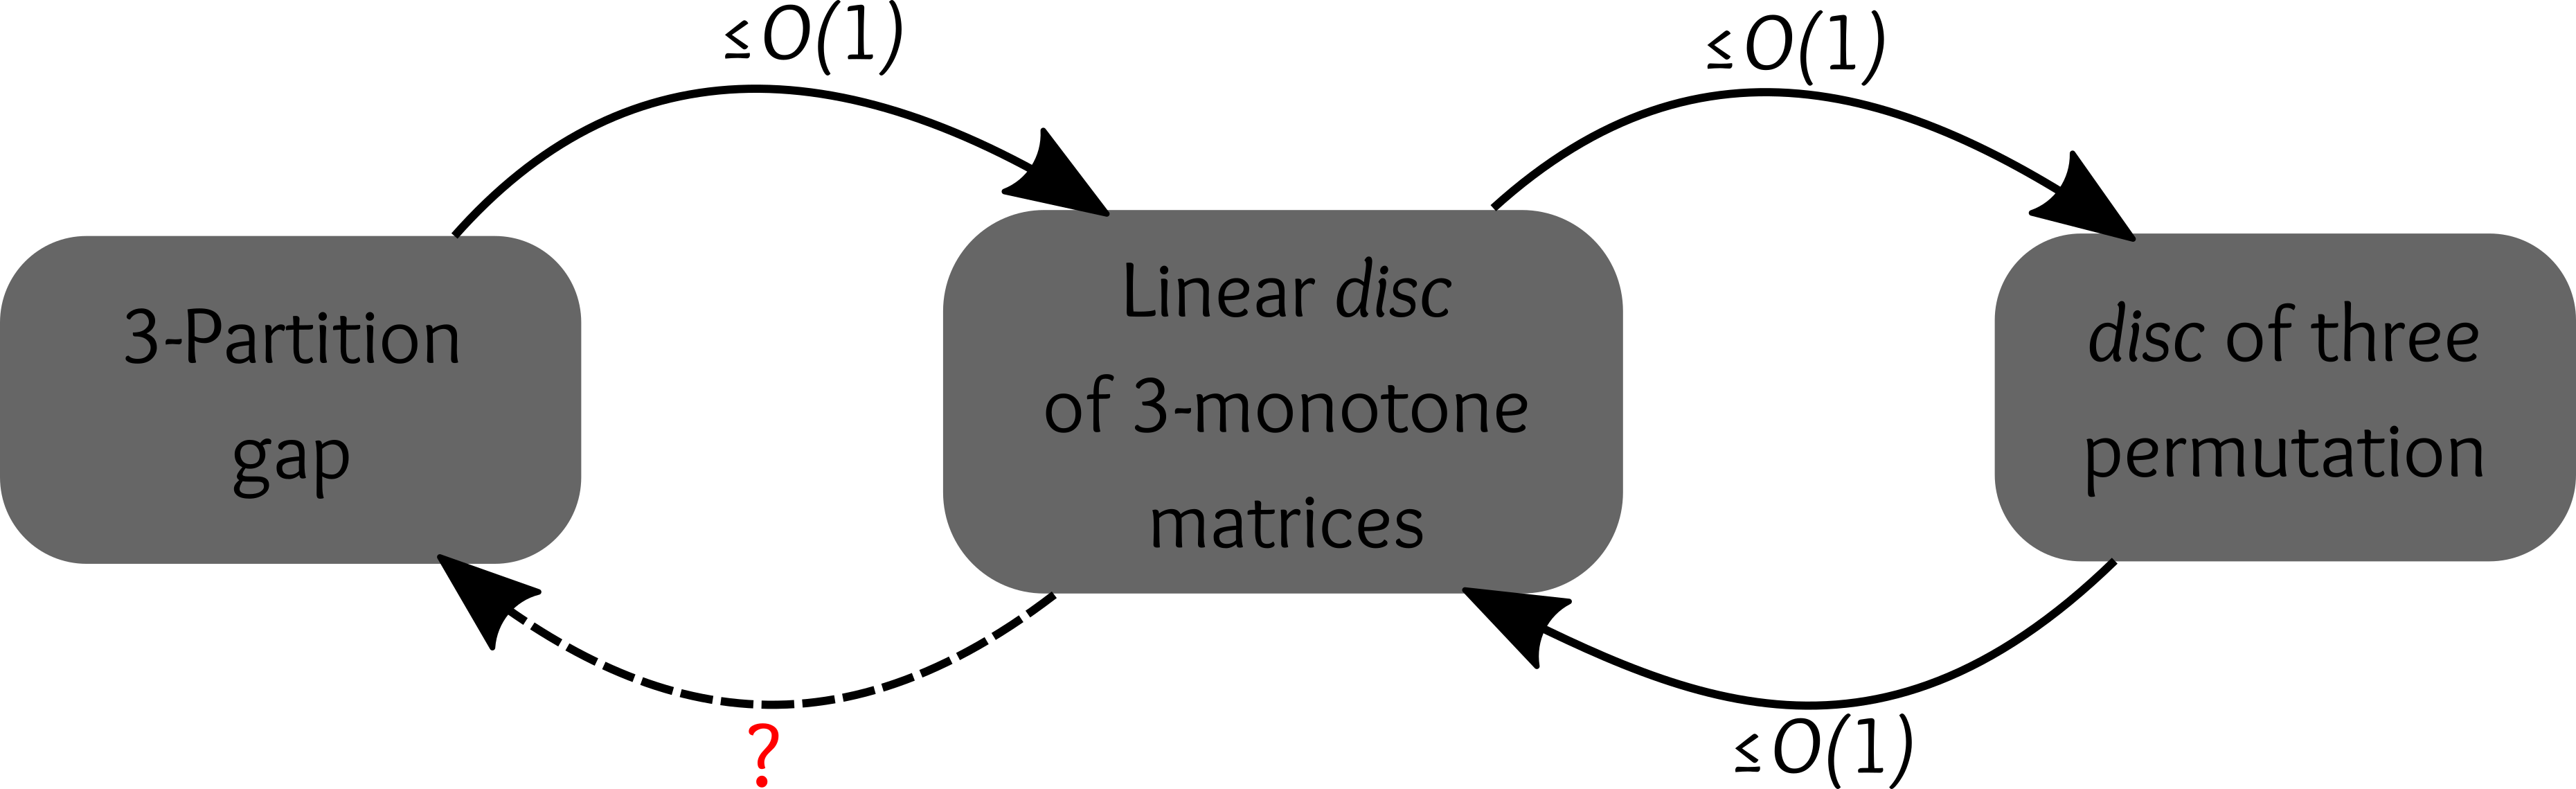
\includegraphics[scale=0.6]{figure/soda_11_3perm.png}
%     \end{figure}
    
%     \begin{itemize}
%         \item  $\mathsf{A}$ is \b{3-monotone} if 
%         \begin{itemize}
%             \item  entries $a_{ij} \in \mathsf{A}$ belong to $\{0,\ldots,3\}$
%             \item  columns are monotone increasing
%         \end{itemize}
%     \end{itemize}
% \end{frame}

\begin{frame}{Why Discrepancy Theory Inspired 3-Partition Instances?}
    \begin{itemize}
        \item<1->  For \b{3-Partition case}, all three,~\cite{karmarkar1982efficient, rothvoss2013approximating, hoberg2017logarithmic} give an upper bound of $\a{O(\log n)}$ on integrality gap.
    \end{itemize}
    
    \onslide<2->{\begin{alertblock}{~\cite{newman2012beck} (Disprove Beck's conjecture)}
        Let $\mathcal{S}_k$ be the family of prefixes of three permutations $\pi_1, \pi_2, \pi_3$ on $m = 3^k$ elements. Then, $disc(\mathcal{S}_k)$ is $\Omega(\log m)$.
    \end{alertblock}}
    
    \onslide<3->{\begin{alertblock}{~\cite{newman2012beck} (Consequence to bin packing)}
        There exists a bin packing instance $I = (n,s)$ with an optimal basic feasible solution $x$ to GGLP, such that any integral solution $y$ to GGLP satisfying $\text{supp}(y) \subseteq \text{supp}(x)$ has value at least $\mathsf{OPT}(I)+\Omega(\log n)$.
    \end{alertblock}}
\end{frame}


% \begin{frame}{Badly Three Colorable Permutations: Construction}

% Given $\pi^{k}_1, \pi_2^{k}, \pi_3^{k}$ on $m= 3^k$ elements for $k \in \mathbb{N}$, $\pi^{k+1}_1, \pi_2^{k+1}, \pi_3^{k+1}$ are obtained as follows:
% \begin{itemize}
%     \item  Partition $[3^{k+1}]$ into three intervals $A_k, B_k, C_k$ of equal size $3^k$, that is, let $A_k = [3^k]$, $B_k = [3^k + 1, 2\cdot3^k]$ and $C_k = [2\cdot3^k + 1, 3^{k+1}]$. 
    
%     \item  For $h \in [3]$, define $\pi_h^k$ as

%         \begin{equation*}
%         \begin{aligned}
%         & & & \pi_h^k(l + 3^k) = \pi_h^k(l) + 3^k &&&&& \forall l \in [3^k] \\
%         & & & \pi_h^k(l + 2 \cdot 3^k) = \pi_h^k(l) + 2 \cdot  3^k &&&&& \forall l \in [3^k]
%         \end{aligned}
%         \end{equation*}
        
%     \item  Finally, we obtain $\pi_h^{k+1} \ \forall h \in [3]$ 
%         \begin{equation*}
%         \begin{aligned}
%         \pi_1^{k+1} = \pi_1^k(A_k) \quad \pi_1^k(B_k) \quad \pi_1^k(C_k) \\
%         \pi_2^{k+1} = \pi_2^k(C_k) \quad \pi_2^k(A_k) \quad \pi_2^k(B_k) \\
%         \pi_3^{k+1} = \pi_3^k(B_k) \quad \pi_3^k(C_k) \quad \pi_3^k(A_k) \\
%         \end{aligned}
%         \end{equation*}


% \end{itemize}
    
% \end{frame}


\begin{frame}{Badly Three Colorable Permutations: Illustration}

\begin{columns}
    \onslide<1->{\begin{column}{0.47\textwidth}
        \begin{table}[]
        \centering
        \begin{tabular}{llll}
        $\pi_1$ & {\color[HTML]{FE0000} A} & {\color[HTML]{3531FF} B} & {\color[HTML]{32CB00} C} \\
        $\pi_2$ & {\color[HTML]{32CB00} C} & {\color[HTML]{FE0000} A} & {\color[HTML]{3531FF} B} \\
        $\pi_3$ & {\color[HTML]{3531FF} B} & {\color[HTML]{32CB00} C} & {\color[HTML]{FE0000} A}
        \end{tabular}
        \end{table}
    \end{column}}
    
    \onslide<2->{\begin{column}{0.5\textwidth}
        \begin{table}[]
        \begin{tabular}{llll}
        $\pi_1^{k=1}$ & {\color[HTML]{FE0000} 1} & {\color[HTML]{3531FF} 2} & {\color[HTML]{32CB00} 3} \\
        $\pi_2^{k=1}$ & {\color[HTML]{32CB00} 3} & {\color[HTML]{FE0000} 1} & {\color[HTML]{3531FF} 2} \\
        $\pi_3^{k=1}$ & {\color[HTML]{3531FF} 2} & {\color[HTML]{32CB00} 3} & {\color[HTML]{FE0000} 1}
        \end{tabular}
        \end{table}
    \end{column}}
\end{columns}



% \begin{minipage}{0.47\textwidth}
% \begin{table}[]
% \centering
% \begin{tabular}{llll}
% $\pi_1$ & {\color[HTML]{FE0000} A} & {\color[HTML]{3531FF} B} & {\color[HTML]{32CB00} C} \\
% $\pi_2$ & {\color[HTML]{32CB00} C} & {\color[HTML]{FE0000} A} & {\color[HTML]{3531FF} B} \\
% $\pi_3$ & {\color[HTML]{3531FF} B} & {\color[HTML]{32CB00} C} & {\color[HTML]{FE0000} A}
% \end{tabular}
% \end{table}
% \end{minipage}

% \begin{minipage}{0.5\textwidth}
%   \begin{table}[]
% \begin{tabular}{llll}
% $\pi^{k=1}_1$ & {\color[HTML]{FE0000} 1} & {\color[HTML]{3531FF} 2} & {\color[HTML]{32CB00} 3}
% \end{tabular}
% \end{table}
% \end{minipage}

\only<3>{\begin{table}[]
\begin{tabular}{llllllllll}
$\pi^{k=2}_1$ & 1 & 2 & 3 & 4 & 5 & 6 & 7 & 8 & 9
\end{tabular}
\end{table}}

\only<4>{\begin{table}[]
\begin{tabular}{llllllllll}
$\pi^{k=2}_1$ & {\color[HTML]{FE0000} 1} & {\color[HTML]{FE0000} 2} & {\color[HTML]{FE0000} 3} & {\color[HTML]{3531FF} 4} & {\color[HTML]{3531FF} 5} & {\color[HTML]{3531FF} 6} & {\color[HTML]{32CB00} 7} & {\color[HTML]{32CB00} 8} & {\color[HTML]{32CB00} 9}
\end{tabular}
\end{table}}

\only<5>{\begin{table}[]
\begin{tabular}{llllllllll}
$\pi_1^{k=2}$ & {\color[HTML]{FE0000} 1} & {\color[HTML]{FE0000} 2} & {\color[HTML]{FE0000} 3} & {\color[HTML]{3531FF} 4} & {\color[HTML]{3531FF} 5} & {\color[HTML]{3531FF} 6} & {\color[HTML]{32CB00} 7} & {\color[HTML]{32CB00} 8} & {\color[HTML]{32CB00} 9} \\
$\pi_2^{k=2}$ & {\color[HTML]{32CB00} 7} & {\color[HTML]{32CB00} 8} & {\color[HTML]{32CB00} 9} & {\color[HTML]{FE0000} 1} & {\color[HTML]{FE0000} 2} & {\color[HTML]{FE0000} 3} & {\color[HTML]{3166FF} 4} & {\color[HTML]{3166FF} 5} & {\color[HTML]{3166FF} 6} \\
$\pi_3^{k=2}$ & {\color[HTML]{3531FF} 4} & {\color[HTML]{3531FF} 5} & {\color[HTML]{3531FF} 6} & {\color[HTML]{32CB00} 7} & {\color[HTML]{32CB00} 8} & {\color[HTML]{32CB00} 9} & {\color[HTML]{FE0000} 1} & {\color[HTML]{FE0000} 2} & {\color[HTML]{FE0000} 3}
\end{tabular}
\end{table}}

% \only<6>{
% \begin{table}[]
% \begin{tabular}{llllllllll}
% $\pi_1^{k=1}$ & {\color[HTML]{FE0000} 1} & {\color[HTML]{3531FF} 2} & {\color[HTML]{32CB00} 3} & {\color[HTML]{FE0000} 4} & {\color[HTML]{3531FF} 5} & {\color[HTML]{32CB00} 6} & {\color[HTML]{FE0000} 7} & {\color[HTML]{3531FF} 8} & {\color[HTML]{32CB00} 9} \\
% $\pi_2^{k=1}$ & {\color[HTML]{FE0000} 7} & {\color[HTML]{3531FF} 8} & {\color[HTML]{32CB00} 9} & {\color[HTML]{FE0000} 1} & {\color[HTML]{3531FF} 2} & {\color[HTML]{32CB00} 3} & {\color[HTML]{FE0000} 4} & {\color[HTML]{3531FF} 5} & {\color[HTML]{32CB00} 6} \\
% $\pi_3^{k=1}$ & {\color[HTML]{FE0000} 4} & {\color[HTML]{3531FF} 5} & {\color[HTML]{32CB00} 6} & {\color[HTML]{FE0000} 7} & {\color[HTML]{3531FF} 8} & {\color[HTML]{32CB00} 9} & {\color[HTML]{FE0000} 1} & {\color[HTML]{3531FF} 2} & {\color[HTML]{32CB00} 3}
% \end{tabular}
% \end{table}
% }

\only<6>{
\begin{table}[]
\begin{tabular}{llllllllll}
$\pi_1^{k=2}$ & {\color[HTML]{FE0000} 1} & {\color[HTML]{3531FF} 2} & {\color[HTML]{32CB00} 3} & {\color[HTML]{FE0000} 4} & {\color[HTML]{3531FF} 5} & {\color[HTML]{32CB00} 6} & {\color[HTML]{FE0000} 7} & {\color[HTML]{3531FF} 8} & {\color[HTML]{32CB00} 9} \\
$\pi_2^{k=2}$ & {\color[HTML]{32CB00} 7} & {\color[HTML]{32CB00} 8} & {\color[HTML]{32CB00} 9} & {\color[HTML]{FE0000} 1} & {\color[HTML]{FE0000} 2} & {\color[HTML]{FE0000} 3} & {\color[HTML]{3166FF} 4} & {\color[HTML]{3166FF} 5} & {\color[HTML]{3166FF} 6} \\
$\pi_3^{k=2}$ & {\color[HTML]{3531FF} 4} & {\color[HTML]{3531FF} 5} & {\color[HTML]{3531FF} 6} & {\color[HTML]{32CB00} 7} & {\color[HTML]{32CB00} 8} & {\color[HTML]{32CB00} 9} & {\color[HTML]{FE0000} 1} & {\color[HTML]{FE0000} 2} & {\color[HTML]{FE0000} 3}
\end{tabular}
\end{table}}

\only<7>{
\begin{table}[]
\begin{tabular}{llllllllll}
$\pi^{k=2}_1$ & 1 & 2 & 3 & 4 & 5 & 6 & 7 & 8 & 9 \\
$\pi_2^{k=2}$ & {\color[HTML]{32CB00} 7} & {\color[HTML]{32CB00} 8} & {\color[HTML]{32CB00} 9} & {\color[HTML]{FE0000} 1} & {\color[HTML]{FE0000} 2} & {\color[HTML]{FE0000} 3} & {\color[HTML]{3166FF} 4} & {\color[HTML]{3166FF} 5} & {\color[HTML]{3166FF} 6} \\
$\pi_3^{k=2}$ & {\color[HTML]{3531FF} 4} & {\color[HTML]{3531FF} 5} & {\color[HTML]{3531FF} 6} & {\color[HTML]{32CB00} 7} & {\color[HTML]{32CB00} 8} & {\color[HTML]{32CB00} 9} & {\color[HTML]{FE0000} 1} & {\color[HTML]{FE0000} 2} & {\color[HTML]{FE0000} 3}
\end{tabular}
\end{table}}

\only<8>{
\begin{table}[]
\begin{tabular}{llllllllll}
$\pi^{k=2}_1$ & 1 & 2 & 3 & 4 & 5 & 6 & 7 & 8 & 9 \\
$\pi_2^{k=2}$ & {\color[HTML]{FE0000} 7} & {\color[HTML]{3531FF} 8} & {\color[HTML]{32CB00} 9} & {\color[HTML]{FE0000} 1} & {\color[HTML]{3531FF} 2} & {\color[HTML]{32CB00} 3} & {\color[HTML]{FE0000} 4} & {\color[HTML]{3531FF} 5} & {\color[HTML]{32CB00} 6} \\
$\pi_3^{k=2}$ & {\color[HTML]{3531FF} 4} & {\color[HTML]{3531FF} 5} & {\color[HTML]{3531FF} 6} & {\color[HTML]{32CB00} 7} & {\color[HTML]{32CB00} 8} & {\color[HTML]{32CB00} 9} & {\color[HTML]{FE0000} 1} & {\color[HTML]{FE0000} 2} & {\color[HTML]{FE0000} 3}
\end{tabular}
\end{table}}


\only<9>{
\begin{table}[]
\begin{tabular}{llllllllll}
$\pi^{k=2}_1$ & 1 & 2 & 3 & 4 & 5 & 6 & 7 & 8 & 9 \\
$\pi_2^{k=2}$ & {\color[HTML]{32CB00} 9} & {\color[HTML]{FE0000} 7} & {\color[HTML]{3531FF} 8} & {\color[HTML]{32CB00} 3} & {\color[HTML]{FE0000} 1} & {\color[HTML]{3531FF} 2} & {\color[HTML]{32CB00} 6} & {\color[HTML]{FE0000} 4} & {\color[HTML]{3531FF} 5} \\
$\pi_3^{k=2}$ & {\color[HTML]{3531FF} 4} & {\color[HTML]{3531FF} 5} & {\color[HTML]{3531FF} 6} & {\color[HTML]{32CB00} 7} & {\color[HTML]{32CB00} 8} & {\color[HTML]{32CB00} 9} & {\color[HTML]{FE0000} 1} & {\color[HTML]{FE0000} 2} & {\color[HTML]{FE0000} 3}
\end{tabular}
\end{table}}


\only<10>{
\begin{table}[]
\begin{tabular}{llllllllll}
$\pi^{k=2}_1$ & 1 & 2 & 3 & 4 & 5 & 6 & 7 & 8 & 9 \\
$\pi_2^{k=2}$ & 9 & 7 & 8 & 3 & 1 & 2 & 6 & 4 & 5 \\
$\pi_3^{k=2}$ & {\color[HTML]{3531FF} 4} & {\color[HTML]{3531FF} 5} & {\color[HTML]{3531FF} 6} & {\color[HTML]{32CB00} 7} & {\color[HTML]{32CB00} 8} & {\color[HTML]{32CB00} 9} & {\color[HTML]{FE0000} 1} & {\color[HTML]{FE0000} 2} & {\color[HTML]{FE0000} 3}
\end{tabular}
\end{table}}


\only<11>{
\begin{table}[]
\begin{tabular}{llllllllll}
$\pi^{k=2}_1$ & 1 & 2 & 3 & 4 & 5 & 6 & 7 & 8 & 9 \\
$\pi_2^{k=2}$ & 9 & 7 & 8 & 3 & 1 & 2 & 6 & 4 & 5 \\
$\pi_3^{k=2}$ & 5 & 6 & 4 & 8 & 9 & 7 & 2 & 3 & 1
\end{tabular}
\end{table}}


% \begin{figure}
% \centering
% \begin{tabular}{
% >{\columncolor[HTML]{FFFFFF}}l 
% >{\columncolor[HTML]{FFFFFF}}l 
% >{\columncolor[HTML]{FFFFFF}}l 
% >{\columncolor[HTML]{FFFFFF}}l 
% >{\columncolor[HTML]{FFFFFF}}l 
% >{\columncolor[HTML]{FFFFFF}}l 
% >{\columncolor[HTML]{FFFFFF}}l 
% >{\columncolor[HTML]{FFFFFF}}l 
% >{\columncolor[HTML]{FFFFFF}}l }
% {\color[HTML]{CB0000} 1} & {\color[HTML]{CB0000} 2} & {\color[HTML]{CB0000} 3} & {\color[HTML]{009901} 4} & {\color[HTML]{009901} 5} & {\color[HTML]{009901} 6} & {\color[HTML]{00009B} 7} & {\color[HTML]{00009B} 8} & {\color[HTML]{00009B} 9} \\
% {\color[HTML]{303498} 9} & {\color[HTML]{303498} 7} & {\color[HTML]{303498} 8} & {\color[HTML]{CB0000} 3} & {\color[HTML]{CB0000} 1} & {\color[HTML]{CB0000} 2} & {\color[HTML]{009901} 6} & {\color[HTML]{009901} 4} & {\color[HTML]{009901} 5} \\
% {\color[HTML]{009901} 5} & {\color[HTML]{009901} 6} & {\color[HTML]{009901} 4} & {\color[HTML]{00009B} 8} & {\color[HTML]{00009B} 9} & {\color[HTML]{00009B} 7} & {\color[HTML]{CB0000} 2} & {\color[HTML]{CB0000} 3} & {\color[HTML]{CB0000} 1}
% \end{tabular}
% \caption{Three permutations for $m = 9 \; (k=2)$}
% \end{figure}


% \begin{figure}
% \tiny
% \hskip-2.7cm
% \begin{tabular}{
% >{\columncolor[HTML]{FFFFFF}}l 
% >{\columncolor[HTML]{FFFFFF}}l 
% >{\columncolor[HTML]{FFFFFF}}l 
% >{\columncolor[HTML]{FFFFFF}}l 
% >{\columncolor[HTML]{FFFFFF}}l 
% >{\columncolor[HTML]{FFFFFF}}l 
% >{\columncolor[HTML]{FFFFFF}}l 
% >{\columncolor[HTML]{FFFFFF}}l 
% >{\columncolor[HTML]{FFFFFF}}l 
% >{\columncolor[HTML]{FFFFFF}}l 
% >{\columncolor[HTML]{FFFFFF}}l 
% >{\columncolor[HTML]{FFFFFF}}l 
% >{\columncolor[HTML]{FFFFFF}}l 
% >{\columncolor[HTML]{FFFFFF}}l 
% >{\columncolor[HTML]{FFFFFF}}l 
% >{\columncolor[HTML]{FFFFFF}}l 
% >{\columncolor[HTML]{FFFFFF}}l 
% >{\columncolor[HTML]{FFFFFF}}l 
% >{\columncolor[HTML]{FFFFFF}}l 
% >{\columncolor[HTML]{FFFFFF}}l 
% >{\columncolor[HTML]{FFFFFF}}l 
% >{\columncolor[HTML]{FFFFFF}}l 
% >{\columncolor[HTML]{FFFFFF}}l 
% >{\columncolor[HTML]{FFFFFF}}l 
% >{\columncolor[HTML]{FFFFFF}}l 
% >{\columncolor[HTML]{FFFFFF}}l 
% >{\columncolor[HTML]{FFFFFF}}l }
% {\color[HTML]{CB0000} 1}  & {\color[HTML]{CB0000} 2}  & {\color[HTML]{CB0000} 3}  & {\color[HTML]{CB0000} 4}  & {\color[HTML]{CB0000} 5}  & {\color[HTML]{CB0000} 6}  & {\color[HTML]{CB0000} 7}  & {\color[HTML]{CB0000} 8}  & {\color[HTML]{CB0000} 9}  & {\color[HTML]{009901} 10} & {\color[HTML]{009901} 11} & {\color[HTML]{009901} 12} & {\color[HTML]{009901} 13} & {\color[HTML]{009901} 14} & {\color[HTML]{009901} 15} & {\color[HTML]{009901} 16} & {\color[HTML]{009901} 17} & {\color[HTML]{009901} 18} & {\color[HTML]{00009B} 19} & {\color[HTML]{00009B} 20} & {\color[HTML]{00009B} 21} & {\color[HTML]{00009B} 22} & {\color[HTML]{00009B} 23} & {\color[HTML]{00009B} 24} & {\color[HTML]{00009B} 25} & {\color[HTML]{00009B} 26} & {\color[HTML]{00009B} 27} \\
% {\color[HTML]{303498} 27} & {\color[HTML]{303498} 25} & {\color[HTML]{303498} 26} & {\color[HTML]{303498} 21} & {\color[HTML]{303498} 19} & {\color[HTML]{303498} 20} & {\color[HTML]{303498} 24} & {\color[HTML]{303498} 22} & {\color[HTML]{303498} 23} & {\color[HTML]{CB0000} 9}  & {\color[HTML]{CB0000} 7}  & {\color[HTML]{CB0000} 8}  & {\color[HTML]{CB0000} 3}  & {\color[HTML]{CB0000} 1}  & {\color[HTML]{CB0000} 2}  & {\color[HTML]{CB0000} 6}  & {\color[HTML]{CB0000} 4}  & {\color[HTML]{CB0000} 5}  & {\color[HTML]{009901} 18} & {\color[HTML]{009901} 16} & {\color[HTML]{009901} 17} & {\color[HTML]{009901} 12} & {\color[HTML]{009901} 10} & {\color[HTML]{009901} 11} & {\color[HTML]{009901} 15} & {\color[HTML]{009901} 13} & {\color[HTML]{009901} 14} \\
% {\color[HTML]{009901} 14} & {\color[HTML]{009901} 15} & {\color[HTML]{009901} 13} & {\color[HTML]{009901} 17} & {\color[HTML]{009901} 18} & {\color[HTML]{009901} 16} & {\color[HTML]{009901} 11} & {\color[HTML]{009901} 12} & {\color[HTML]{009901} 10} & {\color[HTML]{00009B} 23} & {\color[HTML]{00009B} 24} & {\color[HTML]{00009B} 22} & {\color[HTML]{00009B} 26} & {\color[HTML]{00009B} 27} & {\color[HTML]{00009B} 25} & {\color[HTML]{00009B} 20} & {\color[HTML]{00009B} 21} & {\color[HTML]{00009B} 19} & {\color[HTML]{CB0000} 5}                         & {\color[HTML]{CB0000} 6}  & {\color[HTML]{CB0000} 4}  & {\color[HTML]{CB0000} 8}  & {\color[HTML]{CB0000} 9}  & {\color[HTML]{CB0000} 7}  & {\color[HTML]{CB0000} 2}  & {\color[HTML]{CB0000} 3}  & {\color[HTML]{CB0000} 1} 
% \end{tabular}
% \caption{Three permutations for $m = 27 \ (k=3)$}
% \end{figure}
    
\end{frame}


\begin{frame}{BP Instance from Badly Colorable Three Permutations: Construction}
    
\begin{minipage}
\linewidth
\tiny
\begin{equation*}\label{fig:33}
\begin{aligned}
\pi_1^{k=2} \qquad \quad \underline{1 \quad 2} \quad \underline{\mathbf{3 \quad 4}} \quad \underline{5 \quad 6} \quad \underline{7 \quad 8} \quad \underline{9 \quad 0} \\
\pi_2^{k=2} \qquad  \quad \underline{9 \quad 7} \quad \underline{8 \quad 3} \quad \underline{1 \quad 2} \quad \underline{\mathbf{6 \quad 4}} \quad \underline{5 \quad 0} \\
\pi_3^{k=2} \qquad \quad \underline{5 \quad 6} \quad \underline{\mathbf{4 \quad 8}} \quad \underline{9 \quad 7} \quad \underline{2 \quad 3} \quad \underline{1 \quad 0}
\end{aligned}
\end{equation*}
% {\captionof{figure}{Construction of bin packing instance for $k=2$, each underlined pair is an item. The pairs in bold correspond to the packing of pattern $p_4$.}}
\end{minipage}


\begin{figure}[!ht]\label{fig:34}
\centering
\tiny
\begin{tabular}{l|llllllllll}
& $p_1$ & $p_2$ & $p_3$ & \textbf{$p_4$} & $p_5$ & $p_6$ & $p_7$ & $p_8$ & $p_9$ & $p_0$ \\ \hline
$s_1$ & 1 & 1 & 0 & \textbf{0} & 0 & 0 & 0 & 0 & 0 & 0 \\
$s_2$ & 0 & 0 & 1 & \textbf{1} & 0 & 0 & 0 & 0 & 0 & 0 \\
$s_3$ & 0 & 0 & 0 & \textbf{0} & 1 & 1 & 0 & 0 & 0 & 0 \\
$s_4$ & 0 & 0 & 0 & \textbf{0} & 0 & 0 & 1 & 1 & 0 & 0 \\
$s_5$ & 0 & 0 & 0 & \textbf{0} & 0 & 0 & 0 & 0 & 1 & 1 \\ \hline
$s_6$ & 0 & 0 & 0 & \textbf{0} & 0 & 0 & 1 & 0 & 1 & 0 \\
$s_7$ & 0 & 0 & 1 & \textbf{0} & 0 & 0 & 0 & 1 & 0 & 0 \\
$s_8$ & 1 & 1 & 0 & \textbf{0} & 0 & 0 & 0 & 0 & 0 & 0 \\
$s_9$ & 0 & 0 & 0 & \textbf{1} & 0 & 1 & 0 & 0 & 0 & 0 \\
$s_{10}$ & 0 & 0 & 0 & \textbf{0} & 1 & 0 & 0 & 0 & 0 & 1 \\ \hline
$s_{11}$ & 0 & 0 & 0 & \textbf{0} & 1 & 1 & 0 & 0 & 0 & 0 \\
$s_{12}$ & 0 & 0 & 0 & \textbf{1} & 0 & 0 & 0 & 1 & 0 & 0 \\
$s_{13}$ & 0 & 0 & 0 & \textbf{0} & 0 & 0 & 1 & 0 & 1 & 0 \\
$s_{14}$ & 0 & 1 & 1 & \textbf{0} & 0 & 0 & 0 & 0 & 0 & 0 \\
$s_{15}$ & 1 & 0 & 0 & \textbf{0} & 0 & 0 & 0 & 0 & 0 & 1
\end{tabular}
% \caption{The constraint matrix $\mathsf{A}$ for the case $k=2$. The rows correspond to the items, in each block of $\frac{m+1}{2} = 5 $ are the items defined by one of the permutations. The $m+1 = 10$ correspond to the patterns. Recall that the last pattern is $p_0$.}
\end{figure}

% \begin{table}[]
% \centering
% \tiny
% \begin{tabular}{c|cccccccccc}
%          & $p_1$                     & $p_2$                     & $p_3$                     & {\color[HTML]{000000} \textbf{$p_4$}}                     & $p_5$                     & $p_6$                     & $p_7$                     & $p_8$                     & $p_9$                     & $p_0$                     \\ \hline
% $s_1$    & \cellcolor[HTML]{FFFFFF}1 & \cellcolor[HTML]{FFFFFF}1 & \cellcolor[HTML]{FFFFFF}0 & \cellcolor[HTML]{FFFFFF}{\color[HTML]{000000} \textbf{0}} & \cellcolor[HTML]{FFFFFF}0 & \cellcolor[HTML]{FFFFFF}0 & \cellcolor[HTML]{FFFFFF}0 & \cellcolor[HTML]{FFFFFF}0 & \cellcolor[HTML]{FFFFFF}0 & \cellcolor[HTML]{FFFFFF}0 \\
% $s_2$    & \cellcolor[HTML]{FFFFFF}0 & \cellcolor[HTML]{FFFFFF}0 & \cellcolor[HTML]{FFFFFF}1 & \cellcolor[HTML]{FFFFFF}{\color[HTML]{000000} \textbf{1}} & \cellcolor[HTML]{FFFFFF}0 & \cellcolor[HTML]{FFFFFF}0 & \cellcolor[HTML]{FFFFFF}0 & \cellcolor[HTML]{FFFFFF}0 & \cellcolor[HTML]{FFFFFF}0 & \cellcolor[HTML]{FFFFFF}0 \\
% $s_3$    & \cellcolor[HTML]{FFFFFF}0 & \cellcolor[HTML]{FFFFFF}0 & \cellcolor[HTML]{FFFFFF}0 & \cellcolor[HTML]{FFFFFF}{\color[HTML]{000000} \textbf{0}} & \cellcolor[HTML]{FFFFFF}1 & \cellcolor[HTML]{FFFFFF}1 & \cellcolor[HTML]{FFFFFF}0 & \cellcolor[HTML]{FFFFFF}0 & \cellcolor[HTML]{FFFFFF}0 & \cellcolor[HTML]{FFFFFF}0 \\
% $s_4$    & \cellcolor[HTML]{FFFFFF}0 & \cellcolor[HTML]{FFFFFF}0 & \cellcolor[HTML]{FFFFFF}0 & \cellcolor[HTML]{FFFFFF}{\color[HTML]{000000} \textbf{0}} & \cellcolor[HTML]{FFFFFF}0 & \cellcolor[HTML]{FFFFFF}0 & \cellcolor[HTML]{FFFFFF}1 & \cellcolor[HTML]{FFFFFF}1 & \cellcolor[HTML]{FFFFFF}0 & \cellcolor[HTML]{FFFFFF}0 \\
% $s_5$    & \cellcolor[HTML]{FFFFFF}0 & \cellcolor[HTML]{FFFFFF}0 & \cellcolor[HTML]{FFFFFF}0 & \cellcolor[HTML]{FFFFFF}{\color[HTML]{000000} \textbf{0}} & \cellcolor[HTML]{FFFFFF}0 & \cellcolor[HTML]{FFFFFF}0 & \cellcolor[HTML]{FFFFFF}0 & \cellcolor[HTML]{FFFFFF}0 & \cellcolor[HTML]{FFFFFF}1 & \cellcolor[HTML]{FFFFFF}1 \\ \hline
% $s_6$    & \cellcolor[HTML]{FFFFFF}0 & \cellcolor[HTML]{FFFFFF}0 & \cellcolor[HTML]{FFFFFF}0 & \cellcolor[HTML]{FFFFFF}{\color[HTML]{000000} \textbf{0}} & \cellcolor[HTML]{FFFFFF}0 & \cellcolor[HTML]{FFFFFF}0 & \cellcolor[HTML]{FFFFFF}1 & \cellcolor[HTML]{FFFFFF}0 & \cellcolor[HTML]{FFFFFF}1 & \cellcolor[HTML]{FFFFFF}0 \\
% $s_7$    & \cellcolor[HTML]{FFFFFF}0 & \cellcolor[HTML]{FFFFFF}0 & \cellcolor[HTML]{FFFFFF}1 & \cellcolor[HTML]{FFFFFF}{\color[HTML]{000000} \textbf{0}} & \cellcolor[HTML]{FFFFFF}0 & \cellcolor[HTML]{FFFFFF}0 & \cellcolor[HTML]{FFFFFF}0 & \cellcolor[HTML]{FFFFFF}1 & \cellcolor[HTML]{FFFFFF}0 & \cellcolor[HTML]{FFFFFF}0 \\
% $s_8$    & \cellcolor[HTML]{FFFFFF}1 & \cellcolor[HTML]{FFFFFF}1 & \cellcolor[HTML]{FFFFFF}0 & \cellcolor[HTML]{FFFFFF}{\color[HTML]{000000} \textbf{0}} & \cellcolor[HTML]{FFFFFF}0 & \cellcolor[HTML]{FFFFFF}0 & \cellcolor[HTML]{FFFFFF}0 & \cellcolor[HTML]{FFFFFF}0 & \cellcolor[HTML]{FFFFFF}0 & \cellcolor[HTML]{FFFFFF}0 \\
% $s_9$    & \cellcolor[HTML]{FFFFFF}0 & \cellcolor[HTML]{FFFFFF}0 & \cellcolor[HTML]{FFFFFF}0 & \cellcolor[HTML]{FFFFFF}{\color[HTML]{000000} \textbf{1}} & \cellcolor[HTML]{FFFFFF}0 & \cellcolor[HTML]{FFFFFF}1 & \cellcolor[HTML]{FFFFFF}0 & \cellcolor[HTML]{FFFFFF}0 & \cellcolor[HTML]{FFFFFF}0 & \cellcolor[HTML]{FFFFFF}0 \\
% $s_{10}$ & \cellcolor[HTML]{FFFFFF}0 & \cellcolor[HTML]{FFFFFF}0 & \cellcolor[HTML]{FFFFFF}0 & \cellcolor[HTML]{FFFFFF}{\color[HTML]{000000} \textbf{0}} & \cellcolor[HTML]{FFFFFF}1 & \cellcolor[HTML]{FFFFFF}0 & \cellcolor[HTML]{FFFFFF}0 & \cellcolor[HTML]{FFFFFF}0 & \cellcolor[HTML]{FFFFFF}0 & \cellcolor[HTML]{FFFFFF}1 \\ \hline
% $s_{11}$ & \cellcolor[HTML]{FFFFFF}0 & \cellcolor[HTML]{FFFFFF}0 & \cellcolor[HTML]{FFFFFF}0 & \cellcolor[HTML]{FFFFFF}{\color[HTML]{000000} \textbf{0}} & \cellcolor[HTML]{FFFFFF}1 & \cellcolor[HTML]{FFFFFF}1 & \cellcolor[HTML]{FFFFFF}0 & \cellcolor[HTML]{FFFFFF}0 & \cellcolor[HTML]{FFFFFF}0 & \cellcolor[HTML]{FFFFFF}0 \\
% $s_{12}$ & \cellcolor[HTML]{FFFFFF}0 & \cellcolor[HTML]{FFFFFF}0 & \cellcolor[HTML]{FFFFFF}0 & \cellcolor[HTML]{FFFFFF}{\color[HTML]{000000} \textbf{1}} & \cellcolor[HTML]{FFFFFF}0 & \cellcolor[HTML]{FFFFFF}0 & \cellcolor[HTML]{FFFFFF}0 & \cellcolor[HTML]{FFFFFF}1 & \cellcolor[HTML]{FFFFFF}0 & \cellcolor[HTML]{FFFFFF}0 \\
% $s_{13}$ & \cellcolor[HTML]{FFFFFF}0 & \cellcolor[HTML]{FFFFFF}0 & \cellcolor[HTML]{FFFFFF}0 & \cellcolor[HTML]{FFFFFF}{\color[HTML]{000000} \textbf{0}} & \cellcolor[HTML]{FFFFFF}0 & \cellcolor[HTML]{FFFFFF}0 & \cellcolor[HTML]{FFFFFF}1 & \cellcolor[HTML]{FFFFFF}0 & \cellcolor[HTML]{FFFFFF}1 & \cellcolor[HTML]{FFFFFF}0 \\
% $s_{14}$ & \cellcolor[HTML]{FFFFFF}0 & \cellcolor[HTML]{FFFFFF}1 & \cellcolor[HTML]{FFFFFF}1 & \cellcolor[HTML]{FFFFFF}{\color[HTML]{000000} \textbf{0}} & \cellcolor[HTML]{FFFFFF}0 & \cellcolor[HTML]{FFFFFF}0 & \cellcolor[HTML]{FFFFFF}0 & \cellcolor[HTML]{FFFFFF}0 & \cellcolor[HTML]{FFFFFF}0 & \cellcolor[HTML]{FFFFFF}0 \\
% $s_{15}$ & \cellcolor[HTML]{FFFFFF}1 & \cellcolor[HTML]{FFFFFF}0 & \cellcolor[HTML]{FFFFFF}0 & \cellcolor[HTML]{FFFFFF}{\color[HTML]{000000} \textbf{0}} & \cellcolor[HTML]{FFFFFF}0 & \cellcolor[HTML]{FFFFFF}0 & \cellcolor[HTML]{FFFFFF}0 & \cellcolor[HTML]{FFFFFF}0 & \cellcolor[HTML]{FFFFFF}0 & \cellcolor[HTML]{FFFFFF}1 \\ \hline
% \end{tabular}
% \end{table}



\end{frame}


\section{Implementation and Results}

% \begin{frame}{Generating Instances: Discrepancy Inspired 3-Partition Instances}

% \begin{itemize}
%     \item  Recall that, for 3-Partition instance $s_i \in (\frac{1}{4}, \frac{1}{2})$. Let $\mathcal{P}_k$ be the set of $3^k + 1$ patterns with $n = 3 \cdot \frac{3^k + 1}{2}$ items.
    
%         \item  SLP:
%         \begin{equation*}
%             \begin{aligned}
%                 & {\text{min}}
%                 & & 0 \\
%                 & \text{s.t.} & & \a{s^T p \leq 1} &&&& \forall p \in \mathcal{P}_k \\
%                 & & & s_i \leq \frac{1}{2} &&&& \forall i \in [n] \\
%                 & & & s_i \geq \frac{1}{4} &&&& \forall i \in [n]
%             \end{aligned}
%         \end{equation*}
    
% \end{itemize}
    
% \end{frame}

\begin{frame}{Generating Instances: Discrepancy Inspired 3-Partition Instances}

\begin{itemize}
    \onslide<1->{\item  Recall that, for 3-Partition instance $s_i \in (\frac{1}{4}, \frac{1}{2})$. Let $\mathcal{P}_k$ be the set of $3^k + 1$ patterns with $n = 3 \cdot \frac{3^k + 1}{2}$ items.}
        
    \onslide<2->{\item  SLP:
        \begin{equation*}
            \begin{aligned}
                & {\text{min}}
                & & 0 \\
                & \text{s.t.} & & \b{s^T p = 1} &&&& \forall p \in \mathcal{P}_k \\
                & & & s_i \leq \frac{1}{2} - \b{\frac{1}{8}} &&&& \forall i \in [n] \\
                & & & s_i \geq \frac{1}{4} + \b{\frac{1}{16}} &&&& \forall i \in [n]
            \end{aligned}
        \end{equation*}}
    
    % \onslide<3>{\item  \textbf{\b{Remark:}} Using Gurobi to solve SLP, the solutions have at least one third of all the items $s_i \in \{\frac{1}{4}, \frac{1}{2}\}$ since that has to be the case for a basic solution.}
    
\end{itemize}
    
\end{frame}


\begin{frame}{Generating Instances: Hindrance and its Remedy}
   
   \onslide<1->{\textbf{\b{Hindrance:}}}
    \begin{itemize}
        \item<1->  Infeasible SLP: 
            \begin{itemize}
                 \item<1-> Due to the constraint \b{$s^T p = 1$} as the size of the third item $s_o$ is determined by $s_o = 1 - s_l - s_m$ \a{(infeasible if $1- s_l - s_m < \frac{1}{4}$)}.
            
                \item<2-> Existence of patterns that share two items. 
            \end{itemize}
           
        % \item  Gurobi's bias towards upper bound $\frac{1}{2}$

    \end{itemize}
    
    \onslide<3->{\textbf{\b{Remedy:}}}
        \begin{itemize}
            \item<3-> Infeasible SLP:
                \begin{itemize}
                    % \item Try 1: 
                    %     \begin{itemize}
                    %         \item Incrementally traverse the patterns $p \in \mathcal{P}_k$ and assign size $s_i \in [\frac{1}{4}, \frac{1}{2}]$ to the randomly selected item and add to the SLP.
                            
                    %         \item If any item of the pattern is marked, then ignore and move to next one.
                    %     \end{itemize} 
                    % \item Try 2:
                    %     \begin{itemize}
                    %         \item Same procedure as Try 1 but the only difference is that, we also mark all items $s_l, s_m, s_o$ contained in the current pattern together with $s_{l+1}, s_{m+1}, s_{o+1}$ if they exist.
                    %     \end{itemize}
                    
                    \item<4-> Incrementally traverse each pattern and if any of the items is marked, then move to next one.
                    
                    \item<5-> If no item is marked, then choose an item randomly and assign a random number.
                    
                    \item<6-> Them mark all items $s_l, s_m, s_o$ contained in the current pattern together with $s_{l+1}, s_{m+1}, s_{o+1}$ if they exist.
                \end{itemize}
        \end{itemize}
    
%     \textbf{{\b{Remedies:}}
%     \begin{itemize}
%         \item  Traverse patterns incrementally and if item is marked, then goto next pattern.
        
%         \item  If no item is marked, then randomly select any item and assign it's size randomly.
        
%         \item  Lastly, also mark all items $s_l, s_m, s_o$ contained in the current pattern together with $s_{l+1}, s_{m+1}, s_{o+1}$ if they exist.
%     \end{itemize}
    
\end{frame}


\begin{frame}{Building LP: Hindrance and its Remedy}
    \onslide<1->{\textbf{\b{Hindrance:}} Generated GGLP explodes if one does not find patterns cleverly.}
    
    \onslide<2->{\textbf{\b{Remedy:}} Modify GGLP to GGLP* according to maximal patterns.}
    
    \begin{itemize}
        \item<2-> A $p \in \mathcal{P}$ is called \a{\emph{maximal}} if $0 \leq 1-s^T p < \min_{i \in [n]} s_i$.
        
        \item<3-> GGLP*:
        
            \begin{equation*}
                \begin{aligned}
                & {\text{min}}
                & & \sum_{p \in \mathcal{P}_{max}} x_p \\
                & \text{s.t.} & & \sum_{p \in \mathcal{P}_{max}} x_p p_i = b_i &&&& \forall i \in [n] \\
                & & & x_p \in \mathbb{R}_{\geq 0} &&&& \forall p \in \mathcal{P}_{max} 
                \end{aligned}
            \end{equation*}
        
        \item<4-> GGLP and GGLP* are \a{equivalent} formulations.
        
        % $\implies$ Can replace the non-maximal patterns in $\text{supp}(x)$ by convex combination of patterns $p \in \mathcal{P}_{max}$.
    \end{itemize}
\end{frame}

\begin{frame}{Results: Randomly generated Instances}
    \begin{itemize}
        \item<1-> Performed integrality tests for $70,000$ instances.
        
        \item<2-> \textbf{\b{Output:}} Only found $7$ non-IRUP instances $(1 < \text{gap} < 2)$\footnote{largest gap instance: $n=7$ and gap$=1.01786$}.
    \end{itemize}
    
    \onslide<3->{\begin{center}
            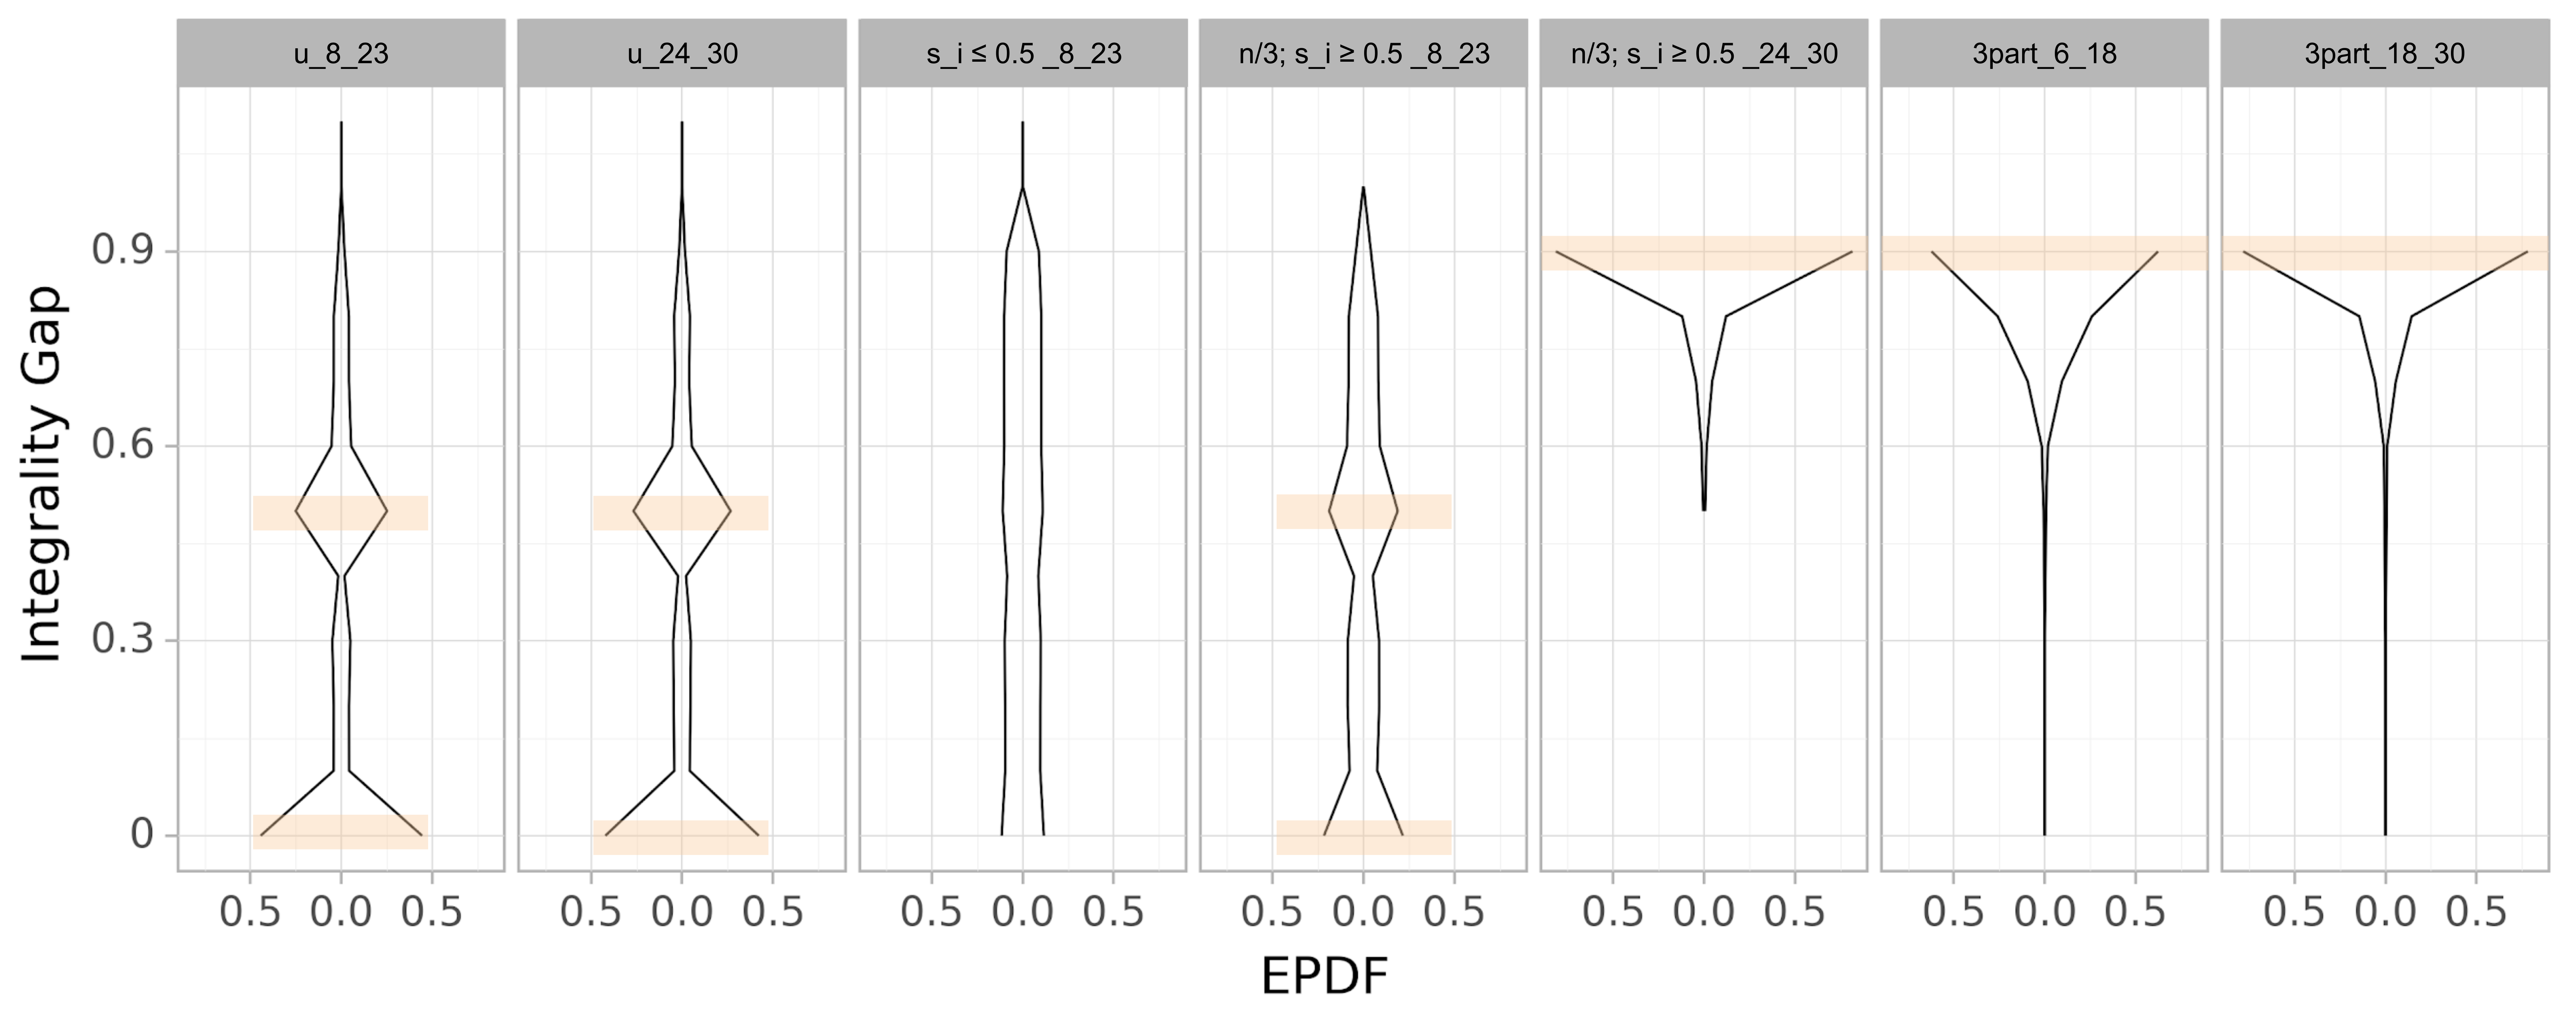
\includegraphics[scale=0.35]{figure/results-thesis.png}
    \end{center}}
\end{frame}


\begin{frame}{Results: Discrepancy Inspired 3-Partition Instances}
    \begin{itemize}
        \item<1-> Performed integrality tests for $24,750$ instances.
        
        \item<2-> \textbf{\b{Output:}} No non-IRUP instance found.
    \end{itemize}
    
% \onslide<3->{\begin{table}[]
% \centering
% \begin{tabular}{|c|l|c|c|c|}
% \hline
% \multirow{6}{*}{$\#$ Instances} & \multicolumn{4}{c|}{Integrality Gap}                                    \\ \cline{2-5} 
%                               &                          & 0    & {[}0.9,1) & 1                         \\ \cline{2-5} 
%                               & \multicolumn{1}{c|}{k=2} & 10000 & -         & -                         \\ \cline{2-5} 
%                               & k=3                      & 6202  & 986       & 2811                      \\ \cline{2-5} 
%                               & k=4                      & 0   & 1568       & \multicolumn{1}{l|}{3182} \\ \cline{2-5} 
%                               \hline
% \end{tabular}
%     % \caption{For $k=2,3$, 10000 instances were tested. While for $k=4$, 4750 instances were tested and we did not find any instance with gap$=0$ or gap$>1$.}
% \end{table}}

\onslide<3->{\begin{table}[]
\centering
\begin{tabular}{|c|l|c|c|c|}
\hline
\multirow{}{}{ Instances} & \multicolumn{4}{c|}{Integrality Gap}                                    \\ \cline{2-5} 
                              &                          & 0    & {[}0.9,1) & 1                         \\ \cline{2-5} 
                              & \multicolumn{1}{c|}{k=2} & 10000 & -         & -                         \\ \cline{2-5} 
                              & k=3                      & 6202  & 986       & 2811                      \\ \cline{2-5} 
                              & k=4                      & 0   & 1568       & \multicolumn{1}{l|}{3182} \\ \cline{2-5} 
                              \hline
\end{tabular}
    % \caption{For $k=2,3$, 10000 instances were tested. While for $k=4$, 4750 instances were tested and we did not find any instance with gap$=0$ or gap$>1$.}
\end{table}}

\end{frame}



\section{Problem II: Bin Packing for $O(1)$ different item types}

\begin{frame}{Bin Packing in Fixed Dimension: Polynomial Time Algorithms}

\textbf{\b{For constant $n$:}}

    \begin{itemize}

        \onslide<1->{\item  $\mathsf{OPT} + \mathbf{1}$ in time $2^{2^{O(n)}} \cdot (\log \Delta)^{O(1)}$~\cite{jansen2010opt}}
    
        \onslide<2->{\item  Exact Algorithm:\\
        In time $O(\log \Delta)^{2^{O(n)}}$~\cite{goemans2014polynomiality}}
        
        \onslide<3->{\item  An FPT Algorithm~\cite{jansen2016structure}: 
        \\
        In time $|V_I|^{2^{O(n)}} O(\log \Delta)^{O(1)}$ parameterized by $V_I$}  
    \end{itemize}
\end{frame}


\begin{frame}{Geometric View: From the Bird's Eye}
    \begin{itemize}
        \item Define $\mathsf{P} = \{x \in \mathbb{R}^n \mid s^{\text{T}} x \leq C\}$
    \end{itemize}
    
    \begin{center}
        \includegraphics<1>[scale=0.7]{figure/geometric_view_1.png}
        \includegraphics<2>[scale=0.7]{figure/geometric_view_2.png}
        \includegraphics<3>[scale=0.7]{figure/geometric_view_3.png}
        \includegraphics<4,5,6>[scale=0.7]{figure/geometric_view_4.png}
    \end{center}
    
    \only<5,6>{\textbf{\b{Hindrances:}}}
    \begin{itemize}
        \item<5-> Integral points in $\mathsf{P}$ are \a{exponentially} many.
        \item<6-> Weights can be \a{exponential} as well.
    \end{itemize}
    
\end{frame}



\begin{frame}{From decision variant to optimization variant}
    \onslide<1->{\textbf{\b{Bin Packing decision variant}}: Given an instance $I= (n,s,b,C,m)$, the decision variant consists in determining if there exists an assignment of items to $m$ bins of size $C$.}

    
    \begin{itemize}
        \item<2-> No objective function.
        
        \item <2->Can check if an instance $I$ has a solution with $k$ bins.
        
        \item<2-> Then use binary search to find the minimum $k$ for which $I$ is feasible 
        
        \item[]<3-> $\implies$  $\a{\mathsf{OPT}}$ \a{solution} for optimization variant.
    \end{itemize}
    
    \onslide<4->{\b{\textbf{Trivial UB:}}
        $UB = \max\{s^\text{T} x \mid x \in \{0, \ldots, b_1\} \times \ldots \times \{0, \ldots, b_n\}, s^\text{T} x \leq C \}$}
    
\end{frame}


% \begin{frame}{Preliminaries}

%     \onslide<1->{\b{\textbf{Dominating Pattern:}} $p_2$ dominates $p_1$, if $p_{1l} \leq p_{2l}, \ \forall l \in [n]$ and $\exists$ at least one $k \in [n]$ s.t. $p_{1k} < p_{2k}$.}
    
%     \begin{itemize}
%         \item<2->  \textbf{\b{Gilmore-Gomory LP Relaxation Revisited:}}
%             \begin{equation*}
%                 \begin{aligned}
%                      \bigg\{{\text{min}}
%                      \sum_{p \in \widetilde{\mathcal{P}}} \ x_p 
%                      \mid \sum_{p \in \widetilde{\mathcal{P}}} \ x_p \ p_i \ \a{\geq} \ b_i, \forall \ i \in [n];
%                     \ x_p \in \mathbb{R}_{\geq 0}, \forall \ p \in \widetilde{\mathcal{P}}\bigg\} 
%                 \end{aligned}
%             \end{equation*}
%     \end{itemize}
    
%     \onslide<3->{\b{\textbf{Trivial Upper Bound:}}\begin{equation*}
%         \begin{aligned}
%         UB = \max\{s^\text{T} x \mid x \in \{0, \ldots, b_1\} \times \ldots \times \{0, \ldots, b_n\}, s^\text{T} x \leq C \}
%         \end{aligned}
%     \end{equation*}}   
    
% \noindent    \begin{equation*}
%         \begin{aligned}
%         u_i = \min \Big\{b_i, \max_{k \in \mathbb{Z}_{\geq 0}} \{k \mid k \cdot s_i \leq C\} \Big\}, \forall i \in [n]
%         \end{aligned}
%     \end{equation*}

% \end{frame}



\begin{frame}{Feasibility Certificates}
    
    \begin{itemize}
        \item<1-> \b{\textbf{Bottleneck Instance:}} An instance $I = (n,s,b,C,m)$ is \emph{bottleneck} if $C$ adheres to the upper bound $UB$ 
        
        $\implies$ \a{Infeasibility Certificate!} (i.e. $m \cdot UB < s^{\text{T}} b$)  
    \end{itemize}
    
    \onslide<2->{\begin{alertblock}{Theorem~\cite{mccormick2001polynomial}}
        An instance $I = (n,s,b,C,m)$ is feasible \emph{iff}
        
        \begin{itemize}
            \item[1)]<2-> there exists $n+1$ many integral points in $\mathsf{P}$ s.t. the simplex $\mathsf{S}$ spanned by these points is unimodular, and
            
            \item[2)]<3-> the point $\overline{b} = \frac{b}{m} \in \mathsf{S}.$
        \end{itemize}
        
        \onslide<4->{As a partial converse, if $\overline{b} \notin \mathsf{P}$, then $I$ is infeasible.}
    \end{alertblock}}
    
\end{frame}


\begin{frame}{Bottleneck Instances and Feasibility}
    Consider an instance, \only<1,2>{$I = (3, (6,10,15)^\text{T}, (4,2,1)^\text{T}, \b{30}, 2)$} \onslide<3->{$I = (3, (6,10,15)^\text{T}, (4,2,1)^\text{T}, \a{28}, 2)$}
    
    \begin{center}
        \onslide<2->{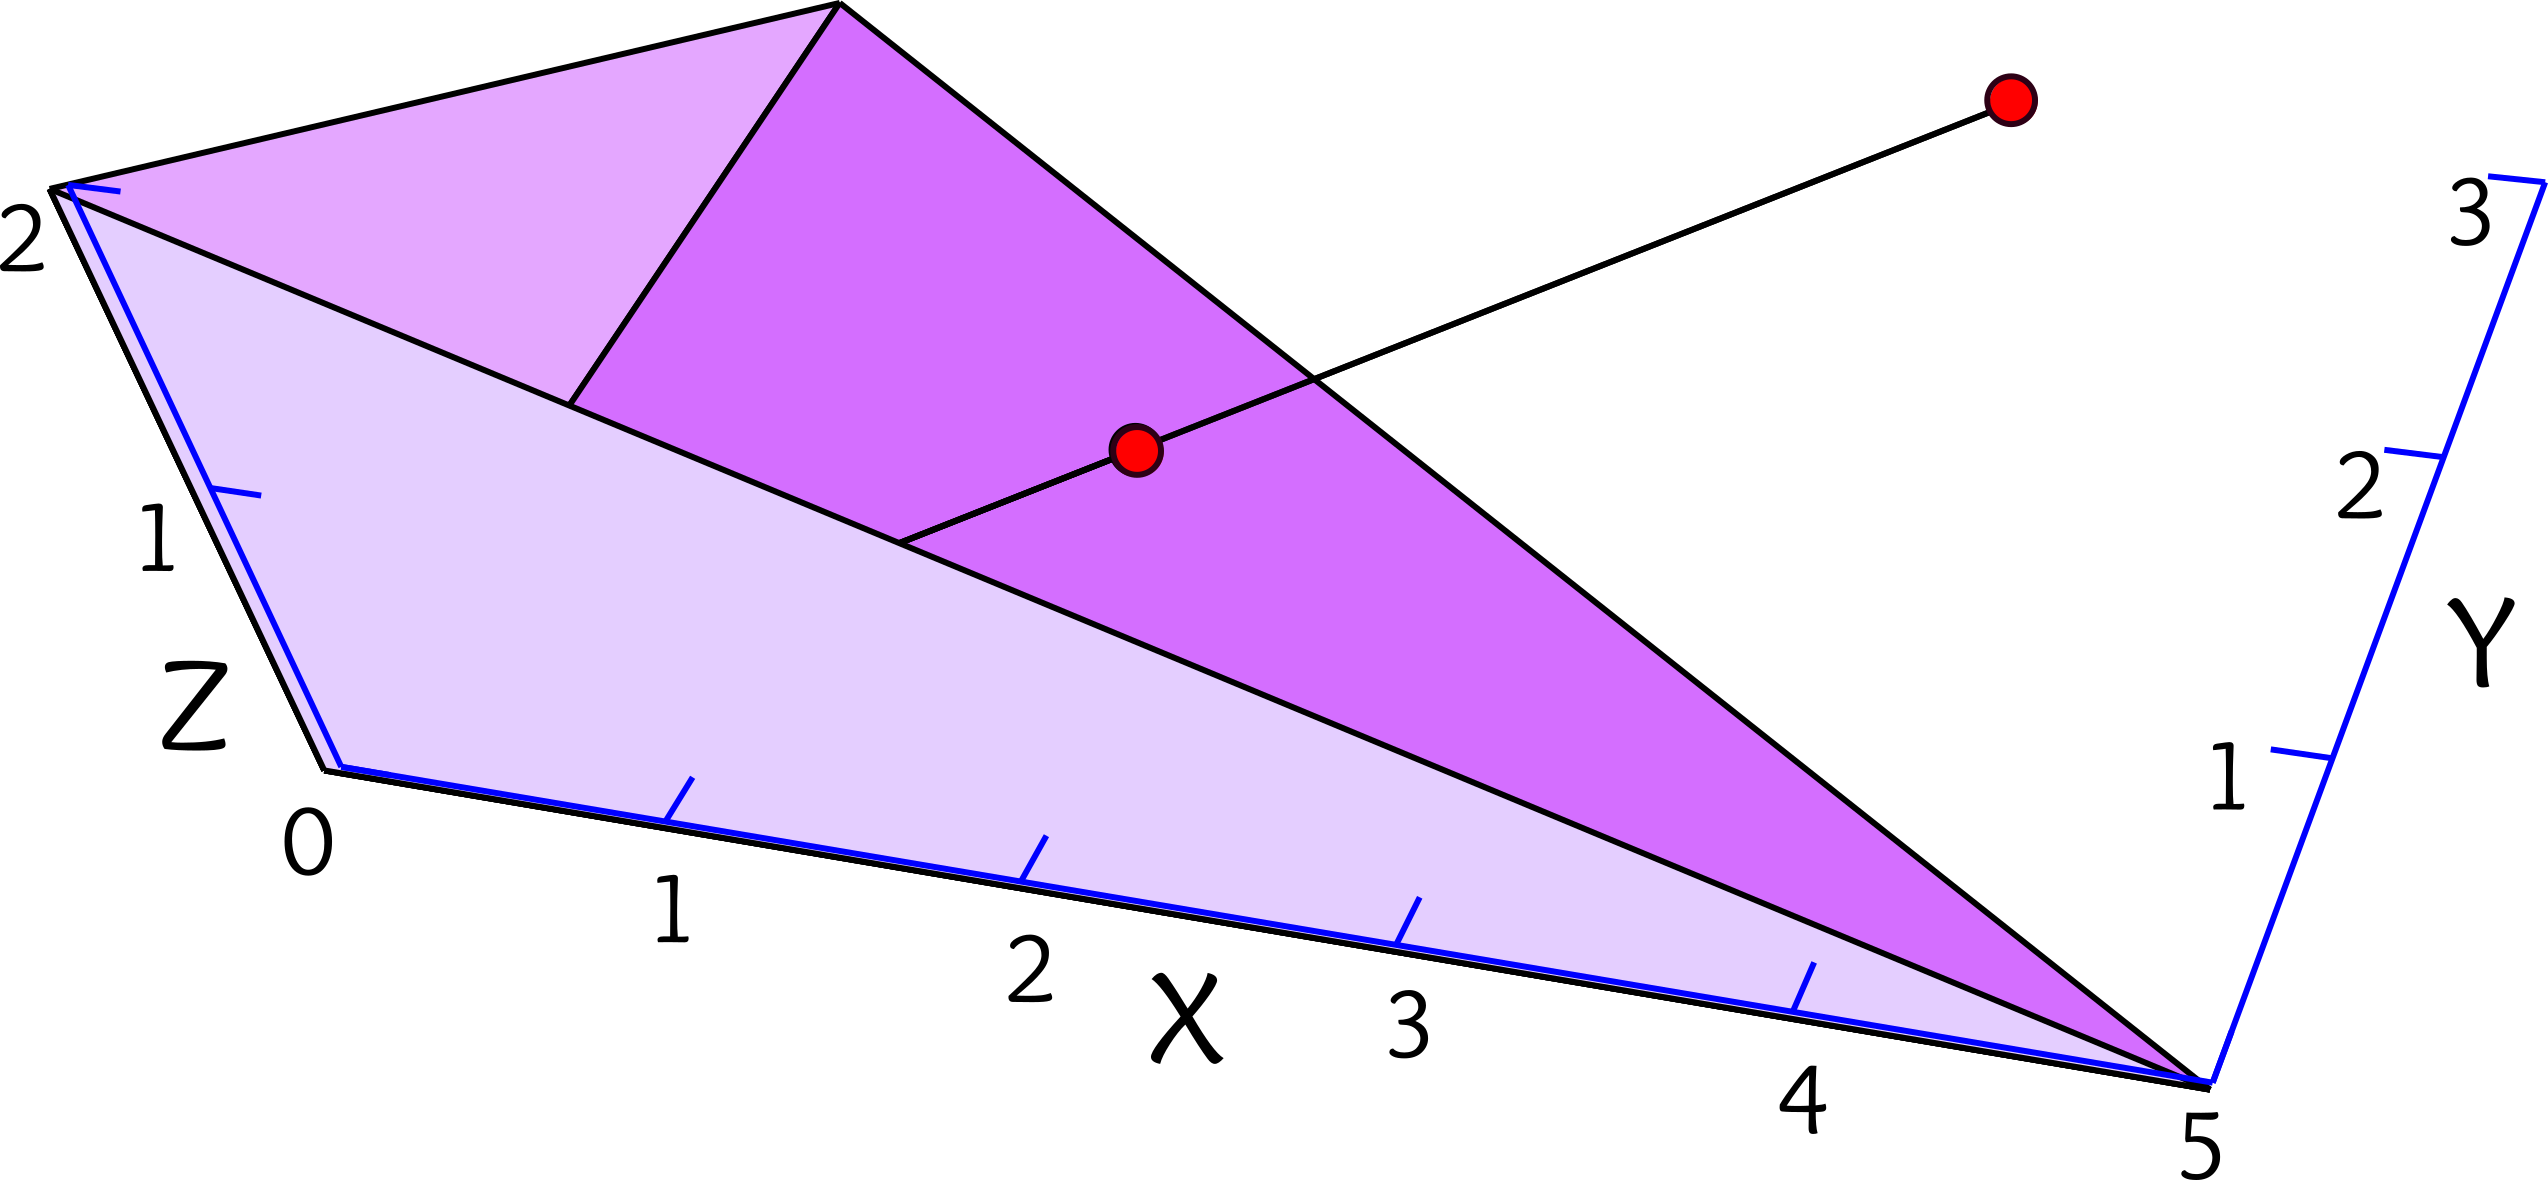
\includegraphics[scale=0.5]{figure/feasibility-bad1.png}}
        
        \onslide<3->{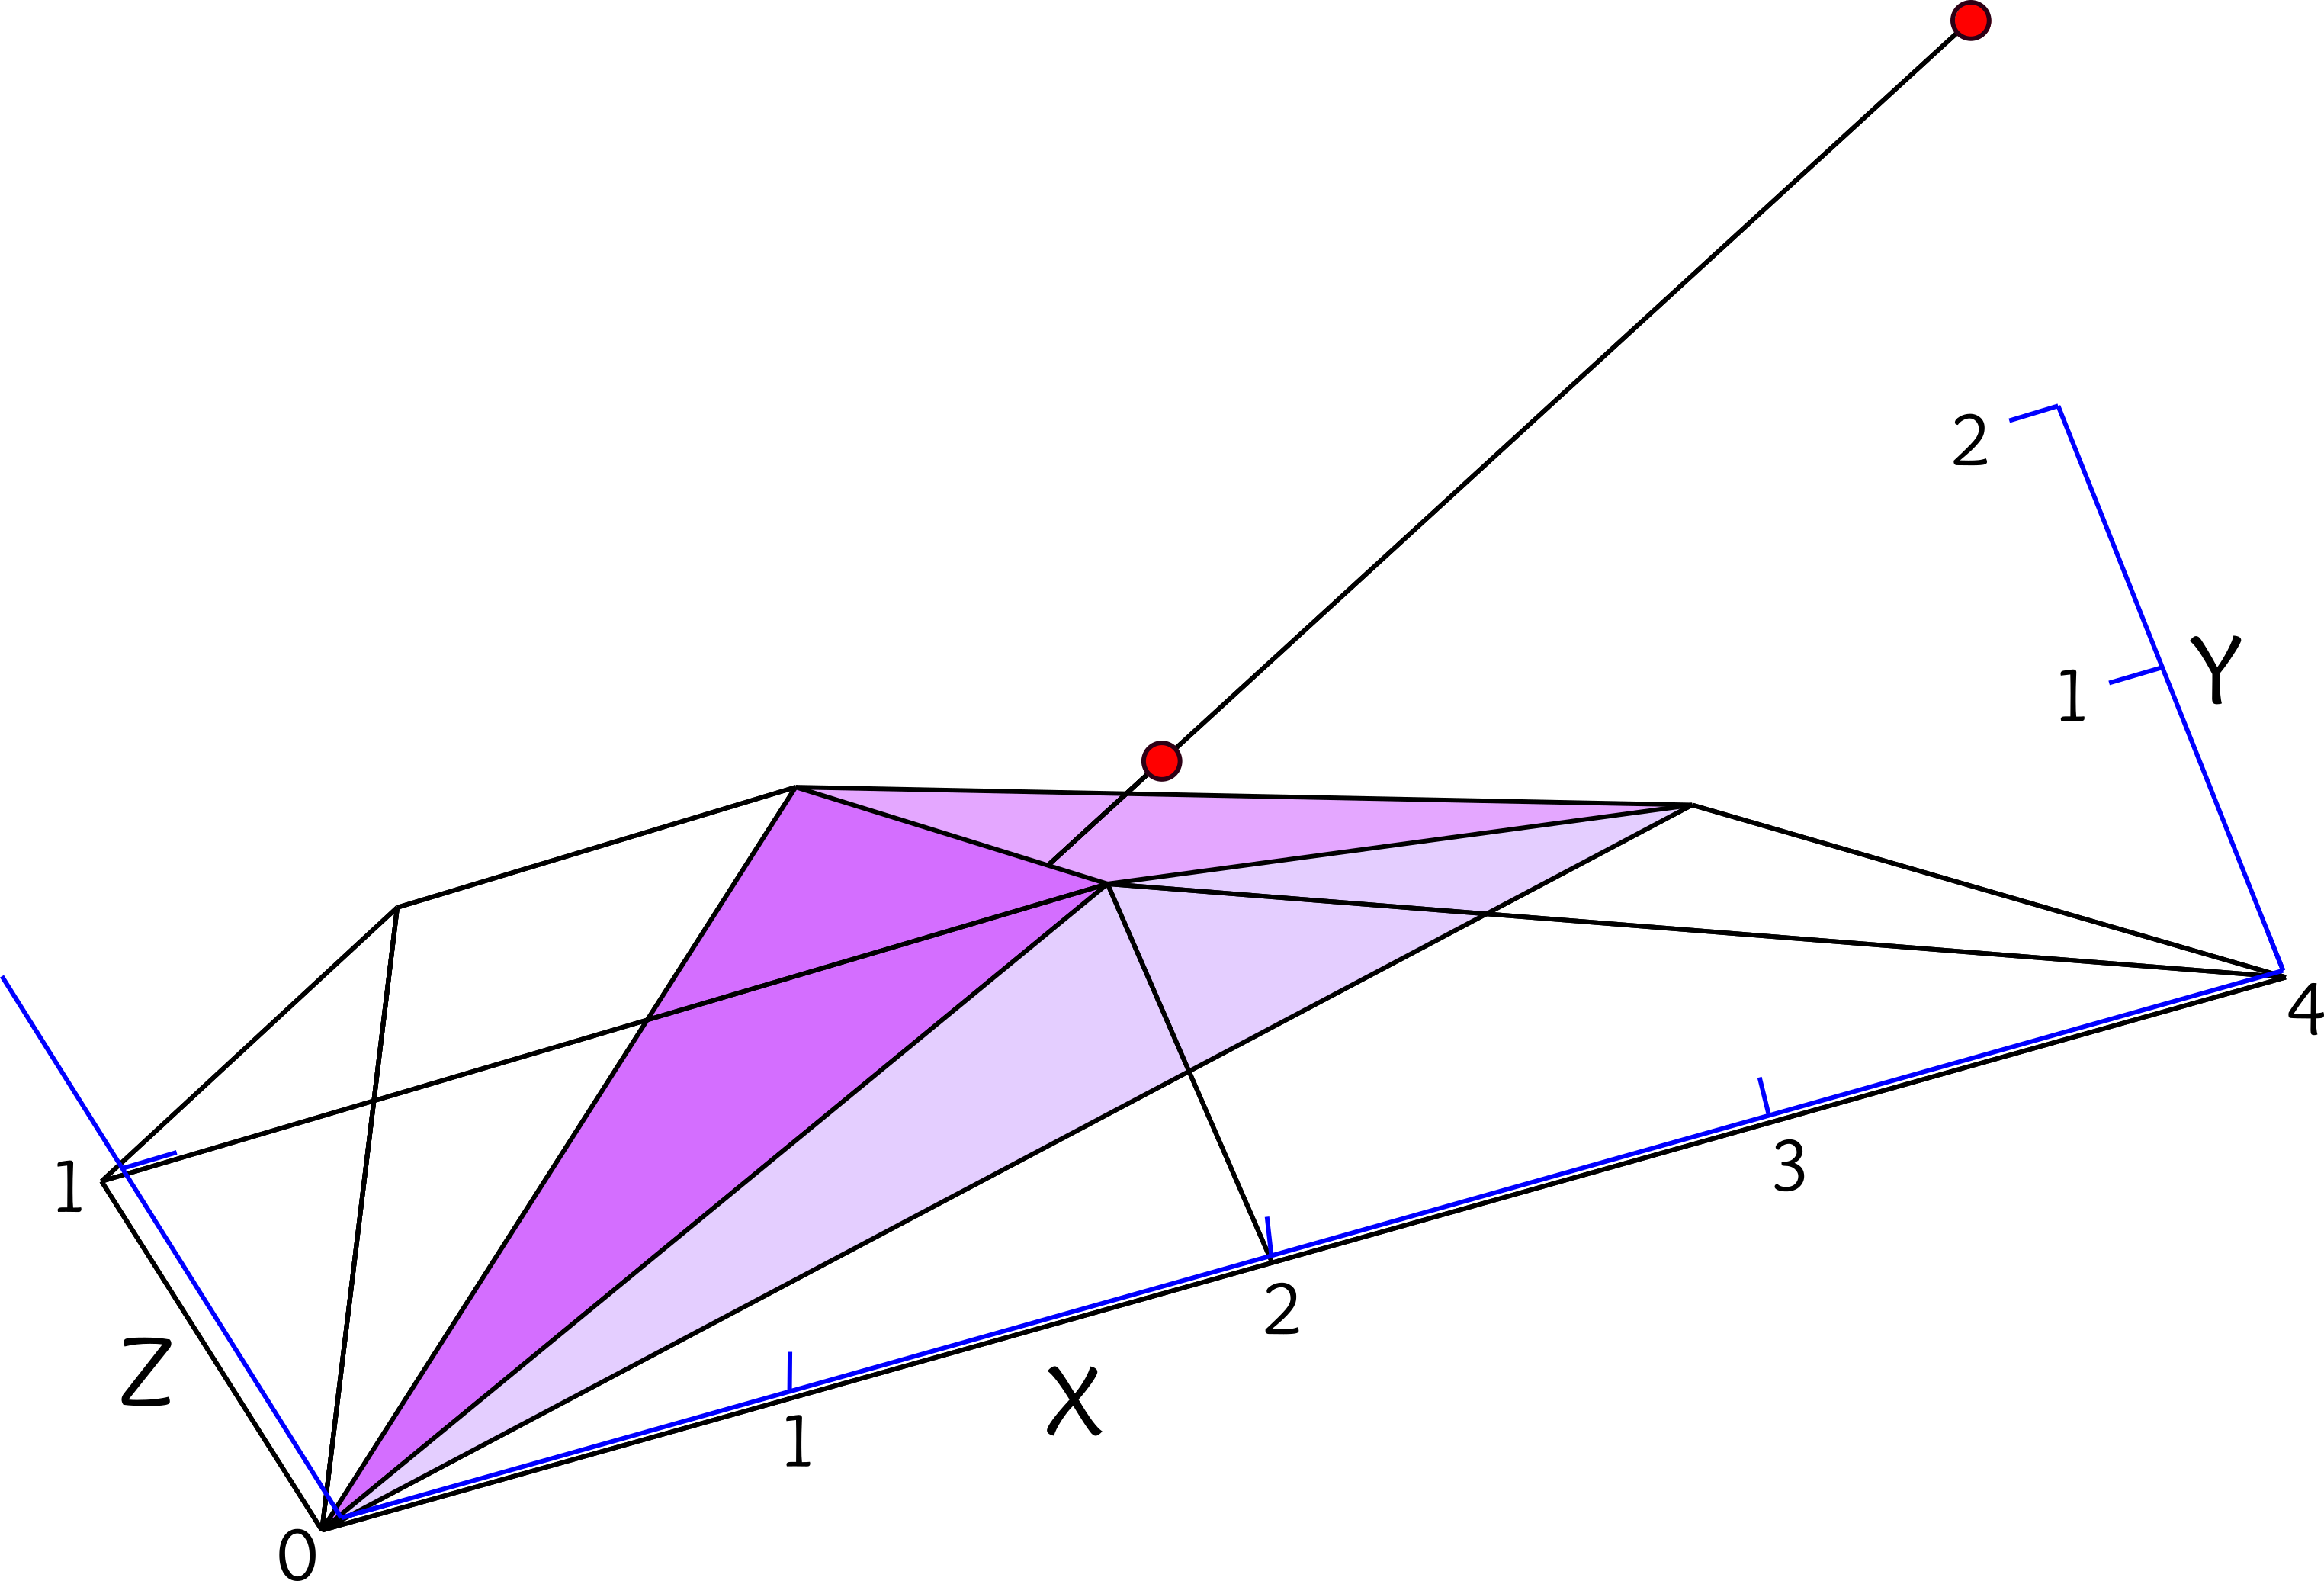
\includegraphics[scale=0.45]{figure/feasibility-good1.png}}
    \end{center}
\end{frame}


\begin{frame}{Modified Feasibility Certificate}
    
    \textbf{\b{Corresponding Polytope:}} For a bottleneck instance $I = (n,s,b,C,m)$ and the polytope $\mathsf{P} = \{x \in \mathbb{R}^n \mid s^{\text{T}} x \leq C, 0 \leq x \leq b_i, \ \forall i \in [n]\}$, then $\mathsf{P}^* = \text{conv}(\mathsf{P} \cap \mathbb{Z}^n)$ is the corresponding polytope. \\~\\
    
    \begin{alertblock}{Modified Theorem}
        For an instance $I = (n,s,b,C,m)$ and its corresponding polytope $\mathsf{P}^*$, $I$ is infeasible \emph{if} $\overline{b} = \frac{b}{m} \notin \mathsf{P}^*$. Otherwise, $I$ might be \a{feasible}.
    \end{alertblock}
    
\end{frame}


\begin{frame}{Some Definitions}
    \onslide<1->{Suppose $X \subseteq \mathbb{R}^n$ is a set of points. Then,
    
    \begin{equation*}
        \mathsf{C}(X) = \text{cone}(X) = \big\{\sum_{x \in X} \lambda_x \cdot x \mid \lambda_x \in \mathbb{R}_{\geq 0}, \forall x \in X \big\} \\
    \end{equation*}}
    
    \only<2>{\begin{center}
        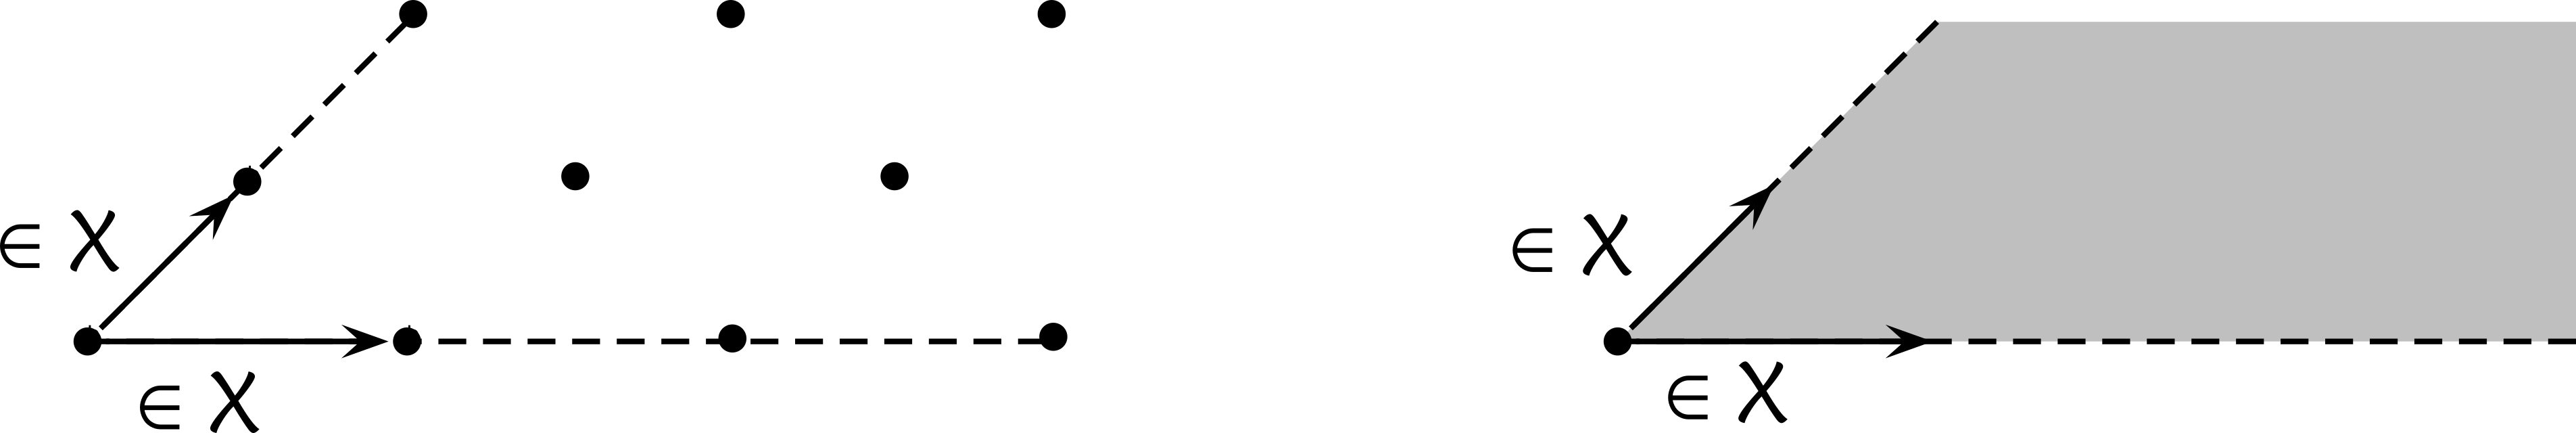
\includegraphics[scale=0.6]{figure/cone-int-cone.png}
    \end{center}}
    
    \onslide<3->{\textbf{\a{Assumption:}} All cones are pointed!}
    
    \onslide<3->{\textbf{\b{Caratheodary Thm:}} If $b \in cone(X)$, then there is a conic combination $\lambda \in \mathbb{R}^{X}_{\geq 0}$ with only $|\text{supp}(\lambda)| \leq n$ many non-zero entries and $b = \sum_{x \in X} \lambda_x \cdot x$.}
\end{frame}


\begin{frame}{Concentric Cones}
    
    % \only<1,2>{\textbf{\b{Closed Convex Cone:}} Given corresponding polytope $\mathsf{P}^*$ and facet $\mathsf{F} = \text{conv}\{f_1, \ldots, f_n \mid f_i \in \partial\mathsf{P}^*, \forall i \in [n]\}$ be an arbitrary facet of $\mathsf{P}^*$. A smallest closed convex cone is defined by $\mathsf{C}(\mathsf{F}) = \text{conv}(\mathbf{0}, \mathsf{F}) \subseteq \mathsf{P}^*$.}
    
    \onslide<1->{\textbf{\b{Concentric Convex Cones:}} Given $l$ $n$-dimensional convex cones $\mathsf{C}_i$, we call them concentric if they satisfy that $\mathsf{C}_1 \subset \mathsf{C}_2 \subset \ldots \subset \mathsf{C}_l$, where $C_i = \text{conv}(\mathbf{0}, \mathsf{F}_i), \ \forall i \in [l]$ and $ \mathsf{F}_i = \text{conv}(i \cdot f_i, \ldots, i \cdot f_n)$. In particular, all $\mathsf{C}_i$ are closed.}
    
    \onslide<2->{\begin{center}
        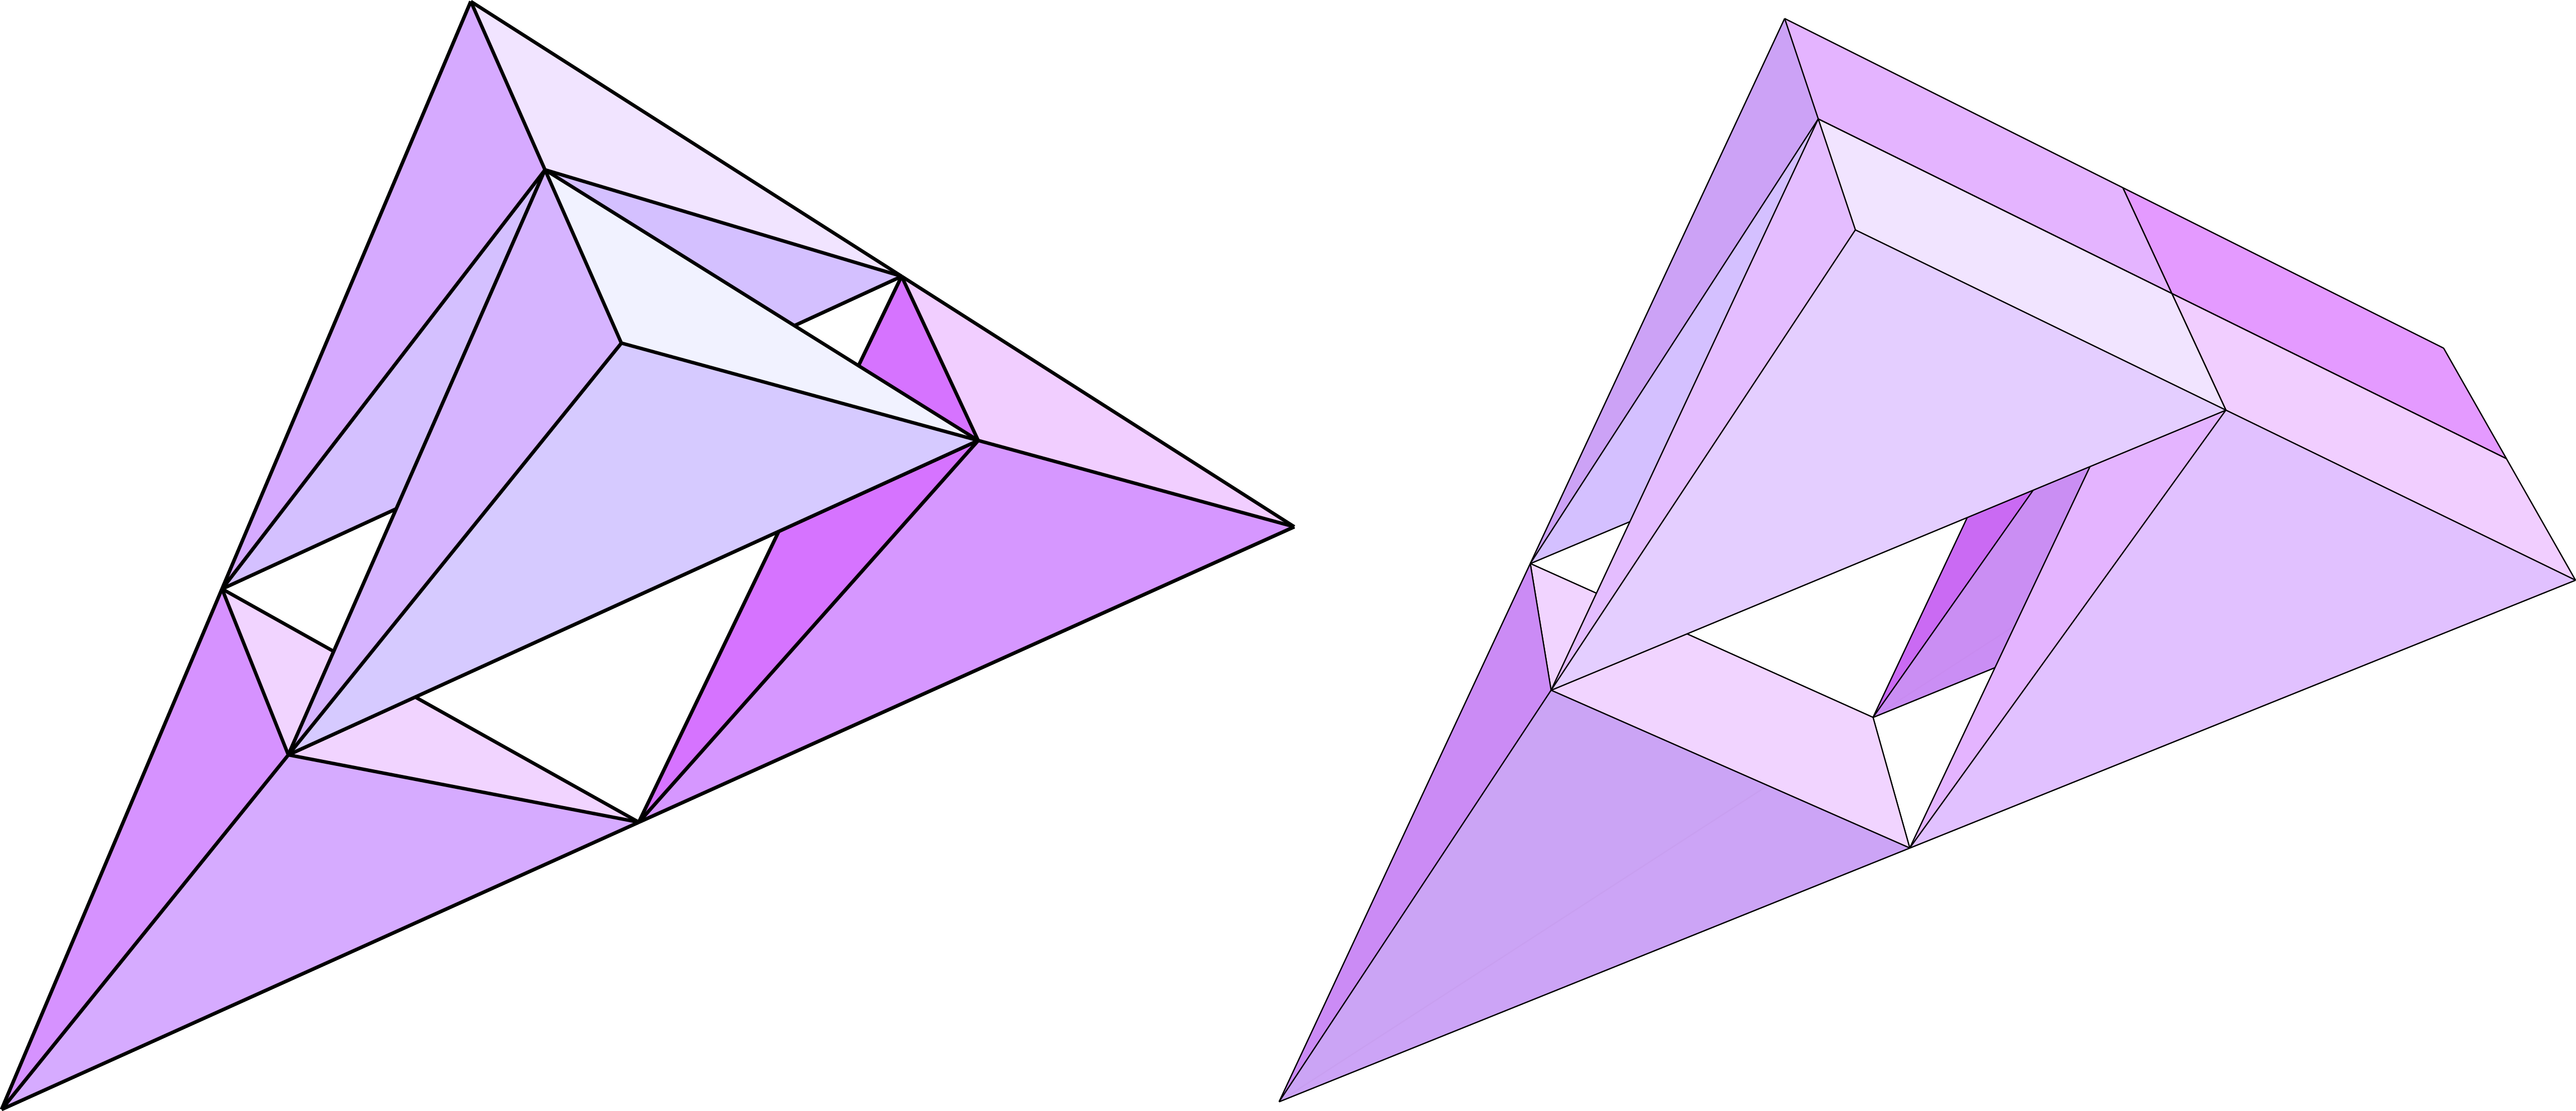
\includegraphics[scale=0.5]{figure/concentric-cone-two.png}
    \end{center}}
\end{frame}


\begin{frame}{Structural Theorem: Construction of Solution}

    \onslide<1->{\begin{block}{Theorem}
        \onslide<1->{Given $I = (n,s,b,C,m)$ and $\frac{b}{m} \in \mathsf{P}^*$.} \onslide<2->{Let $\mathsf{F}_1 = \{f_1, \ldots, f_l\} \subseteq \mathsf{P}^*$ induced by the intersection of straight line between $\mathbf{0}$ and $b$.} \onslide<3->{Then $\exists$ concentric cones $\mathsf{C}_1 \subset \mathsf{C}_2 \subset \ldots \subset \mathsf{C}_m$} \onslide<4->{with $b \in \mathsf{C}_m$ s.t. $b$ can be represented by $O(n)$ integral vectors chosen from the vertices of $\mathsf{F}_1$ or dominated by these, and an integral residue $r \in \mathsf{P}^*$.} 
    \end{block}}
    
    \only<2,4>{\begin{center}
        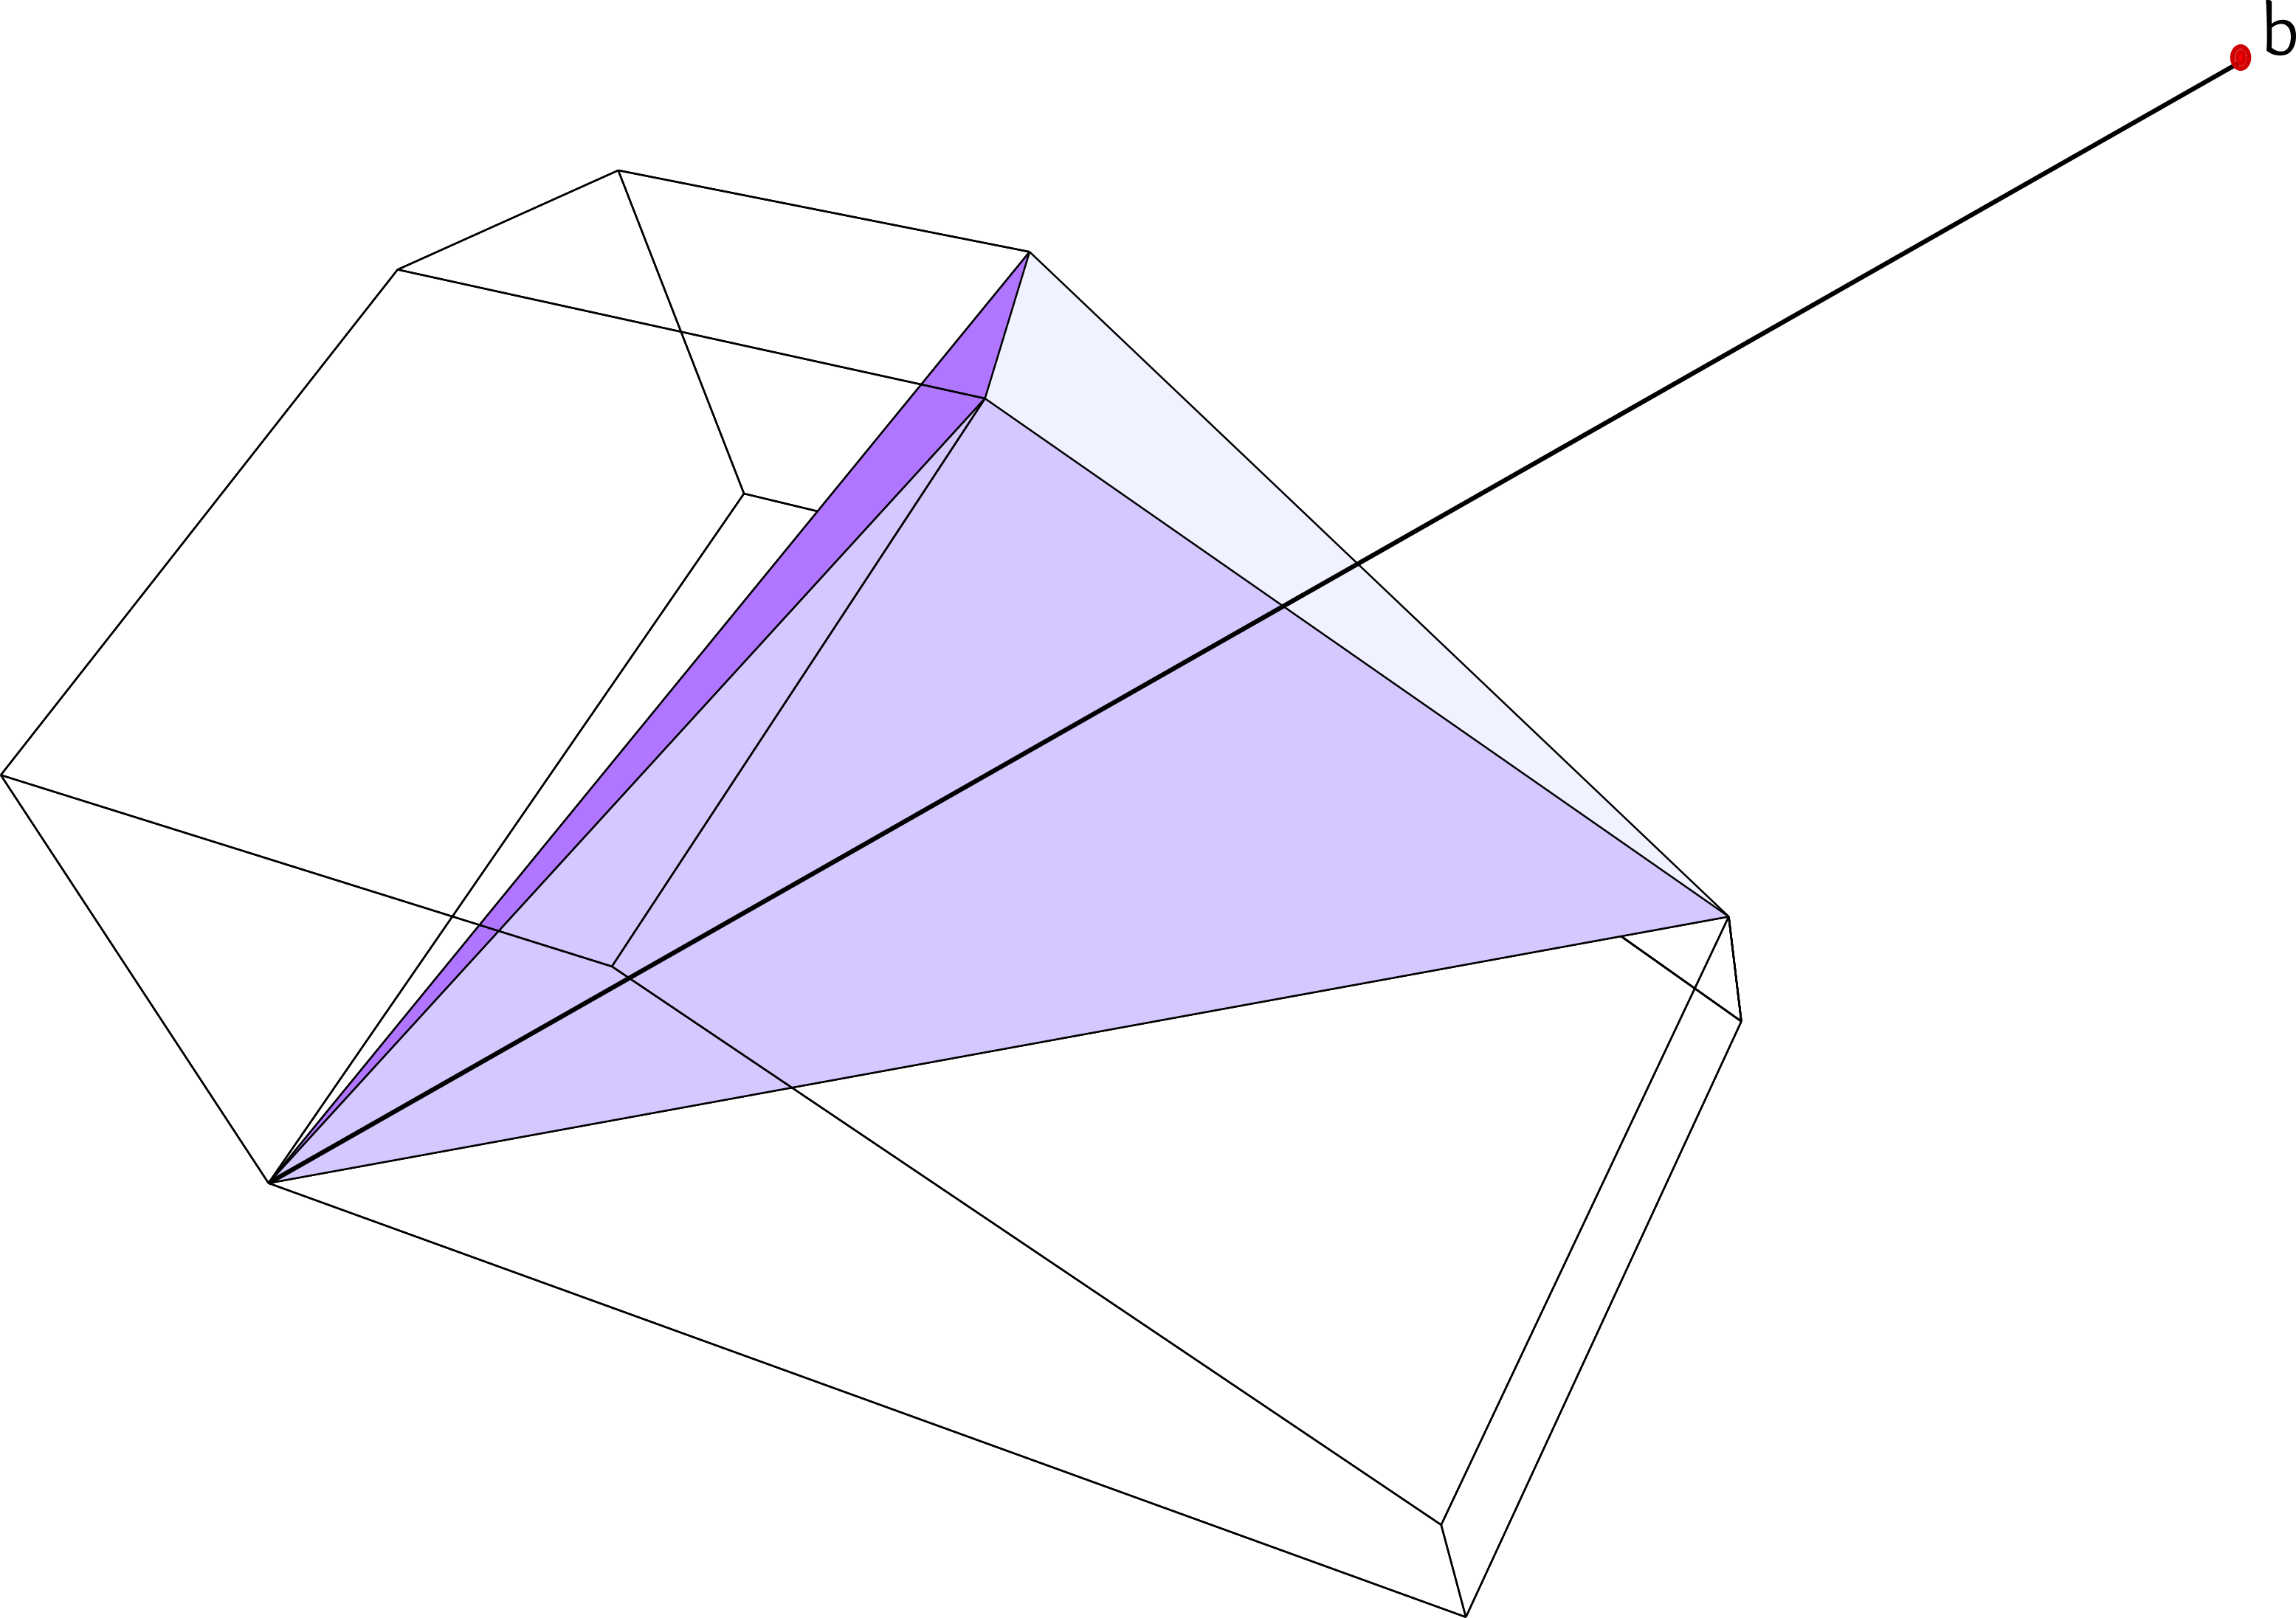
\includegraphics[scale=0.45]{figure/thm-explain.png}
    \end{center}}
    
    \only<3>{\begin{center}
        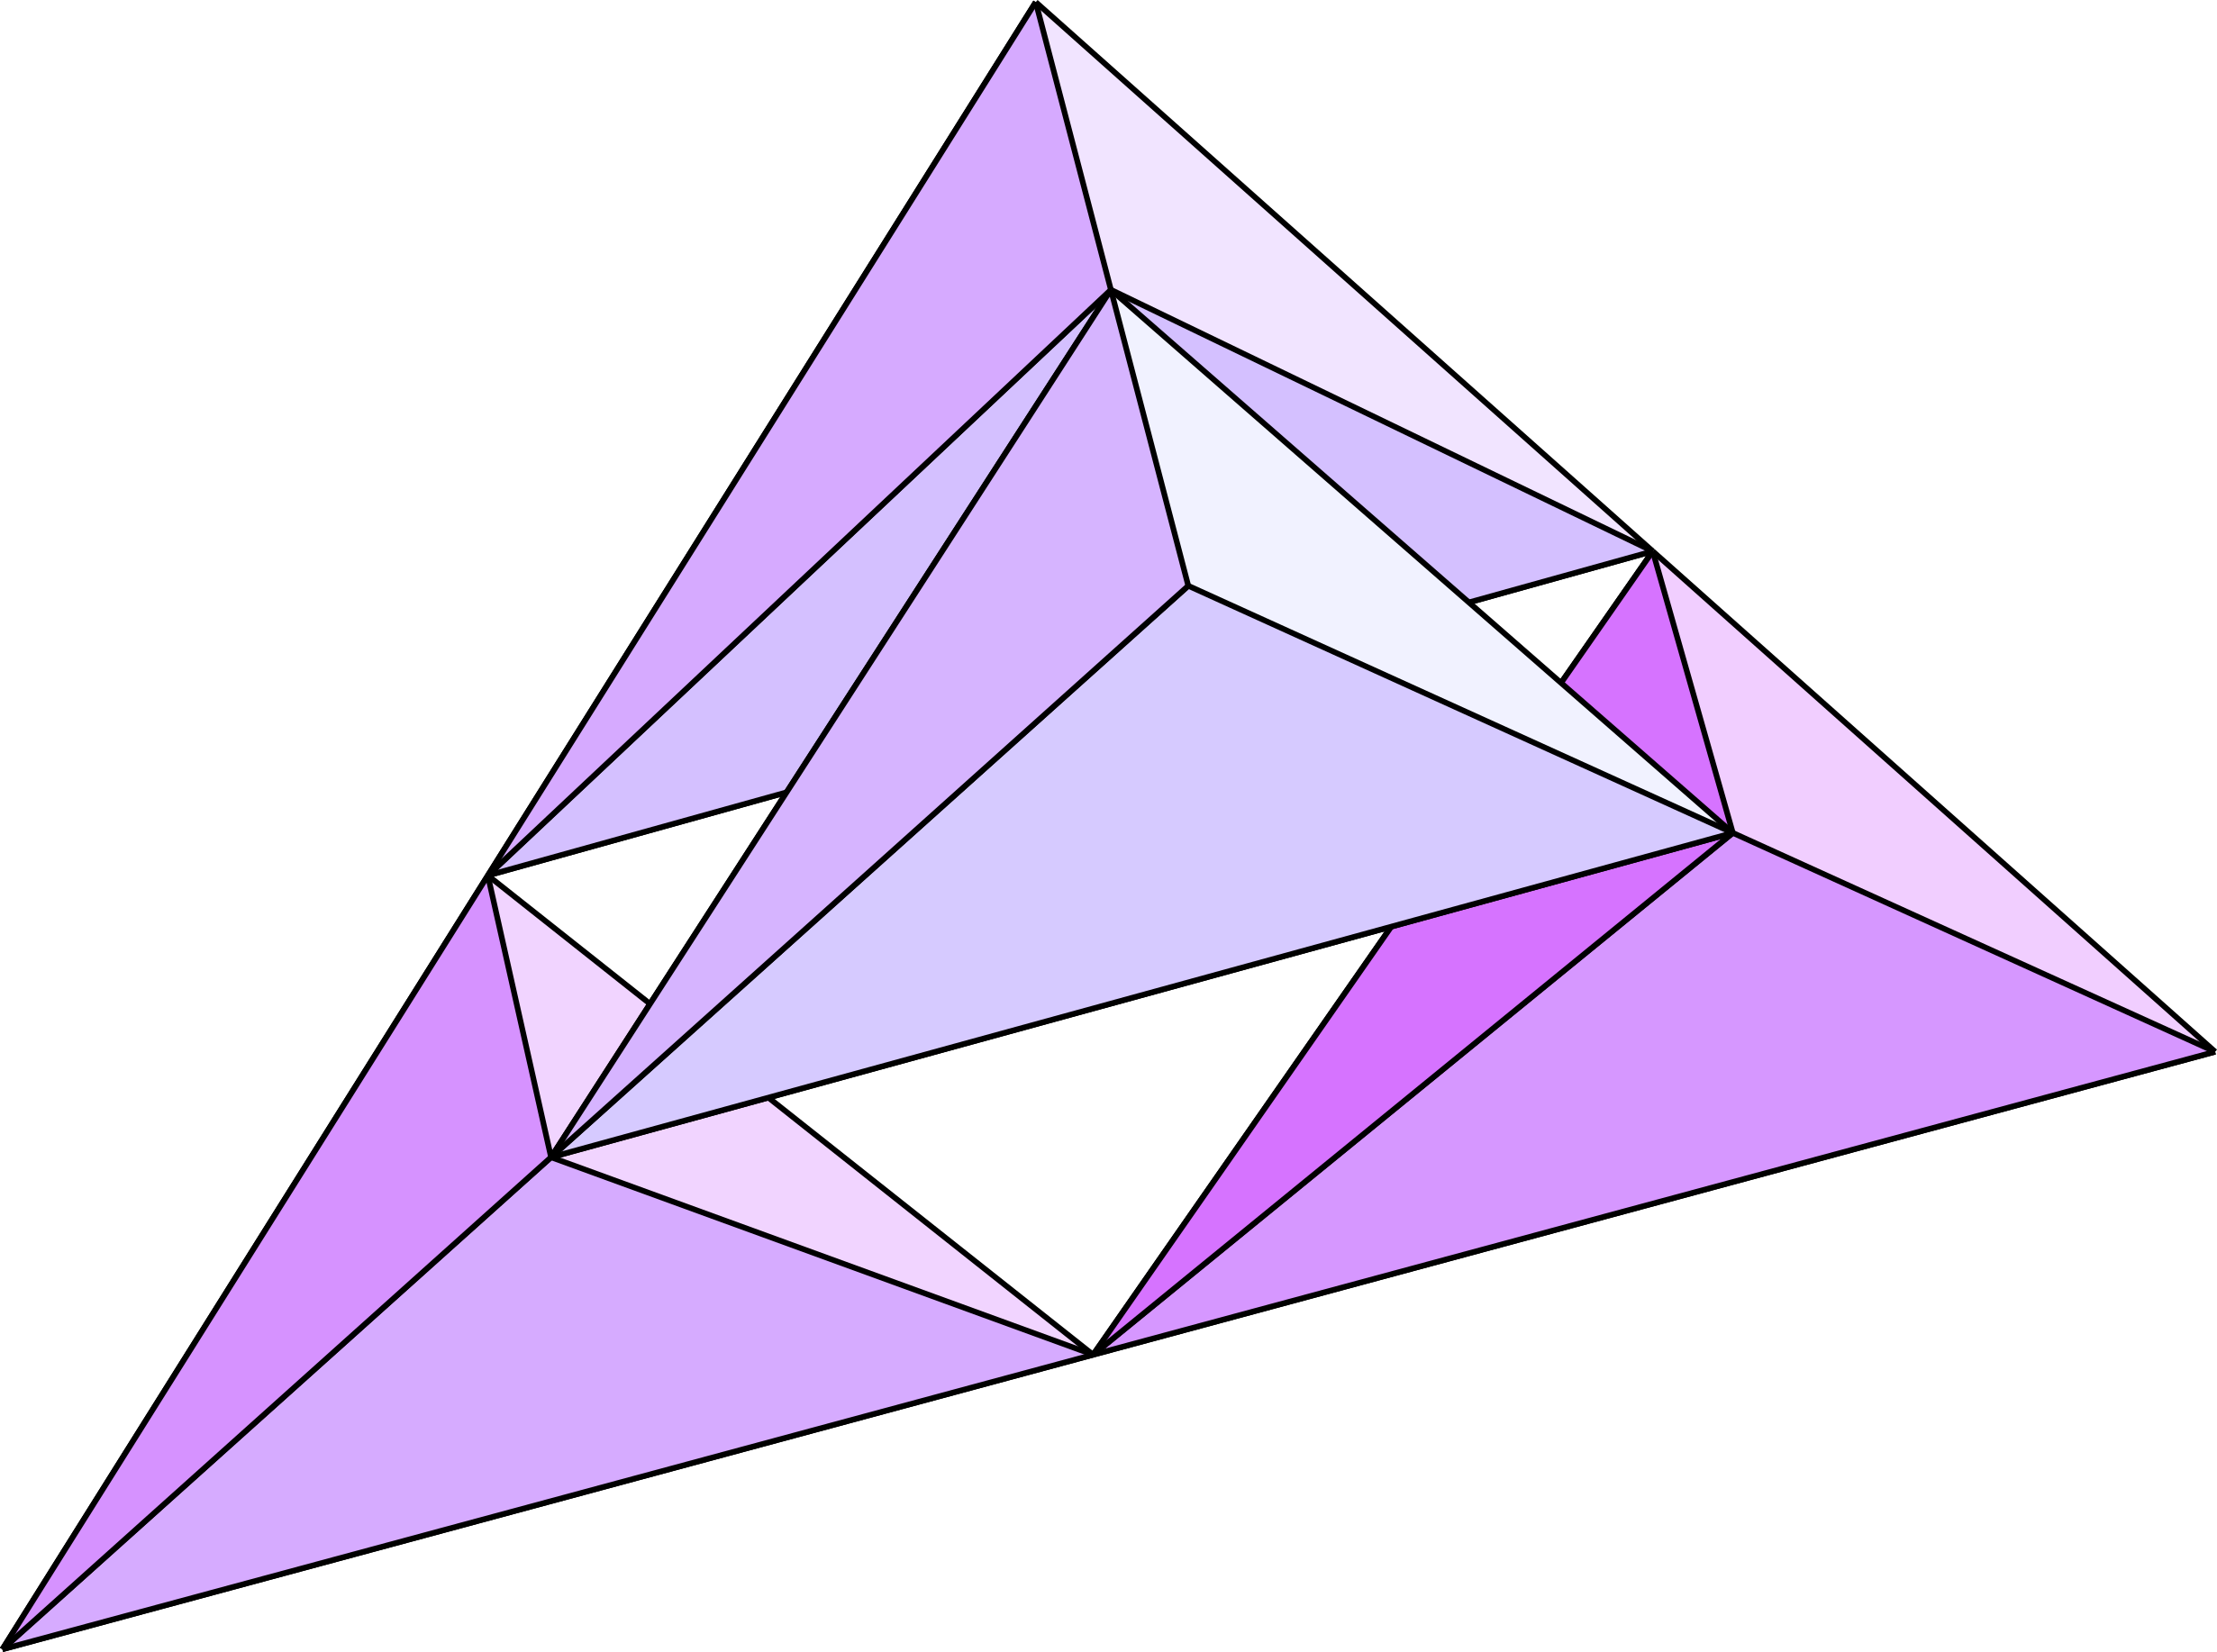
\includegraphics[scale=0.4]{figure/concentric-cone-polytope.png}
    \end{center}}

    
\end{frame}

\begin{frame}{Construction of Solution: Proof Case 1,2,3}
    % \textbf{\b{Assumptions:}} W.l.o.g. $\mathsf{C}_1$ is simplicial and $\mathsf{C}_1 = \text{conv}(\mathbf{0}, f_1, \ldots, f_n)$. Also $b \in \mathsf{C}_m \setminus \mathsf{C}_{m-1} = \text{conv}(\mathsf{F}_m, \mathsf{F}_{m-1})$.  
    
    % \begin{itemize}
    %     \item Proof by induction over $m$.
        
    %     \item \b{Base case:} $m = 1$ is correct as $b \in \mathsf{C}_1$ is represented by itself.
        
    %     \item By $\text{def}^{\text{n}}$ of concentric cones, every point in $\mathsf{F}_{m+1}$ can be translated back to $\mathsf{F}_2$ using $m$ integral points from facet $\mathsf{F}_1$ defining vertices.
        
    %     \item As $\mathsf{C}_2 = \text{conv}(\mathbf{0}, \mathsf{F}_2)$ is built uniformly by extending $\mathsf{C}_1$
        

    % \end{itemize}
    %         \a{$\implies$ it suffices to show that any integral point from $\mathsf{C}_2 \setminus \mathsf{C}_1$ can be translated to an integral point in $\mathsf{P}^*$.}
    
        \begin{center}
        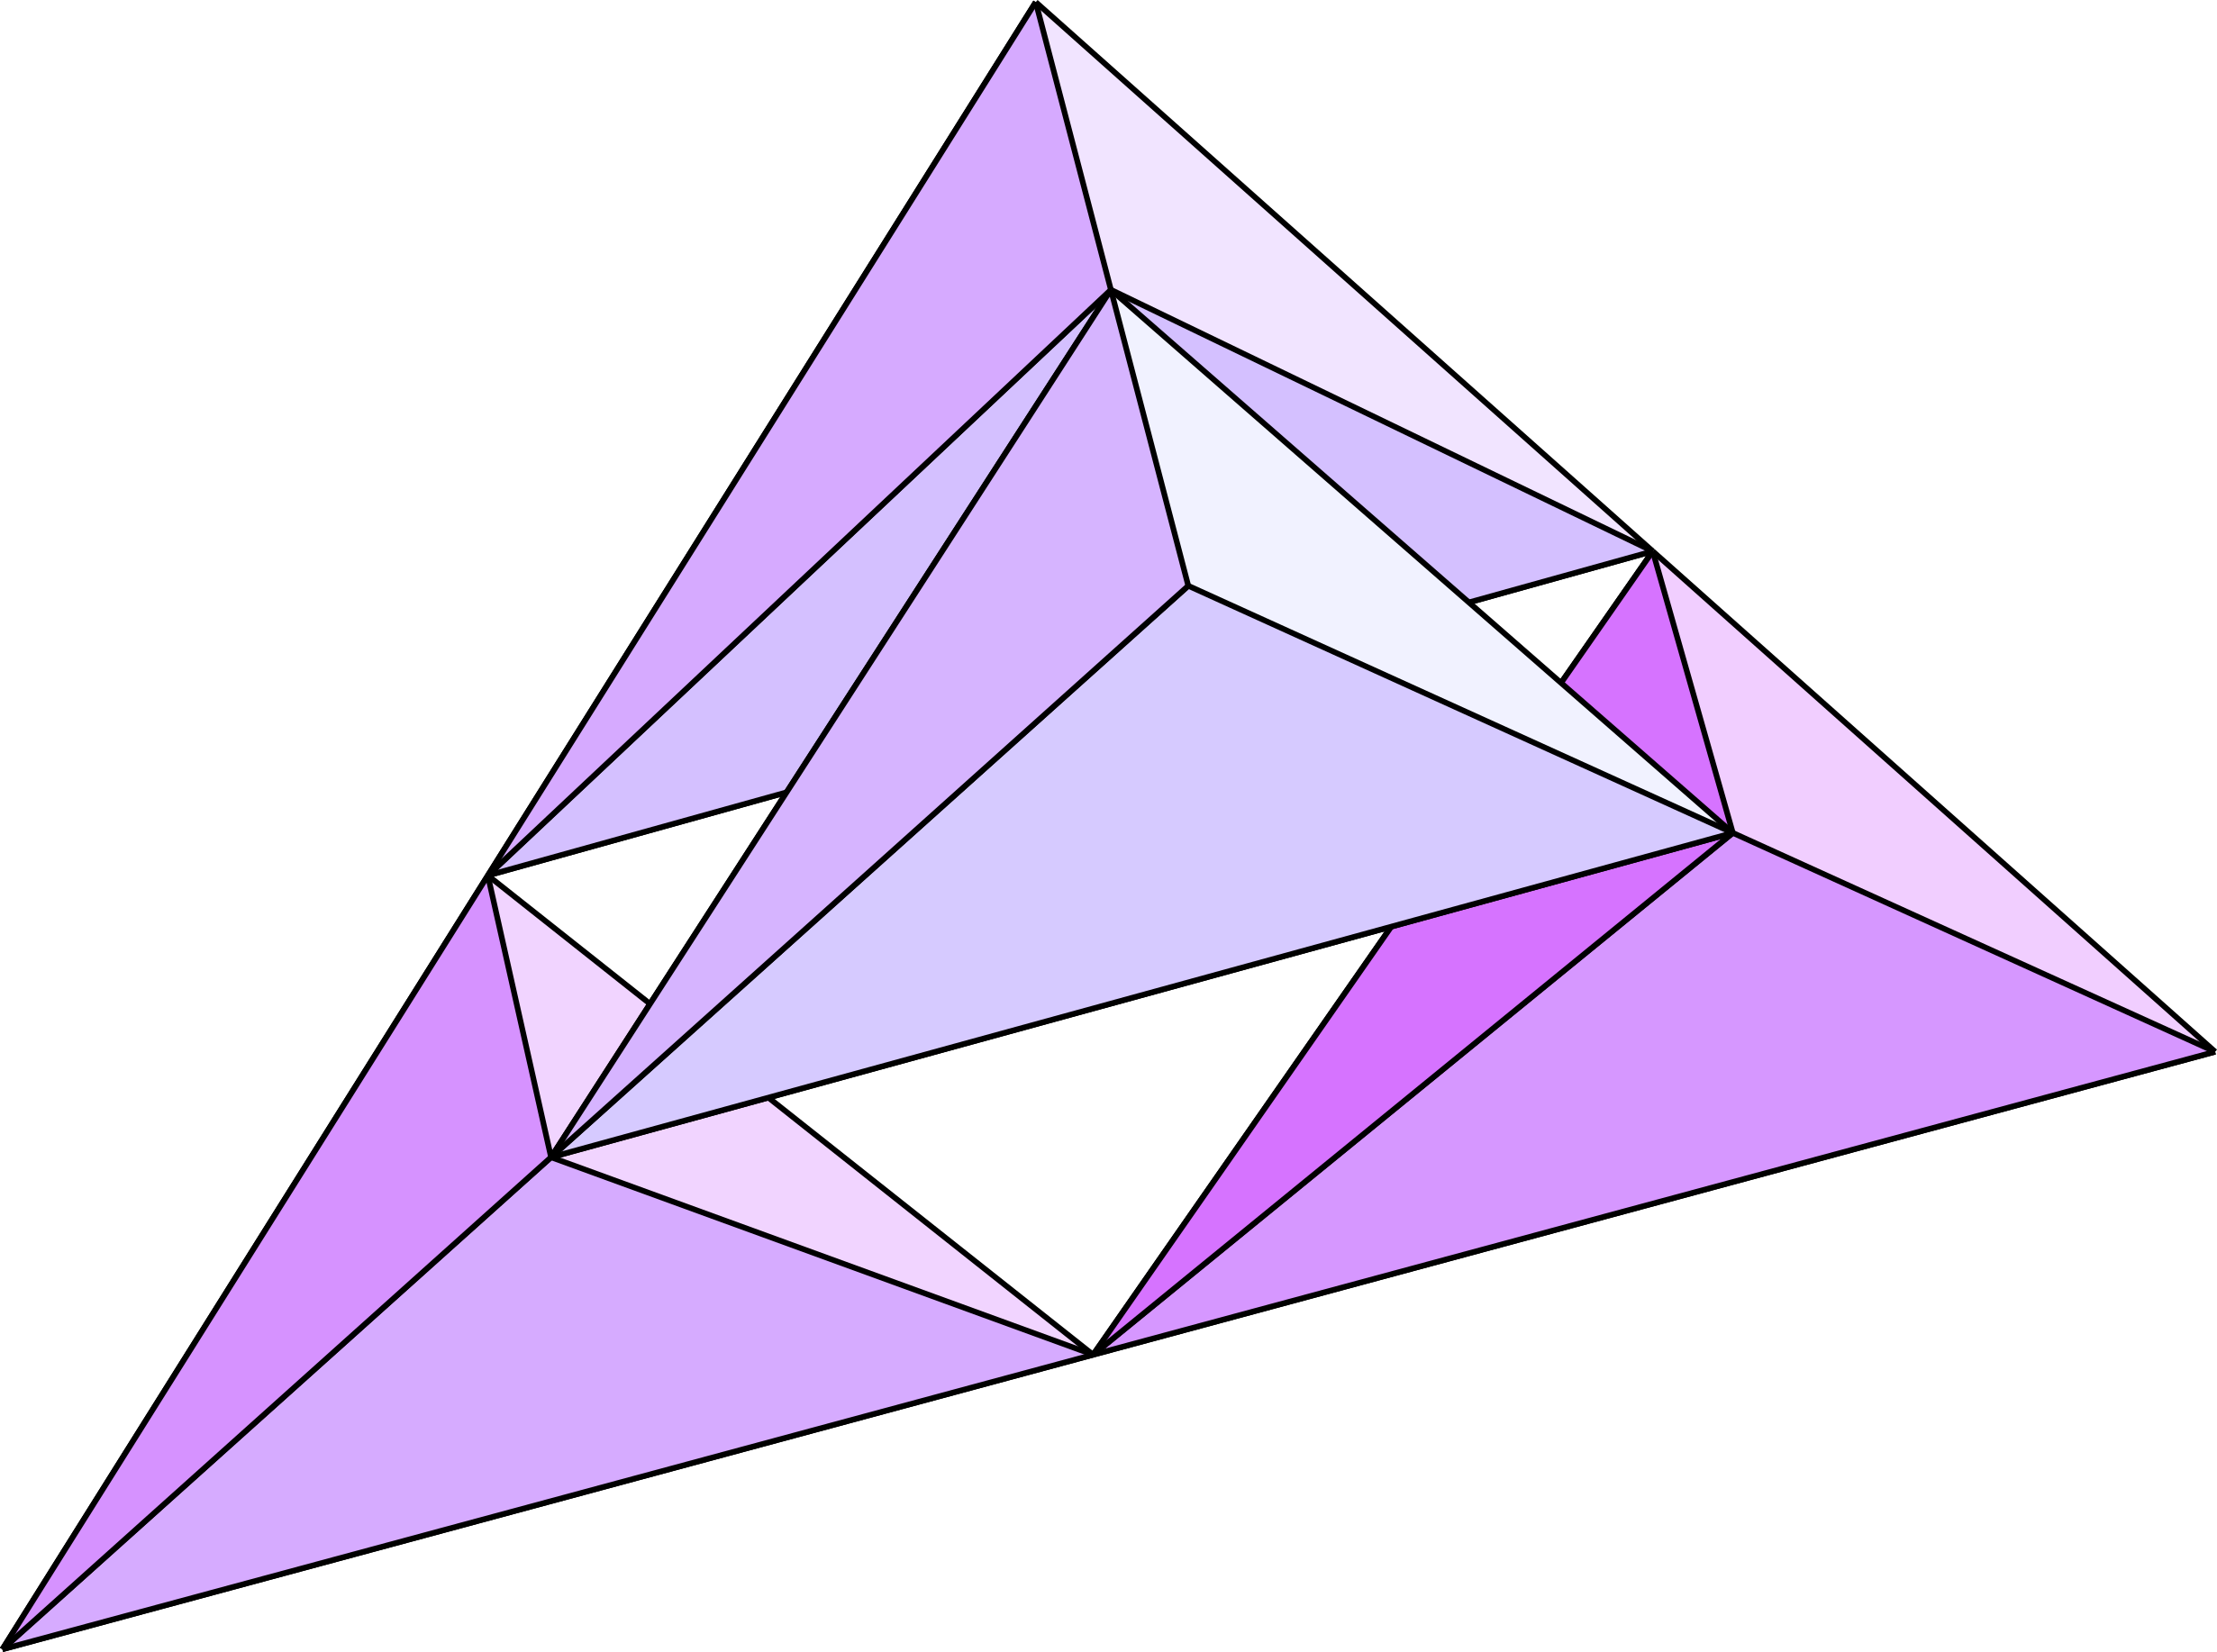
\includegraphics[scale=1]{figure/concentric-cone-polytope.png}
    \end{center}
\end{frame}


% \begin{frame}{Construction of Solution: Theorem Proof (2)}

% Consider $r \in (\mathsf{C}_2 \setminus \mathsf{C}_1) \cap \mathbb{Z}^n$. Clearly, $r \in \text{conv}(f_1, \ldots, f_n, 2 f_1, \ldots, 2 f_n)$.

%     \begin{itemize}
%         \item \textbf{\b{Case 1:}} \textbf{$r$ resides in one of the $n$ copies of $\mathsf{C}_1$ originating at $f_i$.}
%         \begin{itemize}
%             \item Can be easily translated to a point in $\mathsf{F}_1 \subset \mathsf{P}^*$ by translation vector $x = r - f_j$, where $f_j \in \mathsf{F}_1 \cap \mathbb{Z}^n \a{\implies x \in \mathsf{C}_1 \subseteq \mathsf{P}^*}$. 
%         \end{itemize}
        
%         \item \textbf{\b{Case 2:}} \textbf{$r$ is dominated by an integral point from one of the $n$ copies of $\mathsf{C}_1$.}
        
%             \begin{itemize}
%                 \item Analogous to \textbf{\b{Case 1}}. 
%             \end{itemize}
%     \end{itemize} 
% \end{frame}


% \begin{frame}{Construction of Solution: Theorem Proof (3)}
%     \begin{itemize}
    
%         \item \textbf{\b{Case 3:}} \textbf{Neither \b{Case 1} nor \b{Case 2}. (i.e. $r$ is maximal)}
        
%         \begin{itemize}
%             \item $r \in \text{conv}(2f_1, \ldots, 2f_l) = \sum_{i=1}^{l} \lambda_i \cdot 2f_i$, where $\sum_{i=1}^{l} \lambda_i = 1$, $r \in \mathbb{Z}^n$.
            
%             \begin{equation*}
%                 \begin{aligned}
%                     s^\text{T} r = \sum_{i=1}^{l} s \cdot \lambda_i \cdot 2f_i = 2 \sum_{i=1}^{l} s \cdot \lambda_i \cdot f_i \leq 2C
%                 \end{aligned}
%             \end{equation*}
%             $\centernot\implies$ $\a{\text{r is not necessarily representable by 2 integral pts from} \ \mathsf{C}_1.}$
%         \end{itemize}
        
%         \item \textbf{\b{Lemma:}} $\exists$ at least one integral vertex $z = f_j + f_k \in \mathsf{F}_2$ with $f_j, f_k \in \mathsf{F}_1$ and a point $x = z - r$ such that $x^+$\footnote{$x^+$ is the resulting vector from projecting all negative components of $x$ to zero.}
%         % \footnote{$x^+ = (x_1^+, \ldots, x_n^+)$, where $\textstyle x_i =           \begin{cases}
%         %     x_i, & \text{if $x_i > 0$}\\
%         %     0, & \text{otherwise.}
%         %     \end{cases}$} 
%         is a feasible pattern w.r.t. bin capacity $C$ and $x^+ \in \mathsf{P}^*$. \QEDA 
%     \end{itemize}
    
% \end{frame}

% \begin{frame}{Summary of Theorem Proof}
%     \begin{itemize}
%         \item We study the \a{\emph{holes}} on $\mathsf{F}_2$ defining $\mathsf{C}_2$.
        
%         \item A linear translation $-f, f \in \{f_1, \ldots, f_n\}$ of a vector contained in such \emph{holes} to $\mathsf{P}^*$ does not necessarily belong to $\mathsf{P}^*$.
        
%         \item This alludes that integral points within $\mathsf{C}_2$ cannot be represented by two points from $\mathsf{F}_1$ defining vertices or dominated by them.
        
%         \item Hence, we show that one extra point from $\mathsf{P}^*$ suffices to cover the points located in the \emph{holes}.
        
%         \item This is because the axial extensions of $\mathsf{P}^*$ are defined by vertices of $\mathsf{F}_1$. 
        
%         \item Hence the resulting vectors $x^+$ with negative components mapped to zero are in $\mathsf{P}^*$.
%     \end{itemize}
% \end{frame}

\begin{frame}{Computation of Relevant Patterns: Conditions}
    \b{Want to find explicit representation of $\mathsf{F} \subset \mathsf{P}^*$ satisfying following conditions:}
    
    \begin{itemize}
        \item $\frac{b}{m} \in \text{conv}(0, f_1, \ldots, f_n)$. 

        \item $\frac{s^\text{T} b}{m} \leq s^\text{T} f_i \leq \widetilde{C}$, for all $i \in [n]$, where $\widetilde{C}$ is defined according to the upper bound $UB$.
        
        \item all $f_i$ are linearly independent.
    \end{itemize}
    
    \textbf{\b{Hindrance:}} 
        \begin{itemize}
            \item No explicit representation of the corresponding polytope $\mathsf{P}^*$.
        \end{itemize}
\end{frame}


\begin{frame}{Explicit Representation of $\mathsf{P}^*$}
    \begin{alertblock}{Integral points in $\mathsf{P}^*$~\cite{cook1992integer, hartmann1988cutting}}
    Let $V^*$ be the vertices of $\mathsf{P}^*$. Then $|V^*| \leq m^n \cdot (O(\log( \Delta)))^n$ and can be computed in $|V^*| \cdot n^{O(n)} \cdot (m \log (\Delta))^{O(1)}$.
    \end{alertblock}
    
    \begin{itemize}
        \item As $n$ is fixed, the explicit representation of $\mathsf{P}^*$ can be computed in polynomial time.
        
        \item Let $V^* = \{p_1, \ldots, p_k\}$ be the vertex set that define $\mathsf{P}^*.$
    \end{itemize}
    
\end{frame}

\begin{frame}{Computation of Relevant Patterns: Primal Dual Algorithm}

    \begin{itemize}
        \item $\frac{b}{m} \in \text{conv}(0, f_1, \ldots, f_n)$. 

        \item $\frac{s^\text{T} b}{m} \leq s^\text{T} f_i \leq \widetilde{C}$, for all $i \in [n]$, where $\widetilde{C}$ is defined according to the upper bound $UB$.
        
        \item all $f_i$ are linearly independent.
    \end{itemize}
    

        \begin{itemize}
            \item Can compute the vertices $\{f_1, \ldots, f_n\}$ using Primal-Dual method.
            
            \item To check the feasibility of the solution to the dual LP, we solve the separation problem which is knapsack problem in fixed dimension.
        \end{itemize}
\end{frame}

% \begin{frame}{Computation of Relevant Patterns: Primal-Dual Algorithm}

% \onslide<1->{\begin{tabular}{cl}  
%          \begin{tabular}{c}
%           \parbox{0.2\linewidth}{%  change the parbox width as appropiate
%             \textbf{\b{Primal:}}
%     }

%           \end{tabular}
%           & \begin{tabular}{l}
%           \centering
%                 \begin{equation*}
%                 \begin{medsize}
%                     \begin{aligned}
%                         & {\text{max}}
%                         & & y \\
%                         & \text{s.t.} & & \sum_{i=1}^{k} \alpha_i \: p_{i, j} = y \: b_j &&&& \forall j \in [n], \ \sum_{i=1}^{k} \alpha_i = 1 \\
%                         & & & \alpha_i \geq 0 &&&& \forall i \in [n] \\
%                         & & & y \geq 0 
%                     \end{aligned}
%                 \end{medsize}
%                 \end{equation*}
%          \end{tabular}  \\
% \end{tabular}}

% \onslide<2->{\begin{tabular}{cl}  
%          \begin{tabular}{c}
%           \parbox{0.2\linewidth}{%  change the parbox width as appropiate
%           \textbf{\b{Dual:}}
%     }

%           \end{tabular}
%           & \begin{tabular}{l}
%           \centering
%                  \begin{equation*}
%                  \begin{medsize}
%                     \begin{aligned}
%                         & {\text{min}}
%                         & & z \\
%                         & \text{s.t.} & & \sum_{j=1}^{n} \lambda_j \: p_{i, j} + z \geq 0 &&&& \forall i \in [k] \\
%                         & & & \sum_{j=1}^{n} \lambda_j \: b_{j} \leq -1
%                     \end{aligned}
%                 \end{medsize}
%                 \end{equation*}
%          \end{tabular}  \\
% \end{tabular}}

% \onslide<3->{\begin{tabular}{cl}  
%          \begin{tabular}{c}
%           \parbox{0.2\linewidth}{%  change the parbox width as appropiate
%             \textbf{\b{Separation:}}
%     }

%           \end{tabular}
%           & \begin{tabular}{l}
%           \centering
%                 \begin{equation*}
%                  \begin{medsize}
%                     \begin{aligned}
%                         & {\text{max}}
%                         & & \lambda^\text{T} \: y \\
%                         & \text{s.t.} & & s^\text{T} \: y \leq C \\
%                         & & & y \in \mathbb{Z}^n_{\geq 0}
%                     \end{aligned} 
%                 \end{medsize}
%                 \end{equation*}
%          \end{tabular}  \\
% \end{tabular}}

% \end{frame}


\begin{frame}{From Patterns to Solution}
   \begin{itemize}
       \item \textbf{\b{Diophantine equation:}} $\sigma_1 f_1 + \ldots + \sigma_n f_n = b - r, \text{where} \ \sigma_i \in \mathbb{Z}_{\geq 0}, \ \forall i \in [n]$

        \only<2>{\item \textbf{\b{Problem:}} The residual $r$ is not known \b{\emph{a priori}}, and hence without $r$ the solution to the Diophantine equation is \a{not} necessary \b{integral}.}
        
        \onslide<3->{\begin{center}
            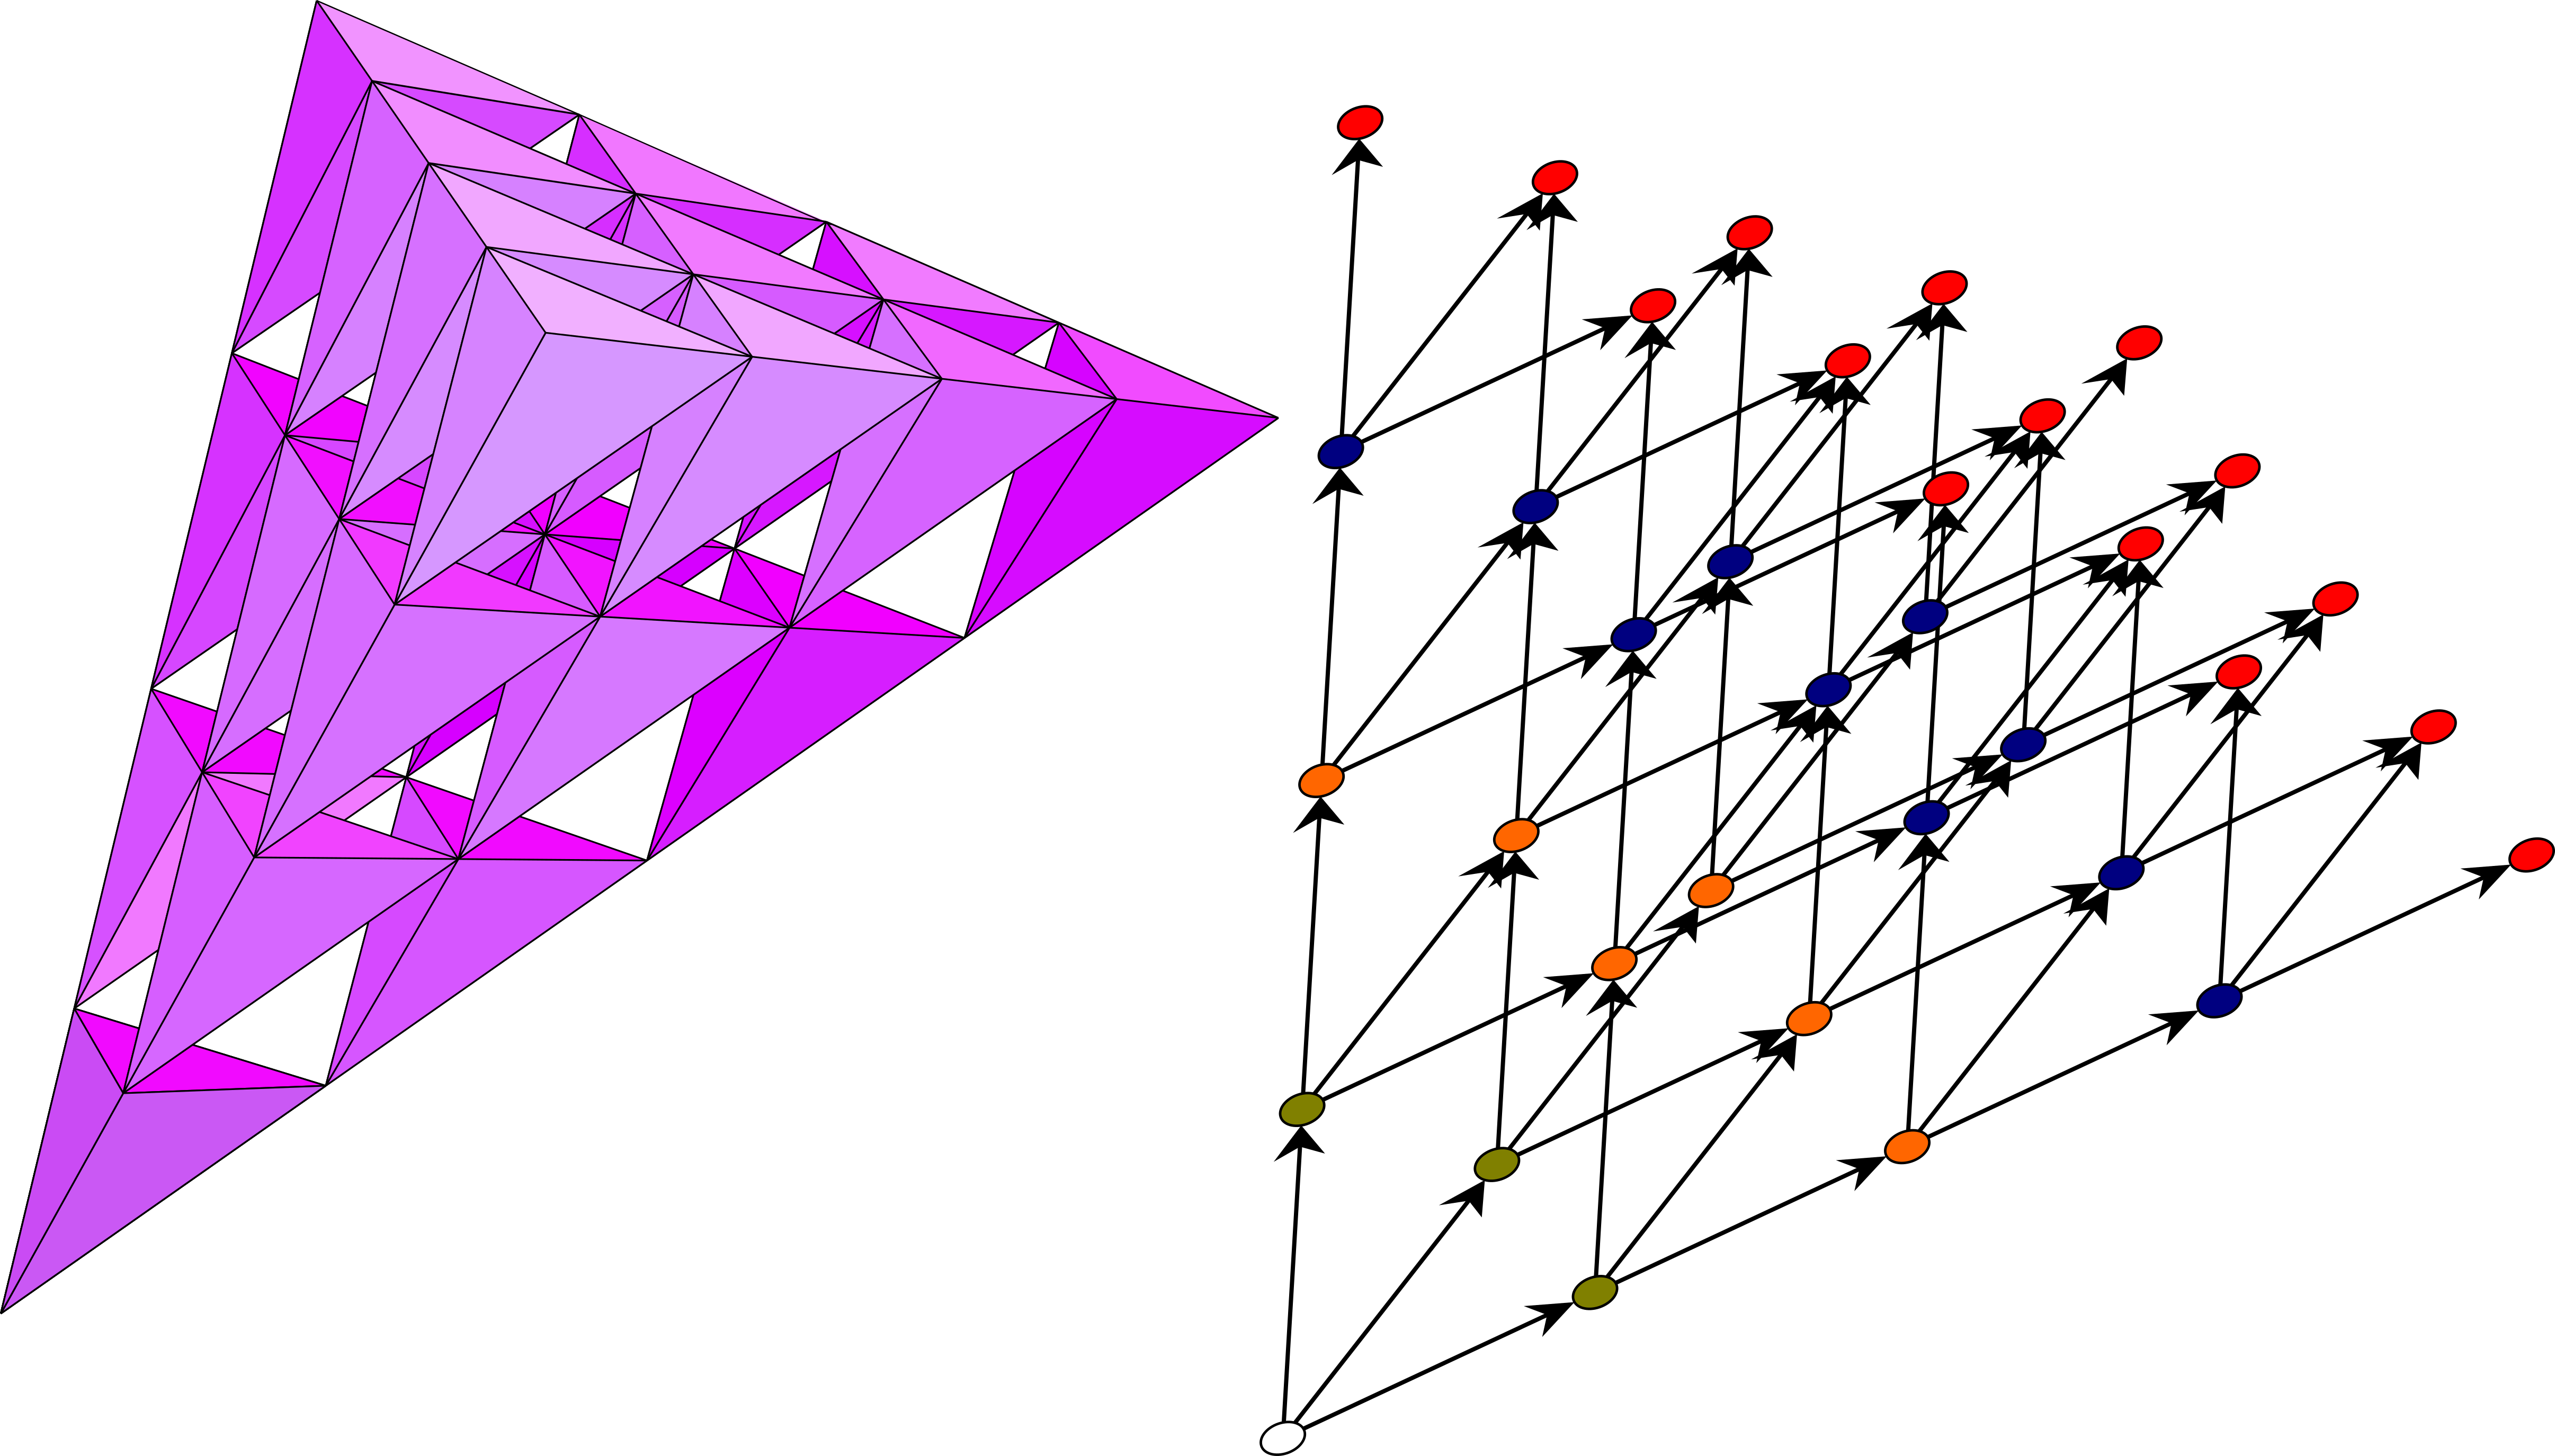
\includegraphics[scale=0.5]{figure/patterns-to-solution.png}
        \end{center}}
   \end{itemize}  
\end{frame}


\section{Thank You}


\begin{frame}[allowframebreaks]{References}
  \bibliography{global_divergences}
  \bibliographystyle{apalike}
\end{frame}

\end{document}

